%&preformat-disser
\RequirePackage[l2tabu,orthodox]{nag} % Раскомментировав, можно в логе получать рекомендации относительно правильного использования пакетов и предупреждения об устаревших и нерекомендуемых пакетах
% Формат А4, 14pt (ГОСТ Р 7.0.11-2011, 5.3.6)
\documentclass[a4paper,14pt,oneside,openany]{memoir}

%%%%%%%%%%%%%%%%%%%%%%%%%%%%%%%%%%%%%%%%%%%%%%%%%%%%%%%%%%%%%%%%%%%%%%%%%%%%%%%%
%%%% Файл упрощённых настроек шаблона, общих для диссертации и автореферата %%%%
%%%%%%%%%%%%%%%%%%%%%%%%%%%%%%%%%%%%%%%%%%%%%%%%%%%%%%%%%%%%%%%%%%%%%%%%%%%%%%%%

%%% Режим черновика %%%
\makeatletter
\@ifundefined{c@draft}{
  \newcounter{draft}
  \setcounter{draft}{0}  % 0 --- чистовик (максимальное соблюдение ГОСТ)
                         % 1 --- черновик (отклонения от ГОСТ, но быстрая
                         %       сборка итоговых PDF)
}{}
\makeatother

%%% Пометки в тексте %%%
\makeatletter
\@ifundefined{c@showmarkup}{
  \newcounter{showmarkup}
  \setcounter{showmarkup}{0}  % 0 --- скрыть пометки
                              % 1 --- показывать пометки
}{}
\makeatother

%%% Использование в pdflatex шрифтов не по-умолчанию %%%
\makeatletter
\@ifundefined{c@usealtfont}{
  \newcounter{usealtfont}
  \setcounter{usealtfont}{1}    % 0 --- шрифты на базе Computer Modern
                                % 1 --- использовать пакет pscyr, при его
                                %       наличии
                                % 2 --- использовать пакет XCharter, при наличии
                                %       подходящей версии
}{}
\makeatother

%%% Использование в xelatex и lualatex семейств шрифтов %%%
\makeatletter
\@ifundefined{c@fontfamily}{
  \newcounter{fontfamily}
  \setcounter{fontfamily}{1}  % 0 --- CMU семейство. Используется как fallback;
                              % 1 --- Шрифты от MS (Times New Roman и компания)
                              % 2 --- Семейство Liberation
}{}
\makeatother

%%% Библиография %%%
\makeatletter
\@ifundefined{c@bibliosel}{
  \newcounter{bibliosel}
  \setcounter{bibliosel}{1}   % 0 --- встроенная реализация с загрузкой файла
                              %       через движок bibtex8;
                              % 1 --- реализация пакетом biblatex через движок
                              %       biber
}{}
\makeatother

%%% Вывод типов ссылок в библиографии %%%
\makeatletter
\@ifundefined{c@mediadisplay}{
  \newcounter{mediadisplay}
  \setcounter{mediadisplay}{0}   % 0 --- не делать ничего; надписи [Текст] и
                                 %       [Эл. ресурс] будут выводиться только в ссылках с
                                 %       заполненным полем `media`;
                                 % 1 --- автоматически добавлять надпись [Текст] к ссылкам с
                                 %       незаполненным полем `media`; таким образом, у всех
                                 %       источников будет указан тип, что соответствует
                                 %       требованиям ГОСТ
                                 % 2 --- автоматически удалять надписи [Текст], [Эл. Ресурс] и др.;
                                 %       не соответствует ГОСТ
                                 % 3 --- автоматически удалять надпись [Текст];
                                 %       не соответствует ГОСТ
                                 % 4 --- автоматически удалять надпись [Эл. Ресурс];
                                 %       не соответствует ГОСТ
}{}
\makeatother

%%% Предкомпиляция tikz рисунков для ускорения работы %%%
\makeatletter
\@ifundefined{c@imgprecompile}{
  \newcounter{imgprecompile}
  \setcounter{imgprecompile}{0}   % 0 --- без предкомпиляции;
                                  % 1 --- пользоваться предварительно
                                  %       скомпилированными pdf вместо генерации
                                  %       заново из tikz
}{}
\makeatother
            % общие настройки шаблона
%%% Проверка используемого TeX-движка %%%
\newif\ifxetexorluatex   % определяем новый условный оператор (http://tex.stackexchange.com/a/47579)
\ifxetex
    \xetexorluatextrue
\else
    \ifluatex
        \xetexorluatextrue
    \else
        \xetexorluatexfalse
    \fi
\fi

\newif\ifsynopsis           % Условие, проверяющее, что документ --- автореферат

\usepackage{etoolbox}[2015/08/02]   % Для продвинутой проверки разных условий
\providebool{presentation}

\usepackage{titlesec}
% Define paragraph style
\titleformat{\paragraph}
{\normalfont\normalsize\bfseries\filcenter}{\theparagraph}{1em}{}

\usepackage{comment}    % Позволяет убирать блоки текста (добавляет
                        % окружение comment и команду \excludecomment)

%%% Поля и разметка страницы %%%
\usepackage{pdflscape}  % Для включения альбомных страниц
\usepackage{geometry}   % Для последующего задания полей

%%% Математические пакеты %%%
\usepackage{amsthm,amsmath,amscd}   % Математические дополнения от AMS
\usepackage{amsfonts,amssymb}       % Математические дополнения от AMS
\usepackage{physics}
\usepackage{tocloft}
% \usepackage{pscyr}
% \usepackage{stix}
% \usepackage{fontspec}
\usepackage{unicode-math}
\usepackage{cancel}
\usepackage{mathtools}              % Добавляет окружение multlined
\usepackage{xfrac}                  % Красивые дроби
\usepackage[
    locale = DE,
    list-separator       = {;\,},
    list-final-separator = {;\,},
    list-pair-separator  = {;\,},
    list-units           = single,
    range-units          = single,
    range-phrase={\text{\ensuremath{-}}},
    output-decimal-marker = {.},
    % quotient-mode        = fraction, % красивые дроби могут не соответствовать ГОСТ
    fraction-function    = \sfrac,
    separate-uncertainty,
    ]{siunitx}[=v2]                 % Размерности SI
\sisetup{inter-unit-product = \ensuremath{{}\cdot{}}}

% Кириллица в нумерации subequations
% Для правильной работы требуется выполнение сразу после загрузки пакетов
\patchcmd{\subequations}{\def\theequation{\theparentequation\alph{equation}}}
{\def\theequation{\theparentequation\asbuk{equation}}}
{\typeout{subequations patched}}{\typeout{subequations not patched}}

%%%% Установки для размера шрифта 14 pt %%%%
%% Формирование переменных и констант для сравнения (один раз для всех подключаемых файлов)%%
%% должно располагаться до вызова пакета fontspec или polyglossia, потому что они сбивают его работу
\newlength{\curtextsize}
\newlength{\bigtextsize}
\setlength{\bigtextsize}{13.9pt}

\makeatletter
%\show\f@size    % неплохо для отслеживания, но вызывает стопорение процесса,
                 % если документ компилируется без команды  -interaction=nonstopmode
\setlength{\curtextsize}{\f@size pt}
\makeatother

%%% Кодировки и шрифты %%%
\ifxetexorluatex
    \ifpresentation
        \providecommand*\autodot{} % quick fix for polyglossia 1.50
    \fi
    \PassOptionsToPackage{no-math}{fontspec}    % https://tex.stackexchange.com/a/26295/104425
    \usepackage{polyglossia}[2014/05/21]        % Поддержка многоязычности
                                        % (fontspec подгружается автоматически)
\else
   %%% Решение проблемы копирования текста в буфер кракозябрами
    \ifnumequal{\value{usealtfont}}{0}{}{
        \input glyphtounicode.tex
        \input glyphtounicode-cmr.tex %from pdfx package
        \pdfgentounicode=1
    }
    \usepackage{cmap}   % Улучшенный поиск русских слов в полученном pdf-файле
    \ifnumequal{\value{usealtfont}}{2}{}{
        \defaulthyphenchar=127  % Если стоит до fontenc, то переносы
                                % не впишутся в выделяемый текст при
                                % копировании его в буфер обмена
    }
    \usepackage{textcomp}
    \usepackage[T1,T2A]{fontenc}                    % Поддержка русских букв
    \ifnumequal{\value{usealtfont}}{1}{% Используется pscyr, при наличии
        \IfFileExists{pscyr.sty}{\usepackage{pscyr}}{}  % Подключение pscyr
    }{}
    % \usepackage{pscyr}
    \usepackage[utf8]{inputenc}[2014/04/30]         % Кодировка utf8
    \usepackage[english, russian]{babel}[2014/03/24]% Языки: русский, английский
    \makeatletter\AtBeginDocument{\let\@elt\relax}\makeatother % babel 3.40 fix
    \ifnumequal{\value{usealtfont}}{2}{
        % http://dxdy.ru/post1238763.html#p1238763
        \usepackage[scaled=0.914]{XCharter}[2017/12/19] % Подключение русифицированных шрифтов XCharter
        \usepackage[charter, vvarbb, scaled=1.048]{newtxmath}[2017/12/14]
        \ifpresentation
        \else
            \setDisplayskipStretch{-0.078}
        \fi
    }{}
\fi

%%% Оформление абзацев %%%
\ifpresentation
\else
    \indentafterchapter     % Красная строка после заголовков типа chapter
    \usepackage{indentfirst}
\fi

%%% Цвета %%%
\ifpresentation
\else
    \usepackage[dvipsnames, table, hyperref]{xcolor} % Совместимо с tikz
\fi

%%% Таблицы %%%
\usepackage{longtable,ltcaption} % Длинные таблицы
\usepackage{multirow,makecell}   % Улучшенное форматирование таблиц
\usepackage{tabu, tabulary}      % таблицы с автоматически подбирающейся
                                 % шириной столбцов (tabu обязательно
                                 % до hyperref вызывать)
\makeatletter
%https://github.com/tabu-issues-for-future-maintainer/tabu/issues/26
\@ifpackagelater{longtable}{2020/02/07}{
\def\tabuendlongtrial{%
    \LT@echunk  \global\setbox\LT@gbox \hbox{\unhbox\LT@gbox}\kern\wd\LT@gbox
                \LT@get@widths
}%
}{}
\makeatother

\usepackage{threeparttable}      % автоматический подгон ширины подписи таблицы

%%% Общее форматирование
\usepackage{soulutf8}% Поддержка переносоустойчивых подчёркиваний и зачёркиваний
%\usepackage{icomma}  % Запятая в десятичных дробях

%%% Оптимизация расстановки переносов и длины последней строки абзаца
\IfFileExists{impnattypo.sty}{% проверка установленности пакета impnattypo
    \ifluatex
        \ifnumequal{\value{draft}}{1}{% Черновик
            \usepackage[hyphenation, lastparline, nosingleletter, homeoarchy,
            rivers, draft]{impnattypo}
        }{% Чистовик
            \usepackage[hyphenation, lastparline, nosingleletter]{impnattypo}
        }
    \else
        \usepackage[hyphenation, lastparline]{impnattypo}
    \fi
}{}

%% Векторная графика

\usepackage{tikz}                   % Продвинутый пакет векторной графики
\usetikzlibrary{chains}             % Для примера tikz рисунка
\usetikzlibrary{shapes.geometric}   % Для примера tikz рисунка
\usetikzlibrary{shapes.symbols}     % Для примера tikz рисунка
\usetikzlibrary{arrows}             % Для примера tikz рисунка

%%% Гиперссылки %%%
\ifxetexorluatex
    \let\CYRDZE\relax
\fi
\usepackage{hyperref}[2012/11/06]

%%% Изображения %%%
\usepackage{graphicx}[2014/04/25]   % Подключаем пакет работы с графикой
\usepackage{caption}                % Подписи рисунков и таблиц
\usepackage{subcaption}             % Подписи подрисунков и подтаблиц
\usepackage{pdfpages}               % Добавление внешних pdf файлов

%%% Счётчики %%%
\usepackage{aliascnt}
\usepackage[figure,table]{totalcount}   % Счётчик рисунков и таблиц
\usepackage{totcount}   % Пакет создания счётчиков на основе последнего номера
                        % подсчитываемого элемента (может требовать дважды
                        % компилировать документ)
\usepackage{totpages}   % Счётчик страниц, совместимый с hyperref (ссылается
                        % на номер последней страницы). Желательно ставить
                        % последним пакетом в преамбуле

%%% Продвинутое управление групповыми ссылками (пока только формулами) %%%
\ifpresentation
\else
    \usepackage[russian]{cleveref} % cleveref имеет сложности со считыванием
    % языка из babel. Такое решение русификации вывода выбрано вместо
    % определения в documentclass из опасности что-то лишнее передать во все
    % остальные пакеты, включая библиографию.

    % Добавление возможности использования пробелов в \labelcref
    % https://tex.stackexchange.com/a/340502/104425
    \usepackage{kvsetkeys}
    \makeatletter
    \let\org@@cref\@cref
    \renewcommand*{\@cref}[2]{%
        \edef\process@me{%
            \noexpand\org@@cref{#1}{\zap@space#2 \@empty}%
        }\process@me
    }
    \makeatother
\fi

\usepackage{placeins} % для \FloatBarrier

\ifnumequal{\value{draft}}{1}{% Черновик
    \usepackage[firstpage]{draftwatermark}
    \SetWatermarkText{DRAFT}
    \SetWatermarkFontSize{14pt}
    \SetWatermarkScale{15}
    \SetWatermarkAngle{45}
}{}

%%% Цитата, не приводимая в автореферате:
% возможно, актуальна только для biblatex
%\newcommand{\citeinsynopsis}[1]{\ifsynopsis\else ~\cite{#1} \fi}

% если текущий процесс запущен библиотекой tikz-external, то прекомпиляция должна быть включена
\ifdefined\tikzexternalrealjob
    \setcounter{imgprecompile}{1}
\fi

\ifnumequal{\value{imgprecompile}}{1}{% Только если у нас включена предкомпиляция
    \usetikzlibrary{external}   % подключение возможности предкомпиляции
    \tikzexternalize[prefix=images/cache/,optimize command away=\includepdf] % activate! % здесь можно указать отдельную папку для скомпилированных файлов
    \ifxetex
        \tikzset{external/up to date check={diff}}
    \fi
}{}
         % Пакеты общие для диссертации и автореферата
\synopsisfalse                      % Этот документ --- не автореферат
\input{Dissertation/dispackages}    % Пакеты для диссертации
\usepackage{fr-longtable}    %ради \endlasthead

% Листинги с исходным кодом программ
\usepackage{fancyvrb}
\usepackage{listings}
\lccode`\~=0\relax %Без этого хака из-за особенностей пакета listings перестают работать конструкции с \MakeLowercase и т. п. в (xe|lua)latex

% Русская традиция начертания греческих букв
\usepackage{upgreek} % прямые греческие ради русской традиции

%%% Микротипографика
\ifnumequal{\value{draft}}{0}{% Только если у нас режим чистовика
   \usepackage[final, babel, shrink=45]{microtype}[2016/05/14] % улучшает представление букв и слов в строках, может помочь при наличии отдельно висящих слов
}{}

% Отметка о версии черновика на каждой странице
% Чтобы работало надо в своей локальной копии по инструкции
% https://www.ctan.org/pkg/gitinfo2 создать небходимые файлы в папке
% ./git/hooks
% If you’re familiar with tweaking git, you can probably work it out for
% yourself. If not, I suggest you follow these steps:
% 1. First, you need a git repository and working tree. For this example,
% let’s suppose that the root of the working tree is in ~/compsci
% 2. Copy the file post-xxx-sample.txt (which is in the same folder of
% your TEX distribution as this pdf) into the git hooks directory in your
% working copy. In our example case, you should end up with a file called
% ~/compsci/.git/hooks/post-checkout
% 3. If you’re using a unix-like system, don’t forget to make the file executable.
% Just how you do this is outside the scope of this manual, but one
% possible way is with commands such as this:
% chmod g+x post-checkout.
% 4. Test your setup with “git checkout master” (or another suitable branch
% name). This should generate copies of gitHeadInfo.gin in the directories
% you intended.
% 5. Now make two more copies of this file in the same directory (hooks),
% calling them post-commit and post-merge, and you’re done. As before,
% users of unix-like systems should ensure these files are marked as
% executable.
\ifnumequal{\value{draft}}{1}{% Черновик
   \IfFileExists{.git/gitHeadInfo.gin}{
      \usepackage[mark,pcount]{gitinfo2}
      \renewcommand{\gitMark}{rev.\gitAbbrevHash\quad\gitCommitterEmail\quad\gitAuthorIsoDate}
      \renewcommand{\gitMarkFormat}{\rmfamily\color{Gray}\small\bfseries}
   }{}
}{}   % Пакеты для специфических пользовательских задач

%%%%%%%%%%%%%%%%%%%%%%%%%%%%%%%%%%%%%%%%%%%%%%%%%%%%%%
%%%% Файл упрощённых настроек шаблона диссертации %%%%
%%%%%%%%%%%%%%%%%%%%%%%%%%%%%%%%%%%%%%%%%%%%%%%%%%%%%%

%%% Инициализирование переменных, не трогать!  %%%
\newcounter{intvl}
\newcounter{otstup}
\newcounter{contnumeq}
\newcounter{contnumfig}
\newcounter{contnumtab}
\newcounter{pgnum}
\newcounter{chapstyle}
\newcounter{headingdelim}
\newcounter{headingalign}
\newcounter{headingsize}
%%%%%%%%%%%%%%%%%%%%%%%%%%%%%%%%%%%%%%%%%%%%%%%%%%%%%%

%%% Область упрощённого управления оформлением %%%

%% Интервал между заголовками и между заголовком и текстом %%
% Заголовки отделяют от текста сверху и снизу
% тремя интервалами (ГОСТ Р 7.0.11-2011, 5.3.5)
\setcounter{intvl}{3}               % Коэффициент кратности к размеру шрифта

%% Отступы у заголовков в тексте %%
\setcounter{otstup}{0}              % 0 --- без отступа; 1 --- абзацный отступ

%% Нумерация формул, таблиц и рисунков %%
% Нумерация формул
\setcounter{contnumeq}{0}   % 0 --- пораздельно (во введении подряд,
                            %       без номера раздела);
                            % 1 --- сквозная нумерация по всей диссертации
% Нумерация рисунков
\setcounter{contnumfig}{0}  % 0 --- пораздельно (во введении подряд,
                            %       без номера раздела);
                            % 1 --- сквозная нумерация по всей диссертации
% Нумерация таблиц
\setcounter{contnumtab}{1}  % 0 --- пораздельно (во введении подряд,
                            %       без номера раздела);
                            % 1 --- сквозная нумерация по всей диссертации

%% Оглавление %%
\setcounter{pgnum}{1}       % 0 --- номера страниц никак не обозначены;
                            % 1 --- Стр. над номерами страниц (дважды
                            %       компилировать после изменения настройки)
\settocdepth{subsection}    % до какого уровня подразделов выносить в оглавление
\setsecnumdepth{subsection} % до какого уровня нумеровать подразделы


%% Текст и форматирование заголовков %%
\setcounter{chapstyle}{1}     % 0 --- разделы только под номером;
                              % 1 --- разделы с названием "Глава" перед номером
\setcounter{headingdelim}{1}  % 0 --- номер отделен пропуском в 1em или \quad;
                              % 1 --- номера разделов и приложений отделены
                              %       точкой с пробелом, подразделы пропуском
                              %       без точки;
                              % 2 --- номера разделов, подразделов и приложений
                              %       отделены точкой с пробелом.

%% Выравнивание заголовков в тексте %%
\setcounter{headingalign}{0}  % 0 --- по центру;
                              % 1 --- по левому краю

%% Размеры заголовков в тексте %%
\setcounter{headingsize}{0}   % 0 --- по ГОСТ, все всегда 14 пт;
                              % 1 --- пропорционально изменяющийся размер
                              %       в зависимости от базового шрифта

%% Подпись таблиц %%

% Смещение строк подписи после первой строки
\newcommand{\tabindent}{0cm}

% Тип форматирования заголовка таблицы:
% plain --- название и текст в одной строке
% split --- название и текст в разных строках
\newcommand{\tabformat}{plain}

%%% Настройки форматирования таблицы `plain`

% Выравнивание по центру подписи, состоящей из одной строки:
% true  --- выравнивать
% false --- не выравнивать
\newcommand{\tabsinglecenter}{false}

% Выравнивание подписи таблиц:
% justified   --- выравнивать как обычный текст («по ширине»)
% centering   --- выравнивать по центру
% centerlast  --- выравнивать по центру только последнюю строку
% centerfirst --- выравнивать по центру только первую строку (не рекомендуется)
% raggedleft  --- выравнивать по правому краю
% raggedright --- выравнивать по левому краю
\newcommand{\tabjust}{justified}

% Разделитель записи «Таблица #» и названия таблицы
\newcommand{\tablabelsep}{~\cyrdash\ }

%%% Настройки форматирования таблицы `split`

% Положение названия таблицы:
% \centering   --- выравнивать по центру
% \raggedleft  --- выравнивать по правому краю
% \raggedright --- выравнивать по левому краю
\newcommand{\splitformatlabel}{\raggedleft}

% Положение текста подписи:
% \centering   --- выравнивать по центру
% \raggedleft  --- выравнивать по правому краю
% \raggedright --- выравнивать по левому краю
\newcommand{\splitformattext}{\raggedright}

%% Подпись рисунков %%
%Разделитель записи «Рисунок #» и названия рисунка
\newcommand{\figlabelsep}{~\cyrdash\ }  % (ГОСТ 2.105, 4.3.1)
                                        % "--- здесь не работает

%%% Цвета гиперссылок %%%
% Latex color definitions: http://latexcolor.com/
\definecolor{linkcolor}{rgb}{0.0,0,6}
\definecolor{citecolor}{rgb}{0,0.6,0}
\definecolor{urlcolor}{rgb}{0,0,1}
%\definecolor{linkcolor}{rgb}{0,0,0} %black
%\definecolor{citecolor}{rgb}{0,0,0} %black
%\definecolor{urlcolor}{rgb}{0,0,0} %black
      % Упрощённые настройки шаблона

% Новые переменные, которые могут использоваться во всём проекте
% ГОСТ 7.0.11-2011
% 9.2 Оформление текста автореферата диссертации
% 9.2.1 Общая характеристика работы включает в себя следующие основные структурные
% элементы:
% актуальность темы исследования;
\newcommand{\actualityTXT}{Актуальность темы.}
% степень ее разработанности;
\newcommand{\progressTXT}{Степень разработанности темы.}
% цели и задачи;
\newcommand{\aimTXT}{Целью}
\newcommand{\tasksTXT}{задачи}
% научную новизну;
\newcommand{\noveltyTXT}{Научная новизна:}
% теоретическую и практическую значимость работы;
%\newcommand{\influenceTXT}{Теоретическая и практическая значимость}
% или чаще используют просто
\newcommand{\influenceTXT}{Практическая значимость:}
% методологию и методы исследования;
\newcommand{\methodsTXT}{Методология и методы исследования.}
% положения, выносимые на защиту;
\newcommand{\defpositionsTXT}{Основные положения, выносимые на~защиту:}
% степень достоверности и апробацию результатов.
\newcommand{\reliabilityTXT}{Достоверность}
\newcommand{\probationTXT}{Апробация работы.}

\newcommand{\contributionTXT}{Личный вклад.}
\newcommand{\publicationsTXT}{Публикации.}


%%% Заголовки библиографии:

% для автореферата:
\newcommand{\bibtitleauthor}{Список работ автора по теме диссертации}

% для стиля библиографии `\insertbiblioauthorgrouped`
\newcommand{\bibtitleauthorvak}{В изданиях из списка ВАК РФ}
\newcommand{\bibtitleauthorscopus}{В изданиях, входящих в международную базу цитирования Scopus}
\newcommand{\bibtitleauthorwos}{В изданиях, входящих в международную базу цитирования Web of Science}
\newcommand{\bibtitleauthorother}{В прочих изданиях}
\newcommand{\bibtitleauthorconf}{В сборниках трудов конференций}
% \newcommand{\bibtitleauthorpatent}{Зарегистрированные патенты}
% \newcommand{\bibtitleauthorprogram}{Зарегистрированные программы для ЭВМ}

% для стиля библиографии `\insertbiblioauthorimportant`:
\newcommand{\bibtitleauthorimportant}{Наиболее значимые \protect\MakeLowercase\bibtitleauthor}

% для списка литературы в диссертации и списка чужих работ в автореферате:
\newcommand{\bibtitlefull}{Список литературы} % (ГОСТ Р 7.0.11-2011, 4)
         % Новые переменные, для всего проекта

%%% Основные сведения %%%
\newcommand{\thesisAuthorLastName}{Самсонов}
\newcommand{\thesisAuthorOtherNames}{Александр Сергеевич}
\newcommand{\thesisAuthorInitials}{А.\,С.}
\newcommand{\thesisAuthor}             % Диссертация, ФИО автора
{%
    \texorpdfstring{% \texorpdfstring takes two arguments and uses the first for (La)TeX and the second for pdf
        \thesisAuthorLastName~\thesisAuthorOtherNames% так будет отображаться на титульном листе или в тексте, где будет использоваться переменная
    }{%
        \thesisAuthorLastName, \thesisAuthorOtherNames% эта запись для свойств pdf-файла. В таком виде, если pdf будет обработан программами для сбора библиографических сведений, будет правильно представлена фамилия.
    }
}
\newcommand{\thesisAuthorShort}        % Диссертация, ФИО автора инициалами
{\thesisAuthorInitials~\thesisAuthorLastName}
%\newcommand{\thesisUdk}                % Диссертация, УДК
%{\fixme{xxx.xxx}}
\newcommand{\thesisTitle}              % Диссертация, название
{Влияние реакции излучения и генерации электрон-позитронных пар на взаимодействие лазерного излучения и потоков заряженных частиц с веществом}
\newcommand{\thesisSpecialtyNumber}    % Диссертация, специальность, номер
{1.3.9.}
\newcommand{\thesisSpecialtyTitle}     % Диссертация, специальность, название (название взято с сайта ВАК для примера)
{Физика плазмы}
%% \newcommand{\thesisSpecialtyTwoNumber} % Диссертация, вторая специальность, номер
%% {\fixme{XX.XX.XX}}
%% \newcommand{\thesisSpecialtyTwoTitle}  % Диссертация, вторая специальность, название
%% {\fixme{Теория и~методика физического воспитания, спортивной тренировки,
%% оздоровительной и~адаптивной физической культуры}}
\newcommand{\thesisDegree}             % Диссертация, ученая степень
{кандидата физико-математических наук}
\newcommand{\thesisDegreeShort}        % Диссертация, ученая степень, краткая запись
{канд. физ.-мат. наук}
\newcommand{\thesisCity}               % Диссертация, город написания диссертации
{Нижний Новгород}
\newcommand{\thesisYear}               % Диссертация, год написания диссертации
{\the\year}
\newcommand{\thesisOrganization}       % Диссертация, организация
{Федеральное государственное бюджетное научное учреждение «Федеральный исследовательский центр Институт прикладной физики им. А.В. Гапонова-Грехова Российской академии наук»}
\newcommand{\thesisOrganizationShort}  % Диссертация, краткое название организации для доклада
{ИПФ РАН}

\newcommand{\thesisInOrganization}     % Диссертация, организация в предложном падеже: Работа выполнена в ...
{Федеральном государственном бюджетном научном учреждении «Федеральный исследовательский центр Институт прикладной физики им. А.В. Гапонова-Грехова Российской академии наук» (ИПФ РАН)}

%% \newcommand{\supervisorDead}{}           % Рисовать рамку вокруг фамилии
\newcommand{\supervisorFio}              % Научный руководитель, ФИО
{Костюков Игорь Юрьевич}
\newcommand{\supervisorRegalia}          % Научный руководитель, регалии
{доктор физико-математических наук}
\newcommand{\supervisorFioShort}         % Научный руководитель, ФИО
{И.\,Ю.~Костюков}
\newcommand{\supervisorRegaliaShort}     % Научный руководитель, регалии
{д.ф.-м.н., член-корр. РАН}

%% \newcommand{\supervisorTwoDead}{}        % Рисовать рамку вокруг фамилии
%% \newcommand{\supervisorTwoFio}           % Второй научный руководитель, ФИО
%% {\fixme{Фамилия Имя Отчество}}
%% \newcommand{\supervisorTwoRegalia}       % Второй научный руководитель, регалии
%% {\fixme{уч. степень, уч. звание}}
%% \newcommand{\supervisorTwoFioShort}      % Второй научный руководитель, ФИО
%% {\fixme{И.\,О.~Фамилия}}
%% \newcommand{\supervisorTwoRegaliaShort}  % Второй научный руководитель, регалии
%% {\fixme{уч.~ст.,~уч.~зв.}}

\newcommand{\opponentOneFio}           % Оппонент 1, ФИО
{\fixme{Фамилия Имя Отчество}}
\newcommand{\opponentOneRegalia}       % Оппонент 1, регалии
{\fixme{доктор физико-математических наук, профессор}}
\newcommand{\opponentOneJobPlace}      % Оппонент 1, место работы
{\fixme{Не очень длинное название для места работы}}
\newcommand{\opponentOneJobPost}       % Оппонент 1, должность
{\fixme{старший научный сотрудник}}

\newcommand{\opponentTwoFio}           % Оппонент 2, ФИО
{\fixme{Фамилия Имя Отчество}}
\newcommand{\opponentTwoRegalia}       % Оппонент 2, регалии
{\fixme{кандидат физико-математических наук}}
\newcommand{\opponentTwoJobPlace}      % Оппонент 2, место работы
{\fixme{Основное место работы c длинным длинным длинным длинным названием}}
\newcommand{\opponentTwoJobPost}       % Оппонент 2, должность
{\fixme{старший научный сотрудник}}

%% \newcommand{\opponentThreeFio}         % Оппонент 3, ФИО
%% {\fixme{Фамилия Имя Отчество}}
%% \newcommand{\opponentThreeRegalia}     % Оппонент 3, регалии
%% {\fixme{кандидат физико-математических наук}}
%% \newcommand{\opponentThreeJobPlace}    % Оппонент 3, место работы
%% {\fixme{Основное место работы c длинным длинным длинным длинным названием}}
%% \newcommand{\opponentThreeJobPost}     % Оппонент 3, должность
%% {\fixme{старший научный сотрудник}}

\newcommand{\leadingOrganizationTitle} % Ведущая организация, дополнительные строки. Удалить, чтобы не отображать в автореферате
{\fixme{Федеральное государственное бюджетное образовательное учреждение высшего
профессионального образования с~длинным длинным длинным длинным названием}}

\newcommand{\defenseDate}              % Защита, дата
{\fixme{DD mmmmmmmm YYYY~г.~в~XX часов}}
\newcommand{\defenseCouncilNumber}     % Защита, номер диссертационного совета
{\fixme{Д\,123.456.78}}
\newcommand{\defenseCouncilTitle}      % Защита, учреждение диссертационного совета
{\fixme{Название учреждения}}
\newcommand{\defenseCouncilAddress}    % Защита, адрес учреждение диссертационного совета
{\fixme{Адрес}}
\newcommand{\defenseCouncilPhone}      % Телефон для справок
{\fixme{+7~(0000)~00-00-00}}

\newcommand{\defenseSecretaryFio}      % Секретарь диссертационного совета, ФИО
{\fixme{Фамилия Имя Отчество}}
\newcommand{\defenseSecretaryRegalia}  % Секретарь диссертационного совета, регалии
{\fixme{д-р~физ.-мат. наук}}            % Для сокращений есть ГОСТы, например: ГОСТ Р 7.0.12-2011 + http://base.garant.ru/179724/#block_30000

\newcommand{\synopsisLibrary}          % Автореферат, название библиотеки
{\fixme{Название библиотеки}}
\newcommand{\synopsisDate}             % Автореферат, дата рассылки
{\fixme{DD mmmmmmmm}\the\year~года}

% To avoid conflict with beamer class use \providecommand
\providecommand{\keywords}%            % Ключевые слова для метаданных PDF диссертации и автореферата
{}
             % Основные сведения
%%% Кодировки и шрифты %%%
\ifxetexorluatex
    % Язык по-умолчанию русский с поддержкой приятных команд пакета babel
    \setmainlanguage[babelshorthands=true]{russian}
    % Дополнительный язык = английский (в американской вариации по-умолчанию)
    \setotherlanguage{english}

    % Проверка существования шрифтов. Недоступна в pdflatex
    \ifnumequal{\value{fontfamily}}{1}{
        \IfFontExistsTF{Times New Roman}{}{\setcounter{fontfamily}{0}}
    }{}
    \ifnumequal{\value{fontfamily}}{2}{
        \IfFontExistsTF{LiberationSerif}{}{\setcounter{fontfamily}{0}}
    }{}

    \ifnumequal{\value{fontfamily}}{0}{                    % Семейство шрифтов CMU. Используется как fallback
        % \setmonofont{CMU Typewriter Text}                  % моноширинный шрифт
        % \newfontfamily\cyrillicfonttt{CMU Typewriter Text} % моноширинный шрифт для кириллицы
        \newfontfamily\cyrillicfonttt{STIX2Text}[
            Extension={.otf},
            Path=STIX2fonts/,
            UprightFont={*-Regular},
            BoldFont={*-Bold},
            ItalicFont={*-Italic},
            BoldItalicFont={*-BoldItalic}]
        \defaultfontfeatures{Ligatures=TeX}                % стандартные лигатуры TeX, замены нескольких дефисов на тире и т. п. Настройки моноширинного шрифта должны идти до этой строки, чтобы при врезках кода программ в коде не применялись лигатуры и замены дефисов
        % \setmainfont{CMU Serif}                            % Шрифт с засечками
        \setmainfont{STIX2Text}[
            Extension={.otf},
            Path=STIX2fonts/,
            UprightFont={*-Regular},
            BoldFont={*-Bold},
            ItalicFont={*-Italic},
            BoldItalicFont={*-BoldItalic}]
        % \newfontfamily\cyrillicfont{CMU Serif}             % Шрифт с засечками для кириллицы
        \newfontfamily\cyrillicfont{STIX2Text}[
            Extension={.otf},
            Path=STIX2fonts/,
            UprightFont={*-Regular},
            BoldFont={*-Bold},
            ItalicFont={*-Italic},
            BoldItalicFont={*-BoldItalic}]
        \newfontfamily\cyrillicfontsf{STIX2Text}[
            Extension={.otf},
            Path=STIX2fonts/,
            UprightFont={*-Regular},
            BoldFont={*-Bold},
            ItalicFont={*-Italic},
            BoldItalicFont={*-BoldItalic}]
        % \setsansfont{CMU Sans Serif}                       % Шрифт без засечек
        % \newfontfamily\cyrillicfontsf{CMU Sans Serif}      % Шрифт без засечек для кириллицы
        \setmathfont{STIX2Math}[
            Extension={.otf},
            Path=STIX2fonts/,
            Scale=1]
    }

    \ifnumequal{\value{fontfamily}}{1}{                    % Семейство MS шрифтов
        \setmonofont{Courier New}                          % моноширинный шрифт
        \newfontfamily\cyrillicfonttt{Courier New}         % моноширинный шрифт для кириллицы
        \defaultfontfeatures{Ligatures=TeX}                % стандартные лигатуры TeX, замены нескольких дефисов на тире и т. п. Настройки моноширинного шрифта должны идти до этой строки, чтобы при врезках кода программ в коде не применялись лигатуры и замены дефисов
        \setmainfont{Times New Roman}                      % Шрифт с засечками
        \newfontfamily\cyrillicfont{Times New Roman}       % Шрифт с засечками для кириллицы
        \setsansfont{Arial}                                % Шрифт без засечек
        \newfontfamily\cyrillicfontsf{Arial}               % Шрифт без засечек для кириллицы
    }

    \ifnumequal{\value{fontfamily}}{2}{                    % Семейство шрифтов Liberation (https://pagure.io/liberation-fonts)
        \setmonofont{LiberationMono}[Scale=0.87] % моноширинный шрифт
        \newfontfamily\cyrillicfonttt{LiberationMono}[     % моноширинный шрифт для кириллицы
            Scale=0.87]
        \defaultfontfeatures{Ligatures=TeX}                % стандартные лигатуры TeX, замены нескольких дефисов на тире и т. п. Настройки моноширинного шрифта должны идти до этой строки, чтобы при врезках кода программ в коде не применялись лигатуры и замены дефисов
        \setmainfont{LiberationSerif}                      % Шрифт с засечками
        \newfontfamily\cyrillicfont{LiberationSerif}       % Шрифт с засечками для кириллицы
        \setsansfont{LiberationSans}                       % Шрифт без засечек
        \newfontfamily\cyrillicfontsf{LiberationSans}      % Шрифт без засечек для кириллицы
    }

\else
    \ifnumequal{\value{usealtfont}}{1}{% Используется pscyr, при наличии
        \IfFileExists{pscyr.sty}{\renewcommand{\rmdefault}{ftm}}{}
    }{}
\fi
            % Определение шрифтов (частичное)
\input{common/styles}           % Стили общие для диссертации и автореферата
%%% Переопределение именований, если иначе не сработает %%%
%\gappto\captionsrussian{
%    \renewcommand{\chaptername}{Глава}
%    \renewcommand{\appendixname}{Приложение} % (ГОСТ Р 7.0.11-2011, 5.7)
%}

%%% Изображения %%%
\graphicspath{{images/}{Dissertation/images/}}         % Пути к изображениям

%%% Интервалы %%%
%% По ГОСТ Р 7.0.11-2011, пункту 5.3.6 требуется полуторный интервал
%% Реализация средствами класса (на основе setspace) ближе к типографской классике.
%% И правит сразу и в таблицах (если со звёздочкой)
%\DoubleSpacing*     % Двойной интервал
\OnehalfSpacing*    % Полуторный интервал
%\setSpacing{1.42}   % Полуторный интервал, подобный Ворду (возможно, стоит включать вместе с предыдущей строкой)

%%% Макет страницы %%%
% Выставляем значения полей (ГОСТ 7.0.11-2011, 5.3.7)
\geometry{a4paper, top=2cm, bottom=2cm, left=2.5cm, right=1cm, nofoot, nomarginpar} %, heightrounded, showframe
\setlength{\topskip}{0pt}   %размер дополнительного верхнего поля
\setlength{\footskip}{12.3pt} % снимет warning, согласно https://tex.stackexchange.com/a/334346

%%% Выравнивание и переносы %%%
%% http://tex.stackexchange.com/questions/241343/what-is-the-meaning-of-fussy-sloppy-emergencystretch-tolerance-hbadness
%% http://www.latex-community.org/forum/viewtopic.php?p=70342#p70342
\tolerance 1414
\hbadness 1414
\emergencystretch 1.5em % В случае проблем регулировать в первую очередь
\hfuzz 0.3pt
\vfuzz \hfuzz
%\raggedbottom
%\sloppy                 % Избавляемся от переполнений
\clubpenalty=10000      % Запрещаем разрыв страницы после первой строки абзаца
\widowpenalty=10000     % Запрещаем разрыв страницы после последней строки абзаца
\brokenpenalty=4991     % Ограничение на разрыв страницы, если строка заканчивается переносом

%%% Блок управления параметрами для выравнивания заголовков в тексте %%%
\newlength{\otstuplen}
\setlength{\otstuplen}{\theotstup\parindent}
\ifnumequal{\value{headingalign}}{0}{% выравнивание заголовков в тексте
    \newcommand{\hdngalign}{\centering}                % по центру
    \newcommand{\hdngaligni}{}% по центру
    \setlength{\otstuplen}{0pt}
}{%
    \newcommand{\hdngalign}{}                 % по левому краю
    \newcommand{\hdngaligni}{\hspace{\otstuplen}}      % по левому краю
} % В обоих случаях вроде бы без переноса, как и надо (ГОСТ Р 7.0.11-2011, 5.3.5)

%%% Оглавление %%%
\renewcommand{\cftchapterdotsep}{\cftdotsep}                % отбивка точками до номера страницы начала главы/раздела

%% Переносить слова в заголовке не допускается (ГОСТ Р 7.0.11-2011, 5.3.5). Заголовки в оглавлении должны точно повторять заголовки в тексте (ГОСТ Р 7.0.11-2011, 5.2.3). Прямого указания на запрет переносов в оглавлении нет, но по той же логике невнесения искажений в смысл, лучше в оглавлении не переносить:
\setrmarg{2.55em plus1fil}                             %To have the (sectional) titles in the ToC, etc., typeset ragged right with no hyphenation
\renewcommand{\cftchapterpagefont}{\normalfont}        % нежирные номера страниц у глав в оглавлении
\renewcommand{\cftchapterleader}{\cftdotfill{\cftchapterdotsep}}% нежирные точки до номеров страниц у глав в оглавлении
%\renewcommand{\cftchapterfont}{}                       % нежирные названия глав в оглавлении

\ifnumgreater{\value{headingdelim}}{0}{%
    \renewcommand\cftchapteraftersnum{.\space}       % добавляет точку с пробелом после номера раздела в оглавлении
}{}
\ifnumgreater{\value{headingdelim}}{1}{%
    \renewcommand\cftsectionaftersnum{.\space}       % добавляет точку с пробелом после номера подраздела в оглавлении
    \renewcommand\cftsubsectionaftersnum{.\space}    % добавляет точку с пробелом после номера подподраздела в оглавлении
    \renewcommand\cftsubsubsectionaftersnum{.\space} % добавляет точку с пробелом после номера подподподраздела в оглавлении
    \AfterEndPreamble{% без этого polyglossia сама всё переопределяет
        \setsecnumformat{\csname the#1\endcsname.\space}
    }
}{%
    \AfterEndPreamble{% без этого polyglossia сама всё переопределяет
        \setsecnumformat{\csname the#1\endcsname\quad}
    }
}

\renewcommand*{\cftappendixname}{\appendixname\space} % Слово Приложение в оглавлении

%%% Колонтитулы %%%
% Порядковый номер страницы печатают на середине верхнего поля страницы (ГОСТ Р 7.0.11-2011, 5.3.8)
\makeevenhead{plain}{}{\rmfamily\thepage}{}
\makeoddhead{plain}{}{\rmfamily\thepage}{}
\makeevenfoot{plain}{}{}{}
\makeoddfoot{plain}{}{}{}

% \makeevenfoot{plain}{}{\rmfamily\thepage}{}
% \makeoddfoot{plain}{}{\rmfamily\thepage}{}
% \makeevenhead{plain}{}{}{}
% \makeoddhead{plain}{}{}{}
\pagestyle{plain}

%%% добавить Стр. над номерами страниц в оглавлении
%%% http://tex.stackexchange.com/a/306950
\newif\ifendTOC

\newcommand*{\tocheader}{
\ifnumequal{\value{pgnum}}{1}{%
    \ifendTOC\else\hbox to \linewidth%
      {\noindent{}~\hfill{Стр.}}\par%
      \ifnumless{\value{page}}{3}{}{%
        \vspace{0.5\onelineskip}
      }
      \afterpage{\tocheader}
    \fi%
}{}%
}%

%%% Оформление заголовков глав, разделов, подразделов %%%
%% Работа должна быть выполнена ... размером шрифта 12-14 пунктов (ГОСТ Р 7.0.11-2011, 5.3.8). То есть не должно быть надписей шрифтом более 14. Так и поставим.
%% Эти установки будут давать одинаковый результат независимо от выбора базовым шрифтом 12 пт или 14 пт
\newcommand{\basegostsectionfont}{\fontsize{14pt}{16pt}\selectfont\bfseries}

\makechapterstyle{thesisgost}{%
    \chapterstyle{default}
    \setlength{\beforechapskip}{0pt}
    \setlength{\midchapskip}{0pt}
    \setlength{\afterchapskip}{\theintvl\curtextsize}
    \renewcommand*{\chapnamefont}{\basegostsectionfont}
    \renewcommand*{\chapnumfont}{\basegostsectionfont}
    \renewcommand*{\chaptitlefont}{\basegostsectionfont}
    \renewcommand*{\chapterheadstart}{}
    \ifnumgreater{\value{headingdelim}}{0}{%
        \renewcommand*{\afterchapternum}{.\space}   % добавляет точку с пробелом после номера раздела
    }{%
        \renewcommand*{\afterchapternum}{\quad}     % добавляет \quad после номера раздела
    }
    \renewcommand*{\printchapternum}{\hdngaligni\hdngalign\chapnumfont \thechapter}
    \renewcommand*{\printchaptername}{}
    \renewcommand*{\printchapternonum}{\hdngaligni\hdngalign}
}

\makeatletter
\makechapterstyle{thesisgostchapname}{%
    \chapterstyle{thesisgost}
    \renewcommand*{\printchapternum}{\chapnumfont \thechapter}
    \renewcommand*{\printchaptername}{\hdngaligni\hdngalign\chapnamefont \@chapapp} %
}
\makeatother

\chapterstyle{thesisgost}

\setsecheadstyle{\basegostsectionfont\hdngalign}
\setsecindent{\otstuplen}

\setsubsecheadstyle{\basegostsectionfont\hdngalign}
\setsubsecindent{\otstuplen}

\setsubsubsecheadstyle{\basegostsectionfont\hdngalign}
\setsubsubsecindent{\otstuplen}

\sethangfrom{\noindent #1} %все заголовки подразделов центрируются с учетом номера, как block

\ifnumequal{\value{chapstyle}}{1}{%
    \chapterstyle{thesisgostchapname}
    \renewcommand*{\cftchaptername}{\chaptername\space} % будет вписано слово Глава перед каждым номером раздела в оглавлении
}{}%

%%% Интервалы между заголовками
\setbeforesecskip{\theintvl\curtextsize}% Заголовки отделяют от текста сверху и снизу тремя интервалами (ГОСТ Р 7.0.11-2011, 5.3.5).
\setaftersecskip{\theintvl\curtextsize}
\setbeforesubsecskip{\theintvl\curtextsize}
\setaftersubsecskip{\theintvl\curtextsize}
\setbeforesubsubsecskip{\theintvl\curtextsize}
\setaftersubsubsecskip{\theintvl\curtextsize}

%%% Вертикальные интервалы глав (\chapter) в оглавлении как и у заголовков
% раскомментировать следующие 2
% \setlength{\cftbeforechapterskip}{0pt plus 0pt}   % ИЛИ эти 2 строки из учебника
% \renewcommand*{\insertchapterspace}{}
% или эту
% \renewcommand*{\cftbeforechapterskip}{0em}


%%% Блок дополнительного управления размерами заголовков
\ifnumequal{\value{headingsize}}{1}{% Пропорциональные заголовки и базовый шрифт 14 пт
    \renewcommand{\basegostsectionfont}{\large\bfseries}
    \renewcommand*{\chapnamefont}{\Large\bfseries}
    \renewcommand*{\chapnumfont}{\Large\bfseries}
    \renewcommand*{\chaptitlefont}{\Large\bfseries}
}{}

%%% Счётчики %%%

%% Упрощённые настройки шаблона диссертации: нумерация формул, таблиц, рисунков
\ifnumequal{\value{contnumeq}}{1}{%
    \counterwithout{equation}{chapter} % Убираем связанность номера формулы с номером главы/раздела
}{}
\ifnumequal{\value{contnumfig}}{1}{%
    \counterwithout{figure}{chapter}   % Убираем связанность номера рисунка с номером главы/раздела
}{}
\ifnumequal{\value{contnumtab}}{1}{%
    \counterwithout{table}{chapter}    % Убираем связанность номера таблицы с номером главы/раздела
}{}

\AfterEndPreamble{
%% регистрируем счётчики в системе totcounter
    \regtotcounter{totalcount@figure}
    \regtotcounter{totalcount@table}       % Если иным способом поставить в преамбуле то ошибка в числе таблиц
    \regtotcounter{TotPages}               % Если иным способом поставить в преамбуле то ошибка в числе страниц
    \newtotcounter{totalappendix}
    \newtotcounter{totalchapter}
}
  % Стили для диссертации
% для вертикального центрирования ячеек в tabulary
\def\zz{\ifx\[$\else\aftergroup\zzz\fi}
%$ \] % <-- чиним подсветку синтаксиса в некоторых редакторах
\def\zzz{\setbox0\lastbox
\dimen0\dimexpr\extrarowheight + \ht0-\dp0\relax
\setbox0\hbox{\raise-.5\dimen0\box0}%
\ht0=\dimexpr\ht0+\extrarowheight\relax
\dp0=\dimexpr\dp0+\extrarowheight\relax
\box0
}

\lstdefinelanguage{Renhanced}%
{keywords={abbreviate,abline,abs,acos,acosh,action,add1,add,%
        aggregate,alias,Alias,alist,all,anova,any,aov,aperm,append,apply,%
        approx,approxfun,apropos,Arg,args,array,arrows,as,asin,asinh,%
        atan,atan2,atanh,attach,attr,attributes,autoload,autoloader,ave,%
        axis,backsolve,barplot,basename,besselI,besselJ,besselK,besselY,%
        beta,binomial,body,box,boxplot,break,browser,bug,builtins,bxp,by,%
        c,C,call,Call,case,cat,category,cbind,ceiling,character,char,%
        charmatch,check,chol,chol2inv,choose,chull,class,close,cm,codes,%
        coef,coefficients,co,col,colnames,colors,colours,commandArgs,%
        comment,complete,complex,conflicts,Conj,contents,contour,%
        contrasts,contr,control,helmert,contrib,convolve,cooks,coords,%
        distance,coplot,cor,cos,cosh,count,fields,cov,covratio,wt,CRAN,%
        create,crossprod,cummax,cummin,cumprod,cumsum,curve,cut,cycle,D,%
        data,dataentry,date,dbeta,dbinom,dcauchy,dchisq,de,debug,%
        debugger,Defunct,default,delay,delete,deltat,demo,de,density,%
        deparse,dependencies,Deprecated,deriv,description,detach,%
        dev2bitmap,dev,cur,deviance,off,prev,,dexp,df,dfbetas,dffits,%
        dgamma,dgeom,dget,dhyper,diag,diff,digamma,dim,dimnames,dir,%
        dirname,dlnorm,dlogis,dnbinom,dnchisq,dnorm,do,dotplot,double,%
        download,dpois,dput,drop,drop1,dsignrank,dt,dummy,dump,dunif,%
        duplicated,dweibull,dwilcox,dyn,edit,eff,effects,eigen,else,%
        emacs,end,environment,env,erase,eval,equal,evalq,example,exists,%
        exit,exp,expand,expression,External,extract,extractAIC,factor,%
        fail,family,fft,file,filled,find,fitted,fivenum,fix,floor,for,%
        For,formals,format,formatC,formula,Fortran,forwardsolve,frame,%
        frequency,ftable,ftable2table,function,gamma,Gamma,gammaCody,%
        gaussian,gc,gcinfo,gctorture,get,getenv,geterrmessage,getOption,%
        getwd,gl,glm,globalenv,gnome,GNOME,graphics,gray,grep,grey,grid,%
        gsub,hasTsp,hat,heat,help,hist,home,hsv,httpclient,I,identify,if,%
        ifelse,Im,image,\%in\%,index,influence,measures,inherits,install,%
        installed,integer,interaction,interactive,Internal,intersect,%
        inverse,invisible,IQR,is,jitter,kappa,kronecker,labels,lapply,%
        layout,lbeta,lchoose,lcm,legend,length,levels,lgamma,library,%
        licence,license,lines,list,lm,load,local,locator,log,log10,log1p,%
        log2,logical,loglin,lower,lowess,ls,lsfit,lsf,ls,machine,Machine,%
        mad,mahalanobis,make,link,margin,match,Math,matlines,mat,matplot,%
        matpoints,matrix,max,mean,median,memory,menu,merge,methods,min,%
        missing,Mod,mode,model,response,mosaicplot,mtext,mvfft,na,nan,%
        names,omit,nargs,nchar,ncol,NCOL,new,next,NextMethod,nextn,%
        nlevels,nlm,noquote,NotYetImplemented,NotYetUsed,nrow,NROW,null,%
        numeric,\%o\%,objects,offset,old,on,Ops,optim,optimise,optimize,%
        options,or,order,ordered,outer,package,packages,page,pairlist,%
        pairs,palette,panel,par,parent,parse,paste,path,pbeta,pbinom,%
        pcauchy,pchisq,pentagamma,persp,pexp,pf,pgamma,pgeom,phyper,pico,%
        pictex,piechart,Platform,plnorm,plogis,plot,pmatch,pmax,pmin,%
        pnbinom,pnchisq,pnorm,points,poisson,poly,polygon,polyroot,pos,%
        postscript,power,ppoints,ppois,predict,preplot,pretty,Primitive,%
        print,prmatrix,proc,prod,profile,proj,prompt,prop,provide,%
        psignrank,ps,pt,ptukey,punif,pweibull,pwilcox,q,qbeta,qbinom,%
        qcauchy,qchisq,qexp,qf,qgamma,qgeom,qhyper,qlnorm,qlogis,qnbinom,%
        qnchisq,qnorm,qpois,qqline,qqnorm,qqplot,qr,Q,qty,qy,qsignrank,%
        qt,qtukey,quantile,quasi,quit,qunif,quote,qweibull,qwilcox,%
        rainbow,range,rank,rbeta,rbind,rbinom,rcauchy,rchisq,Re,read,csv,%
        csv2,fwf,readline,socket,real,Recall,rect,reformulate,regexpr,%
        relevel,remove,rep,repeat,replace,replications,report,require,%
        resid,residuals,restart,return,rev,rexp,rf,rgamma,rgb,rgeom,R,%
        rhyper,rle,rlnorm,rlogis,rm,rnbinom,RNGkind,rnorm,round,row,%
        rownames,rowsum,rpois,rsignrank,rstandard,rstudent,rt,rug,runif,%
        rweibull,rwilcox,sample,sapply,save,scale,scan,scan,screen,sd,se,%
        search,searchpaths,segments,seq,sequence,setdiff,setequal,set,%
        setwd,show,sign,signif,sin,single,sinh,sink,solve,sort,source,%
        spline,splinefun,split,sqrt,stars,start,stat,stem,step,stop,%
        storage,strstrheight,stripplot,strsplit,structure,strwidth,sub,%
        subset,substitute,substr,substring,sum,summary,sunflowerplot,svd,%
        sweep,switch,symbol,symbols,symnum,sys,status,system,t,table,%
        tabulate,tan,tanh,tapply,tempfile,terms,terrain,tetragamma,text,%
        time,title,topo,trace,traceback,transform,tri,trigamma,trunc,try,%
        ts,tsp,typeof,unclass,undebug,undoc,union,unique,uniroot,unix,%
        unlink,unlist,unname,untrace,update,upper,url,UseMethod,var,%
        variable,vector,Version,vi,warning,warnings,weighted,weights,%
        which,while,window,write,\%x\%,x11,X11,xedit,xemacs,xinch,xor,%
        xpdrows,xy,xyinch,yinch,zapsmall,zip},%
    otherkeywords={!,!=,~,$,*,\%,\&,\%/\%,\%*\%,\%\%,<-,<<-},%$
    alsoother={._$},%$
    sensitive,%
    morecomment=[l]\#,%
    morestring=[d]",%
    morestring=[d]'% 2001 Robert Denham
}%

%решаем проблему с кириллицей в комментариях (в pdflatex) https://tex.stackexchange.com/a/103712
\lstset{extendedchars=true,keepspaces=true,literate={Ö}{{\"O}}1
    {Ä}{{\"A}}1
    {Ü}{{\"U}}1
    {ß}{{\ss}}1
    {ü}{{\"u}}1
    {ä}{{\"a}}1
    {ö}{{\"o}}1
    {~}{{\textasciitilde}}1
    {а}{{\selectfont\char224}}1
    {б}{{\selectfont\char225}}1
    {в}{{\selectfont\char226}}1
    {г}{{\selectfont\char227}}1
    {д}{{\selectfont\char228}}1
    {е}{{\selectfont\char229}}1
    {ё}{{\"e}}1
    {ж}{{\selectfont\char230}}1
    {з}{{\selectfont\char231}}1
    {и}{{\selectfont\char232}}1
    {й}{{\selectfont\char233}}1
    {к}{{\selectfont\char234}}1
    {л}{{\selectfont\char235}}1
    {м}{{\selectfont\char236}}1
    {н}{{\selectfont\char237}}1
    {о}{{\selectfont\char238}}1
    {п}{{\selectfont\char239}}1
    {р}{{\selectfont\char240}}1
    {с}{{\selectfont\char241}}1
    {т}{{\selectfont\char242}}1
    {у}{{\selectfont\char243}}1
    {ф}{{\selectfont\char244}}1
    {х}{{\selectfont\char245}}1
    {ц}{{\selectfont\char246}}1
    {ч}{{\selectfont\char247}}1
    {ш}{{\selectfont\char248}}1
    {щ}{{\selectfont\char249}}1
    {ъ}{{\selectfont\char250}}1
    {ы}{{\selectfont\char251}}1
    {ь}{{\selectfont\char252}}1
    {э}{{\selectfont\char253}}1
    {ю}{{\selectfont\char254}}1
    {я}{{\selectfont\char255}}1
    {А}{{\selectfont\char192}}1
    {Б}{{\selectfont\char193}}1
    {В}{{\selectfont\char194}}1
    {Г}{{\selectfont\char195}}1
    {Д}{{\selectfont\char196}}1
    {Е}{{\selectfont\char197}}1
    {Ё}{{\"E}}1
    {Ж}{{\selectfont\char198}}1
    {З}{{\selectfont\char199}}1
    {И}{{\selectfont\char200}}1
    {Й}{{\selectfont\char201}}1
    {К}{{\selectfont\char202}}1
    {Л}{{\selectfont\char203}}1
    {М}{{\selectfont\char204}}1
    {Н}{{\selectfont\char205}}1
    {О}{{\selectfont\char206}}1
    {П}{{\selectfont\char207}}1
    {Р}{{\selectfont\char208}}1
    {С}{{\selectfont\char209}}1
    {Т}{{\selectfont\char210}}1
    {У}{{\selectfont\char211}}1
    {Ф}{{\selectfont\char212}}1
    {Х}{{\selectfont\char213}}1
    {Ц}{{\selectfont\char214}}1
    {Ч}{{\selectfont\char215}}1
    {Ш}{{\selectfont\char216}}1
    {Щ}{{\selectfont\char217}}1
    {Ъ}{{\selectfont\char218}}1
    {Ы}{{\selectfont\char219}}1
    {Ь}{{\selectfont\char220}}1
    {Э}{{\selectfont\char221}}1
    {Ю}{{\selectfont\char222}}1
    {Я}{{\selectfont\char223}}1
    {і}{{\selectfont\char105}}1
    {ї}{{\selectfont\char168}}1
    {є}{{\selectfont\char185}}1
    {ґ}{{\selectfont\char160}}1
    {І}{{\selectfont\char73}}1
    {Ї}{{\selectfont\char136}}1
    {Є}{{\selectfont\char153}}1
    {Ґ}{{\selectfont\char128}}1
}

% Ширина текста минус ширина надписи 999
\newlength{\twless}
\newlength{\lmarg}
\setlength{\lmarg}{\widthof{999}}   % ширина надписи 999
\setlength{\twless}{\textwidth-\lmarg}

\lstset{ %
%    language=R,                     %  Язык указать здесь, если во всех листингах преимущественно один язык, в результате часть настроек может пойти только для этого языка
    numbers=left,                   % where to put the line-numbers
    numberstyle=\fontsize{12pt}{14pt}\selectfont\color{Gray},  % the style that is used for the line-numbers
    firstnumber=1,                  % в этой и следующей строках задаётся поведение нумерации 5, 10, 15...
    stepnumber=5,                   % the step between two line-numbers. If it's 1, each line will be numbered
    numbersep=5pt,                  % how far the line-numbers are from the code
    backgroundcolor=\color{white},  % choose the background color. You must add \usepackage{color}
    showspaces=false,               % show spaces adding particular underscores
    showstringspaces=false,         % underline spaces within strings
    showtabs=false,                 % show tabs within strings adding particular underscores
    frame=leftline,                 % adds a frame of different types around the code
    rulecolor=\color{black},        % if not set, the frame-color may be changed on line-breaks within not-black text (e.g. commens (green here))
    tabsize=2,                      % sets default tabsize to 2 spaces
    captionpos=t,                   % sets the caption-position to top
    breaklines=true,                % sets automatic line breaking
    breakatwhitespace=false,        % sets if automatic breaks should only happen at whitespace
%    title=\lstname,                 % show the filename of files included with \lstinputlisting;
    % also try caption instead of title
    basicstyle=\fontsize{12pt}{14pt}\selectfont\ttfamily,% the size of the fonts that are used for the code
%    keywordstyle=\color{blue},      % keyword style
    commentstyle=\color{ForestGreen}\emph,% comment style
    stringstyle=\color{Mahogany},   % string literal style
    escapeinside={\%*}{*)},         % if you want to add a comment within your code
    morekeywords={*,...},           % if you want to add more keywords to the set
    inputencoding=utf8,             % кодировка кода
    xleftmargin={\lmarg},           % Чтобы весь код и полоска с номерами строк была смещена влево, так чтобы цифры не вылезали за пределы текста слева
}

%http://tex.stackexchange.com/questions/26872/smaller-frame-with-listings
% Окружение, чтобы листинг был компактнее обведен рамкой, если она задается, а не на всю ширину текста
\makeatletter
\newenvironment{SmallListing}[1][]
{\lstset{#1}\VerbatimEnvironment\begin{VerbatimOut}{VerbEnv.tmp}}
{\end{VerbatimOut}\settowidth\@tempdima{%
        \lstinputlisting{VerbEnv.tmp}}
    \minipage{\@tempdima}\lstinputlisting{VerbEnv.tmp}\endminipage}
\makeatother

\DefineVerbatimEnvironment% с шрифтом 12 пт
{Verb}{Verbatim}
{fontsize=\fontsize{12pt}{14pt}\selectfont}

\newfloat[chapter]{ListingEnv}{lol}{Листинг}

\renewcommand{\lstlistingname}{Листинг}

%Общие счётчики окружений листингов
%http://tex.stackexchange.com/questions/145546/how-to-make-figure-and-listing-share-their-counter
% Если смешивать плавающие и не плавающие окружения, то могут быть проблемы с нумерацией
\makeatletter
\AfterEndPreamble{% https://tex.stackexchange.com/a/252682
    \let\c@ListingEnv\relax % drop existing counter "ListingEnv"
    \newaliascnt{ListingEnv}{lstlisting} % команда требует пакет aliascnt
    \let\ftype@lstlisting\ftype@ListingEnv % give the floats the same precedence
}
\makeatother

% значок С++ — используйте команду \cpp
\newcommand{\cpp}{%
    C\nolinebreak\hspace{-.05em}%
    \raisebox{.2ex}{+}\nolinebreak\hspace{-.10em}%
    \raisebox{.2ex}{+}%
}

%%%  Чересстрочное форматирование таблиц
%% http://tex.stackexchange.com/questions/278362/apply-italic-formatting-to-every-other-row
\newcounter{rowcnt}
\newcommand\altshape{\ifnumodd{\value{rowcnt}}{\color{red}}{\vspace*{-1ex}\itshape}}
% \AtBeginEnvironment{tabular}{\setcounter{rowcnt}{1}}
% \AtEndEnvironment{tabular}{\setcounter{rowcnt}{0}}

%%% Ради примера во второй главе
\let\originalepsilon\epsilon
\let\originalphi\phi
\let\originalkappa\kappa
\let\originalle\le
\let\originalleq\leq
\let\originalge\ge
\let\originalgeq\geq
\let\originalemptyset\emptyset
\let\originaltan\tan
\let\originalcot\cot
\let\originalcsc\csc

%%% Русская традиция начертания математических знаков
\renewcommand{\le}{\ensuremath{\leqslant}}
\renewcommand{\leq}{\ensuremath{\leqslant}}
\renewcommand{\ge}{\ensuremath{\geqslant}}
\renewcommand{\geq}{\ensuremath{\geqslant}}
\renewcommand{\emptyset}{\varnothing}

%%% Русская традиция начертания математических функций (на случай копирования из зарубежных источников)
\renewcommand{\tan}{\operatorname{tg}}
\renewcommand{\cot}{\operatorname{ctg}}
\renewcommand{\csc}{\operatorname{cosec}}

%%% Русская традиция начертания греческих букв (греческие буквы вертикальные, через пакет upgreek)
% \renewcommand{\epsilon}{\ensuremath{\upvarepsilon}}   %  русская традиция записи
% \renewcommand{\phi}{\ensuremath{\upvarphi}}
% %\renewcommand{\kappa}{\ensuremath{\varkappa}}
% \renewcommand{\alpha}{\upalpha}
% \renewcommand{\beta}{\upbeta}
% \renewcommand{\gamma}{\upgamma}
% \renewcommand{\delta}{\updelta}
% \renewcommand{\varepsilon}{\upvarepsilon}
% \renewcommand{\zeta}{\upzeta}
% \renewcommand{\eta}{\upeta}
% \renewcommand{\theta}{\uptheta}
% \renewcommand{\vartheta}{\upvartheta}
% \renewcommand{\iota}{\upiota}
% \renewcommand{\kappa}{\upkappa}
% \renewcommand{\lambda}{\uplambda}
% \renewcommand{\mu}{\upmu}
% \renewcommand{\nu}{\upnu}
% \renewcommand{\xi}{\upxi}
% \renewcommand{\pi}{\uppi}
% \renewcommand{\varpi}{\upvarpi}
% \renewcommand{\rho}{\uprho}
% %\renewcommand{\varrho}{\upvarrho}
% \renewcommand{\sigma}{\upsigma}
% %\renewcommand{\varsigma}{\upvarsigma}
% \renewcommand{\tau}{\uptau}
% \renewcommand{\upsilon}{\upupsilon}
% \renewcommand{\varphi}{\upvarphi}
% \renewcommand{\chi}{\upchi}
% \renewcommand{\psi}{\uppsi}
% \renewcommand{\omega}{\upomega}
 % Стили для специфических пользовательских задач

%%% Библиография. Выбор движка для реализации %%%
% Здесь только проверка установленного ключа. Сама настройка выбора движка
% размещена в common/setup.tex
\ifnumequal{\value{bibliosel}}{0}{%
    \input{biblio/predefined}   % Встроенная реализация с загрузкой файла через движок bibtex8
}{
    %%% Реализация библиографии пакетами biblatex и biblatex-gost с использованием движка biber %%%

\usepackage{csquotes} % biblatex рекомендует его подключать. Пакет для оформления сложных блоков цитирования.
%%% Загрузка пакета с основными настройками %%%
\makeatletter
\ifnumequal{\value{draft}}{0}{% Чистовик
\usepackage[%
backend=biber,% движок
bibencoding=utf8,% кодировка bib файла
sorting=none,% настройка сортировки списка литературы
style=gost-numeric,% стиль цитирования и библиографии (по ГОСТ)
language=autobib,% получение языка из babel/polyglossia, default: autobib % если ставить autocite или auto, то цитаты в тексте с указанием страницы, получат указание страницы на языке оригинала
autolang=other,% многоязычная библиография
clearlang=true,% внутренний сброс поля language, если он совпадает с языком из babel/polyglossia
defernumbers=true,% нумерация проставляется после двух компиляций, зато позволяет выцеплять библиографию по ключевым словам и нумеровать не из большего списка
sortcites=true,% сортировать номера затекстовых ссылок при цитировании (если в квадратных скобках несколько ссылок, то отображаться будут отсортированно, а не абы как)
doi=true,% Показывать или нет ссылки на DOI
hyperref=true,
isbn=false,% Показывать или нет ISBN, ISSN, ISRN
]{biblatex}[2016/09/17]
\ltx@iffilelater{biblatex-gost.def}{2017/05/03}%
{\toggletrue{bbx:gostbibliography}%
\renewcommand*{\revsdnamepunct}{\addcomma}}{}
}{%Черновик
\usepackage[%
backend=biber,% движок
bibencoding=utf8,% кодировка bib файла
sorting=none,% настройка сортировки списка литературы
% defernumbers=true, % откомментируйте, если требуется правильная нумерация ссылок на литературу в режиме черновика. Замедляет сборку
]{biblatex}[2016/09/17]%
}
\makeatother

\providebool{blxmc} % biblatex version needs and has MakeCapital workaround
\boolfalse{blxmc} % setting our new boolean flag to default false
\ifxetexorluatex
\else
% Исправление случая неподдержки знака номера в pdflatex
    \DefineBibliographyStrings{russian}{number={\textnumero}}

% Исправление случая отсутствия прописных букв в некоторых случаях
% https://github.com/plk/biblatex/issues/960#issuecomment-596658282
    \ifdefmacro{\ExplSyntaxOn}{}{\usepackage{expl3}}
    \makeatletter
    \ltx@ifpackagelater{biblatex}{2020/02/23}{
    % Assuming this version of biblatex defines MakeCapital correctly
    }{
        \ltx@ifpackagelater{biblatex}{2019/12/01}{
            % Assuming this version of biblatex defines MakeCapital incorrectly
            \usepackage{expl3}[2020/02/25]
            \@ifpackagelater{expl3}{2020/02/25}{
                \booltrue{blxmc} % setting our new boolean flag to true
            }{}
        }{}
    }
    \makeatother
    \ifblxmc
        \typeout{Assuming this version of biblatex defines MakeCapital
        incorrectly}
        \usepackage{xparse}
        \makeatletter
        \ExplSyntaxOn
        \NewDocumentCommand \blx@maketext@lowercase {m}
          {
            \text_lowercase:n {#1}
          }

        \NewDocumentCommand \blx@maketext@uppercase {m}
          {
            \text_uppercase:n {#1}
          }

        \RenewDocumentCommand \MakeCapital {m}
          {
            \text_titlecase_first:n {#1}
          }
        \ExplSyntaxOff

        \protected\def\blx@biblcstring#1#2#3{%
          \blx@begunit
          \blx@hyphenreset
          \blx@bibstringsimple
          \lowercase{\edef\blx@tempa{#3}}%
          \ifcsundef{#2@\blx@tempa}
            {\blx@warn@nostring\blx@tempa
             \blx@endnounit}
            {#1{\blx@maketext@lowercase{\csuse{#2@\blx@tempa}}}%
             \blx@endunit}}

        \protected\def\blx@bibucstring#1#2#3{%
          \blx@begunit
          \blx@hyphenreset
          \blx@bibstringsimple
          \lowercase{\edef\blx@tempa{#3}}%
          \ifcsundef{#2@\blx@tempa}
            {\blx@warn@nostring\blx@tempa
             \blx@endnounit}
            {#1{\blx@maketext@uppercase{\csuse{#2@\blx@tempa}}}%
             \blx@endunit}}
        \makeatother
    \fi
\fi

\ifsynopsis
\ifnumgreater{\value{usefootcite}}{0}{
    \ExecuteBibliographyOptions{autocite=footnote}
    \newbibmacro*{cite:full}{%
        \printtext[bibhypertarget]{%
            \usedriver{%
                \DeclareNameAlias{sortname}{default}%
            }{%
                \thefield{entrytype}%
            }%
        }%
        \usebibmacro{shorthandintro}%
    }
    \DeclareCiteCommand{\smartcite}[\mkbibfootnote]{%
        \usebibmacro{prenote}%
    }{%
        \usebibmacro{citeindex}%
        \usebibmacro{cite:full}%
    }{%
        \multicitedelim%
    }{%
        \usebibmacro{postnote}%
    }
}{}
\fi

%%% Подключение файлов bib %%%
\addbibresource[label=bl-external]{biblio/external.bib}
\addbibresource[label=bl-author]{biblio/author.bib}

% \addbibresource{biblio/external.bib}
% \addbibresource{biblio/author.bib}
% \addbibresource[label=bl-registered]{biblio/registered.bib}

%http://tex.stackexchange.com/a/141831/79756
%There is a way to automatically map the language field to the langid field. The following lines in the preamble should be enough to do that.
%This command will copy the language field into the langid field and will then delete the contents of the language field. The language field will only be deleted if it was successfully copied into the langid field.
\DeclareSourcemap{ %модификация bib файла перед тем, как им займётся biblatex
    \maps{
        \map{% перекидываем значения полей language в поля langid, которыми пользуется biblatex
            \step[fieldsource=language, fieldset=langid, origfieldval, final]
            \step[fieldset=language, null]
        }
        \map{% перекидываем значения полей numpages в поля pagetotal, которыми пользуется biblatex
            \step[fieldsource=numpages, fieldset=pagetotal, origfieldval, final]
            \step[fieldset=numpages, null]
        }
        \map{% перекидываем значения полей pagestotal в поля pagetotal, которыми пользуется biblatex
            \step[fieldsource=pagestotal, fieldset=pagetotal, origfieldval, final]
            \step[fieldset=pagestotal, null]
        }
        \map[overwrite]{% перекидываем значения полей shortjournal, если они есть, в поля journal, которыми пользуется biblatex
            \step[fieldsource=shortjournal, final]
            \step[fieldset=journal, origfieldval]
            \step[fieldset=shortjournal, null]
        }
        \map[overwrite]{% перекидываем значения полей shortbooktitle, если они есть, в поля booktitle, которыми пользуется biblatex
            \step[fieldsource=shortbooktitle, final]
            \step[fieldset=booktitle, origfieldval]
            \step[fieldset=shortbooktitle, null]
        }
        \map{% если в поле medium написано "Электронный ресурс", то устанавливаем поле media, которым пользуется biblatex, в значение eresource.
            \step[fieldsource=medium,
            match=\regexp{Электронный\s+ресурс},
            final]
            \step[fieldset=media, fieldvalue=eresource]
            \step[fieldset=medium, null]
        }
        \map[overwrite]{% стираем значения всех полей issn
            \step[fieldset=issn, null]
        }
        \map[overwrite]{% стираем значения всех полей abstract, поскольку ими не пользуемся, а там бывают "неприятные" латеху символы
            \step[fieldsource=abstract]
            \step[fieldset=abstract,null]
        }
        \map[overwrite]{ % переделка формата записи даты
            \step[fieldsource=urldate,
            match=\regexp{([0-9]{2})\.([0-9]{2})\.([0-9]{4})},
            replace={$3-$2-$1$4}, % $4 вставлен исключительно ради нормальной работы программ подсветки синтаксиса, которые некорректно обрабатывают $ в таких конструкциях
            final]
        }
        \map[overwrite]{ % стираем ключевые слова
            \step[fieldsource=keywords]
            \step[fieldset=keywords,null]
        }
        % реализация foreach различается для biblatex v3.12 и v3.13.
        % Для версии v3.13 эта конструкция заменяет последующие 7 структур map
        % \map[overwrite,foreach={authorvak,authorscopus,authorwos,authorconf,authorother,authorparent,authorprogram}]{ % записываем информацию о типе публикации в ключевые слова
        %     \step[fieldsource=$MAPLOOP,final=true]
        %     \step[fieldset=keywords,fieldvalue={,biblio$MAPLOOP},append=true]
        % }
        \map[overwrite]{ % записываем информацию о типе публикации в ключевые слова
            \step[fieldsource=authorvak,final=true]
            \step[fieldset=keywords,fieldvalue={,biblioauthorvak},append=true]
        }
        \map[overwrite]{ % записываем информацию о типе публикации в ключевые слова
            \step[fieldsource=authorscopus,final=true]
            \step[fieldset=keywords,fieldvalue={,biblioauthorscopus},append=true]
        }
        \map[overwrite]{ % записываем информацию о типе публикации в ключевые слова
            \step[fieldsource=authorwos,final=true]
            \step[fieldset=keywords,fieldvalue={,biblioauthorwos},append=true]
        }
        \map[overwrite]{ % записываем информацию о типе публикации в ключевые слова
            \step[fieldsource=authorconf,final=true]
            \step[fieldset=keywords,fieldvalue={,biblioauthorconf},append=true]
        }
        \map[overwrite]{ % записываем информацию о типе публикации в ключевые слова
            \step[fieldsource=authorother,final=true]
            \step[fieldset=keywords,fieldvalue={,biblioauthorother},append=true]
        }
        % \map[overwrite]{ % записываем информацию о типе публикации в ключевые слова
        %     \step[fieldsource=authorpatent,final=true]
        %     \step[fieldset=keywords,fieldvalue={,biblioauthorpatent},append=true]
        % }
        % \map[overwrite]{ % записываем информацию о типе публикации в ключевые слова
        %     \step[fieldsource=authorprogram,final=true]
        %     \step[fieldset=keywords,fieldvalue={,biblioauthorprogram},append=true]
        % }
        \map[overwrite]{ % добавляем ключевые слова, чтобы различать источники
            \perdatasource{biblio/external.bib}
            \step[fieldset=keywords, fieldvalue={,biblioexternal},append=true]
        }
        \map[overwrite]{ % добавляем ключевые слова, чтобы различать источники
            \perdatasource{biblio/author.bib}
            \step[fieldset=keywords, fieldvalue={,biblioauthor},append=true]
        }
        % \map[overwrite]{ % добавляем ключевые слова, чтобы различать источники
        %     \perdatasource{biblio/registered.bib}
        %     \step[fieldset=keywords, fieldvalue={,biblioregistered},append=true]
        % }
        \map[overwrite]{ % добавляем ключевые слова, чтобы различать источники
            \step[fieldset=keywords, fieldvalue={,bibliofull},append=true]
        }
%        \map[overwrite]{% стираем значения всех полей series
%            \step[fieldset=series, null]
%        }
        \map[overwrite]{% перекидываем значения полей howpublished в поля organization для типа online
            \step[typesource=online, typetarget=online, final]
            \step[fieldsource=howpublished, fieldset=organization, origfieldval]
            \step[fieldset=howpublished, null]
        }
    }
}

\ifnumequal{\value{mediadisplay}}{1}{
    \DeclareSourcemap{
        \maps{%
            \map{% использование media=text по умолчанию
                \step[fieldset=media, fieldvalue=text]
            }
        }
    }
}{}
\ifnumequal{\value{mediadisplay}}{2}{
    \DeclareSourcemap{
        \maps{%
            \map[overwrite]{% удаление всех записей media
                \step[fieldset=media, null]
            }
        }
    }
}{}
\ifnumequal{\value{mediadisplay}}{3}{
    \DeclareSourcemap{
        \maps{
            \map[overwrite]{% стираем значения всех полей media=text
                \step[fieldsource=media,match={text},final]
                \step[fieldset=media, null]
            }
        }
    }
}{}
\ifnumequal{\value{mediadisplay}}{4}{
    \DeclareSourcemap{
        \maps{
            \map[overwrite]{% стираем значения всех полей media=eresource
                \step[fieldsource=media,match={eresource},final]
                \step[fieldset=media, null]
            }
        }
    }
}{}

\ifsynopsis
\else
\DeclareSourcemap{ %модификация bib файла перед тем, как им займётся biblatex
    \maps{
        \map[overwrite]{% стираем значения всех полей addendum
            \perdatasource{biblio/author.bib}
            \step[fieldset=addendum, null] %чтобы избавиться от информации об объёме авторских статей, в отличие от автореферата
        }
    }
}
\fi

\ifpresentation
% удаляем лишние поля в списке литературы презентации
% их названия можно узнать в файле presentation.bbl
\DeclareSourcemap{
    \maps{
    \map[overwrite,foreach={%
        % {{{ Список лишних полей в презентации
        address,%
        chapter,%
        edition,%
        editor,%
        eid,%
        howpublished,%
        institution,%
        key,%
        month,%
        note,%
        number,%
        organization,%
        pages,%
        publisher,%
        school,%
        series,%
        type,%
        media,%
        url,%
        doi,%
        location,%
        volume,%
        % Список лишних полей в презентации }}}
    }]{
        \perdatasource{biblio/author.bib}
        \step[fieldset=$MAPLOOP,null]
    }
    }
}
\fi

\defbibfilter{vakscopuswos}{%
    keyword=biblioauthorvak or keyword=biblioauthorscopus or keyword=biblioauthorwos
}

\defbibfilter{scopuswos}{%
    keyword=biblioauthorscopus or keyword=biblioauthorwos
}

\defbibfilter{papersregistered}{%
    keyword=biblioauthor or keyword=biblioregistered
}

%%% Убираем неразрывные пробелы перед двоеточием и точкой с запятой %%%
%\makeatletter
%\ifnumequal{\value{draft}}{0}{% Чистовик
%    \renewcommand*{\addcolondelim}{%
%      \begingroup%
%      \def\abx@colon{%
%        \ifdim\lastkern>\z@\unkern\fi%
%        \abx@puncthook{:}\space}%
%      \addcolon%
%      \endgroup}
%
%    \renewcommand*{\addsemicolondelim}{%
%      \begingroup%
%      \def\abx@semicolon{%
%        \ifdim\lastkern>\z@\unkern\fi%
%        \abx@puncthook{;}\space}%
%      \addsemicolon%
%      \endgroup}
%}{}
%\makeatother

%%% Правка записей типа thesis, чтобы дважды не писался автор
%\ifnumequal{\value{draft}}{0}{% Чистовик
%\DeclareBibliographyDriver{thesis}{%
%  \usebibmacro{bibindex}%
%  \usebibmacro{begentry}%
%  \usebibmacro{heading}%
%  \newunit
%  \usebibmacro{author}%
%  \setunit*{\labelnamepunct}%
%  \usebibmacro{thesistitle}%
%  \setunit{\respdelim}%
%  %\printnames[last-first:full]{author}%Вот эту строчку нужно убрать, чтобы автор диссертации не дублировался
%  \newunit\newblock
%  \printlist[semicolondelim]{specdata}%
%  \newunit
%  \usebibmacro{institution+location+date}%
%  \newunit\newblock
%  \usebibmacro{chapter+pages}%
%  \newunit
%  \printfield{pagetotal}%
%  \newunit\newblock
%  \usebibmacro{doi+eprint+url+note}%
%  \newunit\newblock
%  \usebibmacro{addendum+pubstate}%
%  \setunit{\bibpagerefpunct}\newblock
%  \usebibmacro{pageref}%
%  \newunit\newblock
%  \usebibmacro{related:init}%
%  \usebibmacro{related}%
%  \usebibmacro{finentry}}
%}{}

%\newbibmacro{string+doi}[1]{% новая макрокоманда на простановку ссылки на doi
%    \iffieldundef{doi}{#1}{\href{http://dx.doi.org/\thefield{doi}}{#1}}}

%\ifnumequal{\value{draft}}{0}{% Чистовик
%\renewcommand*{\mkgostheading}[1]{\usebibmacro{string+doi}{#1}} % ссылка на doi с авторов. стоящих впереди записи
%\renewcommand*{\mkgostheading}[1]{#1} % только лишь убираем курсив с авторов
%}{}
%\DeclareFieldFormat{title}{\usebibmacro{string+doi}{#1}} % ссылка на doi с названия работы
%\DeclareFieldFormat{journaltitle}{\usebibmacro{string+doi}{#1}} % ссылка на doi с названия журнала
%%% Тире как разделитель в библиографии традиционной руской длины:
\renewcommand*{\newblockpunct}{\addperiod\addnbspace\cyrdash\space\bibsentence}
%%% Убрать тире из разделителей элементов в библиографии:
%\renewcommand*{\newblockpunct}{%
%    \addperiod\space\bibsentence}%block punct.,\bibsentence is for vol,etc.
%%% Изменение точки с запятой на запятую в перечислении библиографических
%%% ссылок:
%\renewcommand*{\multicitedelim}{\addcomma\space}

%%% Возвращаем запись «Режим доступа» %%%
%\DefineBibliographyStrings{english}{%
%    urlfrom = {Mode of access}
%}
%\DeclareFieldFormat{url}{\bibstring{urlfrom}\addcolon\space\url{#1}}

%%% В списке литературы обозначение одной буквой диапазона страниц англоязычного источника %%%
\DefineBibliographyStrings{english}{%
    pages = {p\adddot} %заглавность буквы затем по месту определяется работой самого biblatex
}

%%% В ссылке на источник в основном тексте с указанием конкретной страницы обозначение одной большой буквой %%%
%\DefineBibliographyStrings{russian}{%
%    page = {C\adddot}
%}

%%% Исправление длины тире в диапазонах %%%
% \cyrdash --- тире «русской» длины, \textendash --- en-dash
\DefineBibliographyExtras{russian}{%
  \protected\def\bibrangedash{%
    \cyrdash\penalty\value{abbrvpenalty}}% almost unbreakable dash
  \protected\def\bibdaterangesep{\bibrangedash}%тире для дат
}
\DefineBibliographyExtras{english}{%
  \protected\def\bibrangedash{%
    \cyrdash\penalty\value{abbrvpenalty}}% almost unbreakable dash
  \protected\def\bibdaterangesep{\bibrangedash}%тире для дат
}

%Set higher penalty for breaking in number, dates and pages ranges
\setcounter{abbrvpenalty}{10000} % default is \hyphenpenalty which is 12

%Set higher penalty for breaking in names
\setcounter{highnamepenalty}{10000} % If you prefer the traditional BibTeX behavior (no linebreaks at highnamepenalty breakpoints), set it to ‘infinite’ (10 000 or higher).
\setcounter{lownamepenalty}{10000}

%%% Set low penalties for breaks at uppercase letters and lowercase letters
%\setcounter{biburllcpenalty}{500} %управляет разрывами ссылок после маленьких букв RTFM biburllcpenalty
%\setcounter{biburlucpenalty}{3000} %управляет разрывами ссылок после больших букв, RTFM biburlucpenalty

%%% Список литературы с красной строки (без висячего отступа) %%%
%\defbibenvironment{bibliography} % переопределяем окружение библиографии из gost-numeric.bbx пакета biblatex-gost
%  {\list
%     {\printtext[labelnumberwidth]{%
%       \printfield{prefixnumber}%
%       \printfield{labelnumber}}}
%     {%
%      \setlength{\labelwidth}{\labelnumberwidth}%
%      \setlength{\leftmargin}{0pt}% default is \labelwidth
%      \setlength{\labelsep}{\widthof{\ }}% Управляет длиной отступа после точки % default is \biblabelsep
%      \setlength{\itemsep}{\bibitemsep}% Управление дополнительным вертикальным разрывом между записями. \bibitemsep по умолчанию соответствует \itemsep списков в документе.
%      \setlength{\itemindent}{\bibhang}% Пользуемся тем, что \bibhang по умолчанию принимает значение \parindent (абзацного отступа), который переназначен в styles.tex
%      \addtolength{\itemindent}{\labelwidth}% Сдвигаем правее на величину номера с точкой
%      \addtolength{\itemindent}{\labelsep}% Сдвигаем ещё правее на отступ после точки
%      \setlength{\parsep}{\bibparsep}%
%     }%
%      \renewcommand*{\makelabel}[1]{\hss##1}%
%  }
%  {\endlist}
%  {\item}

%%% Макросы автоматического подсчёта количества авторских публикаций.
% Печатают невидимую (пустую) библиографию, считая количество источников.
% http://tex.stackexchange.com/a/66851/79756
%
\makeatletter
    \newtotcounter{citenum}
    \defbibenvironment{counter}
        {\setcounter{citenum}{0}\renewcommand{\blx@driver}[1]{}} % begin code: убирает весь выводимый текст
        {} % end code
        {\stepcounter{citenum}} % item code: cчитает "печатаемые в библиографию" источники

    \newtotcounter{citeauthorvak}
    \defbibenvironment{countauthorvak}
        {\setcounter{citeauthorvak}{0}\renewcommand{\blx@driver}[1]{}}
        {}
        {\stepcounter{citeauthorvak}}

    \newtotcounter{citeauthorscopus}
    \defbibenvironment{countauthorscopus}
        {\setcounter{citeauthorscopus}{0}\renewcommand{\blx@driver}[1]{}}
        {}
        {\stepcounter{citeauthorscopus}}

    \newtotcounter{citeauthorwos}
    \defbibenvironment{countauthorwos}
        {\setcounter{citeauthorwos}{0}\renewcommand{\blx@driver}[1]{}}
        {}
        {\stepcounter{citeauthorwos}}

    \newtotcounter{citeauthorother}
    \defbibenvironment{countauthorother}
        {\setcounter{citeauthorother}{0}\renewcommand{\blx@driver}[1]{}}
        {}
        {\stepcounter{citeauthorother}}

    \newtotcounter{citeauthorconf}
    \defbibenvironment{countauthorconf}
        {\setcounter{citeauthorconf}{0}\renewcommand{\blx@driver}[1]{}}
        {}
        {\stepcounter{citeauthorconf}}

    \newtotcounter{citeauthor}
    \defbibenvironment{countauthor}
        {\setcounter{citeauthor}{0}\renewcommand{\blx@driver}[1]{}}
        {}
        {\stepcounter{citeauthor}}

    \newtotcounter{citeauthorvakscopuswos}
    \defbibenvironment{countauthorvakscopuswos}
        {\setcounter{citeauthorvakscopuswos}{0}\renewcommand{\blx@driver}[1]{}}
        {}
        {\stepcounter{citeauthorvakscopuswos}}

    \newtotcounter{citeauthorscopuswos}
    \defbibenvironment{countauthorscopuswos}
        {\setcounter{citeauthorscopuswos}{0}\renewcommand{\blx@driver}[1]{}}
        {}
        {\stepcounter{citeauthorscopuswos}}

    % \newtotcounter{citeregistered}
    % \defbibenvironment{countregistered}
    %     {\setcounter{citeregistered}{0}\renewcommand{\blx@driver}[1]{}}
    %     {}
    %     {\stepcounter{citeregistered}}

    % \newtotcounter{citeauthorpatent}
    % \defbibenvironment{countauthorpatent}
    %     {\setcounter{citeauthorpatent}{0}\renewcommand{\blx@driver}[1]{}}
    %     {}
    %     {\stepcounter{citeauthorpatent}}

    % \newtotcounter{citeauthorprogram}
    % \defbibenvironment{countauthorprogram}
    %     {\setcounter{citeauthorprogram}{0}\renewcommand{\blx@driver}[1]{}}
    %     {}
    %     {\stepcounter{citeauthorprogram}}

    \newtotcounter{citeexternal}
    \defbibenvironment{countexternal}
        {\setcounter{citeexternal}{0}\renewcommand{\blx@driver}[1]{}}
        {}
        {\stepcounter{citeexternal}}
\makeatother

\defbibheading{nobibheading}{} % пустой заголовок, для подсчёта публикаций с помощью невидимой библиографии
\defbibheading{pubgroup}{\section*{#1}} % обычный стиль, заголовок-секция
\defbibheading{pubsubgroup}{\noindent\textbf{#1}} % для подразделов "по типу источника"

%%%Сортировка списка литературы Русский-Английский (предварительно удалить dissertation.bbl) (начало)
%%%Источник: https://github.com/odomanov/biblatex-gost/wiki/%D0%9A%D0%B0%D0%BA-%D1%81%D0%B4%D0%B5%D0%BB%D0%B0%D1%82%D1%8C,-%D1%87%D1%82%D0%BE%D0%B1%D1%8B-%D1%80%D1%83%D1%81%D1%81%D0%BA%D0%BE%D1%8F%D0%B7%D1%8B%D1%87%D0%BD%D1%8B%D0%B5-%D0%B8%D1%81%D1%82%D0%BE%D1%87%D0%BD%D0%B8%D0%BA%D0%B8-%D0%BF%D1%80%D0%B5%D0%B4%D1%88%D0%B5%D1%81%D1%82%D0%B2%D0%BE%D0%B2%D0%B0%D0%BB%D0%B8-%D0%BE%D1%81%D1%82%D0%B0%D0%BB%D1%8C%D0%BD%D1%8B%D0%BC
%\DeclareSourcemap{
%    \maps[datatype=bibtex]{
%        \map{
%            \step[fieldset=langid, fieldvalue={tempruorder}]
%        }
%        \map[overwrite]{
%            \step[fieldsource=langid, match=russian, final]
%            \step[fieldsource=presort,
%            match=\regexp{(.+)},
%            replace=\regexp{aa$1}]
%        }
%        \map{
%            \step[fieldsource=langid, match=russian, final]
%            \step[fieldset=presort, fieldvalue={az}]
%        }
%        \map[overwrite]{
%            \step[fieldsource=langid, notmatch=russian, final]
%            \step[fieldsource=presort,
%            match=\regexp{(.+)},
%            replace=\regexp{za$1}]
%        }
%        \map{
%            \step[fieldsource=langid, notmatch=russian, final]
%            \step[fieldset=presort, fieldvalue={zz}]
%        }
%        \map{
%            \step[fieldsource=langid, match={tempruorder}, final]
%            \step[fieldset=langid, null]
%        }
%    }
%}
%Сортировка списка литературы (конец)

%%% Создание команд для вывода списка литературы %%%
\newcommand*{\insertbibliofull}{
    \printbibliography[keyword=bibliofull,env=counter,section=0,title=\bibtitlefull]
    \ifnumequal{\value{draft}}{0}{
      \printbibliography[heading=nobibheading,env=counter,keyword=bibliofull,section=0]
    }{}
}
\newcommand*{\insertbiblioauthor}{
    % \printbibliography[heading=pubgroup, section=0, filter=papersregistered, title=\bibtitleauthor]    
    % \printbibliography[prefixnumbers=A, heading=pubgroup, section=0, filter=papersregistered, title=\bibtitleauthor]

    % \printbibliography[keyword=biblioauthor,section=1,title=\bibtitleauthor]

    % \printbibliography[keyword=biblioauthor,section=1,title=\bibtitleauthor]
    % \printbibliography[heading=nobibheading, keyword=biblioauthor,section=1]

    % \begin{refsection}[bl-author]
    % \end{refsection}
        
    % \begin{refcontext}[labelprefix=A]
    %     \printbibliography[keyword=biblioauthor,section=1,title=\bibtitleauthor]
        
    %     % Невидимый библиографический список для подсчёта количества публикаций:
    %     \printbibliography[heading=nobibheading, section=1, env=countauthorvak,          keyword=biblioauthorvak]%
    %     \printbibliography[heading=nobibheading, section=1, env=countauthorwos,          keyword=biblioauthorwos]%
    %     \printbibliography[heading=nobibheading, section=1, env=countauthorscopus,       keyword=biblioauthorscopus]%
    %     \printbibliography[heading=nobibheading, section=1, env=countauthorconf,         keyword=biblioauthorconf]%
    %     \printbibliography[heading=nobibheading, section=1, env=countauthorother,        keyword=biblioauthorother]%
    %     \printbibliography[heading=nobibheading, section=1, env=countauthor,             keyword=biblioauthor]%
    %     \printbibliography[heading=nobibheading, section=1, env=countauthorvakscopuswos, filter=vakscopuswos]%
    %     \printbibliography[heading=nobibheading, section=1, env=countauthorscopuswos,    filter=scopuswos]%
    % \end{refcontext}

    \begin{refcontext}[labelprefix=A]
        \printbibliography[keyword=biblioauthor, title=\bibtitleauthor]
        
        % Невидимый библиографический список для подсчёта количества публикаций:
        \printbibliography[heading=nobibheading, env=countauthorvak,          keyword=biblioauthorvak]%
        \printbibliography[heading=nobibheading, env=countauthorwos,          keyword=biblioauthorwos]%
        \printbibliography[heading=nobibheading, env=countauthorscopus,       keyword=biblioauthorscopus]%
        \printbibliography[heading=nobibheading, env=countauthorconf,         keyword=biblioauthorconf]%
        \printbibliography[heading=nobibheading, env=countauthorother,        keyword=biblioauthorother]%
        \printbibliography[heading=nobibheading, env=countauthor,             keyword=biblioauthor]%
        \printbibliography[heading=nobibheading, env=countauthorvakscopuswos, filter=vakscopuswos]%
        \printbibliography[heading=nobibheading, env=countauthorscopuswos,    filter=scopuswos]%
    \end{refcontext}
        

    % \printbibliography[prefixnumbers=A,heading=pubgroup,keyword=biblioauthor,section=1,title=\authorbibtitle]
    % \printbibliography[prefixnumbers=A,heading=nobibheading,env=counter,keyword=biblioauthor,section=1]
}

\newcommand*{\insertbiblioexternal}{
    % \printbibliography[heading=pubgroup,    section=0, keyword=biblioexternal,     title=\bibtitlefull]    
    \printbibliography[keyword=biblioexternal,section=0,title=\bibtitlefull]
    % \printbibliography[heading=pubgroup,    section=0, keyword=biblioexternal,     title=\bibtitlefull]


    % \printbibliography[keyword=bibliofull,section=0,title=\bibtitlefull]
    \printbibliography[heading=nobibheading,env=counter,keyword=biblioexternal,section=0]

}


\newcommand*{\insertbiblioauthorimportant}{
    \printbibliography[heading=pubgroup, section=2, filter=papersregistered, title=\bibtitleauthorimportant]
}

% Вариант вывода печатных работ автора, с группировкой по типу источника.
% Порядок команд `\printbibliography` должен соответствовать порядку в файле common/characteristic.tex
\newcommand*{\insertbiblioauthorgrouped}{
    \section*{\bibtitleauthor}
    \ifsynopsis
    \printbibliography[heading=pubsubgroup, section=0, keyword=biblioauthorvak,    title=\bibtitleauthorvak,resetnumbers=true] % Работы автора из списка ВАК (сброс нумерации)
    \else
    \printbibliography[heading=pubsubgroup, section=0, keyword=biblioauthorvak,    title=\bibtitleauthorvak,resetnumbers=false] % Работы автора из списка ВАК (сквозная нумерация)
    \fi
    \printbibliography[heading=pubsubgroup, section=0, keyword=biblioauthorwos,    title=\bibtitleauthorwos,resetnumbers=false]% Работы автора, индексируемые Web of Science
    \printbibliography[heading=pubsubgroup, section=0, keyword=biblioauthorscopus, title=\bibtitleauthorscopus,resetnumbers=false]% Работы автора, индексируемые Scopus
    % \printbibliography[heading=pubsubgroup, section=0, keyword=biblioauthorpatent, title=\bibtitleauthorpatent,resetnumbers=false]% Патенты
    % \printbibliography[heading=pubsubgroup, section=0, keyword=biblioauthorprogram,title=\bibtitleauthorprogram,resetnumbers=false]% Программы для ЭВМ
    \printbibliography[heading=pubsubgroup, section=0, keyword=biblioauthorconf,   title=\bibtitleauthorconf,resetnumbers=false]% Тезисы конференций
    \printbibliography[heading=pubsubgroup, section=0, keyword=biblioauthorother,  title=\bibtitleauthorother,resetnumbers=false]% Прочие работы автора
}


     % Реализация пакетом biblatex через движок biber
}

% Вывести информацию о выбранных опциях в лог сборки
\typeout{Selected options:}
\typeout{Draft mode: \arabic{draft}}
\typeout{Font: \arabic{fontfamily}}
\typeout{AltFont: \arabic{usealtfont}}
\typeout{Bibliography backend: \arabic{bibliosel}}
\typeout{Precompile images: \arabic{imgprecompile}}
% Вывести информацию о версиях используемых библиотек в лог сборки
\listfiles

%%% Управление компиляцией отдельных частей диссертации %%%
% Необходимо сначала иметь полностью скомпилированный документ, чтобы все
% промежуточные файлы были в наличии
% Затем, для вывода отдельных частей можно воспользоваться командой \includeonly
% Ниже примеры использования команды:
%
%\includeonly{Dissertation/part2}
%\includeonly{Dissertation/contents,Dissertation/appendix,Dissertation/conclusion}
%
% Если все команды закомментированы, то документ будет выведен в PDF файл полностью

\begin{document}
%%% Переопределение именований типовых разделов
% https://tex.stackexchange.com/a/156050
\gappto\captionsrussian{\input{common/renames}\unskip} % for polyglossia and babel
\input{common/renames}

%%% Структура диссертации (ГОСТ Р 7.0.11-2011, 4)
\include{Dissertation/title}           % Титульный лист
\include{Dissertation/contents}        % Оглавление
\ifnumequal{\value{contnumfig}}{1}{}{\counterwithout{figure}{chapter}}
\ifnumequal{\value{contnumtab}}{1}{}{\counterwithout{table}{chapter}}
\chapter*{Введение}                         % Заголовок
\addcontentsline{toc}{chapter}{Введение}    % Добавляем его в оглавление

\newcommand{\actuality}{\textbf{\actualityTXT}}
\newcommand{\progress}{}
\newcommand{\aim}{{\textbf\aimTXT}}
\newcommand{\tasks}{\textbf{\tasksTXT}}
\newcommand{\novelty}{\textbf{\noveltyTXT}}
\newcommand{\influence}{\textbf{\influenceTXT}}
\newcommand{\methods}{\textbf{\methodsTXT}}
\newcommand{\defpositions}{\textbf{\defpositionsTXT}}
\newcommand{\reliability}{\textbf{\reliabilityTXT}}
\newcommand{\probation}{\textbf{\probationTXT}}
\newcommand{\contribution}{\textbf{\contributionTXT}}
\newcommand{\publications}{\textbf{\publicationsTXT}}


{\actuality} 

\textit{Квантовая электродинамика (КЭД)}, описывающая взаимодействие заряженных частиц и электромагнитного (ЭМ) поля, на данный момент является наиболее точной теорией, с точки зрения её экспериментальных проверок.
Однако ряд теоретических предсказаний нелинейной КЭД, основным из которых является образование электрон-позитронных пар из вакуума (эффект Заутера-Швингера)~\cite{Sauter31, Schwinger51} в сильном постоянном поле, впервые сделанных ещё в работах 30-х годов прошлого столетия, до сих пор не были подтверждены экспериментально.
С ожидаемым в ближайшие годы вступлением в строй лазерных установок нового поколения, таких как ELI~\cite{ELI}, Apollon~\cite{zou2015design}, SULF~\cite{SULF}, SEL~\cite{SEL}, XCELS~\cite{XCELS} и др., станет доступным экспериментальное исследование взаимодействия излучения с веществом в режиме экстремальной интенсивности, что открывает новые возможности для наблюдения эффектов \textit{сильнополевой} КЭД.
За определение, какое поле является сильным согласно КЭД, отвечают 4 Лоренц-инвариантных параметра: $a_0$, $\mathcal{F}$, $\mathcal{G}$, $\chi$.

Параметр $a_0$~---~классический параметр нелинейности~---~определяет безразмерную амплитуду внешнего ЭМ поля и существенность релятивистских эффектов
\begin{equation}
    a_0  = \frac{e}{mc}\sqrt{-A_\mu A^\mu} \equiv \frac{eE_0}{m c \omega},
\end{equation}
где $m$ и $e>0$~---~масса и модуль заряда электрона соответственно, $c$~---~скорость света, $A_\mu$~---~вектор-потенциал ЭМ поля, $E_0$ и $\omega$~---~характерная величина напряжённости и характерная частота изменения ЭМ поля соответственно.
При $a_0 > 1$ движение заряженных частиц становится релятивистским.
\fixme{аналогия с параметром Келдыша, ионизацией?}
\begin{equation}
  a_0 \approx 0.85 \sqrt{I[\SI{e18}{\watt/\centi\meter^2}]}\lambda[\si{\um}]
\end{equation}

Параметры $\mathcal{F}$, $\mathcal{G}$ фактически определяют взаимодействие ЭМ поля с \textit{вакуумом}
\begin{equation}
  \mathcal{F} = \frac{E^2 - B^2}{E_\mathrm{S}^2},
\end{equation}
\begin{equation}
  \mathcal{G} = \frac{\vb{E}\cdot\vb{B}}{E_\mathrm{S}^2},
\end{equation}
где $E_\mathrm{S} = m^2 c^3/e\hbar$~---~критическое поле КЭД или поле Заутера-Швингера~\cite{berestetskii1982quantum, Baier98}, $\hbar$~---~постоянная Планка.
Эффект образования электрон-позитронных пар из вакуума является экспоненциально подавленным при $|\mathcal{F}|\lesssim 1$, что объясняет трудность его экспериментального наблюдения.
При этом, например, двулучепреломление вакуума~\cite{dirac1934discussion, serber1935linear, uehling1935polarization, heisenberg1936folgerungen}, также являющееся одним из наиболее ранних предсказаний КЭД, и которое определяется величинами $\mathcal{F}$ и $\mathcal{G}$, подтверждается в экспериментах в области $|\mathcal{F}|\ll 1$ как косвенно~\cite{bennett2006final, hanneke2008new}, так и напрямую~\cite{atlas2017evidence}.
Отметим, что поля лазерных импульсов и пучков заряженных частиц (см. ниже) являются скрещенными, поэтому в таких конфигурациях значения параметров $\mathcal{F}$ и $\mathcal{G}$ близки к нулю.
Далее в работе всегда будет предполагаться выполнение условия $\mathcal{F} = \mathcal{G} = 0$.

Наконец, параметр $\chi$ определяет существенность чисто квантовых эффектов при взаимодействии ЭМ поля с частицами
\begin{equation}
    \chi = \frac{e\hbar\sqrt{-\left( F_{\mu\nu}p^\nu \right)^2}}{m^3c^4} = \frac{1}{E_\mathrm{S} mc} \sqrt{{\left( \frac{\varepsilon}{c}\vb{E} + \vb{p}\times\vb{B} \right)}^2 - {\left(\vb{p}\vb{E} \right)}^2} ,
\end{equation}
где $F_{\mu\nu}=\partial_\mu A_\nu - \partial_\nu A_\mu$~---~тензор ЭМ поля, $\varepsilon$ и $\vb{p}$~---~энергия и импульс частицы.
Данное выражение записывается для фотонов аналогичным образом с учётом того, что $\varepsilon=\hbar\omega$, $p^\nu=\hbar k^\nu$.
Здесь необходимо указать на важную дистинкцию между квантовым описанием ЭМ поля как совокупности фотонов и классическим описанием через напряжённости поля.
При больших числах заполнения квантовое описание совпадает с классическим, таким образом относительно сильные внешние поля описываются классически, а единичные фотоны, образующиеся в результате КЭД процессов, с помощью собственно квантового подхода.
Более того взаимодействие электронов (и позитронов) с сильным классическим полем ($a_0 > 1$) должно учитываться непертурбативно, т.е. во всех порядках теории возмущений, что делается с помощью представления Фарри~\cite{furry1951bound} и использования Волковских функций для описания состояния электронов~\cite{wolkow1935klasse} (более подробно данная особенность описана, например, в обзоре~\cite{fedotov2022QED}).
Классическое внешнее поле также зачастую существенно отличается от фотонов, образующихся при движении частиц в этом внешнем поле, со спектральной точки зрения.
Так, экстремально сильные ЭМ поля доступны сейчас преимущественно в оптическом диапазоне $\hbar\omega_L\sim\SI{1}{\electronvolt}$, тогда как характерная частота излучения частиц в таком поле, которую можно оценить по синхротронным формулам как $\hbar\omega\sim\gamma^3\hbar\omega_L$, обычно лежит в области рентгена или даже гамма-диапазоне.

В режиме $\chi > 1$ становятся вероятными квантовые процессы приводящие к образованию электрон-позитронных пар.
К ним относятся, например, процесс Брейта-Уиллера~\cite{breit1934collision}, в котором жёсткий фотон <<распадается>> на электрон-позитронную пару, и процесс Бете-Гайтлера (\textit{трайдент}-процесс)~\cite{bethe1934stopping}, в котором электрон или позитрон излучает виртуальный фотон, который в последствии распадается на электрон-позитронную пару (см. Рис.~\ref{fig:intro/QED}). 
\begin{figure}[ht]
  \begin{minipage}[b][][b]{0.49\linewidth}\centering
      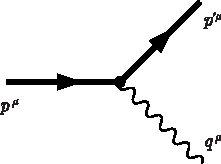
\includegraphics[width=0.5\linewidth]{intro-Compton-NL} 
  \end{minipage}
  \hfill
  \begin{minipage}[b][][b]{0.49\linewidth}\centering
      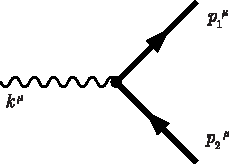
\includegraphics[width=0.5\linewidth]{intro-Breit-Wheeler-NL}
  \end{minipage}
  \caption{\fixme{Элементарные КЭД процессы во внешнем поле. (Добавить трайдент)}}
  \label{fig:intro/QED}
\end{figure}
Эти процессы являются экспоненциально подавленными при $\chi \lesssim 1$ и во многом аналогичны процессу образования электрон-позитронных пар по механизму Заутера-Швингера.
В силу того, что параметр $\chi$, помимо напряжённости ЭМ поля, определяется энергией частицы, ожидается, что экспериментальное наблюдение описанных таких процессов может быть возможным, например, на упомянутых выше лазерных установках нового поколения.
Однако, даже в режиме $\chi \lesssim 1$, когда образование электрон-позитронных пар подавлено, взаимодействие заряженных частиц с ЭМ полем может существенно изменяться за счёт реакции излучения.
Сам факт того, что заряженные частицы испытывают силу отдачи при излучении известен уже более века и изначально был описан в рамках классической электродинамики, однако привёл к противоречивости понятия об электроне как о точечном объекте и обозначил границу применимости классической ЭД, которую можно определить условием ${E_\mathrm{cl} = m^2 c^4 / e^3 = E_\mathrm{S} / \alpha}$.
Поле такой напряжённости создаёт электрон на расстоянии своего классического радиуса $r_e = e^2 / m c^2$.
Отметим, что оно в ${1/\alpha \approx 137}$ раз больше критического поля КЭД, поэтому квантовые эффекты появляются <<раньше>>, чем становится противоречивой классическая ЭД. 
Квантовая электродинамика описывает излучение фотонов электронами непротиворечивым образом и совпадает с результатами классической ЭД в пределе ${\chi\ll1}$.
Отдельный интерес, однако, представляет модификация спектра излучения и существенный эффект отдачи в режиме $\chi \gtrsim 1$, который практически не исследован экспериментально.
До недавнего времени существовал лишь единственный пример из 1990-х годов, а именно эксперимент E-144 на ускорителе SLAC \fixme{($a_0 \ll 1$, $\chi \ll 1$)}, где электронный пучок с энергией $\SI{46.6}{\giga\electronvolt}$ взаимодействовал с лазерным импульсом мощностью ${I\sim\SI{e18}{\watt/\centi\meter^2}}$, производя фотоны высокой энергии, которые, в свою очередь, превращались в электрон-позитронные пары в электромагнитном поле лазерного импульса~\cite{bula1996observation, burke1997positron}.
Недавно концептуально схожие  эксперименты были проведёны на установке Astra Gemini, где один лазерный импульс использовался для ускорения электронов, а второй~---~для рассеяния на ускоренных электронах~\cite{Poder17, Cole17} \fixme{($a_0 \sim 1$, $\chi \lesssim 1$)}.
Важно отметить, что несмотря на неоспоримую ценность этих экспериментов, их результаты содержат определённый уровень погрешности, который не позволяет с уверенностью заявлять о точности предсказаний КЭД.
Благодаря развитию технологий как лазерных установок, так и ускорителей, в ближайшем будущем ожидаются новые эксперименты по физике сильных полей, в частности прямой наследник эксперимента E-144~---~эксперимент E-320, на котором ожидается достижение существенно квантового режима взаимодействия~\cite{meuren2019probing} \fixme{($a_0 > 1$, $\chi > 1$)}.
Тем временем стремительно растёт число теоретических исследований, предсказывающих новые эффекты, вызванные влиянием реакции излучения на коллективные процессы.
Эти эффекты крайне различны и включают в себя, например, изменение механизмов ускорения частиц~\cite{Tamburini10, Tamburini12, kostyukov2012radiative, Capdessus12, Capdessus15, Nerush15, Gelfer18a, Gelfer18b, gelfer2021ions, golovanov2021radiation},
\fixme{радиационный захват частиц~\cite{Gonoskov14, Ji14b}}
крайне эффективное поглощение лазерного излучения~\cite{grismayer2016laser},
подавление релятивистской прозрачности~\cite{Zhang15, serebryakov2022opacity},
обратный эффект Фарадея~\cite{Liseykina16,liseykina2021IFE},
поляризацию частиц~\cite{DelSorbo2017Spin,DelSorbo2018spin,Chen2019spin,Seipt2019spin,Wu2019spin,li2019ultrarelativistic,Li2020spin,Wan2020spin,gong2021retrieving} и много других.

В режиме $\chi\gtrsim 1$ предполагается, что поведение вещества в экстремальных ЭМ полях в большом числе конфигураций во многом определяется развитием \textit{квантово-электродинамических каскадов}~\cite{nerush2007radiation,Bell2008,Nerush11a,Ridgers12,narozhny2015quantum,Kostyukov2016,grismayer2017seeded,jirka2017qed,luo2018qed,Yuan2018,del2018ion,Lu2018,Luo2018,efimenko2019laser}.
Суть КЭД каскада состоит в излучении жёстких фотонов ультрарелятивистскими частицами в результате нелинейного комптоновского рассеяния и последующий <<распад>> первых на электрон-позитронные пары в результате процесса Брейта-Уиллера\footnote{ Как было отмечено выше образование электрон-позитронной пары также возможно напрямую из электрона во внешнем в результате процесса Бете-Гайтлера}. 
Вторичные частицы также становятся вовлечены в образовании следующего поколения пар, что приводит к лавинообразному росту числа частиц.
Развитие таких каскадов качественно похоже на другой физический процесс~---~лавинообразную ионизацию при пробое в газе~\cite{raizer1997gas}.
Активное исследование микроволнового пробоя в газах выявило достаточно сложную динамику данного процесса, сопровождаемую образованием плазмы и генерацией волн пробоя~\cite{bollen1983high,semenov1982breakdown}.
Аналогия между рождением пар в вакууме и ионизацией газа, или между \textit{пробоем вакуума} в результате развития КЭД каскада и газового пробоя имеет глубокое физическое обоснование~\cite{dunne2012,narozhny2015quantum,efimenko2018extreme}.
Считается, что процессы развития КЭД каскадов играют немаловажную роль в различных астрофизических феноменах, таких как космические ливни~\cite{bhabha1937passage}, гамма-вспышки~\cite{meszaros2006gamma}, процессах в магнитосфере пульсаров~\cite{sturrock1971model,ruderman1975theory,daugherty1982electromagnetic, philippov2015ab} и др. 
Разнообразие и сложность образующихся в результате развития КЭД каскада структуры электрон-позитронной плазмы объясняет их активное исследование, далёкое от завершения.

Лабораторное моделирование астрофизических процессов (\textit{лабораторная астрофизика}) за счёт использования экстремально интенсивных лазеров является нетривиальной задачей с точки зрения постановки и интерпретации результатов эксперимента.
Во многом это связано с тем, что ключевую роль в астрофизических процессах играет взаимодействие потоков частиц друг с другом, поэтому для лабораторного моделирования таких процессов необходимо сначала создать такие потоки частиц с помощью лазера.
В этой связи, также исследуются альтернативные возможности, например, использование коллайдеров, являющихся основным инструментом исследований в области физики элементарных частиц, и которые основаны на лобовом столкновении пучков заряженных частиц высокой энергии.
В настоящее время существует несколько проектов, нацеленных на строительство высоко-энергетических лептонных коллайдеров с рекордными параметрами, таких как ILC~\cite{ILC} и CLIC~\cite{CLIC}.
Относительно недавно плазменное ускорение стало рассматриваться в качестве привлекательного альтернативного метода создания линейных коллайдеров с большим ускоряющим градиентом~\cite{schroeder2010physics}.
В области взаимодействия на таких коллайдерах могут генерироваться сильные ЭМ поля, благодаря чему возможно проявление таких эффектов, как \textit{разрушение} пучков (\textit{disruption})~\cite{hollebeek1981disruption,yokoya1992beam,chen1988disruption}, \textit{пучковое излучение} (\textit{beamstrahlung})~\cite{noble1987beamstrahlung,blankenbecler1987quantum,bell1995quantum}, образование вторичных электрон-позитронных пар~\cite{chen1989coherent,esberg2014strong}, и даже эффектов \textit{непертурбативной} сильнополевой КЭД~\cite{yakimenko2019prospect,tamburini2020efficient}.
Так как достижение всё больших интенсивностей излучения на лазерных установках предъявляет всё более жёсткие требования к контрасту, стабильности, качеству пучка, пока не достигнутые на практике~\cite{danson2019petawatt}, сильноточные высокоэнергетические коллайдеры, отличающиеся высоким качеством и стабильностью пучка, могут стать привлекательной <<безлазерной>> альтернативой для экспериментов в области физики сильного поля.
Наиболее активно в таком контексте обсуждается проект FACET-II, посвященный изучению плазменного ускорения~\cite{FACET, yakimenko2019prospect, del2019bright, meuren2019probing}.

Таким образом, исследование физики сильных полей представляет как фундаментальный интерес, так и практическое значение.

% \ifsynopsis
% Этот абзац появляется только в~автореферате.
% Для формирования блоков, которые будут обрабатываться только в~автореферате,
% заведена проверка условия \verb!\!\verb!ifsynopsis!.
% Значение условия задаётся в~основном файле документа (\verb!synopsis.tex! для
% автореферата).
% \else
% Этот абзац появляется только в~диссертации.
% Через проверку условия \verb!\!\verb!ifsynopsis!, задаваемого в~основном файле
% документа (\verb!dissertation.tex! для диссертации), можно сделать новую
% команду, обеспечивающую появление цитаты в~диссертации, но~не~в~автореферате.
% \fi

\vspace{0.25cm}
{\aim} данной работы является исследование влияния реакции излучения и образования электрон-позитронных пар на процессы, происходящие в экстремально сильных электромагнитных полях в различных конфигурациях, в частности при взаимодействии лазерного излучения с твердотельной мишенью, столкновении сильноточных пучков ультрарелятивистских частиц друг с другом и с плазменной мишенью.

Для~достижения поставленной цели были поставлены следующие {\tasks}:
\begin{enumerate}[beginpenalty=10000] % https://tex.stackexchange.com/a/476052/104425
  \item Разработать теорию движения отдельных заряженных частиц в сильных полях в режиме экстремальных радиационных потерь. Определить общие свойства движения частиц согласно разработанной модели. Применить теорию в различных конфигурациях электромагнитного поля. Определить область применимости модели, в частности путём сравнения полученных результатов с результатами, полученными численными методами.
  \item Исследовать взаимодействие лазерного импульса экстремальной интенсивности с твердотельной мишенью с помощью численного моделирования. Определить особенности и механизм развития квантово-электро\-динамического каскада при таком взаимодействии.
  \item Разработать аналитическую модель развития квантово-электро\-динамического каскада в поле плоской волны. Определить точность разработанной модели путём сравнения с результатами численного моделирования.
  \item Исследовать влияние реакции излучения на процесс фокусировки пучков ультрарелятивистских частиц при их лобовом столкновении. Разработать модель для вычисления параметра разрушения с учётом реакции излучения. Сравнить полученные аналитические результаты с результатами численного моделирования.
  \item Исследовать процесс генерации гамма-излучения при взаимодействии сильноточного пучка ультрарелятивистских электронов с плазменной мишенью с помощью численного моделирования. Разработать модели для вычисления эффективности конверсии энергии пучка в энергию гамма-излучения. Определить параметры пучка на установке FACET-II, оптимальные с точки зрения генерации гамма-излучения.
  \item Разработать численную схему решения уравнений Максвелла на сетке с подавленной черенковской неустойчивостью.
\end{enumerate}

\vspace{0.25cm}
{\novelty}
\begin{enumerate}[beginpenalty=10000] % https://tex.stackexchange.com/a/476052/104425
  \item Разработана асимптотическая теория движения заряженных частиц в режиме экстремальных радиационных потерь. Определены общие свойства движения частиц в таком режиме, существенно отличающиеся от таковых в режиме слабой реакции излучения. Продемонстрирован новый метод получения приближённого решения уравнений движения в различных конфигурациях.
  \item Обнаружен и качественно описан эффект развития самоподдерживающегося квантово-электродинамического каскада в поле, приближенном к полю плоской волны. Разработана аналитическая модель, описывающая развитие такого каскада.
  \item Разработана модель для вычисления параметра разрушения при лобовом столкновении сильноточных пучков ультрарелятивистских частиц с учётом реакции излучения. Достоверность модели подтверждена полноразмерным численным трёхмерным моделированием
  \item С помощью полноразмерного трёхмерного численного моделирования продемонстрирована схема эффективной генерации гамма-излучения при взаимодействии сильноточного пучка ультрарелятивистских электронов с протяжённой плазменной мишенью. Разработана аналитическая модель для вычисления эффективности конверсии энергии пучка в энергию гамма-излучения. Найдены параметры пучка для установки FACET-II, оптимальные с точки зрения генерации гамма-излучения.
  \item Разработана и реализована в коде QUILL альтернативная схема для численного решения уравнений Максвелла на регулярной сетке, отличающаяся существенно подавленной численной черенковской неустойчивостью, и подходящей для моделирования пучков ультрарелятивистских частиц.
\end{enumerate}

\vspace{0.25cm}
{\influence}
\begin{enumerate}[beginpenalty=10000]
  \item Разработанная теория движения частиц в условиях экстремальных радиационных потерь может быть использована в качестве дополнительного аналитического инструмента для определения динамики частиц в различных конфигурациях электромагнитного поля.
  \item Проведённое численное моделирование процесса взаимодействия экстремально интенсивного слабо-сфокусированного лазерного излучения с тонкой твердотельной мишенью расширяет класс конфигураций электромагнитного поля, в которых возможно наблюдение самоподдерживающегося квантово-электродинамического каскада.
  \item Разработанная аналитическая модель развития квантово-электро\-динамического каскада в плоской волне, учитывающая пространственную, а не только временную, динамику частиц может быть адаптирована для исследования развития квантово-электродинамических каскадов в других конфигурациях, например, при взаимодействии лазерного излучения с различными мишенями, пучками частиц, взаимодействие пучков друг с другом. 
  \item Проведённое численное моделирование и разработанная аналитическая модель усиления фокусировки сильноточных пучков при их столкновении за счёт реакции излучения может быть использована для уточнения требуемых параметров пучков при проведении экспериментов на коллайдерах и ускорителях нового поколения, таких как CLIC, ILC, FACET-II.
  \item Проведённое численное моделирование взаимодействия сильноточного пучка ультрарелятивистских частиц с протяжённой плазменной мишенью может быть использовано для планирования экспериментов на коллайдерах и ускорителях нового поколения по генерации яркого гамма-излучения. 
  \item Разработанная схема для численного решения уравнений Максвелла на сетке с подавленной черенковской неустойчивостью может быть реализована в PIC-кодах для существенного увеличения достоверности результатов моделирования процессов с участием пучков ультрарелятивистских частиц.
\end{enumerate}

% {\methods} \ldots

\vspace{0.25cm}
{\defpositions}
\begin{enumerate}[beginpenalty=10000] % https://tex.stackexchange.com/a/476052/104425
  \item Первое положение
  \item Второе положение
  \item Третье положение
  \item Четвертое положение
\end{enumerate}
% В папке Documents можно ознакомиться с решением совета из Томского~ГУ
% (в~файле \verb+Def_positions.pdf+), где обоснованно даются рекомендации
% по~формулировкам защищаемых положений.

\vspace{0.25cm}
{\reliability} полученных результатов обеспечивается использованием надёжных физических моделей и применением теоретических методов, имеющих строгое математическое обоснование, таких как теория возмущений,
разложение в ряд по малому параметру, усреднение по <<быстрому>> времени и др. 
Результаты сопоставлялась с результатами, полученными с помощью различных численных методов, в частности полномасштабного трехмерного численного моделирования, основанного на базовых физических принципах, а также с результатами, полученными ранее другими авторами.

\vspace{0.25cm}
{\probation}
Основные результаты диссертации докладывались на семинарах ИПФ РАН, а также на следующих конференциях, в том числе лично:
\begin{enumerate}
    \item XXII Научная конференция по радиофизике, Нижний Новгород, Россия, 2018;
    \item XXVIII Научная школа «Нелинейные волны 2018», Нижний Новгород, Россия;
    \item XXIII Научная конференция по радиофизике, Нижний Новгород, Россия, 2019;
    \item VII International Conference “Frontiers of Nonlinear Physics”, Nizhny Novgorod, Russia, 2019;
    \item XIX Научная школа «Нелинейные волны 2020», Нижний Новгород, Россия, 2020;
    \item IV International Conference <<UltrafastLight-2020>>, Moscow, Russia, 2020;
    \item ELI-NP Autumn School, Magurele, Romania, 2020;
    \item 20 международная конференция и молодёжная школа «Математическое моделирование и суперкомпьютерные технологии», Нижний Новгород, Россия, 2020;
    \item 63-я Всероссийская научная конференция МФТИ, Москва, Россия, 2020;
    \item The 2nd China-Russia Frontier Seminar on Ultra Intense Laser Technology and Intense Field Physics, Nizhny Novgorod, Russia, 2020;
    \item EPS 47th Conference on Plasma Physics, Sitges, Spain, 2021;
    \item 29th annual International Laser Physics Workshop, Lyon, France, 2021;
    \item V International Conference <<UltrafastLight-2021>>, Moscow, Russia, 2021;
    \item 18th International Workshop Complex Systems of Charged Particles and Their Interactions with Electromagnetic Radiation, Moscow, Russia, 2022;
    \item 30th annual International Laser Physics Workshop, Lyon, France, 2022.
\end{enumerate}

\vspace{0.25cm}
{\contribution} Основные положения, выносимые на защиту, отражают личный вклад автора в опубликованные работы.
Подготовка к публикации полученных результатов проводилась совместно с соавторами, причем вклад диссертанта был определяющим.
Все представленные в диссертации результаты получены лично автором.

\vspace{0.25cm}
{\publications} Основные результаты по теме диссертации изложены в~\total{citeauthor}~печатных изданиях, \total{citeauthorscopuswos} из которых изданы в~периодических научных журналах, индексируемых Web of~Science и Scopus~\autocite{artemenko2016formation, samsonov2018asymptotic, samsonov2019laser, samsonov2020superluminal, samsonov2021hydrodynamical, samsonov2021effect, samsonov2021beamstrahlung, filipovic2021effect, samsonov2022simulation, samsonov2022high}, \total{citeauthorconf} "--- в~тезисах докладов~\cite{samsonov2018NW, samsonov2019FNP, samsonov2020NW, samsonov2020UFL, samsonov2020Math, samsonov2021EPS, samsonov2021UFL, samsonov2021LPHYS, samsonov2022CSCPIER, samsonov2022LPHYS}.

% \begin{refsection}[bl-author]
% \end{refsection}

\begin{comment}
\ifnumequal{\value{bibliosel}}{0}
{%%% Встроенная реализация с загрузкой файла через движок bibtex8. (При желании, внутри можно использовать обычные ссылки, наподобие `\cite{vakbib1,vakbib2}`).
    {\publications} Основные результаты по теме диссертации изложены
    в~XX~печатных изданиях,
    X из которых изданы в журналах, рекомендованных ВАК,
    X "--- в тезисах докладов.
}%
{%%% Реализация пакетом biblatex через движок biber
    \begin{refsection}[bl-author]
        % Это refsection=1.
        % Процитированные здесь работы:
        %  * подсчитываются, для автоматического составления фразы "Основные результаты ..."
        %  * попадают в авторскую библиографию, при usefootcite==0 и стиле `\insertbiblioauthor` или `\insertbiblioauthorgrouped`
        %  * нумеруются там в зависимости от порядка команд `\printbibliography` в этом разделе.
        %  * при использовании `\insertbiblioauthorgrouped`, порядок команд `\printbibliography` в нём должен быть тем же (см. biblio/biblatex.tex)
        %
        % Невидимый библиографический список для подсчёта количества публикаций:
        % \printbibliography[heading=nobibheading, section=1, env=countauthorvak,          keyword=biblioauthorvak]%
        % \printbibliography[heading=nobibheading, section=1, env=countauthorwos,          keyword=biblioauthorwos]%
        % \printbibliography[heading=nobibheading, section=1, env=countauthorscopus,       keyword=biblioauthorscopus]%
        % \printbibliography[heading=nobibheading, section=1, env=countauthorconf,         keyword=biblioauthorconf]%
        % \printbibliography[heading=nobibheading, section=1, env=countauthorother,        keyword=biblioauthorother]%
        % \printbibliography[heading=nobibheading, section=1, env=countauthor,             keyword=biblioauthor]%
        % \printbibliography[heading=nobibheading, section=1, env=countauthorvakscopuswos, filter=vakscopuswos]%
        % \printbibliography[heading=nobibheading, section=1, env=countauthorscopuswos,    filter=scopuswos]%
        % %
        % \nocite{*}%
        %
        % {\publications} Основные результаты по теме диссертации изложены в~\arabic{citeauthor}~печатных изданиях,
        % \arabic{citeauthorvak} из которых изданы в журналах, рекомендованных ВАК\sloppy%
        % \ifnum \value{citeauthorscopuswos}>0%
        %     , \arabic{citeauthorscopuswos} "--- в~периодических научных журналах, индексируемых Web of~Science и Scopus\sloppy%
        % \fi%
        % \ifnum \value{citeauthorconf}>0%
        %     , \arabic{citeauthorconf} "--- в~тезисах докладов.
        % \else%
        %     .
        % \fi%

        {\publications} Основные результаты по теме диссертации изложены в~\total{citeauthor}~печатных изданиях, \total{citeauthorscopuswos} из которых изданы в~периодических научных журналах, индексируемых Web of~Science и Scopus~\cite{artemenko2016formation, samsonov2018asymptotic, samsonov2019laser, samsonov2021hydrodynamical, samsonov2021beamstrahlung, filipovic2021effect, samsonov2021effect, samsonov2022simulation, samsonov2022high}, \total{citeauthorconf} "--- в~тезисах докладов~\cite{samsonov2018NW, samsonov2019FNP, samsonov2020NW, samsonov2022LPHYS}.

        % \ifnum \value{citeregistered}=1%
        %     \ifnum \value{citeauthorpatent}=1%
        %         Зарегистрирован \arabic{citeauthorpatent} патент.
        %     \fi%
        %     \ifnum \value{citeauthorprogram}=1%
        %         Зарегистрирована \arabic{citeauthorprogram} программа для ЭВМ.
        %     \fi%
        % \fi%
        % \ifnum \value{citeregistered}>1%
        %     Зарегистрированы\ %
        %     \ifnum \value{citeauthorpatent}>0%
        %     \formbytotal{citeauthorpatent}{патент}{}{а}{}\sloppy%
        %     \ifnum \value{citeauthorprogram}=0 . \else \ и~\fi%
        %     \fi%
        %     \ifnum \value{citeauthorprogram}>0%
        %     \formbytotal{citeauthorprogram}{программ}{а}{ы}{} для ЭВМ.
        %     \fi%
        % \fi%
        % К публикациям, в которых излагаются основные научные результаты диссертации на соискание учёной
        % степени, в рецензируемых изданиях приравниваются патенты на изобретения, патенты (свидетельства) на
        % полезную модель, патенты на промышленный образец, патенты на селекционные достижения, свидетельства
        % на программу для электронных вычислительных машин, базу данных, топологию интегральных микросхем,
        % зарегистрированные в установленном порядке.(в ред. Постановления Правительства РФ от 21.04.2016 N 335)
    \end{refsection}%
    \begin{refsection}[bl-author]
        % Это refsection=2.
        % Процитированные здесь работы:
        %  * попадают в авторскую библиографию, при usefootcite==0 и стиле `\insertbiblioauthorimportant`.
        %  * ни на что не влияют в противном случае
        % \nocite{vakbib2}%vak
        % \nocite{patbib1}%patent
        % \nocite{progbib1}%program
        % \nocite{bib1}%other
        % \nocite{confbib1}%conf
        % \nocite{samsonov2020superluminal}
    \end{refsection}%
        %
        % Всё, что вне этих двух refsection, это refsection=0,
        %  * для диссертации - это нормальные ссылки, попадающие в обычную библиографию
        %  * для автореферата:
        %     * при usefootcite==0, ссылка корректно сработает только для источника из `external.bib`. Для своих работ --- напечатает "[0]" (и даже Warning не вылезет).
        %     * при usefootcite==1, ссылка сработает нормально. В авторской библиографии будут только процитированные в refsection=0 работы.
}
\end{comment}

% При использовании пакета \verb!biblatex! будут подсчитаны все работы, добавленные
% в файл \verb!biblio/author.bib!. Для правильного подсчёта работ в~различных
% системах цитирования требуется использовать поля:
% \begin{itemize}
%         \item \texttt{authorvak} если публикация индексирована ВАК,
%         \item \texttt{authorscopus} если публикация индексирована Scopus,
%         \item \texttt{authorwos} если публикация индексирована Web of Science,
%         \item \texttt{authorconf} для докладов конференций,
%         \item \texttt{authorpatent} для патентов,
%         \item \texttt{authorprogram} для зарегистрированных программ для ЭВМ,
%         \item \texttt{authorother} для других публикаций.
% \end{itemize}
% Для подсчёта используются счётчики:
% \begin{itemize}
%         \item \texttt{citeauthorvak} для работ, индексируемых ВАК,
%         \item \texttt{citeauthorscopus} для работ, индексируемых Scopus,
%         \item \texttt{citeauthorwos} для работ, индексируемых Web of Science,
%         \item \texttt{citeauthorvakscopuswos} для работ, индексируемых одной из трёх баз,
%         \item \texttt{citeauthorscopuswos} для работ, индексируемых Scopus или Web of~Science,
%         \item \texttt{citeauthorconf} для докладов на конференциях,
%         \item \texttt{citeauthorother} для остальных работ,
%         \item \texttt{citeauthorpatent} для патентов,
%         \item \texttt{citeauthorprogram} для зарегистрированных программ для ЭВМ,
%         \item \texttt{citeauthor} для суммарного количества работ.
% \end{itemize}
% Счётчик \texttt{citeexternal} используется для подсчёта процитированных публикаций;
% \texttt{citeregistered} "--- для подсчёта суммарного количества патентов и программ для ЭВМ.

% Для добавления в список публикаций автора работ, которые не были процитированы в
% автореферате, требуется их~перечислить с использованием команды \verb!\nocite! в
% \verb!Synopsis/content.tex!.
 % Характеристика работы по структуре во введении и в автореферате не отличается (ГОСТ Р 7.0.11, пункты 5.3.1 и 9.2.1), потому её загружаем из одного и того же внешнего файла, предварительно задав форму выделения некоторым параметрам

\vspace{0.25cm}
\textbf{Объем и структура работы.} Диссертация состоит из~введения,
\formbytotal{totalchapter}{глав}{ы}{}{},
заключения.
%% на случай ошибок оставляю исходный кусок на месте, закомментированным
%Полный объём диссертации составляет  \ref*{TotPages}~страницу
%с~\totalfigures{}~рисунками и~\totaltables{}~таблицами. Список литературы
%содержит \total{citenum}~наименований.
%
Полный объём диссертации составляет
\formbytotal{TotPages}{страниц}{у}{ы}{}, включая
\formbytotal{totalcount@figure}{рисун}{ок}{ка}{ков}.
Список литературы содержит
\formbytotal{citenum}{наименован}{ие}{ия}{ий}.    % Введение
\ifnumequal{\value{contnumfig}}{1}{\counterwithout{figure}{chapter}
}{\counterwithin{figure}{chapter}}
\ifnumequal{\value{contnumtab}}{1}{\counterwithout{table}{chapter}
}{\counterwithin{table}{chapter}}
\chapter{Общие свойства движения заряженных частиц в экстремально сильных электромагнитных полях}\label{ch:ch1}

\section{Введение}\label{sec:ch1/sec1}

\section{Асимптотическая теория движения заряженной частицы в условиях экстремальных радиационных потерь}\label{sec:ch1/sec2}
\section{Общие свойства асимптотических траекторий}\label{sec:ch1/sec3}
\section{Поправки высшего порядка к асимптотической теории}\label{sec:ch1/sec4}
\section{Применение асимптотической теории в различных конфигурациях электромагнитного поля}\label{sec:ch1/sec5}

If the amplitude of an optical field is such that an electron gains in it energy of hundreds of
its
rest-mass energy, the electron starts to emit synchrotron radiation and can lose its energy
efficiently~\cite{Bulanov04}. This phenomenon --- radiation reaction --- is highly important for theoretical physics
and astrophysics, therefore the motion of electrons in strong laser field nowadays is a topic of
numerous theoretical investigations~\cite{Di09, Duclous11, Nerush11b, Thomas12, Neitz13, Vranic16},
and it has been studied recently in the experiments~\cite{Cole17, Poder17}.  Also, the emission of
hard photons by electrons in a strong laser field lets one to make a femtosecond broadband source
of MeV photons, based on either laser pulse -- electron beam collision~\cite{Corde13, Sarri14,
Yan17}, laser-plasma interaction~\cite{Ridgers12, Bashinov13, Nerush14, JI14a, Li17} or
electromagnetic cascades~\cite{Nerush11a, Gonoskov17b}.

In the interaction of a strong laser pulse with a plasma, radiation losses can significantly
affect the plasma dynamics, and, for instance, lead to less-efficient ion
acceleration~\cite{Tamburini10, Tamburini12, Capdessus12, Capdessus15, Nerush15}, the enhancement of
the laser-driven plasma wakefield~\cite{Gelfer18a, Gelfer18b}, highly efficient
laser pulse absorption~\cite{Grismayer16}, relativistic transparency reduction~\cite{Zhang15}, and
to the inverse Faraday effect~\cite{Liseykina16}.

Despite of high importance of the radiation losses
for laser-plasma physics at high intensity, there is no general concept of the losses impact
on the electron motion, and this impact is considered mostly by \textit{ad hoc}
hypotheses and particle-in-cell (PIC) simulations.  Only for a few field configurations the
analytical solutions for motion of emitting electron are present~\cite{Zeldovich75, Di08a,
Kostyukov16a}, whereas for the motion of the non-emitting electron the Miller's ponderomotive
concept~\cite{Miller58} is applicable in a vast number of cases.

In the high-intensity field, the energy gained by the electron can be
significantly limited by the radiation losses. In this case, in contrast to the low-intensity
limit, the electron Lorentz factor becomes small in comparison with the field amplitude: $\gamma /
a_0 \ll 1$; here
$\gamma$ is the electron Lorentz factor and $a_0 = e E_0 / mc \omega$ is the normalized amplitude
of the electric field, $E_0$, $\omega$ is the typical angular frequency of the field, $c$ is the speed of
light, $m$ and $e>0$ are the electron mass and the magnitude of the electron charge, respectively.
The smallness of $\gamma / a_0$ allows one to simplify the analytical treatment of the electron motion
in the strong radiation-dominated regime. This can be illustrated by a stationary Zel'dowich's
solution~\cite{Zeldovich75} for the electron motion in the rotating electric field $\mathbf E(t)$. At
moderate field intensity the angle $\varphi$ (between the particle velocity and the vector
$-\mathbf E$) is
connected with the electron Lorentz factor $\gamma$. However, in the strong radiation dominated
regime $\varphi$ and $\gamma / a_0$ tend to zero (see Fig.), and the particle velocity
coincides with the direction
of the electric field ($\mathbf{v \parallel E}$), thus $\gamma$ is not needed in order to compute the particle trajectory.

In Refs.~\cite{Fedotov14b, Gonoskov17} the concept of the electron motion, that in the
radiation-dominated regime can supersede the ponderomotive concept, is discussed. It have been shown
in Ref.~\cite{Fedotov14b} that in the regime of dominated radiation friction the number of degrees
of freedom, which govern the electron motion, is reduced. Namely, it is shown for the rotating
electric field with the Gaussian envelope, that on the time scales larger than the rotation period,
the electron position is described by a first-order differential equation that does not contain the
electron momentum. For this, the electron motion with Landau--Lifshitz radiation reaction have been
considered. It is also shown that in the radiation-dominated regime,
electrons are not expelled from but are captured for a long time by the strong-field region.

% \begin{figure}
% 	\includegraphics[width=1\linewidth]{circe.pdf}
%     \caption{\label{circe}Electrons moving in the rotating electric field and experiencing quantum
%     radiation reaction for many periods of the rotation: (circles) the ratio of the mean Lorentz factor
%     $\gamma_m$ to $a_0$ and  (triangles) the
%     mean angle $\varphi_m$ between the particle velocity and the vector opposite to the electric field, for different
%     values of the field amplitude $a_0$. Bars depict the standard deviations $\pm \sigma$. Results
%     of PIC-MC simulations for the field angular frequency $\omega = 2 \pi c / \lambda$, $\lambda
%     = 1 \text{ } \mu \text{m}$.}
% \end{figure}

In Ref.~\cite{Gonoskov17} it is shown for almost arbitrary field configuration, that in the strong
field limit in a timescale, much smaller than the timescale of the field variation, the direction of the
electron velocity approaches some certain direction that is determined only by the values of the
local electric and magnetic fields. Then, as the electron velocity is known, the electron
trajectory can be reconstructed. This approach, called the ``low-energy limit'', was used (but not
described) for the fields of the linearly polarized standing waves earlier~\cite{Gonoskov14}.

Let us emphasize that if the electron velocity is determined not by the electron momentum but
by the local fields, one can describe the plasma dynamics with hydrodynamical equations. Indeed,
in this case the currents in the Maxwell's equations depend only on the particle density and
particle velocity (i.e. on the particle density and local EM fields), therefore the first-order
equation for the electron position together with the
Maxwell's equations and the continuity equation form a closed system of equations.

% In this paper we present the first step toward such a hydrodynamical approach to the plasma dynamics in
% the radiation-dominated regime. Namely, in Sec.~\ref{estimates} we estimate $\gamma / a_0$ ratio
% and the threshold of the radiation-dominated regime. In Sec.~\ref{Asymptote}
% for arbitrary field configuration we find the first-order equation for the electron position, by a
% method different from Ref.~\cite{Gonoskov17} and with B-case (see below)
% considered separately. The right-hand-side of this equation is the velocity field that is fully
% determined by the local field vectors.
% It is shown that $\gamma \ll a_0$ is enough for this first-order equation to be valid in the laser
% field.
% In Sec.~\ref{tests} we compare the solution of this first-order equation
% with the solution of the exact equations of the electron motion for a number of field configurations.
% In Sec.~\ref{absorption-induced-trapping} we discuss the relation between the velocity field and
% the Poynting vector. In
% Sec.~\ref{properties} the symmetry of the velocity field induced by the
% symmetry of the Maxwell's equations, is considered, and the dramatic difference between the
% ponderomotive description and the description by the velocity field in the radiation-dominated
% regime is demonstrated. Thus, in the subsection~\ref{standing-waves}, in the limit of strong fields, the electron motion
% in a wide class of periodic standing waves is shown to be periodic. From this, in the
% subsection~\ref{TE11} we show with a certain model of the laser beam that the beam
% can capture the electrons and carries them along itself with the beam group velocity.
% Sec.~\ref{conclusion} is the conclusion.

% \section{Strong radiation-dominated regime}
% \label{estimates}

% In order to estimate the threshold value of the normalized field amplitude $a_0$ for the
% radiation-dominated regime, let us start from
% the equations of the electron motion with the Landau--Lifshitz radiation reaction force
% incorporated:
% \begin{eqnarray}
%     \label{dpdt}
%     \frac{d\mathbf p}{dt} = -\mathbf E - \mathbf v \times \mathbf B - F_{rr} \mathbf v, \\
% 	\label{dgdt}
%     \frac{d\gamma}{dt} = -\mathbf v \mathbf E - F_{rr} v^2,
% \end{eqnarray}
% where time is normalized to $1/\omega$, $\mathbf v$ is the electron velocity normalized to the speed of light $c$, $\mathbf p =
% \gamma \mathbf v$ is the electron momentum normalized to $mc$, $\mathbf E$ and $\mathbf B$ are
% the electric and the magnetic fields respectively (normalized to $mc\omega/e$),
% and $F_{rr} \mathbf v$ is the main term of the radiation reaction force~\cite{LandauII}:
% \begin{equation}
%     \label{Frr}
%     F_{rr} = \alpha \gamma^2 \frac{2}{3} \frac{\hbar \omega}{mc^2} \left\{(\mathbf{E+v \times B})^2
%     - (\mathbf{Ev})^2 \right\}.
% \end{equation}
% Here $\alpha = e^2 / \hbar c \approx 1 / 137$ is the fine-structure constant and $\omega$ is the frequency characterizing the
% time-scale or the space-scale of the field (e.g. angular frequency of the laser field).

% The radiation losses increase sharply with the increase of $\gamma$, therefore for some electron Lorentz
% factor $\gamma = \bar \gamma$, the further energy gain stops due to the losses. The corresponding
% value $\bar \gamma$ can be found from Eq.~\eqref{dgdt} assuming that the transverse and the longitudinal
% to $\mathbf v$ components of the Lorentz force are of the order of $a_0$:
% \begin{equation}
%     \bar \gamma \approx \sqrt{\frac{3}{2 \alpha a_0} \frac{mc^2}{\hbar \omega}},
% \end{equation}
% where $a_0$ is the characteristic electric field strength.
% In the absence of the radiation reaction the electron energy in the field can be estimated as
% $\gamma \sim a_0$, thus the radiation-dominated regime corresponds to $\bar \gamma \ll a_0$ hence
% \begin{equation}
%     a_0 \gg a_0^* = \left(\frac{3}{2 \alpha} \frac{mc^2}{\hbar \omega} \right)^{1/3}.
% \end{equation}
% Note for the laser wavelength $\lambda = 1 \text{ }\mu\text{m}$ the amplitude $a_0^* \approx 440$ that
% corresponds to the intensity $I \approx 5 \times 10^{23} \text{ W}\, \text{cm}^{-2}$. This level of intensity is
% expected to be reached in the near future with such facilities as
% ELI-beamlines~\cite{Garrec14}, ELI-NP~\cite{ELI-NP}, Apollon~\cite{Apollon}, Vulcan 2020~\cite{Vulcan2020}, or
% XCELS~\cite{Bashinov14}.

% In the case of strong radiation losses the angle between the Lorentz force and the
% electron velocity can be small, and the transverse to $\mathbf v$ component of the Lorentz force
% becomes much lower than the longitudinal one. However, this doesn't affect much the given
% estimates. For instance, for the electron motion in the rotating electric field from the stationary
% Zel'dowich's solution~\cite{Zeldovich75} we get $\varphi
% \approx \gamma / a_0$ and $\gamma \approx (a_0 / \mu)^{1/4} \ll a_0$ (where $\mu = 2 \alpha \hbar \omega / 3
% mc^2$) at $a_0 \gg a_0^*$, with the same estimate for $a_0^*$ (except the factor $3/2$ in the
% parentheses, see Ref.~\cite{Zeldovich75}). Note also that the quantum consideration of the radiation reaction gives results that are
% close to the Zel'dovich's solution: in the Monte Carlo (MC) simulations the mean $\varphi$ value is about $\pi
% / 2$ times larger than $\gamma / a_0$, and $\gamma / a_0$ drops with the increase of the field
% amplitude (Fig.~\ref{circe}).

% In what follows we assume that the field is far beyond the threshold of the radiation-dominated
% regime, $a_0 \gg a_0^*$.

% \section{Velocity field and asymptotic trajectories}
% \label{Asymptote}

% The reduced equations of the electron motion for arbitrary field configuration can be derived as
% follows. The equation for the electron velocity can be obtained from Eqs.~\eqref{dgdt} and
% \eqref{dpdt}, and is the following:
% \begin{equation}
%     \label{dvdt}
%     \frac{d\mathbf v}{dt} = -\frac{1}{\gamma}\left\{ \mathbf{E - v (v E) + v \times  B} +
%     \frac{F_{rr} \mathbf v}{\gamma^2} \right\},
% \end{equation}
% where the first three terms in the parentheses approximately correspond to the transverse to $\mathbf v$
% component of the Lorentz force.

% If the angle $\psi$ between the Lorentz force and the electron velocity
% is noticeable
% ($\psi \sim 1$), then the term with
% $F_{rr}$ in Eq.~\eqref{dvdt} is negligible, because $F_{rr} / \gamma^2 \sim a_0^2 \alpha \hbar \omega /
% mc^2 \ll a_0$ for reasonable field amplitudes, $E_0 \lesssim E_S / \alpha$, where $E_S = m^2 c^3 / e
% \hbar$ is the Sauter--Schwinger critical field. Thus, as far as
% $\gamma \ll a_0$, we have $|d \mathbf v / dt|
% \gg 1$.

% It means that the characteristic timescale of the velocity vector variation is small,
% $\tau_{\mathbf v} \sim \gamma / a_0 \ll 1$. Therefore, on small time scales it can be assumed that the fields
% $\mathbf E$ and $\mathbf B$ in Eq.~\eqref{dvdt} are constant. In the constant EM field the
% electron velocity $\mathbf v$ in a time of some $\tau_{\mathbf v}$ approaches some asymptotic
% direction. This direction
% corresponds to $\psi \to 0$ hence $d \mathbf v / dt = 0$, and can be found as follows.

% \subsection{B-case}

% In the case $\mathbf{E \cdot B} = 0$ and $B > E$ there is a reference frame $K'$ in which the field
% is
% purely magnetic, and $\mathbf{B}' \parallel \mathbf{B}$ (here strokes denote quantities in $K'$).
% In $K'$ the electron goes along the helical path with its axis parallel to the
% direction of $\mathbf B'$. The corresponding drift velocity of the electron in the laboratory
% reference frame $K$ is the speed of $K'$ in $K$ and can be found from the following equation:
% \begin{equation}
% \label{eta}
% \mathbf{E + v \times B} = 0.
% \end{equation}
% Let us note that Eq.~\eqref{eta} does not depend on the component of the velocity parallel to the
% magnetic field,
% so one can choose this component arbitrarily (implying $v < 1$). One can choose, for example,
% the solution with $\mathbf{v \cdot B} = 0$, i.e.:
% \begin{equation}
% \label{eta_explicit}
%     \mathbf v = \frac{\mathbf{E \times B}}{B^2}.
% \end{equation}
% As shown in Sec.~\ref{TE11} the ambiguity of $\mathbf v$ in this case can be resolved by
% additional physical considerations.

% \subsection{E-case}

% If $E \cdot B \neq 0$ or $E > B$ there is a reference frame $K'$, in which $\mathbf{E'} \parallel
% \mathbf{B'}$ or $B' = 0$. The electron trajectory in $K'$ asymptotically approaches the straight
% line parallel to $\mathbf{E}'$, and $v$ approaches $1$. Note that for the resulting electron trajectory $\mathbf{ v
% \cdot E} < 0$ as far as the electron is accelerating by the field.

% As $v \approx 1$ and the electron moves along the straight line, in the laboratory reference frame
% $K$ the resulting $\mathbf v$ can be found from the equation $d\mathbf{v}/dt = 0$, that yields
% \begin{equation}
% \label{beta}
% \mathbf{E - v (v E) + v \times  B} = 0,
% \end{equation}
% Scalar multiplication of Eq. (\ref{beta}) by
% $\mathbf B$, $\mathbf E$ and $\mathbf{E \times B}$ leads to the following solution:
% \begin{eqnarray}
%     \label{betaB}
%     \mathbf{vB = \frac{EB}{vE}}, \\
%     \label{betaEB}
%     \mathbf{v \cdot E \times B} = E^2 - (\mathbf{v E})^2, \\
%     \label{betaE}
%     \mathbf{vE} = -\sqrt{\frac{E^2 - B^2 + \sqrt{(E^2-B^2)^2 +
%     4\mathbf{(EB)^2}}}{2}}, \\
%     \label{betaEEB}
%     \mathbf{v \cdot E \times [E \times B]} = \mathbf{(v E) (E B) -
%     (v B)} E^2.
% \end{eqnarray}
% The right-hand-side of Eq.~\eqref{betaE} is relativistic invariant, and we choose the sign ``$-$'' in
% order to obtain the stable trajectory in $K'$. For the opposite sign, ``$+$'', the electron in
% $K'$ is decelerating and its velocity is reversed quickly if initially $\mathbf v$ is not
% exactly parallel to the direction given by Eq.~\eqref{beta}. Note that vectors $\mathbf E$,
% $\mathbf{E \times B}$, $\mathbf{E \times [E \times B]}$ form an orthogonal basis thus
% Eqs.~\eqref{betaEB}--\eqref{betaEEB} are enough to determine $\mathbf v$ unambiguously.

% \subsection{Asymptotic trajectory}
% \label{Asymptote_c}

% Considering the electron motion on a timescale of the field variation timescale, $t \sim 1
% \gg \tau_{\mathbf v}$, one can neglect the dynamics of the electron while it is approaching the
% constant-field-approximation asymptotic solution, and assume that in every time instant the electron velocity
% is determined by Eq.~\eqref{eta} or Eq.~\eqref{beta} which depend only on the instant (and local) fields.
% Thus, the electron trajectory is governed by the following reduced-order equations:
% \begin{eqnarray}
% 	\label{r}
%      \frac{d\mathbf r}{dt} = \mathbf v, \\
% 	\label{v}
%     \mathbf{E - v (v E) + v \times  B} = 0,
% \end{eqnarray}
% where the last equation determines the velocity field $\mathbf v$ and can be used in both B- and
% E-cases (in B-case it yields Eq.~\eqref{eta}). From here on we call the solution of
% Eqs.~\eqref{r}--\eqref{v} ``asymptotic trajectory'' because, first, locally it corresponds to
% the asymptotic ($t \to \infty$) electron trajectory in the constant-field-approximation, and, second, it
% describes the electron trajectory in asymptotically strong field ($a_0 \gg a_0^*$).

% Note that the reasoning about the electron trajectory in the radiation-dominated regime is also
% valid if the parameter $\chi$ is large ($\chi \approx \gamma F_\perp / e E_s$,
% see Ref.~\cite{Berestetskii82, Elkina11}, where $F_\perp$ is the component of the Lorentz force perpendicular to
% the particle velocity). In this case ($\chi \gg 1$) the synchrotron emission is described by
% the quantum formulae and Eq.~\eqref{Frr} is not valid, however, it is still possible to describe the
% electron trajectory classically between the photon emission events~\cite{Baier98, Berestetskii82} because $\ell_f \ll \ell_W$. Here
% $\ell_f \sim mc^2 / F_\perp$ is the radiation formation length, i.e. the distance within which the emission of
% a single photon occurs, and $\ell_W \sim c / W$ is the mean distance that the electron passes
% without the photon emission; $W$ is the full probability rate of the photon emission. Estimating
% \begin{equation}
%     W \sim \frac{m c e^2}{\hbar^2} \frac{\chi^{2/3}}{\gamma},
% \end{equation}
% we obtain $\ell_f / \ell_W \sim \alpha / \chi^{1/3} < 1/137 \ll 1$.
% Therefore, the electron moves
% classically between the short events of the photon emission. Note also that for optical
% frequencies $\ell_W / \lambda \sim \hbar \omega / (\alpha \chi^{2/3} mc^2) \ll 1$.

% \section{Simple examples}
% \label{tests}

% In order to test the asymptotic description of the electron trajectory (Eqs.~\eqref{r} and \eqref{v}) we
% compare numerical solutions of them with numerical solutions of the classical equations of the
% electron motion with the radiation reaction taken into account by the inclusion of the
% Landau--Lifshitz force~\cite{LandauII} or
% by the recoil of the emitted photons described in the quasiclassical framework of
% Baier--Katkov~\cite{Berestetskii82, Baier98}.
% Numerical solution of the full equations of the electron motion is based on the Vay's
% pusher~\cite{Vay08} where the Landau--Lifshitz force is taken into account with the Euler's
% method or, alternatively,
% the quantum recoil is taken into account by 
% the Monte Carlo (MC) technique similarly to the QUILL~\cite{QUILL, Nerush17} code (see also
% Appendix~\ref{appendix-tests}). In order to
% solve Eqs.~\eqref{r}--\eqref{v} we use the classical Runge--Kutta method. The test results for
% various field configurations are present below.

% \subsection{Rotating electric field}

% In the rotating electric field of the amplitude $a_0$ Eq.~\eqref{v} gives $\mathbf{ v = -E} / E$,
% that coincides with the high-field limit ($a_0 \gg a_0^*$) of the Zel'dovich's stationary
% solution~\cite{Zeldovich75} utilizing the main term of the Landau--Lifshitz force. This stationary
% solution can be updated by taking into account quantum corrections to the radiation-reaction
% force~\cite{Bashinov17}, that also yields $\mathbf{v \to \mathbf -E} / E$ in the high-field limit.
% MC simulations demonstrate the same behavior, however, high dispersion of the angle between $\mathbf
% v$ and $\mathbf E$ is evident, see Fig.~\ref{circe}.

% \subsection{Static B-node}

% \begin{figure}
% 	\includegraphics[width=1\linewidth]{betafield.pdf}
%     \caption{\label{betafield}Velocity field Eq.~\eqref{v} (arrows) and the full electron trajectories in
%     the fields Eq.~\eqref{const_E_lin_B} for different values of the field magnitude: $a_0 = 500$
%     (dashed lines), $a_0 = 2 \times 10^3$ (dash-dotted lines) and $a_0 = 1 \times 10^4$ (solid
%     lines). The electrons start from $x_0 = \pm 0.3$ with its Lorentz factor $\gamma_0 = 100$ and
%     the momentum along $y$ axis.  The trajectories at $x < 0$ are computed with the Landau--Lifshitz
%     radiation reaction taken into account, while the trajectories at $x > 0$ are computed with
%     radiation reaction taken into account by Monte Carlo technique and quantum formulae
%     Eq.~\eqref{w}. Bars depict the standard deviation ($\pm \sigma$) of the final electron position
%     computed with 400 trajectories. The coordinates are normalized to $1/k = \lambda / 2 \pi$,
%     where $\lambda = 1 \text{ }\mu \text{m}$.}
% \end{figure}

% Let us start from the following simple field configuration:
% \begin{equation}
%     \label{const_E_lin_B}
%     E_y = a_0, \quad B_z = a_0 x,
% \end{equation}
% and the other components of the fields are zero.

% In Fig.~\ref{betafield} the velocity field Eq.~\eqref{eta_explicit} ($|x| > 1$) and Eqs.~\eqref{betaEB} and
% \eqref{betaE} ($|x| \leq 1$) is depicted by the arrows.
% In the left half of Fig.~\ref{betafield} the electron trajectories computed with the
% Landau--Lifshitz
% force are shown, and in the right half of Fig.~\ref{betafield} the electron trajectories are
% computed with Monte Carlo technique and quantum synchrotron formulae. Obviously, the shape of the electron trajectories computed
% with Monte Carlo approach is slightly different for different runs, so the bars depict the standard deviation of
% the electron final position. The trajectories are computed for different $a_0$ values, namely $a_0
% = 500$, $2 \times 10^3$, $1 \times 10^4$ which correspond to dashed, dash-dotted and solid lines,
% respectively. First, it is seen that at higher $a_0$ values the real electron velocity coincides
% better with the velocity field that induces the asymptotic trajectories. Second, the
% Landau--Lifshitz approach
% demonstrate slightly better coincidence, because in the Landau--Lifshitz approach the mean electron energy generally
% less than in the quantum approach.

% Note that the fields Eq.~\eqref{const_E_lin_B} resemble the $B$ node of a standing linearly polarized
% wave, however, in the linearly polarized standing wave the sign of $\mathbf{E \times B} |_x$ varies
% in time, and the node
% attracts the asymptotic electron trajectories during a half of a period, and repels them during the other
% half.

% \subsection{Linearly polarized standing wave}

% In the linearly polarized standing wave asymptotic electron trajectories can be found analytically.
% The fields of the linearly polarized standing wave read as follows:
% \begin{eqnarray}
%     \label{lpE}
%     \mathbf E = \mathbf{y_0} a_0 \cos (t) \cos (x), \\
%     \label{lpB}
%     \mathbf B = \mathbf{z_0} a_0 \sin (t) \sin (x),
% \end{eqnarray}
% where $\mathbf y_0$ and $\mathbf z_0$ are the unit vectors along the $y$ and $z$ axes,
% respectively.
% Then from Eqs.~\eqref{eta_explicit}, \eqref{betaEB} and \eqref{betaE} we get:
% \begin{equation}
% \mathbf v = \begin{cases}
% \mathbf{x}_0 \tan (t) \tan (x) \pm \mathbf{y}_0 \sqrt{1-\tan^2(t) \tan^2(x)}, & E>B \\
% \mathbf{x_0} \cot (t) \cot (x), & E<B.
% \end{cases}
% \end{equation}

% Since the fields are homogeneous along the $y$ axis electron's motion along it is not of any interest.
% Then $x(t)$ of the asymptotic trajectory is found from the following algebraic equations:
% \begin{equation}
% \label{xt_lpw}
% \begin{cases}
% \sin (x) \cos(t) = \sin (x_0) \cos (t_0), & E>B \\
% \cos (x) \sin(t) = \cos (x_0) \sin (t_0), & E<B.
% \end{cases}
% \end{equation}
% where the starting point $x_0 = x(t_0)$ also belongs to the region $E > B$ or $E < B$. For
% instance, the electron trajectory initially is determined by the first of Eqs. (\ref{xt_lpw}), then it reaches the point
% with $E=B$; after that the trajectory is determined by the second of Eqs. (\ref{xt_lpw}) up to the
% moment when the electron reaches another point with $E=B$ and so on.
% For $E = B$ Eqs.~\eqref{lpE} and \eqref{lpB} yields
% \begin{equation}
%     \label{E=B}
%     |\tan(x)\tan(t)| = 1
% \end{equation}
% with the following solution:
% \begin{equation}
%     x = \pm t + \frac{\pi}{2} + \pi n, \quad n = 0, \pm 1, \pm 2, ...
% \end{equation}

% For the electron starting from the point $x_0$ at the moment $t_0=0$ the chain of points $(x_1,
% t_1), \; (x_2, t_2), ...$ at which $E = B$ is the following. First, from Eqs.~\eqref{xt_lpw} and
% \eqref{E=B} under
% the assumption that initially $E > B$, we have:
% \begin{equation}
% \cot x_1 = \tan t_1 = \sqrt{\frac{1}{\cos (x_0)} - 1}
% \end{equation}
% The coordinate $x_2$ can be found from the observation that $x_2 = x_1$ and $t_2 = \pi - t_1$ obey
% the second of Eqs.~\eqref{xt_lpw} with $x_0$, $t_0$ replaced by $x_1$, $t_1$. Also, $x_2 = x_1$ and
% $t_2 = \pi - t_1$ obey Eq.~\eqref{E=B} (because $x_1$ and $t_1$ obey them).
% Analogously, $x_3 = x_2$ and $t_3 = \pi + t_1$. Then the electron trajectory periodically repeat
% itself (see Fig.~\ref{onion} (a)).

% \begin{figure}
%     \includegraphics[width=1\linewidth]{onion.pdf}
%     \caption{\label{onion} The electron motion (a), (b) in the field of the linearly polarized standing
%     electromagnetic wave Eqs.~\eqref{lpE}--\eqref{lpB} and (c) in the field of two counter-propagating linearly
%     polarized waves with a plane at $x = 0$ absorbing 70\% of the incoming energy (see
%     Eqs.~\eqref{lpaE}--\eqref{lpaB}, $R = 0.55$). Pale lines depict asymptotic trajectories
%     obtained by
%     the numerical integration of Eqs.~\eqref{r} for the E- and B-cases (solid thin beige line and
%     dotted blue line, respectively).
%     Dark thick lines correspond to the numerical
%     integration of the classical electron motion equations with quantum radiation
%     reaction~\eqref{w} taken into account by Monte Carlo technique, for $a_0 = 1\times 10^3$ and
%     $a_0 = 1 \times 10^4$ (starting at $x < 0$ and $x > 0$, respectively). It is worth to mention that the
%     pale
%     lines in (a) coincides with the analytical solution Eq.~\eqref{xt_lpw} and with the thin green lines
%     in Fig.~2 from Ref.~\cite{Gonoskov14}.}
% \end{figure}

% Note that the electron trajectory in the linearly polarized standing wave is periodic in
% the framework of the presented asymptotic theory. As shown in Sec.~\ref{standing-waves}, this is just an example
% of the general behaviour of the electron trajectories in standing waves in the radiation-dominated
% regime. However, it can seem that this
% behavior contradicts the anomalous radiative trapping~\cite{Gonoskov14} (ART). Really, ART
% is caused by a drift of the electron between the asymptotic
% trajectories given by Eqs.~\eqref{xt_lpw}. This drift takes many periods of the
% field~\cite{Gonoskov14} and can not be described by the presented asymptotic theory.

% The asymptotic electron trajectories computed with Eqs.~\eqref{r} and \eqref{v} are shown in
% Fig.~\ref{onion} (a) with thin pale dotted and solid lines (the computed trajectories coincide exactly
% with the analytical solutions Eqs.~\eqref{xt_lpw}). Six electron trajectories computed with Vay's
% pusher and Monte Carlo technique for the photon emission are also depicted: for $a_0 = 1 \times 10^3$ by
% green lines (starting at $x < 0$), and for $a_0 = 1 \times 10^4$ by red lines (starting at $x < 0$). Fig.~\ref{onion} (b) shows the energy of the
% electrons on the trajectories A and B from Fig.~\ref{onion} (a). The coincidence of the electron
% trajectories computed for $a_0 = 1 \times 10^4$ with the asymptotic trajectories are evident,
% opposite to $a_0 = 1 \times 10^3$ case in that the condition $\gamma \ll a_0$ is not fulfilled.
% Note that in the case of $a_0 = 1 \times 10^4$ the electrons moving according to the MC approach to
% the radiation reaction, become closer to the
% B-nodes for each subsequent period, that is the effect of ART.

% \section{Absorption-induced trapping}
% \label{absorption-induced-trapping}

% It follows from Eqs.~\eqref{eta_explicit} and \eqref{betaEB} that the angle between the asymptotic velocity
% $\mathbf v$ and the Poynting vector $\mathbf{ S \propto E \times B}$ is always less than $\pi /
% 2$, i.e. $\mathbf{ v \cdot S} > 0$. This hints that the electron motion in the radiation-dominated
% regime can be connected with the energy flow of the electromagnetic fields. Let us
% consider the region containing currents which (partially) absorb the incoming electromagnetic wave.
% In the average, the Poynting vector is directed into the region of the currents, and we suggest that
% in the radiation-dominated regime this region attracts the electron trajectories.
% In this section we verify this suggestion in a couple of examples.

% A plane wave pushes initially immobile electrons approximately in the direction of the Poynting
% vector, so it can seem that the absorption-induced trapping can be realized without strong radiation
% reaction. However, as seen from the examples below, in the absence of strong radiation losses if the
% electrons have been accelerated by a wave, then they can not be turned back by a counter-propagating
% wave. Thus the radiation reaction may cause electron trapping in the region with strong absorption
% of the electromagnetic energy.

% \subsection{Counter-propagating linearly polarized waves partially absorbing by a plane}

% The field of two counter-propagating linearly polarized (along the $y$ axis) waves, that is
% partially absorbing at the
% plane $x = 0$, can be written as follows:
% \begin{eqnarray}
%     \label{lpaE}
%     \mathbf E = \mathbf{y_0} a_0 \left\{ \cos (t) \cos (x) - 0.5 (1 - R) \cos(x \mp t) \right\}, \\
%     \label{lpaB}
%     \mathbf B = \mathbf{z_0} a_0 \left\{ \sin (t) \sin (x) \mp 0.5 (1 - R) \cos(x \mp t) \right\},
% \end{eqnarray}
% where in $\mp$ the upper sign corresponds to $x > 0$ and the lower one corresponds to $x < 0$, and
% $R$ is the reflection coefficient. The asymptotic and Vay+MC electron trajectories in this field are shown in
% Fig.~\ref{onion} (c) with the same color codes as in Fig.~\ref{onion} (a). Here $R = 0.55$ that
% means absorption of $70 \%$ of the wave energy in the plane $x = 0$. As seen from the figure, the
% electron trajectories are attracted by the plane $x = 0$ in the strong radiation-dominated regime, whereas
% at moderate intensity of the waves the electrons easily pass the plane. The mean standard
% deviation of $x$ computed for the Vay+MC electron trajectories for ten periods of the wave and $x_0 =
% 0.25 \lambda$ is about
% $1.5 \lambda$ for $a0 = 1 \times 10^3$ and $0.2 \lambda$ for $a_0 = 1 \times 10^4$.

% \subsection{Multipole wave absorbing by a current loop}

% \begin{figure}
% 	\includegraphics[width=1\linewidth]{currentloop.pdf}
%     \caption{\label{currentloop} (a) The magnetic field of a multipole wave that is entirely
%     absorbing by a current loop (see App.~\ref{appendix-multipole-wave}), the loop radius is $r_\ell = \lambda = 1 \text{ } \mu
%     \text{m}$, $t = 0$. The axis of the loop coincides with the $z$ axis and the position of a ``wire''
%     is shown by the black cross. (b) Asymptotic electron trajectories for E- and B-case (solid beige and
%     dotted blue, respectively) in the multipole wave. The electrons start to move at $t = 0$ from the
%     points on the circle $(r^2 + z^2)^{1/2} = 1.5 \, r_\ell$ (thick black dashed line).
%     The Vay+MC electron trajectories in the field of the multipole wave for (c) $I_0 = 1 \times
%     10^3$ and (d) $I_0 = 5 \times 10^3$. All trajectories are computed for $t \in [0, 5 \lambda /
%     c]$.}
% \end{figure}

% The field of a multipole harmonic wave that is completely absorbing by a current loop can be obtained
% by time reversal of the field emitting by a current loop (see
% App.~\ref{appendix-multipole-wave}). The
% electron motion in the absorbing multipole wave with the angular frequency $\omega = 2 \pi c / \lambda$
% for a loop radius $r_\ell = \lambda = 1 \; \mu \text{m}$ is shown in Fig.~\ref{currentloop},
% where in the cylindrical coordinate system the ``wire'' position is marked with the black cross.
% The $z$ axis is the axis of the loop.
% Fig.~\ref{currentloop} (a) demonstrates the magnetic field of the multipole wave at $t = 0$. Fig.~\ref{currentloop} (b)
% shows the asymptotic electron trajectories, Figs.~\ref{currentloop} (c) and (d) show the electron
% trajectories computed by Vay+MC
% algorithm for the loop current magnitude $I_0 = 1 \times 10^3$ and for
% $I_0 = 5 \times 10^3$, respectively. The trajectories start at $t = 0$ from the sphere shown by a thick dashed
% line and are computed up to $t = 5 \lambda / c$. 

% In the region very close to the ``wire'' the field gradient is huge hence the scale of the field
% change can be less than the radiation formation length. Thus, strictly speaking, more accurate
% consideration of the radiation reaction near the ``wire'' should be used. However, as discussed in
% Sec.~\ref{Asymptote_c}, it does not generally matter that exact form of the radiation reaction is
% used, because for the asymptotic description to be valid it is enough that the electron Lorentz
% factor is small in comparison with the field amplitude.

% It is seen from Fig.~\ref{currentloop} that the current loop attracts the asymptotic electron
% trajectories. However, it is seen that the absorption-induced trapping is not really a strict
% trapping but just means that electrons in the radiation-dominated regime stay for a long time in
% the region with the currents absorbing the incoming waves.

% \section{Emission-absorption symmetry and general properties of asymptotic trajectories}
% \label{properties}

% In this section we consider the properties of the electron trajectories described by Eqs.~\eqref{r}
% and \eqref{v}. For this purpose let us consider the well-known symmetry of the Maxwell's equations,
% namely, the following transform
% \begin{eqnarray}
%     \label{symmetry_t}
%     t^* = - t, \\
%     \label{symmetry_E}
%     \mathbf{E^* = -E}, \\
%     \label{symmetry_B}
%     \mathbf{B^* = B}, \\
%     \label{symmetry_j}
%     \rho^* = -\rho, \qquad \mathbf{j^* = j}.
% \end{eqnarray}
% does not change them, i.e. they leads to the Maxwell's equations for the starred variables; here
% $\rho$ is the charge density and $\mathbf j$ is the current density. From
% here on we denote $\mathbf{E}$, $\mathbf{B}$, $\mathbf{j}$ evolving in time $t$ as {\it initial}
% system and $\mathbf{E}^*$, $\mathbf{B}^*$, $\mathbf{j}^*$ evolving in time $t^*$ as {\it starred}
% system. This symmetry is the relation between a system of currents emitting some fields and the
% system of currents absorbing the fields: namely, the Poynting vector, the $\mathbf{j \cdot E}$
% product and the time direction in the starred system is opposite to that in the initial system.

% According to~Eq.~\eqref{v}, in the starred system the velocity field $\mathbf{v}^*$ relates to the velocity
% field of the initial system $\mathbf{v}$ as follows:
% \begin{equation}
%     \label{symmetry_v}
%     \mathbf{v}^*(\mathbf{r}, t^*) = -\mathbf{v(\mathbf{r}, -t^*)},
% \end{equation}
% that obeys the stability condition $\mathbf{v^* \cdot E^*} < 0$. Thus, in the starred system
% the velocity field and the time direction are opposite to that in the initial system, that
% leads to the same trajectories in the starred system $\mathbf{r}^*(t^*)$ as in the initial system,
% passed by the electrons in the opposite direction:
% $d \mathbf{r}^* / dt^* = \mathbf{v}^*(\mathbf{r}^*, t^*) = -\mathbf{v}(\mathbf{r}^*, -t^*)$.

% Let us note a fundamental difference between the asymptotic trajectories described by Eqs.~\eqref{v}, \eqref{r},
% and by the ponderomotive description.
% The ponderomotive force is determined by the distribution of $E^2$ and $B^2$ and is
% indifferent to the transform Eqs.~\eqref{symmetry_t}--\eqref{symmetry_j}, whereas this transform reverses
% the direction of the electron motion in the case when Eqs.~\eqref{v} and \eqref{r} are applicable,
% namely, when radiation reaction is strong.

% In order to illustrate the difference between the ponderomotive description and the description by
% the velocity field Eq.~\eqref{v} the following toy example can be considered. An electron is
% scattered by two compact counter-propagating laser pulses initially separated by some distance. The
% first one propagates, say, along the direction $\mathbf{x}_0$ and the second pulse is formed from
% the first one with the substitution~\eqref{symmetry_t}--\eqref{symmetry_B}, thus it propagates in
% the direction $-\mathbf{x}_0$. We suppose that the electron initially is closer to the first laser
% pulse that hence scatters the electron aside (if we consider the task in the framework of the
% ponderomotive description). In this case the electron can move far away from the pulses and the
% field of the second laser pulse is then unimportant. However, if the radiation reaction is strong,
% the asymptotic approach should be valid. In this case the trajectory of the electron in the field
% of the second laser pulse is the same as in the field of the first one but the electron passes the
% trajectory in the opposite direction (see Eq.~\eqref{symmetry_v}). Therefore in the
% radiation-dominated regime, the electron after its motion in the field of the first laser pulse
% will be brought back to its initial position by the second laser pulse that differs strongly from
% that the ponderomotive approach predicts.

% Thus, the asymptotic description of the electron motion~Eqs.~\eqref{r} and \eqref{v} implies that
% the electrons are not scattered by, but stay for a long time in the field of a laser pulse or in a
% laser beam. This conclusion is in a good agreement with the results of theoretical considerations
% and numerical simulations showing that the ponderomotive force can be significantly suppressed by the
% radiation reaction~\cite{Fedotov14b, Ji14b}.

% \subsection{Asymptotic trajectories in standing waves}
% \label{standing-waves}

% We see in Sec.~\ref{tests} that the reduced equations lead to periodic electron trajectories in
% the linearly polarized standing electromagnetic wave.
% Here we show, that Eqs.~\eqref{r} and \eqref{v} always lead to a periodic electron trajectories in a
% wide class of fields, namely in the \textit{periodic} fields which can be represented in the following form:
% \begin{eqnarray}
%     \label{Esw}
%     \mathbf{E} = \mathbf{f}(\mathbf{r}, t) - \mathbf{f}(\mathbf{r}, -t), \\
%     \label{Bsw}
%     \mathbf{B} = \mathbf{g}(\mathbf{r}, t) + \mathbf{g}(\mathbf{r}, -t),
% \end{eqnarray}
% where $\mathbf{E = f}(\mathbf{r}, t)$, $\mathbf{B = g}(\mathbf{r}, t)$ is the solution of Maxwell's
% equations for some charge density $\rho$ and current density $\mathbf{j}$ (for the sake of simplicity let
% us consider $\rho = 0$ and $\mathbf{j} = 0$). This representation
% means that the fields are the sum of the fields of some system and the fields of the corresponding
% starred system. In this case the symmetry \eqref{symmetry_t}--\eqref{symmetry_j} leads to the same
% fields of the starred system as in the initial system, i.e. $\mathbf{E}^*(\mathbf{r}, t^*) = \mathbf{E}(\mathbf{r}, t^*)$, $\mathbf{B}^*(\mathbf{r}, t^*)
% = \mathbf{B}(\mathbf{r}, t^*)$, hence it should lead to the same
% velocity field $\mathbf{v}^*(\mathbf{r}, t^*) = \mathbf{v}(\mathbf{r}, t^*)$, that together with
% Eq.~\eqref{symmetry_v} yields
% \begin{equation}
%     \mathbf{v}(\mathbf{r}, -t) = -\mathbf{v(\mathbf{r}, t)}.
% \end{equation}
% Thus, the velocity field in the electromagnetic fields~\eqref{Esw}--\eqref{Bsw} is an odd function of
% time. Consequently, the time reversal conserves the equation for the electron position,
% \begin{equation}
%     \frac{d \mathbf{r}}{d(-t)} = \mathbf{v}(\mathbf{r}, (-t)),
% \end{equation}
% and the electron position $\mathbf{r}(t)$ is an even function of time. Therefore,
% \begin{multline}
%     \mathbf{r}(t) - \mathbf{r}(-t) = \int_{-t}^t \mathbf{v}(\mathbf{r}(t), t) \, dt = \\
%     \int_{0}^t \mathbf{v}(\mathbf{r}(t), t) \, dt + \int_{0}^t \mathbf{v}(\mathbf{r}(-t), -t) \, dt
%     = 0.
% \end{multline}

% As far as the velocity field governed by Eqs.~\eqref{eta_explicit} and \eqref{betaB}--\eqref{betaEEB} is
% a single-valued function of the electromagnetic fields, and the fields are periodic in time, the
% velocity field is also periodic with the same period, $T$. Thus, the velocity field is an odd
% function relative to any
% time instant $t = n T$, where $n$ is an integer. Let the electron starts to move at $t = nT - T /
% 2$, then it comes to the starting point a period later, $\mathbf{r}(nT + T / 2) = \mathbf{r}(nT - T /
% 2)$, then due to the periodicity of $\mathbf{v}$ at $t = (n + 1) T$, we have $\mathbf{r}((n + 1)T + T /
% 2) = \mathbf{r}(nT + T / 2)$. Therefore, in the framework of the asymptotic approach, the electron is moving periodically back and forth along
% the same path in the periodic fields Eqs.~\eqref{Esw}--\eqref{Bsw}.

% \subsection{Asymptotic trajectories in a laser beam of finite diameter}
% \label{TE11}

% \begin{figure*}
%     \centering
% 	\includegraphics{te11.pdf}
%     \caption{\label{te11}(a) The electric and magnetic fields (red and blue arrows, respectively;
%     the electric field is mostly horizontal) of the continued TE11 mode of a
%     waveguide, Eqs.~\eqref{te11-2}--\eqref{te11-3} and \eqref{te11-5}--\eqref{te11-6}, at $t = 0$.
%     (b) The asymptotic
%     trajectory of an electron computed with Eqs.~\eqref{r}, \eqref{eta_explicit} and
%     \eqref{betaB}--\eqref{betaEEB} in the laboratory reference frame; $\xi = x - v_g t$, where
%     $v_g$ is the group velocity of the TE11 mode.
%     (c) The same asymptotic trajectory (dark thick line) and typical electron trajectories starting
%     at the point $x = 0$, $y = 0.2 \, \lambda$, $z = 0.65 \, \lambda$ ($\lambda = 1
%     \text{ } \mu \text{m}$, $t \in [0, 2 \tau]$), for $a_0 = 700$ (solid thin green line) and $a_0 = 4 \times
%     10^3$ (dotted red line).}
% \end{figure*}

% Here we stress that many field configurations could be reduced to the form
% of periodic fields that obey the emission-absorption symmetry
% Eqs.~\eqref{symmetry_t}--\eqref{symmetry_j}. In the previous subsection we also assumed that the
% velocity field is a single-valued function of the fields. This is not strictly true in the B-case,
% because one can add to $\mathbf{v}$ from Eq.~\eqref{eta_explicit} a vector parallel to $\mathbf{B}$.
% The effect of this ambiguity is also discussed in this section.

% Let us consider the fields of TE11 mode of a rectangular metallic waveguide:
% \begin{eqnarray}
%     \label{te11-1}
%     E_x = 0, \\
%     \label{te11-2}
%     E_y = a_0 \cos(k_y y) \sin(k_z z) \cos(t - k_x x), \\
%     \label{te11-3}
%     E_z = -\frac{a_0 k_y}{k_z} \sin(k_y y) \cos(k_z z) \cos(t - k_x x), \\
%     \label{te11-4}
%     B_x = \frac{a_0 (k_z^2 + k_y^2)}{k_z} \cos(k_y y) \cos(k_z z) \sin(t - k_x x), \\
%     \label{te11-5}
%     B_y = -k_x E_z, \\
%     \label{te11-6}
%     B_z = k_x E_y,
% \end{eqnarray}
% where we assume that the wave angular frequency $\Omega = (k_x^2 + k_y^2 + k_z^2)^{1/2}
% = 1$ (here we use the normalization frequency $\omega$ equal to the frequency of the wave, and, as before, the
% time is normalized to $1/\omega$, coordinates are normalized to $c / \omega$, $\mathbf k$ is the
% wavenumber normalized to $\omega / c$).
% These fields obey the metallic boundary conditions at $y = 0, \; \pm \ell_y, \; \pm 2 \ell_y,...$
% ($E_z = 0$) and at $z = 0, \; \pm \ell_z, \; \pm 2 \ell_z,...$ ($E_y = 0$). Here $\ell_y = \pi /
% k_y$ and $\ell_z = \pi / k_z$ are the sizes of the waveguide along the $y$- and $z$-axes,
% respectively.

% The fields Eqs.~\eqref{te11-1}--\eqref{te11-6} are the solution of the Maxwell's equations not only inside the waveguide but in
% the open space as well because this fields can be represented as a sum of plane waves. Particularly, we consider these fields in the region $y \in [-\ell_y / 2, \ell_y /
% 2]$ and $z \in [0, \ell_z]$ as the model of the laser beam of finite diameter. If $\ell_y \gg
% \ell_z$, the electric field is mainly directed along the $y$-axis and reaches its maximum in the
% center of the beam.

% The fields Eqs.~\eqref{te11-1}--\eqref{te11-6} are shown
% in Fig.~\ref{te11} (a) for $\ell_y = 4 \pi$, $\ell_z = 2 \pi$ and $t = x = 0$. The asymptotic electron
% trajectory computed for these fields is shown in Fig.~\ref{te11} (b), where $\xi = x - v_g t$, $v_g
% = k_x \approx 0.83$ is the group velocity of the electromagnetic wave, and the trajectory starts at
% $t = 0$, $x = 0$, $y = 0.2$ and $z = 0.65$ and is computed up to $t = 2 \tau$, where
% \begin{equation}
%     \label{tau}
%     \tau = \frac{2 \pi}{k_x (v_\phi - v_g)} = \frac{2 \pi}{1 - k_x^2}
% \end{equation}
% is the intrinsic timescale of the task, $v_\phi = 1 / v_g$ is the phase
% velocity of the wave. For Fig.~\ref{te11} $c \tau / \lambda \approx 3.2$.
% In Figs.~\ref{te11} (c) and (d) the same asymptotic trajectory is shown as the thick blue line. Five
% electron trajectories in the fields given by Eqs.~\eqref{te11-1}-\eqref{te11-6} are shown in Figs.~\ref{te11}
% (c) and (d). These trajectories start at the same point as the asymptotic trajectory, but they are
% computed by Vay's algorithm with quantum radiation reaction incorporated by Monte Carlo technique.
% For Figs.~\ref{te11} (c) and (d) we use $a_0 = 700$ and $a_0 = 4 \times 10^3$, respectively.

% It is seen from Figs.~\ref{te11} (b), (c) and (d) that the asymptotic trajectory is quasiperiodic,
% that is in a qualitative agreement with the fact that
% for $a_0 = 4 \times 10^3$ the electrons stay for a long time in the high-field region. However, as
% we see below, the asymptotic trajectories being computed in
% the laboratory reference frame yield the values of $\xi$ and the values of the trajectory period
% which do not coincide well with that for real electron trajectories. The reason for that is that
% Eq.~\eqref{eta_explicit} is not Lorentz invariant, namely if one
% compute $\mathbf v$ from it in some reference frame, in another reference frame he obtain ${\mathbf
% v' = E' \times B' + a B'}$, where $a$ is a constant.

% Let us transform the fields Eqs.~\eqref{te11-1}--\eqref{te11-6} to the reference frame $K'$ moving
% along the $x$ axis with the group velocity of the fields $v_g$. This lead to the following
% fields:
% \begin{eqnarray}
%     \label{te11'-1}
%     E_y' = a_0 k_\perp \cos(k_y y) \sin(k_z z) \cos(k_\perp t'), \\
%     \label{te11'-2}
%     E_z' = -\frac{a_0 k_\perp k_y}{k_z} \sin(k_y y) \cos(k_z z) \cos(k_\perp t'), \\
%     \label{te11'-3}
%     B_x' = \frac{a_0 (k_z^2 + k_y^2)}{k_z} \cos(k_y y) \cos(k_z z) \sin(k_\perp t'), \\
%     \label{te11'-4}
%     E_x' = B_x' = B_y' = B_z' = 0,
% \end{eqnarray}
% where $k_\perp = \sqrt{1 - k_x^2}$. These fields do not depend on $x'$ and for all the electrons in
% these fields the component of the
% Lorentz force along the $x'$ axis is absent. Furthermore, the electrons due to the radiation
% reaction ``forget'' their initial direction of motion, hence we conclude that the average velocity
% of the electrons in the fields Eqs.~\eqref{te11'-1}--\eqref{te11'-4} is $v_x' = 0$. Therefore, in $K$
% the average electron velocity is $v_x = v_g$ hence $\xi = \operatorname{const}$ that is in good agreement with results of Vay+MC
% simulations. Note that $\xi = \operatorname{const}$ does not coincide with
% the result of the asymptotic consideration in the laboratory reference frame (see Fig.~\ref{te11}
% (b)). Also, a wrong value of $v_x$ leads to a wrong value of the period of $y$ and $z$ coordinates of
% the electron in the framework of the asymptotic approach.

% The substitution $t' \rightarrow t' + \pi / 2 k_\perp$ yields that the electric field
% given by Eqs.~\eqref{te11'-1}--\eqref{te11'-2} are odd functions of time and the magnetic field
% Eq.~\eqref{te11'-3} is the even function of time in $K'$. As follows from Sec.~\ref{standing-waves}
% in this case the electron trajectories are periodic in the radiation-dominated regime and their
% period is equal to $2 \pi / k_\perp$ in $K'$. Therefore,
% in the laboratory reference frame in the radiation-dominated regime the electrons move along the $x$-axis
% with the group velocity of the laser beam, and, as $y' = y$ and $z' = z$, the electron trajectories
% are periodic in the $yz$ plane with the period
% \begin{equation}
%     \frac{2 \pi}{k_\perp \sqrt{1 - v_g^2}} = \tau.
% \end{equation}
% Thus, the ambiguity of the velocity field in the asymptotic approach can be resolved by appropriate
% choose of the reference frame.

% Therefore, we show that the asymptotic description, Eqs.~\eqref{r} and \eqref{v}, leads to periodic
% trajectories in a wide class of standing waves (e.g. formed by laser beams of finite diameter), and to
% electron motion along the laser beam with its group velocity with periodic transverse motion. The
% latter may explain the effect of the radiation-reaction trapping~\cite{Ji14b}.

% \section{Conclusion}
% \label{conclusion}

% To conclude, here we show that in the radiation-dominated regime the electrons tend to move
% with velocity that is determined by the fields only, see Eq.~\eqref{v}. This means that the
% electron trajectory can be found from the first-order equation, Eq.~\eqref{r}. We call this
% velocity \textit{asymptotic} because it can be found as the asymptotic electron velocity ($t \to
% \infty$) in the constant
% field approximation. The reason for reduction of the equation order
% is that the electron energy in the
% radiation-dominated regime is small ($\gamma \ll a_0$), the electrons are ``light'' and are easily
% turned by the laser field to the asymptotic direction in a time much smaller than the characteristic variation time of the electromagnetic
% fields.  The velocity field ${\mathbf v}({\mathbf r}, t)$ corresponds to the absence of the component of
% the Lorentz force transverse to the electron velocity, so $\mathbf v$ is also called the radiation-free
% direction~\cite{Gonoskov17}.

% In a number of the electromagnetic field configurations we found the numerical solutions of
% the reduced-order equations and the full equations of electron motion with the radiation reaction taken
% into account by the Monte Carlo technique and the Baier--Katkov synchrotron formulae~\cite{Berestetskii82}. The comparison
% between these solutions demonstrates that the reduced-order equations can be used for a qualitative
% description of the electron trajectories for $a_0$ greater or of the order of thousand for optical
% wavelengths. In order to stress these high values of $a_0$ we call the solutions of the reduced
% equations of motion as asymptotic trajectories ($a_0 \to \infty$).

% Also we demonstrate that the reduced-order equations for the electron trajectories in the
% radiation-dominated regime are the useful analytical tool. First, they predict the electron
% trapping in the regions where the wave field is absorbed, see
% Sec.~\ref{absorption-induced-trapping}. This result can be important for the theoretical
% consideration of the field absorption by the QED cascade in the counter-propagating laser
% waves~\cite{Nerush11a}. Second, contrary to the concept of the
% ponderomotive force, the asymptotic theory leads to periodic
% electron trajectories in a wide class of standing electromagnetic fields (including the case of
% counter-propagating tightly focused laser beams, see Sec.~\ref{standing-waves}). This result is in
% a good agreement
% with Ref.~\cite{Fedotov14b} that demonstrates the reduction of the ponderomotive force in the
% radiation-dominated regime. Furthermore, using a certain configuration of the laser beam we demonstrate
% that the beam in the radiation-dominated regime does not push the electrons aside, but captures
% and carries them with the group velocity of the beam. This result probably explains the radiation-reaction
% trapping observed in the numerical simulation of Ref.~\cite{Ji14b}.

% Therefore, the concept of the ponderomotive force is not applicable in the radiation-dominated
% regime and can be replaced by the description of the asymptotic electron
% trajectories. The latter implies that velocities of the electrons in a given point
% are the same hence the electrons (positrons) in the radiation-dominated regime can be described
% in the framework of the hydrodynamical approach. The Maxwell's equations, in which the electron current is determined only by the plasma
% density and by the local field values (see Eq.~\eqref{v}), together with the continuity equation for the
% plasma density are formed the closed system of equations. Note that the reduced-order equations
% gives the positive field work on the electrons
% (${\mathbf v \cdot E} < 0$) hence
% the plasma in the framework of the asymptotic theory is always an absorbing medium. This
% hydrodynamical approach has been tested in Ref.~\cite{Samsonov18b}, where PIC simulations
% demonstrate that the spread of the electron velocity direction can be high even at high intensities,
% however, in the average the direction of the electron velocity coincides with the asymptotic
% velocity. This allows one to obtain dispersion relation for extremely intense circularly polarized wave in
% an electron-positron plasma. In more details this hydrodynamical approach will be considered elsewhere.

% \begin{acknowledgments}
%     We thank A.~V.~Bashinov and V.~A.~Kostin for fruitful discussions. We are grateful to
%     E.~V.~Frenkel who brought our attention to the symmetries of the Maxwell's equations, and to
%     T.~Docker for his help with \textit{haskell-chart} library.

%     This research was supported by the Grants Council under the President of the Russian Federation
%     (Grant No. MK-2218.2017.2). The study of the absorption-induced trapping was supported
%     by the Russian Science Foundation through Grant No. 16–12-10383
% \end{acknowledgments}

% \appendix

% \section{Tests of numerical instruments}
% \label{appendix-tests}

% \subsection{Radiation reaction: classical limit}

% In order to test the Vay's solver for the equations of motion~\cite{Vay08} coupled with
% Landau--Lifshitz radiation
% reaction force (taken into account by Euler method) let us
% consider electron motion in constant crossed electric and magnetic fields:
% \begin{eqnarray}
%     \label{crossed_fields1}
%     E_y = a_0 / 2, \quad B_z = a_0, \\
%     \label{crossed_fields2}
%     E_x = E_z = B_x = B_y = 0.
% \end{eqnarray}

% In the reference frame $K'$ moving along $x$ axis with the speed $V = 0.5$ the electric field
% vanishes and the only $z$ component of the magnetic field remains: $B_z' = B_z \sqrt{1 - V^2}$,
% where the stroke marks quantities in $K'$.  Taking into account the Landau--Lifshitz radiation
% reaction, for relativistic electron motion in $K'$ we obtain (assuming $\gamma \gg 1$):
% \begin{eqnarray}
%     \label{dg'dt'}
%     d \gamma' / dt' = -C \gamma'^2, \\
%     dw' / dt' = i B_z' w' / \gamma', \\
%     \label{dv_z'dt'}
%     dv_z' / dt' = 0,
% \end{eqnarray}
% where
% \begin{equation}
%     C = \frac{2}{3} \frac{e^2}{\hbar c} \frac{\hbar \omega}{m c^2} B_z'^2 v_\perp^2,
% \end{equation}
% $w' = v_x' + i v_y'$, $v_\perp^2 = v_x'^2 + v_y'^2$ and $\omega$ is just some frequency used for
% normalization of time. The solution of Eqs.~\eqref{dg'dt'}-\eqref{dv_z'dt'} is the following:
% \begin{eqnarray}
%     \label{cornu_g}
%     \gamma' = \frac{\gamma_0'}{1 + \gamma_0' C t'}, \\
%     w' = w_0' \exp \left( \frac{i B_z'}{\gamma_0'} (t' + \frac{\gamma_0 C t'^2}{2})\right),
% \end{eqnarray}
% and
% \begin{multline}
%     \label{cornu_xy}
%     x' + i y' = x_0' + i y_0' +
%     w_0' \sqrt{\frac{i \pi}{2 B_z' C}} \exp \left(-\frac{i B_z'}{2 \gamma_0'^2 C}\right) \\
%     \times \left\{ \operatorname{erf}\left(\sqrt{\frac{B_z' C}{2 i}} (t' + \frac{1}{\gamma_0'
%     C})\right)
%     \right. \\
%     \left. - \operatorname{erf}\left(\sqrt{\frac{B_z' C}{2 i}} \frac{1}{\gamma_0' C}\right) \right\},
% \end{multline}
% where subscript $0$ denotes $t' = 0$ and
% \begin{equation}
%     \operatorname{erf}(x) = \frac{2}{\sqrt{\pi}} \int_0^x \exp(-t^2) \, dt
% \end{equation}
% is the error function.

% \begin{figure}
% 	\includegraphics[width=1\linewidth]{cornu.pdf}
%     \caption{\label{cornu}(a) The electron trajectory in the crossed electric and magnetic
%     fields~\eqref{crossed_fields1}-\eqref{crossed_fields2} ($a_0 = 50.3$, $\lambda = 1.1 \text{
%         nm}$) computed by numerical integration of the classical equations of the electron motion
%     with radiation reaction taken into account by means of the main term of the Landau--Lifshitz
%     radiation reaction force (solid line) and
%     by means of Monte Carlo technique and quantum emission probability~\eqref{w} (dashed
%     line). The dotted line depicts $y(t \rightarrow \infty)$ found from Eq.~\eqref{cornu_xy}. The
%     electrons initially have $v_x \simeq 0.8$, $v_z \simeq 0.6$ and $\gamma = 63$. (b) In the same
%     fields, the energy distribution of the electrons with the same initial momentum, computed by
%     the same method as for the dashed line in the subplot (a) (lines B and D) and with numerical
%     integration of the Boltzmann equation~\eqref{Boltzmann}, for different time instants. The
%     coordinates are normalized to $1/k = \lambda / 2 \pi$, where $\lambda = 1.1 \times 10^{-3}
%     \text{ }\mu \text{m}$.}
% \end{figure}

% Figure~\ref{cornu} (a) demonstrates the electron trajectory in the $xy$ plane obtained with
% the numerical integration of the equation of motion taking into account radiation reaction in
% Landau--Lifshitz form (solid blue line) for $a_0 = 50.3$, $\omega = 2\pi c / \lambda$, $\lambda =
% 1.1 \text{ nm}$, $x_0 = y_0 = 0$, $v_x(t = 0) \simeq 0.8$, $v_z(t = 0) \simeq 0.6$ and $\gamma_0 =
% 63$. Note that these parameters ensure $v_\perp'(t) = v_x'(t = 0) = 0.5 = V$, leading in the
% laboratory reference frame to the cycloid-like trajectory with points of $dy/dx \rightarrow
% \infty$.

% For the given parameters we obtain $B'_z = 43.6$, $\gamma_0' = \gamma'(t' = 0) = 43.6$ and $C = 4.9
% \times 10^{-3}$, and from Eq.~\eqref{cornu_g} at the time instant $t_1' = 6 \pi$ we get
% $\gamma'(t_1') = \gamma_0' / 5$. Neglecting displacement of the particle, $x'$, and assuming $v_x'(t_1')
% = V$, we finally get for the laboratory reference frame: $t_1 = (1 - V^2)^{-1/2} t_1' \approx 22$ and
% $\gamma(t_1) \approx 12.6$. It should be mentioned that at the time instance at which $v_x' = V$,
% in the laboratory reference frame the Lorentz factor reaches its local maximum. Numerical solver using
% Landau--Lifshitz force demonstrates that the local maximum of $\gamma$ closest to $t_1 = 22$ is
% reached at $t \approx 21.5$ and is $\gamma \approx 13.4$ that is quite close to the predicted value.

% % for Wolframcloud:
% % Im[0.5 Sqrt[I (Pi/(2 43.6 0.0049))] Exp[-I/(2 43.6 0.0049)] (1 - Erf[Sqrt[43.6 0.0049 / (2 I)]/(43.6 0.0049)])]
% Equation~\eqref{cornu_xy} yields $y'(t' \rightarrow \infty) \approx 0.463$ for the above-mentioned
% parameters. This value ($y(t \rightarrow \infty) = y'(t' \rightarrow \infty)$) is depicted as gray
% dotted line in Fig.~\ref{cornu}, and in a good agreement with the value obtained with the numerical
% solver. The dashed orange line is got by means of particle pusher that takes into account with
% the quantum formulae and is described in the next subsection.

% \subsection{Radiation reaction: general case}

% The quantum radiation reaction can be taken into account in Vay's pusher by means of Monte Carlo
% technique. To do this we use the alternative event generator~\cite{Elkina11} based on Baier--Katkov
% synchrotron formula~\cite{LandauII, Baier98}. The event generator checks at every time step if the photon emission
% occurs, and if it does, the electron momentum is decreased on the momentum of the emitted photon. Using of classical
% description of the electron trajectory together with the quantum formula for the photon emission is
% valid because the radiation formation length in strong fields ($a_0 \gg 1$) is much smaller than
% the field characteristic scale~\cite{LandauII, Baier98, Gonoskov15}.

% In order to test Vay's pusher coupled with Monte Carlo event generator we compute the energy
% distribution of the electrons in the crossed fields
% Eqs.~\eqref{crossed_fields1}--\eqref{crossed_fields2}. The resulting spectra are compared with
% the spectra obtained from the Boltzmann equation in the reference frame $K'$.

% As mentioned above, in the reference frame $K'$ moving along $x$
% axis with velocity $V = 0.5$ the electrons see the pure magnetic field directed along the $z$ axis.
% Therefore, in $K'$ the Boltzmann equation that describes the electron energy distribution $f'(t',
% \gamma')$ is the
% following:
% \begin{multline}
%     \label{Boltzmann}
%     \frac{\partial f'(t', \gamma')}{\partial t'} = \int_{\gamma'}^\infty w(\epsilon,
%     \epsilon - \gamma') f'(t', \epsilon) \, d\epsilon \\
%     - W(\gamma') f'(t', \gamma'),
% \end{multline}
% where
% \begin{multline}
%     \label{w}
%     w(\epsilon, \epsilon_\gamma) = - \frac{\alpha}{\epsilon_{\ell} \epsilon^2}
%       \left[\int_\varkappa^\infty \operatorname{Ai}(\xi) \, d\xi \right. \\
%         \left. + \left( \frac{2}{\varkappa} + \frac{\epsilon_\gamma \chi
%         \varkappa^{1/2}}{\epsilon}\right)
%       \operatorname{Ai}'(\varkappa) \right],
% \end{multline}
% is the distribution of the photon emission probability by the electron with the Lorentz
% factor $\epsilon$
% over the photon energy $\varepsilon_\gamma$ normalized to $mc^2$, i.e. over $\epsilon_\gamma =
% \varepsilon_\gamma / mc^2$ (see
% Refs.~\cite{LandauII, Baier98}), and
% \begin{eqnarray}
%     \chi = \epsilon_\ell B_z' v_\perp \epsilon, \\
%     \varkappa = \left[\frac{\epsilon_\gamma}{(\epsilon - \epsilon_\gamma) \chi} \right]^{2 / 3}, \\
%     W(\gamma') = \int_0^{\gamma'} w(\gamma', \epsilon_\gamma) \, d\epsilon_\gamma
% \end{eqnarray}
% is the overall emission probability for an electron with the Lorentz factor $\gamma'$,
% $\epsilon_\ell = \hbar \omega / mc^2$, $\omega$ is the frequency used for normalization of time.

% The Boltzmann equation~\eqref{Boltzmann} can be solved numerically as follows. In finite-difference method the
% distribution function $f'(\gamma')$ is represented as a vector, and the right-hand-side of the
% Eq.~\eqref{Boltzmann} is represented as the product of a matrix and a vector. Then Euler method can be
% used, and the computation of $f'(t', \gamma')$ from $f'(t' = 0, \gamma')$ is reduced to a matrix
% exponentiation, that can be done with square-and-multiply algorithm that have logarithmic complexity
% on the number of time steps. Then the distribution function in the initial reference frame can be
% found from $f'(t', \gamma')$ with Lorentz transformation. For that one should neglect the
% electron displacement in $K'$ (i.e., $x'(t') - x'(0)$) and assume that in $K'$ the angles $\varphi'$
% between $x'$ axis and ${\mathbf v}_\perp'$ are uniformly distributed on the interval $[0, 2 \pi)$:
% \begin{eqnarray}
%     t = t' \Gamma, \\
%     \label{gamma_from_gamma'}
%     \gamma = \gamma' \Gamma (1 + V v_\perp \cos \varphi'),
% \end{eqnarray}
% \begin{multline}
%     f(\gamma) \propto \int f'(\gamma') \frac{d \gamma'}{d \gamma} \, d\varphi' \\
%     = \int \frac{f'(\gamma')}{(1 + V v_\perp \cos \varphi')} \, d\varphi',
% \end{multline}
% where the integration should be performed over the path determined by the value of $\gamma$ and
% Eq.~\eqref{gamma_from_gamma'}; $\Gamma = (1 - V^2)^{-1/2}$. It is worth noting that for correctness
% of the method the step along $\gamma'$ in the finite-difference scheme should be much smaller than the
% width of the emission spectrum. Thus, especially small step of $\gamma'$ should by used in
% the classical regime.

% Figure~\ref{cornu} (b) demonstrates the electron spectra
% in the crossed fields
% Eq.~\eqref{crossed_fields1}-\eqref{crossed_fields2}
% with $a_0 = 50.3$ and $\lambda = 1.1 \text{
%  nm}$ used for the normalization. The electrons initially (at $t = 0$) move along $x$ and $z$ axes
% ($v_x \simeq 0.8$, $v_z \simeq 0.6$) and have
% Lorentz factor $\gamma_0 = 63$. Curves A and C are obtained by Eq.~\eqref{Boltzmann} for $t = 22$
% and $t = 49.5$, respectively. Curves B and D represent the spectra of $8000$ particles whose
% trajectory is computed by Vay's pusher coupled with Monte Carlo event generator, for $t = 22$ and
% $t = 49.5$, respectively.

% In $K'$ the parameters of the simulations yield the quantum parameter $\chi'(t' = 0) = 2$, and if
% Landau--Lifshitz radiation reaction is used, $\chi'$ drops down to $\chi'(t = 22) = 0.4$ and
% $\chi'(t = 49.5) = 0.1$ (see Eq.~\eqref{cornu_g}). However, initially $\chi' \gtrsim 1$ that leads
% to wide emission spectrum and wide resulting spectrum of the electrons. Moreover, the overall emission
% probability is not very high and a significant fraction of electrons do not emit photons at all.
% These electron fractions form peaks clearly seen on the curves A and B. The position of the peak on
% the curve A corresponds to non-emitting electrons with $v_x' = -0.5$ that according to
% Eq.~\eqref{gamma_from_gamma'} gives $\gamma \approx 38$. However, in Monte Carlo simulation at $t =
% 22$ the distribution of electrons over $\varphi'$ is far from the uniform one, and most of the
% non-emitting electrons moves with $v_x \approx 0.5$ leading to the peak at $\gamma = \gamma(t =
% 0)$. Thus, the difference of curves A and B comes from the assumption of uniform electron
% distribution over the angle $\varphi'$. This assumption becomes more reliable at later times ($t =
% 49.5$), and the difference between two methods of the spectra computation vanishes (see curves C
% and D).

% Therefore, the results of the Vay's pusher coupled with the Landau--Lifshitz radiation reaction force
% or with the Monte Carlo event generator (that uses some approximate expression for fast computation of
% the emission probability) coincides well with the results obtained by other methods.

% \section{Multipole wave}
% \label{appendix-multipole-wave}

% In the cylindrical coordinates the vector potential $\mathbf A$ of the current loop obeys the following
% equation:
% \begin{equation}
%     \Delta A_\varphi - \partial_t^2 A_\varphi = -j_\varphi,
% \end{equation}
% where we assume that the $z$-axis is the axis of the loop, thus $A_r = A_z = 0$. The solution of
% this equation for the harmonic current $j_\varphi \propto \exp(-i \omega t)$ (obviously, in the
% normalized units $\omega = 1$) can be found using Green's function as follows~\cite{Jackson}:
% \begin{equation}
%     \label{A_varphi}
%     A_\varphi = -\frac{I_0 r_\ell}{\pi \bar z} \int_0^{\pi/2} \frac{\cos(2 \psi)}{s} \exp(-i t + i
%     s \bar z) \, d\psi,
% \end{equation}
% where $I_0$ is the current amplitude, $\bar z = [z^2 + (r + r_\ell)^2]^{1/2}$, $s = (1 - \kappa
% \sin^2 \psi)^{1/2}$ and $\kappa = 4 r r_\ell / {\bar z}^2$. Then the electric and magnetic fields
% can be found from the Eq.~\eqref{A_varphi}.

% To obtain the field of a multipole wave that is fully absorbed by the current loop, the
% substitution $t \to -t$, $B \to -B$ is made. Then the fields are computed on the $r-z$ lattice, and their
% values are used for the interpolation in the numerical solution of the equations of the electron
% motion.

% Мы можем сделать \textbf{жирный текст} и \textit{курсив}.

% \section{Ссылки}\label{sec:ch1/sec2}

% Сошлёмся на библиографию.
% Одна ссылка: \cite[с.~54]{Sokolov}\cite[с.~36]{Gaidaenko}.
% Две ссылки: \cite{Sokolov,Gaidaenko}.
% Ссылка на собственные работы: \cite{vakbib1, confbib2}.
% Много ссылок: %\cite[с.~54]{Lermontov,Management,Borozda} % такой «фокус»
% %вызывает biblatex warning относительно опции sortcites, потому что неясно, к
% %какому источнику относится уточнение о страницах, а bibtex об этой проблеме
% %даже не предупреждает
% \cite{Lermontov, Management, Borozda, Marketing, Constitution, FamilyCode,
%     Gost.7.0.53, Razumovski, Lagkueva, Pokrovski, Methodology, Berestova,
%     Kriger}%
% \ifnumequal{\value{bibliosel}}{0}{% Примеры для bibtex8
%     \cite{Sirotko, Lukina, Encyclopedia, Nasirova}%
% }{% Примеры для biblatex через движок biber
%     \cite{Sirotko2, Lukina2, Encyclopedia2, Nasirova2}%
% }%
% .
% И~ещё немного ссылок:~\cite{Article,Book,Booklet,Conference,Inbook,Incollection,Manual,Mastersthesis,
%     Misc,Phdthesis,Proceedings,Techreport,Unpublished}
% % Следует обратить внимание, что пробел после запятой внутри \cite{}
% % обрабатывается ожидаемо, а пробел перед запятой, может вызывать проблемы при
% % обработке ссылок.
% \cite{medvedev2006jelektronnye, CEAT:CEAT581, doi:10.1080/01932691.2010.513279,
%     Gosele1999161,Li2007StressAnalysis, Shoji199895, test:eisner-sample,
%     test:eisner-sample-shorted, AB_patent_Pomerantz_1968, iofis_patent1960}%
% \ifnumequal{\value{bibliosel}}{0}{% Примеры для bibtex8
% }{% Примеры для biblatex через движок biber
%     \cite{patent2h, patent3h, patent2}%
% }%
% .

% \ifnumequal{\value{bibliosel}}{0}{% Примеры для bibtex8
% Попытка реализовать несколько ссылок на конкретные страницы
% для \texttt{bibtex} реализации библиографии:
% [\citenum{Sokolov}, с.~54; \citenum{Gaidaenko}, с.~36].
% }{% Примеры для biblatex через движок biber
% Несколько источников (мультицитата):
% % Тут специально написано по-разному тире, для демонстрации, что
% % применение специальных тире в настоящий момент в biblatex приводит к непоказу
% % "с.".
% \cites[vii--x, 5, 7]{Sokolov}[v"--~x, 25, 526]{Gaidaenko}[vii--x, 5, 7]{Techreport},
% работает только в \texttt{biblatex} реализации библиографии.
% }%

% Ссылки на собственные работы:~\cite{vakbib1, confbib1}.

% Сошлёмся на приложения: Приложение~\cref{app:A}, Приложение~\cref{app:B2}.

% Сошлёмся на формулу: формула~\cref{eq:equation1}.

% Сошлёмся на изображение: рисунок~\cref{fig:knuth}.

% Стандартной практикой является добавление к ссылкам префикса, характеризующего тип элемента.
% Это не является строгим требованием, но~позволяет лучше ориентироваться в документах большого размера.
% Например, для ссылок на~рисунки используется префикс \textit{fig},
% для ссылки на~таблицу "--- \textit{tab}.

% В таблице \cref{tab:tab_pref} приложения~\cref{app:B4} приведён список рекомендуемых
% к использованию стандартных префиксов.

% В некоторых ситуациях возникает необходимость отойти от требований ГОСТ по оформлению ссылок на
% литературу.
% В таком случае можно воспользоваться дополнительными опциями пакета \verb+biblatex+.

% Например, в ссылке на книгу~\cite{sobenin_kdv} использование опции \verb+maxnames=4+ позволяет
% вывести имена всех четырёх авторов.
% По ГОСТ имена последних трёх авторов опускаются.

% Кроме того, часто возникают проблемы с транслитерованными инициалами. Некоторые буквы русского
% алфавита по правилам транслитерации записываются двумя буквами латинского алфавита (ю-yu, ё-yo и
% т.д.).
% Такие инициалы \verb+biblatex+ будет сокращать до одной буквы, что неверно.
% Поправить его работу можно использовав опцию \verb+giveninits=false+.
% Пример использования этой опции можно видеть в ссылке~\cite{initials}.

% \section{Формулы}\label{sec:ch1/sec3}

% Благодаря пакету \textit{icomma}, \LaTeX~одинаково хорошо воспринимает
% в~качестве десятичного разделителя и запятую (\(3,1415\)), и точку (\(3.1415\)).

% \subsection{Ненумерованные одиночные формулы}\label{subsec:ch1/sec3/sub1}

% Вот так может выглядеть формула, которую необходимо вставить в~строку
% по~тексту: \(x \approx \sin x\) при \(x \to 0\).

% А вот так выглядит ненумерованная отдельностоящая формула c подстрочными
% и надстрочными индексами:
% \[
%     (x_1+x_2)^2 = x_1^2 + 2 x_1 x_2 + x_2^2
% \]

% Формула с неопределенным интегралом:
% \[
%     \int f(\alpha+x)=\sum\beta
% \]

% При использовании дробей формулы могут получаться очень высокие:
% \[
%     \frac{1}{\sqrt{2}+
%         \displaystyle\frac{1}{\sqrt{2}+
%             \displaystyle\frac{1}{\sqrt{2}+\cdots}}}
% \]

% В формулах можно использовать греческие буквы:
% %Все \original... команды заранее, ради этого примера, определены в Dissertation\userstyles.tex
% \[
%     \alpha\beta\gamma\delta\originalepsilon\epsilon\zeta\eta\theta%
%     \vartheta\iota\kappa\varkappa\lambda\mu\nu\xi\pi\varpi\rho\varrho%
%     \sigma\varsigma\tau\upsilon\originalphi\phi\chi\psi\omega\Gamma\Delta%
%     \Theta\Lambda\Xi\Pi\Sigma\Upsilon\Phi\Psi\Omega
% \]
% \[%https://texfaq.org/FAQ-boldgreek
%     \boldsymbol{\alpha\beta\gamma\delta\originalepsilon\epsilon\zeta\eta%
%         \theta\vartheta\iota\kappa\varkappa\lambda\mu\nu\xi\pi\varpi\rho%
%         \varrho\sigma\varsigma\tau\upsilon\originalphi\phi\chi\psi\omega\Gamma%
%         \Delta\Theta\Lambda\Xi\Pi\Sigma\Upsilon\Phi\Psi\Omega}
% \]

% Для добавления формул можно использовать пары \verb+$+\dots\verb+$+ и \verb+$$+\dots\verb+$$+,
% но~они считаются устаревшими.
% Лучше использовать их функциональные аналоги \verb+\(+\dots\verb+\)+ и \verb+\[+\dots\verb+\]+.

% \subsection{Ненумерованные многострочные формулы}\label{subsec:ch1/sec3/sub2}

% Вот так можно написать две формулы, не нумеруя их, чтобы знаки <<равно>> были
% строго друг под другом:
% \begin{align}
%     f_W & =  \min \left( 1, \max \left( 0, \frac{W_{soil} / W_{max}}{W_{crit}} \right)  \right), \nonumber \\
%     f_T & =  \min \left( 1, \max \left( 0, \frac{T_s / T_{melt}}{T_{crit}} \right)  \right), \nonumber
% \end{align}

% Выровнять систему ещё и по переменной \( x \) можно, используя окружение
% \verb|alignedat| из пакета \verb|amsmath|. Вот так:
% \[
% |x| = \left\{
% \begin{alignedat}{2}
%     &&x, \quad &\text{eсли } x\geqslant 0 \\
%     &-&x, \quad & \text{eсли } x<0
% \end{alignedat}
% \right.
% \]
% Здесь первый амперсанд (в исходном \LaTeX\ описании формулы) означает
% выравнивание по~левому краю, второй "--- по~\( x \), а~третий "--- по~слову
% <<если>>. Команда \verb|\quad| делает большой горизонтальный пробел.

% Ещё вариант:
% \[
%     |x|=
%     \begin{cases}
%         \phantom{-}x, \text{если } x \geqslant 0 \\
%         -x, \text{если } x<0
%     \end{cases}
% \]

% Кроме того, для  нумерованных формул \verb|alignedat| делает вертикальное
% выравнивание номера формулы по центру формулы. Например, выравнивание
% компонент вектора:
% \begin{equation}
%     \label{eq:2p3}
%     \begin{alignedat}{2}
%         {\mathbf{N}}_{o1n}^{(j)} = \,{\sin} \phi\,n\!\left(n+1\right)
%         {\sin}\theta\,
%         \pi_n\!\left({\cos} \theta\right)
%         \frac{
%         z_n^{(j)}\!\left( \rho \right)
%         }{\rho}\,
%         &{\boldsymbol{\hat{\mathrm e}}}_{r}\,+   \\
%         +\,
%         {\sin} \phi\,
%         \tau_n\!\left({\cos} \theta\right)
%         \frac{
%         \left[\rho z_n^{(j)}\!\left( \rho \right)\right]^{\prime}
%         }{\rho}\,
%         &{\boldsymbol{\hat{\mathrm e}}}_{\theta}\,+   \\
%         +\,
%         {\cos} \phi\,
%         \pi_n\!\left({\cos} \theta\right)
%         \frac{
%         \left[\rho z_n^{(j)}\!\left( \rho \right)\right]^{\prime}
%         }{\rho}\,
%         &{\boldsymbol{\hat{\mathrm e}}}_{\phi}\:.
%     \end{alignedat}
% \end{equation}

% Ещё об отступах. Иногда для лучшей <<читаемости>> формул полезно
% немного исправить стандартные интервалы \LaTeX\ с учётом логической
% структуры самой формулы. Например в формуле~\cref{eq:2p3} добавлен
% небольшой отступ \verb+\,+ между основными сомножителями, ниже
% результат применения всех вариантов отступа:
% \begin{align*}
%     \backslash!             & \quad f(x) = x^2\! +3x\! +2         \\
%     \mbox{по-умолчанию}     & \quad f(x) = x^2+3x+2               \\
%     \backslash,             & \quad f(x) = x^2\, +3x\, +2         \\
%     \backslash{:}           & \quad f(x) = x^2\: +3x\: +2         \\
%     \backslash;             & \quad f(x) = x^2\; +3x\; +2         \\
%     \backslash \mbox{space} & \quad f(x) = x^2\ +3x\ +2           \\
%     \backslash \mbox{quad}  & \quad f(x) = x^2\quad +3x\quad +2   \\
%     \backslash \mbox{qquad} & \quad f(x) = x^2\qquad +3x\qquad +2
% \end{align*}

% Можно использовать разные математические алфавиты:
% \begin{align}
%     \mathcal{ABCDEFGHIJKLMNOPQRSTUVWXYZ} \nonumber  \\
%     \mathfrak{ABCDEFGHIJKLMNOPQRSTUVWXYZ} \nonumber \\
%     \mathbb{ABCDEFGHIJKLMNOPQRSTUVWXYZ} \nonumber
% \end{align}

% Посмотрим на систему уравнений на примере аттрактора Лоренца:

% \[
% \left\{
% \begin{array}{rl}
%     \dot x = & \sigma (y-x)  \\
%     \dot y = & x (r - z) - y \\
%     \dot z = & xy - bz
% \end{array}
% \right.
% \]

% А для вёрстки матриц удобно использовать многоточия:
% \[
%     \left(
%         \begin{array}{ccc}
%             a_{11} & \ldots & a_{1n} \\
%             \vdots & \ddots & \vdots \\
%             a_{n1} & \ldots & a_{nn} \\
%         \end{array}
%     \right)
% \]

% \subsection{Нумерованные формулы}\label{subsec:ch1/sec3/sub3}

% А вот так пишется нумерованная формула:
% \begin{equation}
%     \label{eq:equation1}
%     e = \lim_{n \to \infty} \left( 1+\frac{1}{n} \right) ^n
% \end{equation}

% Нумерованных формул может быть несколько:
% \begin{equation}
%     \label{eq:equation2}
%     \lim_{n \to \infty} \sum_{k=1}^n \frac{1}{k^2} = \frac{\pi^2}{6}
% \end{equation}

% Впоследствии на формулы~\cref{eq:equation1, eq:equation2} можно ссылаться.

% Сделать так, чтобы номер формулы стоял напротив средней строки, можно,
% используя окружение \verb|multlined| (пакет \verb|mathtools|) вместо
% \verb|multline| внутри окружения \verb|equation|. Вот так:
% \begin{equation} % \tag{S} % tag - вписывает свой текст
%     \label{eq:equation3}
%     \begin{multlined}
%         1+ 2+3+4+5+6+7+\dots + \\
%         + 50+51+52+53+54+55+56+57 + \dots + \\
%         + 96+97+98+99+100=5050
%     \end{multlined}
% \end{equation}

% Уравнения~\cref{eq:subeq_1,eq:subeq_2} демонстрируют возможности
% окружения \verb|\subequations|.
% \begin{subequations}
%     \label{eq:subeq_1}
%     \begin{gather}
%         y = x^2 + 1 \label{eq:subeq_1-1} \\
%         y = 2 x^2 - x + 1 \label{eq:subeq_1-2}
%     \end{gather}
% \end{subequations}
% Ссылки на отдельные уравнения~\cref{eq:subeq_1-1,eq:subeq_1-2,eq:subeq_2-1}.
% \begin{subequations}
%     \label{eq:subeq_2}
%     \begin{align}
%         y & = x^3 + x^2 + x + 1 \label{eq:subeq_2-1} \\
%         y & = x^2
%     \end{align}
% \end{subequations}

% \subsection{Форматирование чисел и размерностей величин}\label{sec:units}

% Числа форматируются при помощи команды \verb|\num|:
% \num{5,3};
% \num{2,3e8};
% \num{12345,67890};
% \num{2,6 d4};
% \num{1+-2i};
% \num{.3e45};
% \num[exponent-base=2]{5 e64};
% \num[exponent-base=2,exponent-to-prefix]{5 e64};
% \num{1.654 x 2.34 x 3.430}
% \num{1 2 x 3 / 4}.
% Для написания последовательности чисел можно использовать команды \verb|\numlist| и \verb|\numrange|:
% \numlist{10;30;50;70}; \numrange{10}{30}.
% Значения углов можно форматировать при помощи команды \verb|\ang|:
% \ang{2.67};
% \ang{30,3};
% \ang{-1;;};
% \ang{;-2;};
% \ang{;;-3};
% \ang{300;10;1}.

% Обратите внимание, что ГОСТ запрещает использование знака <<->> для обозначения отрицательных чисел
% за исключением формул, таблиц и~рисунков.
% Вместо него следует использовать слово <<минус>>.

% Размерности можно записывать при помощи команд \verb|\si| и \verb|\SI|:
% \si{\farad\squared\lumen\candela};
% \si{\joule\per\mole\per\kelvin};
% \si[per-mode = symbol-or-fraction]{\joule\per\mole\per\kelvin};
% \si{\metre\per\second\squared};
% \SI{0.10(5)}{\neper};
% \SI{1.2-3i e5}{\joule\per\mole\per\kelvin};
% \SIlist{1;2;3;4}{\tesla};
% \SIrange{50}{100}{\volt}.
% Список единиц измерений приведён в таблицах~\cref{tab:unit:base,
%     tab:unit:derived,tab:unit:accepted,tab:unit:physical,tab:unit:other}.
% Приставки единиц приведены в~таблице~\cref{tab:unit:prefix}.

% С дополнительными опциями форматирования можно ознакомиться в~описании пакета \texttt{siunitx};
% изменить или добавить единицы измерений можно в~файле \texttt{siunitx.cfg}.

% \begin{table}
%     \centering
%     \captionsetup{justification=centering} % выравнивание подписи по-центру
%     \caption{Основные величины СИ}\label{tab:unit:base}
%     \begin{tabular}{llc}
%         \toprule
%         Название  & Команда                 & Символ         \\
%         \midrule
%         Ампер     & \verb|\ampere| & \si{\ampere}   \\
%         Кандела   & \verb|\candela| & \si{\candela}  \\
%         Кельвин   & \verb|\kelvin| & \si{\kelvin}   \\
%         Килограмм & \verb|\kilogram| & \si{\kilogram} \\
%         Метр      & \verb|\metre| & \si{\metre}    \\
%         Моль      & \verb|\mole| & \si{\mole}     \\
%         Секунда   & \verb|\second| & \si{\second}   \\
%         \bottomrule
%     \end{tabular}
% \end{table}

% \begin{table}
%     \small
%     \centering
%     \begin{threeparttable}% выравнивание подписи по границам таблицы
%         \caption{Производные единицы СИ}\label{tab:unit:derived}
%         \begin{tabular}{llc|llc}
%             \toprule
%             Название       & Команда                 & Символ              & Название & Команда & Символ \\
%             \midrule
%             Беккерель      & \verb|\becquerel| & \si{\becquerel}     &
%             Ньютон         & \verb|\newton| & \si{\newton}                                      \\
%             Градус Цельсия & \verb|\degreeCelsius| & \si{\degreeCelsius} &
%             Ом             & \verb|\ohm| & \si{\ohm}                                         \\
%             Кулон          & \verb|\coulomb| & \si{\coulomb}       &
%             Паскаль        & \verb|\pascal| & \si{\pascal}                                      \\
%             Фарад          & \verb|\farad| & \si{\farad}         &
%             Радиан         & \verb|\radian| & \si{\radian}                                      \\
%             Грей           & \verb|\gray| & \si{\gray}          &
%             Сименс         & \verb|\siemens| & \si{\siemens}                                     \\
%             Герц           & \verb|\hertz| & \si{\hertz}         &
%             Зиверт         & \verb|\sievert| & \si{\sievert}                                     \\
%             Генри          & \verb|\henry| & \si{\henry}         &
%             Стерадиан      & \verb|\steradian| & \si{\steradian}                                   \\
%             Джоуль         & \verb|\joule| & \si{\joule}         &
%             Тесла          & \verb|\tesla| & \si{\tesla}                                       \\
%             Катал          & \verb|\katal| & \si{\katal}         &
%             Вольт          & \verb|\volt| & \si{\volt}                                        \\
%             Люмен          & \verb|\lumen| & \si{\lumen}         &
%             Ватт           & \verb|\watt| & \si{\watt}                                        \\
%             Люкс           & \verb|\lux| & \si{\lux}           &
%             Вебер          & \verb|\weber| & \si{\weber}                                       \\
%             \bottomrule
%         \end{tabular}
%     \end{threeparttable}
% \end{table}

% \begin{table}
%     \centering
%     \begin{threeparttable}% выравнивание подписи по границам таблицы
%         \caption{Внесистемные единицы}\label{tab:unit:accepted}

%         \begin{tabular}{llc}
%             \toprule
%             Название        & Команда                 & Символ          \\
%             \midrule
%             День            & \verb|\day| & \si{\day}       \\
%             Градус          & \verb|\degree| & \si{\degree}    \\
%             Гектар          & \verb|\hectare| & \si{\hectare}   \\
%             Час             & \verb|\hour| & \si{\hour}      \\
%             Литр            & \verb|\litre| & \si{\litre}     \\
%             Угловая минута  & \verb|\arcminute| & \si{\arcminute} \\
%             Угловая секунда & \verb|\arcsecond| & \si{\arcsecond} \\ %
%             Минута          & \verb|\minute| & \si{\minute}    \\
%             Тонна           & \verb|\tonne| & \si{\tonne}     \\
%             \bottomrule
%         \end{tabular}
%     \end{threeparttable}
% \end{table}

% \begin{table}
%     \centering
%     \captionsetup{justification=centering}
%     \caption{Внесистемные единицы, получаемые из эксперимента}\label{tab:unit:physical}
%     \begin{tabular}{llc}
%         \toprule
%         Название                & Команда                 & Символ                 \\
%         \midrule
%         Астрономическая единица & \verb|\astronomicalunit| & \si{\astronomicalunit} \\
%         Атомная единица массы   & \verb|\atomicmassunit| & \si{\atomicmassunit}   \\
%         Боровский радиус        & \verb|\bohr| & \si{\bohr}             \\
%         Скорость света          & \verb|\clight| & \si{\clight}           \\
%         Дальтон                 & \verb|\dalton| & \si{\dalton}           \\
%         Масса электрона         & \verb|\electronmass| & \si{\electronmass}     \\
%         Электрон Вольт          & \verb|\electronvolt| & \si{\electronvolt}     \\
%         Элементарный заряд      & \verb|\elementarycharge| & \si{\elementarycharge} \\
%         Энергия Хартри          & \verb|\hartree| & \si{\hartree}          \\
%         Постоянная Планка       & \verb|\planckbar| & \si{\planckbar}        \\
%         \bottomrule
%     \end{tabular}
% \end{table}

% \begin{table}
%     \centering
%     \begin{threeparttable}% выравнивание подписи по границам таблицы
%         \caption{Другие внесистемные единицы}\label{tab:unit:other}
%         \begin{tabular}{llc}
%             \toprule
%             Название                  & Команда                 & Символ             \\
%             \midrule
%             Ангстрем                  & \verb|\angstrom| & \si{\angstrom}     \\
%             Бар                       & \verb|\bar| & \si{\bar}          \\
%             Барн                      & \verb|\barn| & \si{\barn}         \\
%             Бел                       & \verb|\bel| & \si{\bel}          \\
%             Децибел                   & \verb|\decibel| & \si{\decibel}      \\
%             Узел                      & \verb|\knot| & \si{\knot}         \\
%             Миллиметр ртутного столба & \verb|\mmHg| & \si{\mmHg}         \\
%             Морская миля              & \verb|\nauticalmile| & \si{\nauticalmile} \\
%             Непер                     & \verb|\neper| & \si{\neper}        \\
%             \bottomrule
%         \end{tabular}
%     \end{threeparttable}
% \end{table}

% \begin{table}
%     \small
%     \centering
%     \begin{threeparttable}% выравнивание подписи по границам таблицы
%         \caption{Приставки СИ}\label{tab:unit:prefix}
%         \begin{tabular}{llcc|llcc}
%             \toprule
%             Приставка & Команда                  & Символ      & Степень &
%             Приставка & Команда                  & Символ      & Степень   \\
%             \midrule
%             Иокто     & \verb|\yocto|  & \si{\yocto} & -24     &
%             Дека      & \verb|\deca|  & \si{\deca}  & 1         \\
%             Зепто     & \verb|\zepto|  & \si{\zepto} & -21     &
%             Гекто     & \verb|\hecto|  & \si{\hecto} & 2         \\
%             Атто      & \verb|\atto|  & \si{\atto}  & -18     &
%             Кило      & \verb|\kilo|  & \si{\kilo}  & 3         \\
%             Фемто     & \verb|\femto|  & \si{\femto} & -15     &
%             Мега      & \verb|\mega|  & \si{\mega}  & 6         \\
%             Пико      & \verb|\pico|  & \si{\pico}  & -12     &
%             Гига      & \verb|\giga|  & \si{\giga}  & 9         \\
%             Нано      & \verb|\nano|  & \si{\nano}  & -9      &
%             Терра     & \verb|\tera|  & \si{\tera}  & 12        \\
%             Микро     & \verb|\micro|  & \si{\micro} & -6      &
%             Пета      & \verb|\peta|  & \si{\peta}  & 15        \\
%             Милли     & \verb|\milli|  & \si{\milli} & -3      &
%             Екса      & \verb|\exa|  & \si{\exa}   & 18        \\
%             Санти     & \verb|\centi|  & \si{\centi} & -2      &
%             Зетта     & \verb|\zetta|  & \si{\zetta} & 21        \\
%             Деци      & \verb|\deci| & \si{\deci}  & -1      &
%             Иотта     & \verb|\yotta| & \si{\yotta} & 24        \\
%             \bottomrule
%         \end{tabular}
%     \end{threeparttable}
% \end{table}

% \subsection{Заголовки с формулами: \texorpdfstring{\(a^2 + b^2 = c^2\)}{%
%         a\texttwosuperior\ + b\texttwosuperior\ = c\texttwosuperior},
%     \texorpdfstring{\(\left\vert\textrm{{Im}}\Sigma\left(
%             \protect\varepsilon\right)\right\vert\approx const\)}{|ImΣ (ε)| ≈ const},
%     \texorpdfstring{\(\sigma_{xx}^{(1)}\)}{σ\_\{xx\}\textasciicircum\{(1)\}}
% }\label{subsec:with_math}

% Пакет \texttt{hyperref} берёт текст для закладок в pdf-файле из~аргументов
% команд типа \verb|\section|, которые могут содержать математические формулы,
% а~также изменения цвета текста или шрифта, которые не отображаются в~закладках.
% Чтобы использование формул в заголовках не вызывало в~логе компиляции появление
% предупреждений типа <<\texttt{Token not allowed in~a~PDF string
%     (Unicode):(hyperref) removing...}>>, следует использовать конструкцию
% \verb|\texorpdfstring{}{}|, где в~первых фигурных скобках указывается
% формула, а~во~вторых "--- запись формулы для закладок.

% \section{Рецензирование текста}\label{sec:markup}

% В шаблоне для диссертации и автореферата заданы команды рецензирования.
% Они видны при компиляции шаблона в режиме черновика или при установке
% соответствующей настройки (\verb+showmarkup+) в~файле \verb+common/setup.tex+.

% Команда \verb+\todo+ отмечает текст красным цветом.
% \todo{Например, так.}

% Команда \verb+\note+ позволяет выбрать цвет текста.
% \note{Чёрный, } \note[red]{красный, } \note[green]{зелёный, }
% \note[blue]{синий.} \note[orange]{Обратите внимание на ширину и расстановку
%     формирующихся пробелов, в~результате приведённой записи (зависит также
%     от~применяемого компилятора).}

% Окружение \verb+commentbox+ также позволяет выбрать цвет.

% \begin{commentbox}[red]
%     Красный текст.

%     Несколько параграфов красного текста.
% \end{commentbox}

% \begin{commentbox}[blue]
%     Синяя формула.

%     \begin{equation}
%         \alpha + \beta = \gamma
%     \end{equation}
% \end{commentbox}

% \verb+commentbox+ позволяет закомментировать участок кода в~режиме чистовика.
% Чтобы убрать кусок кода для всех режимов, можно использовать окружение
% \verb+comment+.

% \begin{comment}
% Этот текст всегда скрыт.
% \end{comment}

% \section{Работа со списком сокращений и~условных обозначений}\label{sec:acronyms}

% С помощью пакета \texttt{nomencl} можно создавать удобный сортированный список
% сокращений и условных обозначений во время написания текста. Вызов
% \verb+\nomenclature+ добавляет нужный символ или сокращение с~описанием
% в~список, который затем печатается вызовом \verb+\printnomenclature+
% в~соответствующем разделе.
% Для того, чтобы эти операции прошли, потребуется дополнительный вызов
% \verb+makeindex -s nomencl.ist -o %.nls %.nlo+ в~командной строке, где вместо
% \verb+%+ следует подставить имя главного файла проекта (\verb+dissertation+
% для этого шаблона).
% Затем потребуется один или два дополнительных вызова компилятора проекта.
% \begin{equation}
%     \omega = c k,
% \end{equation}
% где \( \omega \) "--- частота света, \( c \) "--- скорость света, \( k \) "---
% модуль волнового вектора.
% \nomenclature{\(\omega\)}{частота света\nomrefeq}
% \nomenclature{\(c\)}{скорость света\nomrefpage}
% \nomenclature{\(k\)}{модуль волнового вектора\nomrefeqpage}
% Использование
% \begin{verbatim}
% \nomenclature{\(\omega\)}{частота света\nomrefeq}
% \nomenclature{\(c\)}{скорость света\nomrefpage}
% \nomenclature{\(k\)}{модуль волнового вектора\nomrefeqpage}
% \end{verbatim}
% после уравнения добавит в список условных обозначений три записи.
% Ссылки \verb+\nomrefeq+ на последнее уравнение, \verb+\nomrefpage+ "--- на
% страницу, \verb+\nomrefeqpage+ "--- сразу на~последнее уравнение и~на~страницу,
% можно опускать и~не~использовать.

% Группировкой и сортировкой пунктов в списке можно управлять с~помощью указания
% дополнительных аргументов к команде \verb+nomenclature+.
% Например, при вызове
% \begin{verbatim}
% \nomenclature[03]{\( \hbar \)}{постоянная Планка}
% \nomenclature[01]{\( G \)}{гравитационная постоянная}
% \end{verbatim}
% \( G \) будет стоять в списке выше, чем \( \hbar \).
% Для корректных вертикальных отступов между строками в описании лучше
% не~использовать многострочные формулы в~списке обозначений.

% \nomenclature{%
%     \( \begin{rcases}
%         a_n \\
%         b_n
%     \end{rcases} \)%
% }{коэффициенты разложения Ми в дальнем поле соответствующие электрическим и
%     магнитным мультиполям}
% \nomenclature[a\( e \)]{\( {\boldsymbol{\hat{\mathrm e}}} \)}{единичный вектор}
% \nomenclature{\( E_0 \)}{амплитуда падающего поля}
% \nomenclature{\( j \)}{тип функции Бесселя}
% \nomenclature{\( k \)}{волновой вектор падающей волны}
% \nomenclature{%
%     \( \begin{rcases}
%         a_n \\
%         b_n
%     \end{rcases} \)%
% }{и снова коэффициенты разложения Ми в дальнем поле соответствующие
%     электрическим и магнитным мультиполям. Добавлено много текста, так что
%     описание группы условных обозначений значительно превысило высоту этой
%     группы...}
% \nomenclature{\( L \)}{общее число слоёв}
% \nomenclature{\( l \)}{номер слоя внутри стратифицированной сферы}
% \nomenclature{\( \lambda \)}{длина волны электромагнитного излучения в вакууме}
% \nomenclature{\( n \)}{порядок мультиполя}
% \nomenclature{%
%     \( \begin{rcases}
%         {\mathbf{N}}_{e1n}^{(j)} & {\mathbf{N}}_{o1n}^{(j)} \\
%         {\mathbf{M}_{o1n}^{(j)}} & {\mathbf{M}_{e1n}^{(j)}}
%     \end{rcases} \)%
% }{сферические векторные гармоники}
% \nomenclature{\( \mu \)}{магнитная проницаемость в вакууме}
% \nomenclature{\( r, \theta, \phi \)}{полярные координаты}
% \nomenclature{\( \omega \)}{частота падающей волны}

% С помощью \verb+nomenclature+ можно включать в~список сокращения,
% не~используя их~в~тексте.
% % запись сокращения в список происходит командой \nomenclature,
% % а не употреблением самого сокращения
% \nomenclature{FEM}{finite element method, метод конечных элементов}
% \nomenclature{FIT}{finite integration technique, метод конечных интегралов}
% \nomenclature{FMM}{fast multipole method, быстрый метод многополюсника}
% \nomenclature{FVTD}{finite volume time-domain, метод конечных объёмов
%     во~временной области}
% \nomenclature{MLFMA}{multilevel fast multipole algorithm, многоуровневый
%     быстрый алгоритм многополюсника}
% \nomenclature{BEM}{boundary element method, метод граничных элементов}
% \nomenclature{CST MWS}{Computer Simulation Technology Microwave Studio
%     программа для компьютерного моделирования уравнен Максвелла}
% \nomenclature{DDA}{discrete dipole approximation, приближение дискретиных
%     диполей}
% \nomenclature{FDFD}{finite difference frequency domain, метод конечных
%     разностей в~частотной области}
% \nomenclature{FDTD}{finite difference time domain, метод конечных разностей
%     во~временной области}
% \nomenclature{MoM}{method of moments, метод моментов}
% \nomenclature{MSTM}{multiple sphere T-Matrix, метод Т-матриц для множества
%     сфер}
% \nomenclature{PSTD}{pseudospectral time domain method, псевдоспектральный метод
%     во~временной области}
% \nomenclature{TLM}{transmission line matrix method, метод матриц линий передач}

\FloatBarrier
           % Глава 1
\chapter{Взаимодействие экстремально интенсивного лазерного излучения с твердотельной мишенью}\label{ch:ch2}

\section{Введение}\label{sec:ch2/sec1}
В предыдущей главе было показано, что реакция излучения может существенно влиять на динамику частиц в сильных ЭМ полях.
Помимо реакции излучения, существует еще один важный эффект, который оказывает значительное влияние на поведение вещества в экстремальных ЭМ полях~---~развитие КЭД \textit{каскадов}~\cite{sturrock1971model,daugherty1982electromagnetic,nerush2007radiation,Bell2008,Nerush11a,Ridgers12,narozhny2015quantum,Kostyukov2016,nerush2017weibel,efimenko2019laser,yakimenko2019prospect}.
Они возникают в результате излучения жестких фотонов ультрарелятивистскими частицами, и последующего распада первых на электрон-позитронные пары в результате нелинейного процесса Брейта-Уилера или нелинейного трайдент процесса.
Вторичные частицы также вовлекаются в излучение фотонов и фоторождение пар, что приводит к лавинообразному росту количества частиц.
Одной из главных причин того, что развитие КЭД каскадов пока ещё не было продемонстрировано экспериментально, состоит в том, что данный феномен является пороговым по интенсивности ЭМ поля.
Это в свою очередь связано с экспоненциально малой вероятностью процесса Брейта-Уилера и трайдент процесса в области параметров $\chi\lesssim 1$, где $\chi$~---~КЭД параметр фотонов, определяемый следующим образом
\begin{equation}
    \chi = \frac{\varepsilon}{a_\mathrm{S}} \sqrt{{\left( \vb{E} + \vb{v}\times\vb{B} \right)}^2 - {\left(\vb{v}\vb{E} \right)}^2} ,
\end{equation}
где $\varepsilon$ и $\vb{v}\equiv\vb{k}/k$~---~энергия, нормированная на $mc^2$, и направление распространения фотона соответственно, $\vb{k}$~---~волновой вектор фотона.
Для оценки параметров лазерного излучения, требуемых для наблюдения КЭД каскада, обычно предполагают, что характерная энергия электрона в поле лазера равна по порядку величины $a_0$.
Таким образом, условие $\chi>1$, требуемое для развития КЭД каскада, записывается через интенсивность излучения как $I[\SI{e23}{\watt/\centi\meter^2}]\lambda[\si{\um}]\gtrsim 5$.
Данная оценка кажется довольно оптимистичной применительно к упомянутым во введении лазерным установкам нового поколения, работающим в оптическом диапазоне $\lambda\approx\SI{1}{\um}$, и на которых ожидаются интенсивности порядка ${I\sim\SI{e24}{\watt/\centi\meter^2}}$.
Однако, из-за порогового характера КЭД каскада, представленная выше грубая оценка является недостаточной, а более точные оценки существенно зависят от конфигурации взаимодействия. 
В связи с этим в настоящее время ведётся активный поиск таких оптимальных конфигураций, при которых пороговое значение интенсивности для развития КЭД каскада было бы минимальным~\cite{Bell2008, bulanov2010multiple,nerush2011analytical, gonoskov2012dipole,gonoskov2013probing,bashmakov2014effect,muraviev2015generation,gelfer2015optimized,Kostyukov2016,grismayer2016laser,grismayer2017seeded,mironov2017observable,jirka2017qed,del2018ion,kostyukov2018growth,Yuan2018,Luo2018,Lu2018,luo2018qed,Martinez2019,Zhang2020}.
Данные схемы можно преимущественно разделить на две группы: в первой предлагается взаимодействие лазерного пучка с предварительно ускоренной затравкой, во второй предлагается использование многопучковой конфигурации лазерного излучения и взаимодействие с неподвижной затравкой.
Причиной оптимальности таких конфигураций является максимизация КЭД параметра $\chi$.
Однако между этими двумя подходами есть принципиальное различие.
В первом случае энергия каскада ограничивается начальной энергией затравки, и такой каскад называется \textit{ливневым} или каскадом S-типа (shower).
К каскадам S-типа также относят, например, атмосферные ливни, вызванные космическими лучами~\cite{rao1998extensive}.
Во втором случае каскад черпает энергию из электромагнитного поля, такой каскад называется \textit{самоподдерживающимся}, \textit{лавинообразным} или каскадом A-типа (avalanche).
При использовании нескольких и/или остро-сфокусированных лазерных пучков итоговая конфигурация ЭМ поля существенно отличается от поля одиночной плоской волны, которая считается неоптимальной для наблюдения КЭД эффектов, т.к. в таком случае изначально покоящийся электрон не может быть ускорен таким образом, чтобы излучать достаточно жёсткие фотоны~\cite{di2012extremely,narozhny2015quantum,mironov2017observable,bulanov2013electromagnetic}.
КЭД каскад также может развиваться в поле, формируемом лазерным излучением при взаимодействии с твердотельными мишенями~\cite{Kostyukov2016}.
Влияние КЭД эффектов на взаимодействие лазера с твердотельным веществом в основном исследуется в режиме <<лазерного бурения>> (<<hole boring>>~---~HB)~\cite{Wilks1992,macchi2013ion}, когда толщина мишени намного превышает глубину проникновения лазера в мишень.
В частности, в численном моделировании~\cite{Ridgers12,Nerush15,Kostyukov2016,del2018ion} наблюдается образование электрон-позитронных плазменных <<подушек>>~\cite{kirk2013pair}, которые, однако, не останавливают ускорение ионов.
Такой режим взаимодействия в целом характеризуется значительным отражением падающего лазерного излучения, поэтому развитие КЭД каскада в такой конфигурации во многом аналогично конфигурации с двумя встречными импульсами.
Если же толщина мишени не превышает глубины скин-слоя, то реализуется режим <<светового паруса>> (<<light sail>>~---~LS)~\cite{esirkepov2004,macchi2013ion}.
В этом случае фольга непрерывно ускоряется как единое целое, а отражением лазера можно пренебречь.
Хотя в последние годы режим светового паруса вызвал значительный интерес как одна из наиболее эффективных схем лазерного ускорения ионов~\cite{Steinke2013}, он довольно слабо исследован в области экстремально высоких интенсивностей лазерного излучения, когда КЭД эффекты играют ключевую роль.

Таким образом, КЭД каскад~---~это сложный нелинейный процесс, построение аналитического описания которого весьма затруднено, а экспериментальное наблюдение пока невозможно.
В связи с этим наиболее частым инструментом для исследования КЭД каскадов является численное моделирование, среди методов которого наиболее плодотворным является метод \textit{частиц-в-ячейках} или \textit{particles-in-cells} (PIC).
PIC моделирование служит отправной точкой большинства современных исследований в данной области, и позволяет получать ценную информацию о природе данного феномена.
Однако, данный метод является крайне требовательным к вычислительным ресурсам, поэтому получение каких-либо феноменологических законов или скейлингов занимает много времени, т.к. обычно для этого требуется сканирование по многомерному пространству параметров задачи.
Тем не менее такие закономерности имеют важное значение для подготовки экспериментов на лазерных установках нового поколения.

Данная глава посвящена описанию нового обнаруженного эффекта~---~распространению волны пробоя вакуума в виде самоподдерживающегося КЭД каскада в экстремально интенсивной плоской волне, т.е. в конфигурации, обычно считающейся неподходящей для развития КЭД каскада. 
При этом, требуемая для наблюдения этого эффекта напряжённость поля волны всё ещё намного ниже порога Заутера-Швингера для рождения пар из вакуума~\cite{Sauter31, Schwinger51}, и немного выше порога развития самоподдерживающегося каскада в конфигурации стоячей волны~\cite{grismayer2017seeded}.
Эффект наблюдается при QED-PIC моделировании взаимодействия лазера экстремальной интенсивности с фольгой в режиме светового паруса.
Показано, что лазерный <<пробой вакуума>>, сопровождающийся развитием КЭД каскада, приводит к образованию сверхплотной электронно-позитронной плазменной <<подушки>> между лазерным излучением и движущейся фольгой.
Передний по отношению к лазерному импульсу фронт этой подушки распространяется навстречу излучению, что качественно напоминает волну микроволнового пробоя газа, распространяющуюся на встречу источнику СВЧ излучения~\cite{bollen1983high,semenov1982breakdown}.
Образующаяся электрон-позитронная плазма эффективно поглощает лазерное излучение и отделяет излучение от фольги, тем самым прерывая ускорение ионов.
Однако КЭД каскад продолжает развиваться даже после отделения лазерного поля от фольги, поэтому последнюю можно рассматривать как затравку, которой на поздней стадии развития каскада можно пренебречь.

\section{Влияние квантово-электродинамических эффектов на взаимодействие лазерного импульса с твердотельной мишенью}
\label{sec:ch2/sec2}

Приступим к рассмотрению взаимодействия интенсивного лазерного излучения с закритической плазмой. 
Б\'{о}льшая часть публикаций, посвящённых развитию самоподдерживающихся КЭД каскадов (каскадов А-типа), рассматривает конфигурацию с несколькими лазерными импульсами, распространяющимися навстречу друг другу и формирующими стоячую волну.
В строго плоской волне развитие КЭД каскада невозможно, так как параметр $\chi$ для электронов и позитронов в такой конфигурации поля является интегралом движения без учёта реакции излучения (см., например, главу I).
Поэтому образование гамма-фотонов и пар возможно лишь до тех пор, пока параметр $\chi$ всех частиц не уменьшится до значений $\lesssim 1$ и вероятности КЭД процессов станут экспоненциально малыми.
Однако, данные рассуждения не означают невозможности развития самоподдерживающегося КЭД каскада в поле единичного лазерного импульса, т.к., например, в узко-сфокусированном лазерном импульсе конфигурация поля значительно отлична от плоской волны.
Ниже мы приводим результаты численного моделирования процесса взаимодействия лазерного импульса с конфигурацией поля близкой к плоской волне с тонкой твердотельной мишенью.
В результате такого взаимодействия конфигурация поля изменяется, что приводит к возможности формирования самоподдерживающегося каскада.
Известно, что подобное образование КЭД каскада возможно в случае взаимодействия лазерного импульса с толстой мишенью, т.к. в таком случае присутствует сильное отражение, которое формирует стоячую волну.
В нашем же случае отражение практически отсутствует и развитие КЭД каскада возможно из-за того, что внутри электрон-позитронной плазмы магнитное поле больше электрического (см. раздел~\ref{sub:ch2/sec2/Mechanism}).
Так как поперечная ограниченность лазерного импульса и мишени в численном моделировании не влияет на принципиальную схему развития каскада, можно считать, что развитие каскада А-типа в плоской волне возможно в случае подходящей затравки, например, в виде твердотельной мишени.

\subsection{QED-PIC моделирование}
Взаимодействие лазерного излучения с мишенью моделируется с помощью комплекса QUILL~\cite{QUILL}, реализующий метод частиц-в-ячейках и метод Монте-Карло для моделирования вероятностных КЭД процессов: нелинейного комптоновского рассеяния и нелинейного процесса Брейта-Уилера.
В моделировании циркулярно-поляризованный лазерный импульс с длиной волны $\lambda=2\pi c/\omega_{L}=\SI{1}{\um}$, амплитудой $a_{0}=eE/m_{e}c\omega_{L}$ распространялся вдоль оси $x$ и имел следующую огибающую:
\begin{equation}
    a(x,y,z,t=0) =  a_0 \cos^2 \left( \frac{ \pi }{2}   \frac{x^4}{\sigma_x^4 } \right) \cos^2 \left( \frac{ \pi}{2}   \frac{y^4}{\sigma_y ^4 } \right) \cos^2 \left( \frac{ \pi}{2}   \frac{z^4}{\sigma_z ^4 } \right)\cos \left( \frac {x \omega_\mathrm{L} } {c} \right),
\end{equation}  
где координаты $x$, $y$, $z$ отсчитываются от центра лазерного импульса.
Поперечные размеры импульса составляли $2\sigma_y = 2\sigma_z = \SI{10.4}{\um}$, длительность~---~$\SI{45}{\femto\second}$ ($2 \sigma_x = \SI{13.4}{\um}$).
Таким образом, структура лазерного поля приближена к плоской волне.
Мишень толщиной $d$ и начальной концентрацией электронов $n_e$ имела поперечные размеры несколько больше поперечных размеров лазерного импульса.
Область моделирования с размером $20\lambda\times30\lambda\times30\lambda$ была разбита на сетку $2000\times300\times300$ (по осям $x$, $y$ и $z$ соответственно).
Была проведена серия численных моделирований с различными параметрами $a_{0}$, $n_{e}$ и $d$, удовлетворяющие при этом соотношению $a_{0}=\eta n_{e}d\lambda r_{e}$, которое необходимо для реализации ускорения ионов в режиме <<светового паруса>> (см. например~\cite{macchi2013ion}).
Здесь $r_{e}=e^{2}/m_{e}c^{2}$~---~это классический радиус электрона, $\eta$~---~числовой коэффициент порядка единицы (во всех счётах $\eta=1.5$).
Такие параметры подбираются для оценки влияния КЭД эффектов на ускорение ионов.
Так как характерные значения $a_0$ в наших счётах составляют порядка $10^3$, то типичное значение концентрации электронов мишени составляет $n_e\sim10^{23}\ \text{см}^{-3}$, что соответствует твёрдому веществу.

% \begin{figure}[h!]
% 	\center{\includegraphics[width=85mm]{Scheme.pdf} }
%     \caption{\label{Scheme} (a) Распределение частиц в пространстве (синие~---~ионы, зелёные~---~электроны, красные~---~позитроны) в момент времени $t=22\,\lambda/c$. Голубой контур обозначает частицы мишени, жёлтый~---~частицы электрон-позитронной плазмы. Распределение $y$-компоненты электрического поля отложено в плоскости $xz$, где красный цвет обозначает положительные значения, синий~---~отрицательные.}
% \end{figure}

\begin{figure}[h!]
	\centerfloat{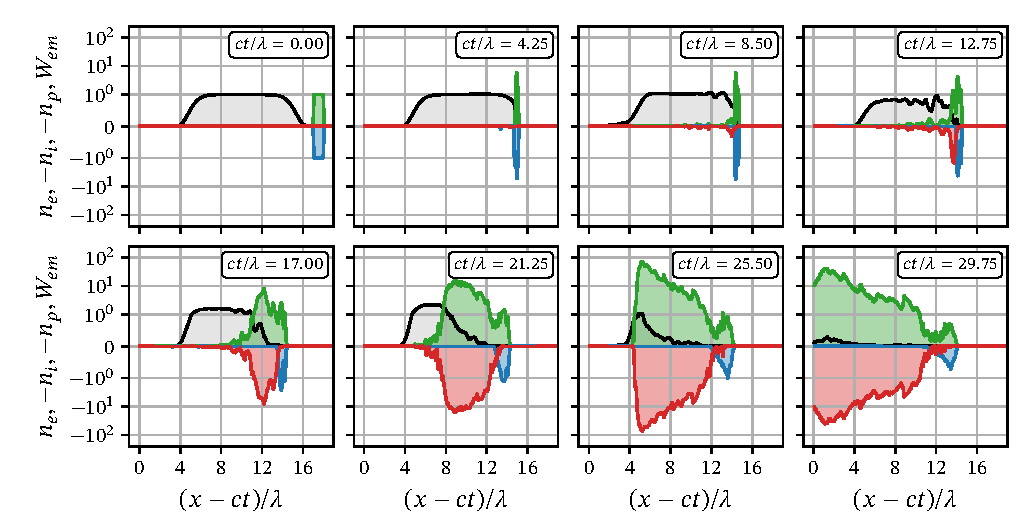
\includegraphics{cushion-onaxis.pdf}}
	\caption[Распределение плотности частиц и электромагнитной энергии в различные моменты времени в численном моделировании]{\label{Sim_res} Распределение плотности частиц (зелёная линия~---~электроны, синяя~---~ионы, красная~---~позитроны) и электромагнитной энергии (чёрная линия) вдоль оси $x$ в различные моменты времени. Значения нормированы на максимальные начальные значения. Масштаб вертикальной оси линейный для значений $[-1,1]$ и логарифмический для остальных значений.}
\end{figure}

\begin{figure}[h!]
	\centerfloat{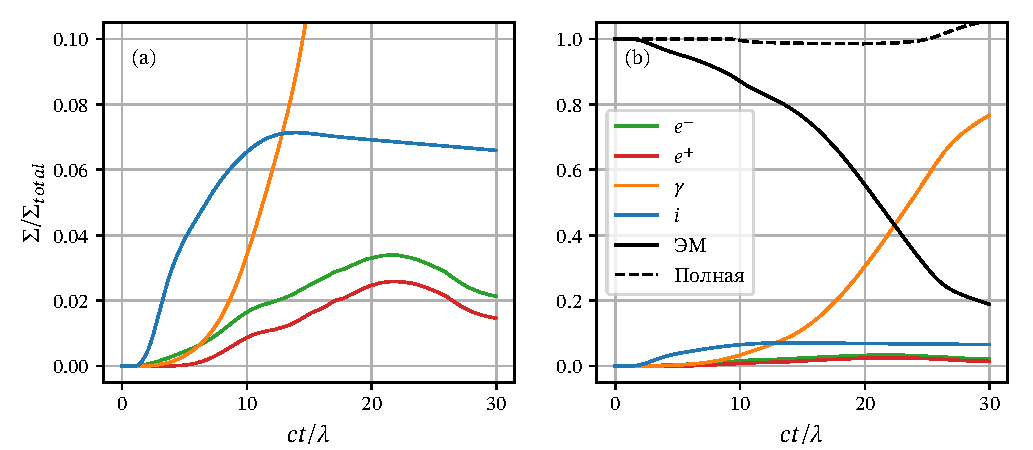
\includegraphics{cushion-energy.pdf} }
	\caption[Баланс энергии в системе в численном моделировании с параметрами $n_{e}=\SI{5.9e23}{\centi\meter^{-3}}$, $d=1$~мкм, $a_{0}=2500$]{\label{Sim_en} (a) Часть энергии лазерного импульса, перешедшая в энергию частиц, как функция времени. (b) Полная энергия системы, энергия лазерного импульса и энергия гамма-квантов, нормированные на начальное значение полной энергии.}
\end{figure}

Временная эволюция плотности частиц и электромагнитной энергии представлена на Рис.~\ref{Sim_res} для счёта с параметрами: ${n_{e}=\SI{5.9e23}{\centi\meter^{-3}}\approx530\, n_\mathrm{cr}}$ (${n_\mathrm{cr}=m_{e}\omega_{L}^{2}/4\pi e^{2}\approx\SI{1e21}{\centi\meter^{-3}}}$~---~критическая концентрация), $d=1$~мкм, $a_{0}=2500$. 
Из анализа результатов численного моделирования следует, что до времени $ct/\lambda\lesssim 8$ мишень сжимается в тонкий слой и ускоряется в продольном направлении до скорости, близкой к скорости света, т.е. происходит типичное ускорение ионов в режиме <<светового паруса>> (см. Рис.~\ref{Sim_en}\;(a)). 
Число электрон-позитронных пар, образованных в течение этого времени, незначительно. В интервал времени $8~\lesssim~ct/\lambda~\lesssim~14$ начинает формироваться неоднородная электрон-позитронная плазма, которая частично поглощает излучение, что приводит к снижению эффективности ускорения ионов (см. Рис.~\ref{Sim_en}\;(a)).
В период времени $14~\lesssim~ct/\lambda~\lesssim~28$ КЭД каскад развивается в самоподдерживающемся режиме, т.е. без участия частиц начальной затравки. 
При этом передний (по отношению к лазерному импульсу) фронт распределения электрон-позитронной пары движется со скоростью $v_\mathrm{fr}$ меньшей, чем скорость света; задний фронт при этом по инерции движется вместе с мишенью практически со световой скоростью. 
Таким образом электрон-позитронная подушка расширяется навстречу лазерному излучению и в конце концов полностью поглощает его. 
Такое поведение во многом напоминает распространение фронта ионизации при СВЧ пробое в газе \cite{semenov1982breakdown}.

\begin{figure}[h!]
	% \includegraphics[width=1\linewidth]{x_t2.pdf}
    \centerfloat{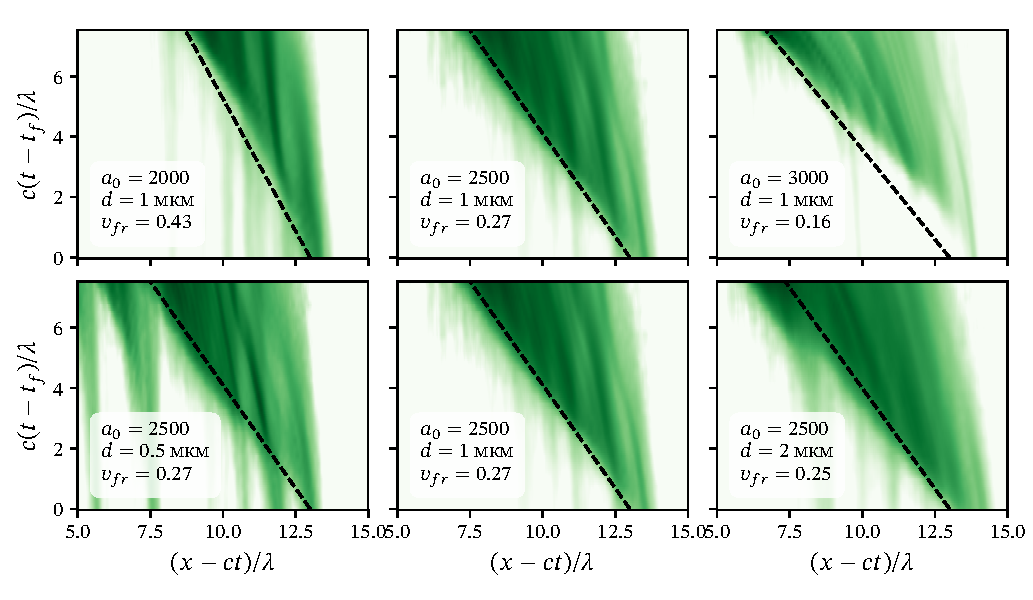
\includegraphics{cushion-xt.pdf}}
    \caption[Распределение позитронов в плоскости $x-t$ в численных моделированиях с различными начальными параметрами]{
        \label{fig:ch2/cushion-x-t}
        Распределение позитронов в плоскости $x-t$. Более яркий цвет обозначает большую плотность. Значения скорости фронта каскада (белые штриховые линии) даны в лабораторной системе отсчёта. $t_{f}$~---~приблизительное время начала образования подушки. $ct_{f}/\lambda\approx17.5$ для $a_{0}=2000$, $ct_{f}/\lambda\approx15.0$ для $a_{0}=2500$, $ct_{f}/\lambda\approx12.5$ для $a_{0}=3000$.}
\end{figure}

Мы провели ряд численных счётов с различными значениями $a_{0}=1500$, $2000$, $2500$, $3000$ и мишенью толщиной $d=1$~мкм и с различными значениями $d=0.5$~мкм, $1$~мкм, $2$~мкм для $a_{0}=2500$. 
На Рис.~\ref{fig:ch2/cushion-x-t} видно, что скорость фронта каскада слабо зависит от времени и толщины мишени, тогда как сильно зависит от интенсивности лазерного импульса, уменьшаясь (в лабораторной системе отсчёта) с её ростом. 
Также стоит отметить, что на поздних стадиях взаимодействия концентрация электрон-позитронной плазмы в несколько раз превышает значение релятивистской критической концентрации~$a_0 n_\mathrm{cr}$. 
Во всех проведённых счётах каскад эффективно развивается, однако, при $a_0=1500$ концентрация плазмы достигает значения $0.6 a_0 n_\mathrm{cr}$ к концу моделирования ($t = 30 \lambda/c$).
Поэтому мы предполагаем, что значение $a_0=1500$ грубо является пороговым значением для развития самоподдерживающегося каскада в плоской волне.

Для того, чтобы определить роль ионов мишени в образовании КЭД каскада, мы провели моделирование взаимодействия лазерного импульса с закритической электрон-позитронной мишенью. 
Геометрия мишени и импульса выбрана такой же, как описано выше. 
Толщина мишени составляла $d=1$~мкм, концентрация электронов $n_e = 0.7 a_0 n_\mathrm{cr}$, $a_0=2500$. 
Анализ результатов моделирования показывает, что самоподдерживающийся КЭД каскад развивается таким же образом, как и при затравке из электрон-ионной мишени; более того, совпадает и скорость фронта каскада. 
Из этого можно сделать вывод, что определённым выбором затравки и достаточно высокой интенсивностью лазерного импульса можно добиться развития КЭД каскада А-типа в поле с конфигурацией, близкой к плоской волне.

\begin{figure}[h!]
	\center{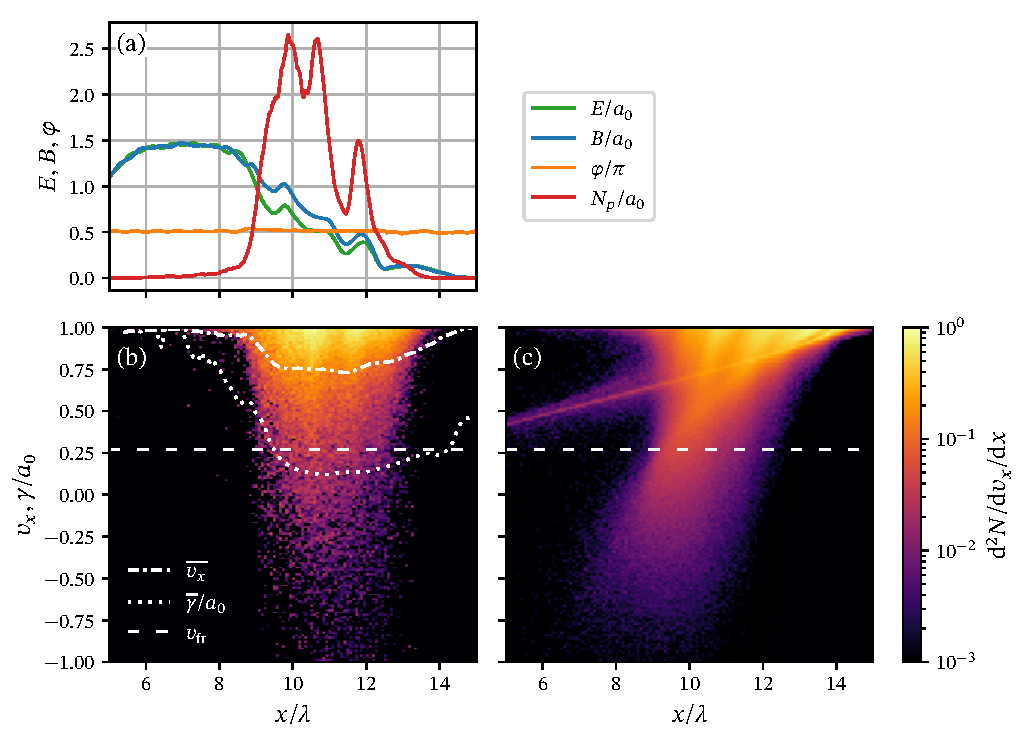
\includegraphics{cushion-fields-particles.pdf}}
    \caption[Результаты численного моделирования развития КЭД каскада в плоской волн]{\label{fig:ch2/field-structure} Результаты численного моделирования в момент времени ${t = 20 \lambda / c}$. (а) Распределение амплитуды электрического поля $E$, амплитуды магнитного поля $B$, угла $\varphi$ между ними и концентрации позитронов $N_p$. Распределение (b) позитронов ((с) гамма-квантов) в плоскости $x - v_{x}$ (плотность частиц обозначена цветом), их средние продольная скорость $\overline{v_x}$ (белая штрих-пунктирная линия) и Лоренц-фактор $\overline{\gamma}$ (белая пунктирная линия) как функции $x$. Белой штриховой линией обозначена скорость фронта каскада $v_\mathrm{fr}$ (равная 0.27 в данном моделировании).}
\end{figure}

\begin{figure}[h!]
	\center{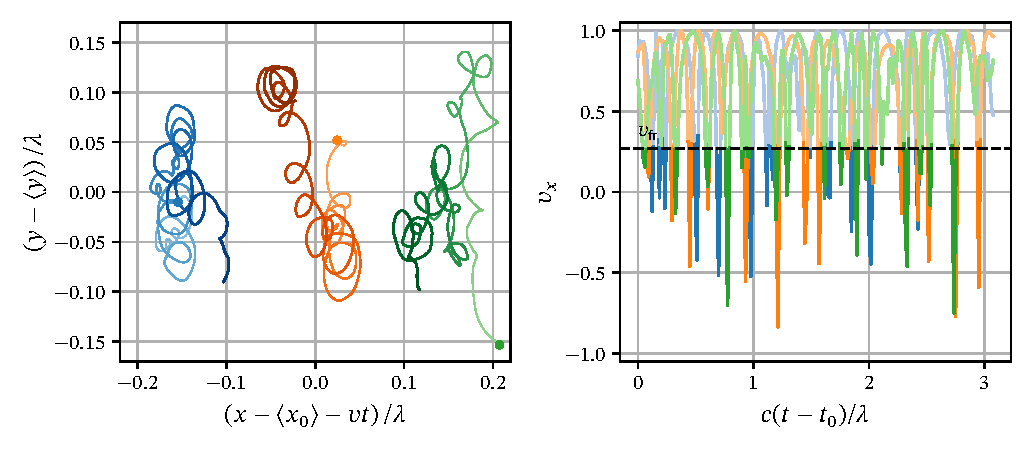
\includegraphics{cushion-tracks.pdf}}
    \caption[Характеристики движения отдельных электронов, находящихся внутри электрон-позитронной подушки.]{\label{fig:ch2/sec1/tracks} Характеристики движения трёх электронов, находящихся внутри электрон-позитронной подушки. (a) Траектории электронов в плоскости $xy$, в системе отсчёта, движущейся со скоростью $v=0.7$. Положение частицы в более поздние моменты времени обозначено более тёмным цветом, начальное положение частицы отмечено кружком. (b) Зависимость продольной скорости в зависимости от времени. Чёрная пунктирная линия соответствует скорости фронта каскада $v_\mathrm{fr} = 0.27$.}
\end{figure}

\subsection{Ключевые особенности и механизм развития КЭД каскада}
\label{sub:ch2/sec2/Mechanism}

Рассмотрим более подробно распределение электромагнитного поля и динамику частиц внутри электрон-позитронной плазмы для определения механизма развития каскада. 
Из Рис.~\ref{fig:ch2/field-structure}~(a) следует, что структура поля близка к циркулярно-поляризованной волне с перпендикулярными электрической и магнитной компонентами, $\vb{E \perp B}$, и поле затухает в плазме на масштабе в несколько длин волн. 
Ключевая особенность конфигурации поля~---~преобладание магнитного поля над электрическим, $B > E$.
В таком поле электроны и позитроны не набирают энергию (см. линию $\overline{\gamma} / a_0$ на  Рис.~\ref{fig:ch2/field-structure}~(b)), поэтому развитие каскада внутри плазмы подавлено.
Более того в таком поле траектории частиц представляют собой винтовые линии (см. Рис.~\ref{fig:ch2/sec1/tracks}~(a)). 
Это легко объясняется, если мы перейдём в систему отсчёта, движущуюся со скоростью $[\vb{E}~\times~\vb{B}]_x / B^2$, в которой электрическое поле параллельно магнитному и меньше его. 
В таком поле частицы вращаются в плоскости, перпендикулярной магнитному полю и могут иметь компоненту скорости вдоль магнитного поля. 
В лабораторной системе электроны и позитроны в среднем обгоняют фронт каскада, однако, из-за вращения частиц их мгновенная скорость вдоль оси $x$ иногда может быть меньше скорости фронта (см.  Рис.~\ref{fig:ch2/field-structure}~(b) и Рис.~\ref{fig:ch2/sec1/tracks}~(b)). 
В такие моменты частицы могут излучить гамма-квант, который попадёт в вакуумную область (большое количество гамма-квантов, распространяющихся медленнее фронта каскада и даже навстречу лазерному излучения, наблюдается в численном моделировании, что продемонстрировано на Рис.~\ref{fig:ch2/field-structure} (c)) и родит в сильном поле новую пару. 
Эта пара ускоряется сильным поле внутрь плазмы, где магнитное поле больше электрического и процесс повторяется.
Таким образом, самоподдерживающееся развитие каскада происходит на границе вакуума и подушки.
Важно подчеркнуть принципиальное различие между \textit{вакуумной} и \textit{плазменной} областями: в первой электромагнитная энергия передается каскадным частицам, а во второй частицы не ускоряются, а высвобождают полученную энергию в виде гамма-излучения.
Некоторая часть этого излучения возвращается обратно в область вакуума и обеспечивает положительную обратную связь, необходимую для поддержания каскада.
Механизм поддержания КЭД каскада в плоской волне схематически представлен на рисунке~\ref{fig:ch2/sec2/scheme}.

% \begin{figure}[h!]
% 	\center{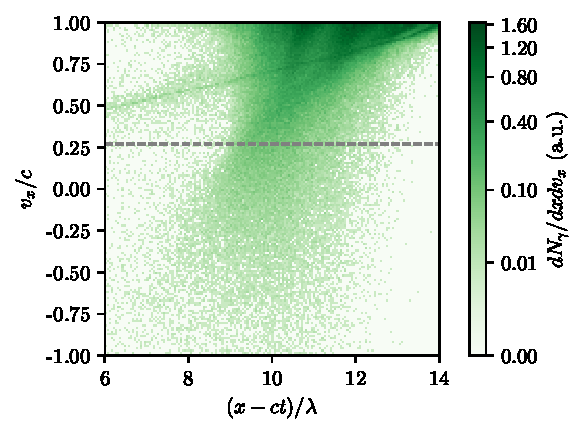
\includegraphics[width=100mm]{gamma2.pdf}}
% 	\caption{\label{gamma10} \fixme{Распределение гамма-квантов в плоскости $x - v_x$ в момент времени $t=20 \lambda /c $. Серая пунктирная линия обозначает скорость фронта $v_\mathrm{fr}$.} }
% \end{figure}


\begin{figure}[ht]
    \centerfloat{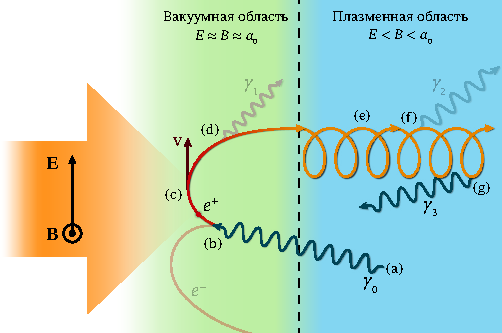
\includegraphics[width=155mm]{cushion-scheme.pdf}}
    \caption[Механизм поддержания КЭД каскада в плоской волне]{
    Схематическое изображение механизма поддержания КЭД каскада. (a), (f), (g) Излучение \textit{активного} (см. ниже) гамма-кванта в плазменной области, (b) распад \textit{активного} гамма-кванта в вакуумной области, (c) ускорение электрона и позитрона в плоской волне, (d) излучение \textit{пассивного} гамма-кванта в вакуумной области, (e) движение позитрона по винтовой линии в плазменной области.}
    \label{fig:ch2/sec2/scheme}
\end{figure}

\section{Аналитическое описание самоподдерживающегося КЭД каскада в плоской волне}
\label{sec:ch2/sec3}

Приступим к аналитическому описанию описанных выше процессов.
Аналогично работам~\cite{nerush2011analytical, elkina2011qed} запишем кинетические уравнения для электронов, позитронов и гамма-квантов, предполагая, что КЭД каскад находится на стадии самоподдержания, поэтому затравочные частицы, например, электроны и ионы начальной мишени, не влияют на его развитие.
Кинетические уравнения совместно с уравнениями Максвелла (в виде теоремы Пойнтинга) записываются в следующем виде
\begin{align}
    \label{eq:ch2/Boltzman1}
    \pdv{f_{e^\pm}}{t} +  \vb{v}_{e^\pm} \nabla f_{e^\pm} \pm \left( \vb{E} + [\vb{v}_{e^\pm} \times \vb{B}] \right) \pdv{ f_{e^\pm}}{ \vb{p}} \ &
    \begin{aligned}[t]
        = & \int f_\gamma(\vb{p'}) w_\mathrm{pair}(\vb{p', p}) \dd\vb{p'} + \\
        + & \int f_{e^\pm}(\vb{p'}) w_\mathrm{rad}(\vb{p', p}) \dd\vb{p'} - \\
        - & \int f_{e^\pm}(\vb{p}) w_\mathrm{rad}(\vb{p, p'}) \dd\vb{p'}  ,
    \end{aligned} \\
    \label{eq:ch2/Boltzman2}
    \pdv{f_\gamma}{t} + \vb{v}_\gamma\nabla f_\gamma \ &
    \begin{aligned}[t]
        = &\int  f_{e^\pm}(\vb{p'}) w_\mathrm{rad}(\vb{p', p'-p}) \dd\vb{p'} - \\ 
        + &\int f_\gamma(\vb{p}) w_\mathrm{pair}(\vb{p, p'}) \dd\vb{p'} ,
    \end{aligned} \\
    \label{eq:ch2/Max1}
    \pdv{}{t}\left( \frac{E^2 + B^2}{2} \right) + \nabla [\vb{E}\times\vb{B}] &= \int f_{e^-}(\vb{p}) (\vb{v}_{e^-} \vb{E}) \dd\vb{p} - \\
    &- \int f_{e^+}(\vb{p}) (\vb{v}_{e^+}\vb{E}) \dd\vb{p} ,
    % \frac{\partial \vb{B}}{\partial t} + \nabla\times \vb{E} &= 0, \\
    % \label{eq:ch2/Max2}
    % \frac{\partial \vb{E}}{\partial t} - \nabla\times \vb{B} &=  \int f_{e^-} \vb{v}_{e^-} \dd\vb{p} -  \int f_{e^+} \vb{v}_{e^+} d\vb{p} ,
\end{align}
где $f_{e^\pm,\gamma}(t,\vb{r,p})$~---~функции распределения электронов, позитронов и гамма-квантов соответственно, $\vb{v}$~---~скорость частиц, равная $\vb{p}/\sqrt{1+p^2}$ для электронов и позитронов и равная $\vb{p}/p$ для гамма-квантов, $w_\mathrm{rad}(\vb{p', p})\dd\vb{p'}$~---~вероятность излучения электроном или позитроном с импульсом $\vb{p'}$ гамма-кванта с импульсом $\vb{p'-p}$ в единицу времени, $w_\mathrm{pair}(\vb{p', p})\dd\vb{p'}$~---~вероятность распада гамма-кванта с импульсом $\vb{p'}$ на электрон с импульсом $\vb{p}$ и позитрон с импульсом $\vb{p'-p}$ в единицу времени.
Здесь также используется уже описанная выше релятивистская нормировка, при которой электрическое и магнитное поля нормируются на величину $m_ec\omega_\mathrm{L}/e$, концентрация частиц~---~на критическую концентрацию $n_\mathrm{cr}=m_e\omega_\mathrm{L}^2/4\pi e^2$, энергия и импульс~---~на $m_e c^2$ и $m_e c$ соответственно, координаты и время~---~на $c/\omega_\mathrm{L}$ и $1/\omega_\mathrm{L}$ соответственно.

\subsection{Предположения модели}
\label{sub:ch2/sec3/Assumptions}
Применим ряд упрощений к записанным выше уравнениям.
Во-первых, т.к. исследуется взаимодействие с плоской ЭМ волной, то будем считать задачу пространственно одномерной.
Более того, будем рассматривать взаимодействие с циркулярно-поляризованной волн, что приводит к симметрии относительно поворота вдоль оси распространения волны (для определённости оси $x$ здесь и далее).
Данные предположения приводят к тому, что функции распределения частиц становятся зависимыми только от трёх переменных (исключая время) вместо шести, т.е. $f(t;\vb{r},\vb{p})=f(t;x,p,\theta)/2\pi$, где $p$~---~импульс частицы, $\theta$~---~угол между вектором импульса частицы и осью симметрии $x$.

Во-вторых, предположим, что функции распределения являются локально моноэнергитическими, т.е. $f\propto\delta(p-\overline{p}(x))/p^2$, где $\overline{p}(x)$~---~среднее значение импульса частиц, расположенных в малой окрестности $x$.
Обозначим среднюю энергию гамма-квантов как $\varepsilon_\gamma$, и среднюю энергию электрон-позитронных пар как $\varepsilon_p$, предполагая, что они ультрарелятивистские, поэтому $\varepsilon_p^2 = 1+p_p^2\approx p_p^2$.
Несмотря на то, что моноэнергитическое приближение является сильно упрощающим, мы предполагаем, что механизм развития и КЭД каскада, описанный выше, принципиально не зависит от каких-либо особенностей спектра частиц.
Поэтому мы утверждаем, что учет эволюции энергетических спектров в нашей модели вызовет только количественные, а не качественные изменения, при этом сильно усложняя уравнения.
Как будет показано ниже, это предположение справедливо для пар, которые попадают в область плотной электрон-позитронной плазмы с примерно равными энергиями.
Для гамма-квантов мы используем двухпотоковое приближение, т.е. разделяем гамма-кванты на те, которые излучаются в вакуумной области и распространяются в основном вдоль направления распространения лазерного импульса и, таким образом, не дают вклада в развитие каскада (мы обозначим их как \textit{пассивные} гамма-кванты) и те, которые излучаются в области плазмы в различных направлениях и обеспечивают положительную обратную связь, необходимую для развития каскада (мы обозначаем их либо как \textit{активные} гамма-кванты, либо просто гамма-кванты).
Как видно из Рис.~\ref{fig:ch2/sec3/gamma_energy} энергетический спектр гамма-квантов является достаточно широким, однако если исключить пассивные гамма-кванты, то ширина спектра значительно уменьшается, что оправдывает наше предположение.
Поскольку пассивные гамма-кванты влияют на развитие каскада только забирая часть общей энергии, их пространственное распределение не имеет значения для развития каскада, однако оно всё равно будет рассчитано для более точного сравнения с результатами QED-PIC моделирования.

\begin{figure}[ht]
    \centerfloat{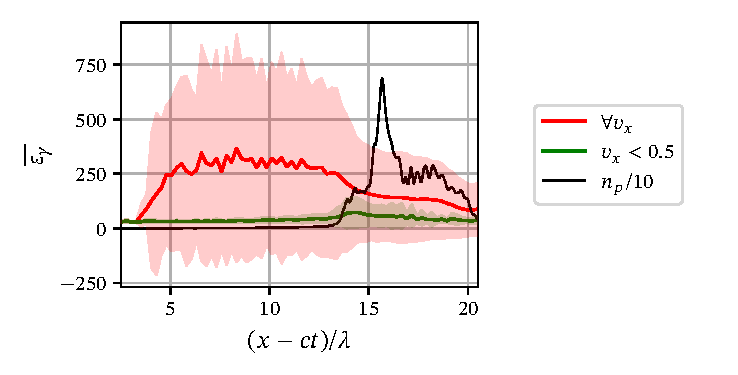
\includegraphics{cushion-gamma-energy}}
    \caption[Сравнение ширины разброса энергий всех гамма-квантов и только активных гамма-квантов]{\label{fig:ch2/sec3/gamma_energy} 
    Средняя энергия $\varepsilon_\gamma$ гамма-квантов в зависимости от координаты $x$, рассчитанная по всем частицам (красная линия) и только по частицам со скоростью вдоль оси  $x$ не превышающей 0.5, что по нашим предположениям включает только активные гамма-кванты (зелёная линия). Закрашенные цветные области отображают среднеквадратичное отклонение энергии. Данные взяты из результатов PIC моделирования в момента времени $ct/\lambda=18$. Параметры моделирования обсуждаются в подразделе~\ref{sub:ch2/sec3/Numeric}. Начальные условия такие же, как на Рис.~\ref{fig:ch2/sec3/sol2500}. Чёрная линия соответствует распределению плотности электрон-позитронной плазмы.}
\end{figure}

Для того, чтобы опустить интегрирование по энергиям и азимутальному углу $\varphi$ (в плоскости $yz$), переопределим функции распределения $f$ следующим образом
\begin{equation}
    f(x, \varepsilon, \theta, \varphi) \rightarrow \int\limits_0^\infty\int\limits_0^{2\pi}f(x,\varepsilon,\theta,\varphi)2\pi\varepsilon^2\dd\varphi \dd\varepsilon = n(x)\Phi(\theta),
\end{equation}
где $n(x)$~---~концентрация частиц, $\Phi(\theta)$~---~функция распределения импульса частиц по углу $\theta$, причём
\begin{align}
    \int\limits_{-\infty}^{+\infty} n(x)\dd x = N, \\
    \int\limits_0^\pi \Phi(\theta)\sin\theta \dd\theta = 1,
\end{align}
где $N$~---~полное число частиц.

Предположение о моноэнергитичности фактически соответствует переходу от кинетического к гидродинамическому описанию, т.е. записи уравнений на моменты функций распределения.
Чтобы записать гидродинамические уравнения предварительно введём несколько дополнительных величин
\begin{align}
    \label{eq:ch2/Wpair0}
    W_\mathrm{pair}(\chi_\gamma, \varepsilon_\gamma) = \int w_\mathrm{pair}(\vb{p},\vb{p'})\dd\vb{p'} ,\\
    \label{eq:ch2/Wrad0}
    W_\mathrm{rad}(\chi_p, \varepsilon_p) = \int w_\mathrm{rad}(\vb{p},\vb{p'})\dd\vb{p'} ,\\
    \label{eq:ch2/Irad0}
    I_\mathrm{rad}(\chi_p) = \int w_\mathrm{rad}(\vb{p},\vb{p'})(\varepsilon_p-\varepsilon_p')\dd\vb{p'},
\end{align}
где $W_\mathrm{pair}, W_\mathrm{rad}, I_\mathrm{rad}$~---~полная вероятность фотообразования электрон-позитронных пар, полная вероятность и мощность излучения гамма-квантов соответственно~\cite{Baier98}. 
Как неоднократно указывалось выше, данные величины зависят от Лоренц-инвариантного КЭД параметра $\chi$
\begin{equation}
    \chi = \frac{\varepsilon}{a_\mathrm{S}} \sqrt{ \left(\vb{E}+\vb{v}\times\vb{B}\right)^{2}-\left(\vb{v}\cdot\vb{E}\right)^{2} } ,
\end{equation}
где $\varepsilon$~---~энергия частицы, $a_\mathrm{S} = e E_\mathrm{S}/m_ec\omega_\mathrm{L} = m_ec^2/\hbar\omega_\mathrm{L}$ и $a_\mathrm{S}={m_e}^2c^3/\hbar e$~---~поле Заутера-Швингера~\cite{berestetskii1982quantum}.
В общем виде гидродинамические уравнения выглядят как уравнения переноса (непрерывности)
\begin{equation}
    \pdv{ D_\alpha}{ t} + \pdv{ F_\alpha}{ x} = \sum_{\beta} S[\alpha, \beta] ,
\end{equation}
где $D_\alpha$ и $F_\alpha$~---~плотность и поток некоторой физической величины $\alpha$, $S[\alpha,\beta]$~---~источник, приводящий к изменению величины $\alpha$ в результате процесса $\beta$.
Отметим, что несмотря на то, что мы определили функцию распределения частиц по энергиям, для вычисления источников $S[\alpha,\beta]$ также необходимо знать угловое распределение частиц, которое обсуждается ниже.
Основываясь на качественном объяснении механизма развития и поддержания КЭД каскада, описанном в подразделе~\ref{sub:ch2/sec2/Mechanism}, мы предполагаем, что следующая система уравнений достаточно полно описывает данный процесс 
\begin{align}
    \label{eq:ch2/hd_p1}
    \frac{\partial }{\partial t}n_p  \quad &\!+\!& &\frac{\partial}{\partial x}\left( v_x n_p \right) \!\!\!&\!&\!=  S[n, \mathrm{pp}] ,\\
    \label{eq:ch2/hd_p2}
    \frac{\partial}{\partial t}\left( \varepsilon_p n_p \right)   \quad &\!+\!& & \frac{\partial}{\partial x}\left( v_x \varepsilon_p n_p \right) \!\!\!&\!&\!=
    \begin{aligned}[t]
        & S[\varepsilon, \mathrm{pp}] + S[\varepsilon, \mathrm{\mathrm{acc}}] \psi_\mathrm{vac} - \\
        & - S[\varepsilon, \mathrm{rad_a}] \psi_\mathrm{pl} - S[\varepsilon, \mathrm{rad_p}] \psi_\mathrm{vac} ,
    \end{aligned} \\
    \label{eq:ch2/hd_g1}
    \frac{\partial }{\partial t}n_\gamma  \quad &\!+\!& &\frac{\partial}{\partial x}\left( \overline{v_{\gamma\parallel}} n_\gamma \right)\!\!\!&\!&\!= -S[n, \mathrm{pp}] + 2 S[n, \mathrm{rad_a}] \psi_\mathrm{pl} ,\\
    \label{eq:ch2/hd_g2}
    \frac{\partial}{\partial t}\left( \overline{v_{\gamma\parallel}} n_\gamma \right) \quad &\!+\!& & \frac{\partial}{\partial x}\left( \overline{v_{\gamma\parallel}^2} n_\gamma \right) \!\!\!&\!&\!=  -S[v, \mathrm{pp}] + 2 S[v, \mathrm{rad_a}] \psi_\mathrm{pl} ,\\
    \label{eq:ch2/hd_g3}
    \frac{\partial}{\partial t}\left( \varepsilon_\gamma n_\gamma \right) \quad &\!+\!& &\frac{\partial}{\partial x}\left( \overline{v_{\gamma\parallel}} \varepsilon_\gamma n_\gamma \right) \!\!\!&\!&\!= -S[\varepsilon, \mathrm{pp}] + 2 S[\varepsilon, \mathrm{rad_a}] \psi_\mathrm{pl} ,\\
    \label{eq:ch2/hd_e1}
    \frac{\partial }{\partial t}\left( \frac{E^2 + B^2}{2} \right) \quad &\!+\!& &\frac{\partial}{\partial x} {\left[ \vb{E\times B} \right]}_x \!\!\!&\!&\!= - 2 S[\varepsilon, \mathrm{\mathrm{acc}}]\psi_\mathrm{vac} \equiv - \vb{jE} ,\\
    && & \qquad\quad \frac{\partial \Sigma_\gamma}{\partial t} \!\!\!&\!&\!= 2 \int\limits_0^\infty S[\varepsilon, \mathrm{rad_p}]\psi_\mathrm{vac} dx ,
\end{align}
где $n_p = n_{e^+} = n_{e^-}$~---~половина концентрации электрон-позитронной плазмы в предположении её квазинейтральности, $v_x$~---~средняя продольная скорость пар, рассчитываемая в подразделе~\ref{sub:ch2/sec3/fields}, $\overline{v_{\gamma\parallel}}$ и $\overline{v_{\gamma\parallel}^2}$~---~средняя величина и средний квадрат величины продольной скорости гамма-квантов.
Последние рассчитываются из углового распределения следующим образом
\begin{align}
    \overline{v_{\gamma\parallel}} = \int_0^\pi \Phi(\theta)\cos\theta\sin\theta d\theta, \\
    \overline{v_{\gamma\parallel}^2} = \int_0^\pi \Phi(\theta)\cos^2\theta\sin\theta d\theta.
\end{align}
Уравнение~\eqref{eq:ch2/hd_e1} является записью теоремы Пойнтинга, и которое фактически является уравнением переноса плотности электромагнитной энергии.
Источники $S[n,\beta]$, $S[v,\beta]$ и $S[\varepsilon,\beta]$ соответствуют изменению концентрации, продольной скорости и энергии частиц соответственно, источники $S[\alpha, \mathrm{pp}]$, $S[\alpha, \mathrm{acc}]$, $S[\alpha, \mathrm{rad_a}]$ и $S[\alpha, \mathrm{rad_p}]$ соответствуют процессам фотообразования пар, ускорения пар в плоской волне, излучению активных гамма-квантов парами в плазменной области и излучению пассивных гамма-квантов парами в вакуумной области соответственно (отмечены соответственно буквами (b), (c), (d) и (f) на Рис.~\ref{fig:ch2/sec2/scheme}), $\Sigma_\gamma$~---~полная энергия пассивных гамма-квантов.
Множитель $\psi_\mathrm{vac}(\psi_\mathrm{pl})$ считается равным 1 в вакуумной (плазменной) области и 0 в плазменной (вакуумной) области.
Вычисление данных множителей будет приведено ниже.
Отметим, что $\psi_\mathrm{vac}+\psi_\mathrm{pl}=1$.
Для удобства будем опускать дынные множители, когда рассматриваемая область очевидна.

\subsection{Конфигурация электромагнитного поля}
\label{sub:ch2/sec3/fields}

Согласно результатом трёхмерного QED-PIC моделирования электрическое и магнитное поля в плазменной области остаются практически перпендикулярными друг другу, а величина магнитного поля всюду превосходит величину электрического: $B > E$.
Пространственное распределение ЭМ поля имеет характерный масштаб $\lambda$ как в вакуумной, так и в плазменной области.
В таком поле заряженные частицы дрейфуют в направлении перпендикулярном, как электрическому, так и магнитному полю, т.е. вдоль оси $x$ со скоростью
\begin{equation}
    \label{eq:ch2/vdrift}
    v_x\approx E/B.
\end{equation}
В вакуумной области ЭМ поле представляет собой поле падающей плоской волны.
В таком случае электрическое и магнитное поля взаимно перпендикулярны и равны друг другу по величине.
Если энергия $\varepsilon$ частицы, попавшей в вакуумную область, меньше безразмерной амплитуды поля $E$, то согласно построенной в первой главе асимптотической теории за время, много меньшее периода волны, такая частица ускорится в продольном направлении практически до скорости света.
Таким образом можно считать, что в вакуумной области выполняется соотношение $v_x\approx 1=E/B$, т.е. уравнение~\eqref{eq:ch2/vdrift} в действительности справедливо как в плазменной, так и в вакуумной области.

В данном рассуждении мы не учитываем отражённую от границы $e^-e^+$ плазмы волну по нескольким причинам.
Во-первых, в трёхмерном QED-PIC моделировании не наблюдается существенного отражения при развитии каскада на стадии его самоподдержания.
Во-вторых, отражение, возникающее на начальном этапе лазерного взаимодействия с тонкой твердой мишенью, согласно теории относительности, быстро истощается по мере ускорения частиц в направлении распространения лазерного импульса и, таким образом, становится несущественным для более поздних стадий развития каскада.
Однако наша модель не описывает электрон-ионную плазму, поэтому мы исследуем взаимодействие лазерного импульса с затравкой в виде встречного гамма-сгустка (см. подраздел~\ref{sub:ch2/sec3/Numeric}), где отражения не происходит даже на начальном этапе взаимодействия.
Кроме того, отражение незначительно изменило бы процесс фоторождения пар в связи с тем, что наибольшей вероятностью распада обладают гамма-кванты, распространяющиеся навстречу лазерному импульсу, т.е. попутно отраженному излучению.
А поля попутной волны не увеличивают значение определяющего КЭД-параметра $\chi$ гамма-квантов.
Наконец, в вакуумной области, где лазерное поле наиболее сильное, находятся в основном ультрарелятивистские электроны и позитроны, образованные из фотонов с наиболее высокой энергией.
Рассеяние релятивистски сильного лазерного поля ($a_0 \gg 1$) на ультрарелятивистских электронах и позитронах ($\gamma \gg 1$) происходит как в нелинейном, так и в квантовом режиме.
Из-за этого, а также из-за того, что положение частиц нескоррелировано, результирующее рассеянное излучение некогерентно и его частота сильно сдвинута вверх.
Такое излучение лучше всего описывается отдельными фотонами, как это и реализовано в коде QUILL.
Часть этих фотонов, распространяющихся навстречу лазерному импульсу, действительно можно рассматривать как отражение.
Хотя такие фотоны могут увеличить общий выход электрон-позитронных пар и гамма-квантов за счет КЭД процессов более высокого порядка, они значительно менее вероятны, чем нелинейное комптоновское рассеяние и процесс Брейта-Уилера, и поэтому не учитываются ни в QED-PIC моделировании, ни в нашей модели.
Отметим, однако, что в нашей модели учитываются потери энергии из-за некогерентного гамма-излучения как в вакуумной, так и в плазменной областях.

\subsection{Функция распределения активных гамма-квантов}
\label{sub:ch2/sec3/gammas}

Как описано в разделе~\ref{sub:ch2/sec2/Mechanism} активные гамма-кванты излучаются парами в процессе их движения по винтовым траекториям в плазменной области.
В связи с этим их угловое распределение является широким.
Предположим также, что это распределение плавное и может быть описано всего одним параметром.
Данным параметром является скорость $v$ мгновенной системы отсчёта $K'$, в которой угловое распределение фотонов, находящихся вблизи малой окрестности координаты $x$, является практически изотропным, т.е.
\begin{equation}
    \Phi'(\theta') \equiv \frac{\dd N'}{\dd \cos\theta'} = \frac{1}{2},
\end{equation}
где $\dd N'=\dd N$~---~число частиц с продольной скоростью в диапазоне $[\cos\theta', \cos\theta'+\dd\cos\theta']$ и
\begin{equation}
    \cos\theta' = \frac{\cos\theta - v}{1 - v \cos\theta}.
\end{equation}
В лабораторной системе отсчёта такое распределение выглядит следующим образом~\cite{LandauII}
\begin{equation}
    \label{eq:ch2/Phi}
    \Phi(\theta, v) = \frac{\dd N}{\dd \cos\theta} = \frac{\dd N'}{\dd \cos\theta'} \frac{\dd \cos\theta'}{\dd \cos\theta} = \frac{1-v^2}{{2\left( 1 - v \cos{\theta}  \right)}^2}.
\end{equation}
Таким образом, функция распределения активных гамма-квантов имеет следующий вид
\begin{equation}
    f_\gamma(t; x,\theta)=\Phi\left(\theta, v_{\gamma\parallel}(x,t)\right) n_\gamma(x,t).
\end{equation}
Средняя величина $\overline{v_{\gamma\parallel}}$ и средний квадрат величины $\overline{v_{\gamma\parallel}^2}$ продольной скорости рассчитываются следующим образом
\begin{align}
    \label{eq:ch2/av_vx}
    \overline{v_{\gamma\parallel}}=\int_0^\pi \Phi(\theta, v) \cos{\theta} \sin{\theta}\dd\theta = \frac{1}{v_{\gamma\parallel}} - \frac{1-v_{\gamma\parallel}^2}{v_{\gamma\parallel}^2}\text{ath}(v_{\gamma\parallel}) , \\
    \overline{v_{\gamma\parallel}^2}=\int_0^\pi \Phi(\theta, v) \cos^2{\theta} \sin{\theta}\dd\theta = \frac{2\overline{v_{\gamma\parallel}}}{v_{\gamma\parallel}} - 1 ,
\end{align}
где $\text{ath}(x)$~---~обратная функция гиперболического тангенса.
Отметим, что согласно преобразованиям Лоренца средняя скорость гамма-квантов $\overline{v_{\gamma\parallel}}$ отличается от скорости $v_{\gamma\parallel}$ системы отсчёта $K'$, в которой их распределение изотропно.
Результаты QED-PIC моделирования показывают, что выражение~\eqref{eq:ch2/Phi} является достаточно хорошей аппроксимацией углового распределения активных гамма-квантов (см. Рис.~\ref{fig:ch2/sec3/ang} (a), (b)).

\begin{figure}[ht]
    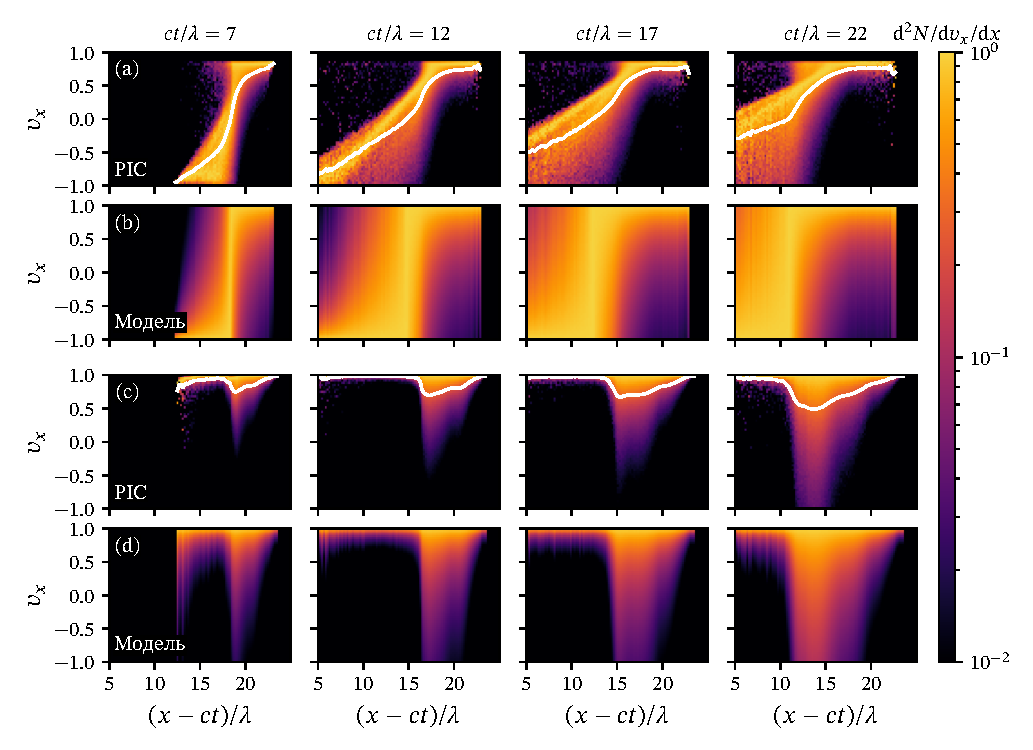
\includegraphics{cushion-ang-new.pdf}
    \caption[Проверка приближения, использованного для описания углового распределения частиц.]{\label{fig:ch2/sec3/ang}
    Проверка приближения, использованного для описания углового распределения частиц. Угловое распределение частиц ((a)~---~гамма-квантов, (c)~---~$e^-e^+$ пар), расположенных в малой окрестности координаты $x$ (цветовая карта) и их средняя продольная скорость, рассчитанная по этому распределению (белая линия) согласно результатам численного QED-PIC моделирования. (b), (d)~---~модельное угловое распределение гамма-квантов и $e^-e^+$ пар соответственно, восстановленное по средней скорости с помощью выражения~\eqref{eq:ch2/Phi}. }
\end{figure}

Значение величины КЭД параметра $\chi$ для гамма-квантов, находящихся в скрещенных электрическом и магнитном полях, что справедливо как для вакуумной, так и для плазменной области, вычисляется следующим образом
\begin{equation}
    \chi_\gamma = \frac{\varepsilon_\gamma \left| B - E\cos\theta \right|}{a_\mathrm{S}} = \frac{\varepsilon_\gamma E }{a_\mathrm{S}}\frac{1- v_x\cos\theta }{v_x},
\end{equation}
где было использовано выражение~\eqref{eq:ch2/vdrift}.

Полностью определив функцию распределения гамма-квантов, можно вычислить источники $S[\alpha, \mathrm{pp}]$, соответствующие процессу фоторождения пар
\begin{align}
    S[n,\mathrm{pp}] =  n_\gamma\int\limits_0^\pi \Phi(\theta, v_{\gamma\parallel}) W_\mathrm{pair}(\chi_\gamma,\varepsilon_\gamma) \sin\theta \dd\theta \equiv \overline{W_\mathrm{pair}} n_\gamma , \\
    S[\varepsilon,\mathrm{pp}] = \varepsilon_\gamma n_\gamma\int\limits_0^\pi \Phi(\theta, v_{\gamma\parallel}) W_\mathrm{pair}(\chi_\gamma,\varepsilon_\gamma) \sin\theta \dd\theta \equiv \overline{W_\mathrm{pair}} \varepsilon_\gamma n_\gamma ,\\
    S[v,\mathrm{pp}] = n_\gamma\int\limits_0^\pi \Phi(\theta, v_{\gamma\parallel}) W_\mathrm{pair}(\chi_\gamma,\varepsilon_\gamma)\cos\theta \sin\theta \dd\theta \equiv \overline{V_\mathrm{pair}} n_\gamma .
\end{align}

\subsection{Динамика $e^-e^+$ пар в вакуумной области}
Рассмотрим электроны и позитроны, образовавшиеся в вакуумной области, где их число настолько мало, что коллективными плазменными эффектами можно пренебречь, поэтому ЭМ поле в данной области представляет собой поле падающей плоской волны. 
Динамика единичного электрона в поле экстремально интенсивной плоской волны подробно рассмотрено в подразделе~\ref{sub:ch1/sec6/CPW} данной работы.
Как упоминалось выше, для вычисления источников $S[\alpha, \beta]$ в правой части уравнений~\eqref{eq:ch2/hd_p1}~--~\eqref{eq:ch2/hd_e1} необходимо знание углового распределения частиц.
Несмотря на то, что траектории электронов в плоской волне находятся аналитически, явное вычисление функции распределения по этим траекториям является фактически невозможным, т.к. частицы рождаются в этой области в случайные моменты времени с различными начальными условиями.
Однако, следующие рассуждения позволяют рассчитать источники $S[\alpha, \beta]$, исходя из другого подхода.
Во-первых, в очередной раз отметим, что релятивистски сильная плоская волна <<толкает>> частицы в направлении своего распространения, т.е. в нашем случае вдоль оси $x$.
Поэтому вне зависимости от начальных условий за короткий промежуток времени импульс частицы ориентируется практически вдоль оси $x$, и в вакуумной области мы считаем $v_x \approx 1$.
Пренебрегая временем такой ориентации, можно приближенно вычислить поток частиц и энергии путём умножения плотности этих величин на скорость $v_x \approx 1$.
Так как в вакуумной области по определению нет коллективных эффектов и в ней не развивается КЭД каскад, то уравнения непрерывности в этой области фактически служат лишь для того, чтобы рассчитать потоки частиц и энергии (включая электромагнитную) на фронте каскада в плазменную область.
Таким образом, нам необходимо знать лишь суммарный вклад в эти потоки от каждой частицы за время от момента её образования в вакуумной области до достижения границы с плазмой.
В связи с этим, источники $S[\varepsilon,\beta]$ можно вычислить следующим образом
\begin{equation}
    S[\varepsilon,\beta] = \int_0^\pi f_\gamma(x, \theta) W_\mathrm{pair}(\chi_\gamma, \varepsilon_\gamma) \Delta\varepsilon_\beta \sin\theta d\theta ,
\end{equation}
где $\Delta\varepsilon_\beta$~---~суммарное изменение энергии в процессе $\beta$ частицы, образовавшейся в точке с координатой $x$ в момент времени $t$, за всё время её нахождения в плазменной области.
Определяя источник $S[\varepsilon,\beta]$ таким образом, мы фактически считаем, что частица приобретает изменение энергии $\Delta\varepsilon_\beta$ в момент рождения, а затем без изменения энергии движется со скоростью света до плазменной области.

Для вычисления изменения энергии частицы при движении в циркулярно-поляризованной плоской волне воспользуемся результатами раздела~\ref{sub:ch1/sec6/CPW}.
\begin{equation}
    \label{eq:ch2/sec3/pw_vac}
    \Delta\varepsilon_\mathrm{acc} = \frac{2 E p_0}{p_{-, 0}} \sin\frac{\Delta\varphi}{2} \left( \frac{E}{p_0}\sin\frac{\Delta\varphi}{2} - \sin\theta\sin\frac{\varphi+\varphi_0}{2} \right),
\end{equation}
где мы не учитываем поправки, связанные с реакцией излучения, которые сказываются на большом числе периодов волны.
Так как частицы рождаются в произвольный момент времени и мы считаем распределение частиц по азимутальному углу изотропным, то выражение~\eqref{eq:ch2/sec3/pw_vac} необходимо усреднить по $\varphi_0$.
В таком случае получим
\begin{equation}
    \label{eq:ch2/sec3/pw_vac_av}
    \Delta\varepsilon_\mathrm{acc} = \frac{2 E^2}{p_{-, 0}} \sin^2\frac{\Delta\varphi}{2}.
\end{equation}
Для определения величины $\Delta\varepsilon_\mathrm{acc}$ необходимо вычислить время нахождения частиц в вакуумной области.
Для этого будем искать величину $\Delta\varphi$ из условия достижения продольной скорости частиц $v_x$ некого порогового значения $v_\mathrm{th}$, близкого к 1. 
В таком случае, после достижения этого порогового значения величина $\Delta\varphi$ и соответственно $\Delta\varepsilon_\mathrm{acc}$ практически не изменяются.
Запишем данное условие следующим образом
\begin{equation}
    v_\mathrm{th} = v_x = \frac{p_x}{\gamma} = \frac{\gamma - p_-}{\gamma_0 + \Delta\varepsilon_\mathrm{acc}} \approx \frac{p_{x,0} + \Delta\varepsilon_\mathrm{acc}}{\gamma_0 + \Delta\varepsilon_\mathrm{acc}} \approx \frac{\gamma_0 \cos\theta + \Delta\varepsilon_\mathrm{acc}}{\gamma_0 + \Delta\varepsilon_\mathrm{acc}},
\end{equation}
где в предпоследнем равенстве использовался факт, что $p_- = \text{const} = \gamma_0 - p_{x,0}$ без учёта реакции излучения, а в последнем~---~предполагалось, что $\gamma_0 \gg 1$, поэтому $p_0 = \sqrt{\gamma_0^2 - 1}\approx\gamma_0$.
Рассматривая данное выражение как уравнение на величину $\Delta\varepsilon_\mathrm{acc}$, получим
\begin{equation}
    \label{eq:ch2/sec3/deltae}
    \Delta\varepsilon_\mathrm{acc} = 2 \gamma_0 \gamma_\mathrm{th}^2 (1 - \cos\theta),
\end{equation}
где $\gamma_\mathrm{th} = 1 / \sqrt{1 - v_\mathrm{th}^2}$~---~достаточно большое число, поэтому в конечном выражении было положено $v_\mathrm{th}=1$.
Заметим, что при фотообразовании электрон-позитронной пары их средняя энергия равна половине энергии родительского фотона $\varepsilon_\gamma$, поэтому $\gamma_0 = \varepsilon_\gamma / 2$.
Строго говоря, время нахождения частицы в вакуумной области определяется её начальным положением и динамикой фронта каскада.
Однако, скорость и положение фронта не могут быть рассчитаны, исходя из величин, с которыми оперирует наша модель.
Таким образом, для определения динамики фронта требуется либо построение отдельной независимой модели, либо использование какого-либо эвристического приближения.
Несмотря на то, что в подразделе~\ref{sub:ch2/sec3/analytics} нами строится упрощённое аналитическое решение модельных уравнений, из которого можно определить скорость фронта каскада, использование этого решения для определения времени нахождения частиц в вакуумной области непрактично.
Более того найденное решение получено в приближениях, которые в действительности соблюдаются достаточно плохо.
В связи с этим, мы будем полагать, что изменение энергии частицы при нахождении в вакуумной области достаточно хорошо описывается выражением~\eqref{eq:ch2/sec3/deltae}, где величина $\gamma_\mathrm{th}^2$ является свободным параметром нашей модели, который мы обозначим как $\mu$.
Определение величины $\mu$ таким образом производится на основании сравнения решения уравнений нашей модели с результатами полноразмерного трёхмерного QED-PIC моделирования.
Кроме того, из определения следует что $\mu \sim \numrange{1}{10}$.
Таким образом, 
\begin{equation}
    \label{eq:ch2/sec3/deltae_fin}
    \Delta\varepsilon_\mathrm{acc} = \varepsilon_\gamma \mu (1 - \cos\theta),
\end{equation}
и конечное выражение для $S[\varepsilon, \mathrm{acc}]$ записывается в следующем виде
\begin{equation}
    \label{eq:ch2/jE}
    S[\varepsilon, \mathrm{acc}] =  \varepsilon_\gamma \mu n_\gamma \int_0^\pi \Phi(\theta, v_{\gamma\parallel}) W_\mathrm{pair}(\chi_\gamma, \varepsilon_\gamma) {\left( 1-\cos\theta \right)}\sin\theta d\theta  \equiv \varepsilon_\gamma \mu \overline{G_\mathrm{rad}} n_\gamma.
\end{equation}
Проверка корректности данного приближенного выражения показана на Рис.~\ref{fig:ch2/sec3/assumptions}~(a).
Отметим, что поглощение лазерного излучения значительно в вакуумной области, где плотность частиц мала, и достаточно мало в области плотной плазмы, как обсуждалось в подразделе~\ref{sub:ch2/sec2/Mechanism}.
% Также отметим, что графики, построенные по приближенным формулам, несколько сдвинуты вдоль оси $x$ относительно графиков, отражающих значения соответствующих величин в QED-PIC моделировании.
% Данный факт связан с указанным выше способом вычисления $\vb{jE}$, согласно которому частица как будто поглощает энергию лазерного только в момент рождения, тогда как в действительности величина $\vb{jE}$ накапливается на протяжении всего времени нахождения в вакуумной области.
Также отметим, что явный вид выражения~\eqref{eq:ch2/jE} в действительности не представляет существенного значения для нашей модели.
Это связано с тем, что в вакуумной области неизвестные величины практически не зависят от координаты и времени.
Таким образом, выражение~\eqref{eq:ch2/jE} можно полностью обозначить за некую константу~---~свободный параметр нашей модели.
В связи с этим строгость используемых предположений для определения вида выражения~\eqref{eq:ch2/jE} также не является существенной.
Основная причина уточнения данного выражения состоит лишь в том, чтобы свободный параметр $\mu$ имел смысл числа, не зависящего от начальных параметров задачи, таких как амплитуда лазерного поля, энергия пучка фотонов и т.д.
Косвенным подтверждением данному утверждению является также тот факт, что в оригинальной публикации~\cite{samsonov2021hydrodynamical}, в которой была разработана данная модель, были использованы другие выражения для вычисления $\Delta\varepsilon_\mathrm{acc}$, однако решения модельных уравнений практически идентичны таковым, представленным в данной работе.

\begin{figure}[ht]
    \centerfloat{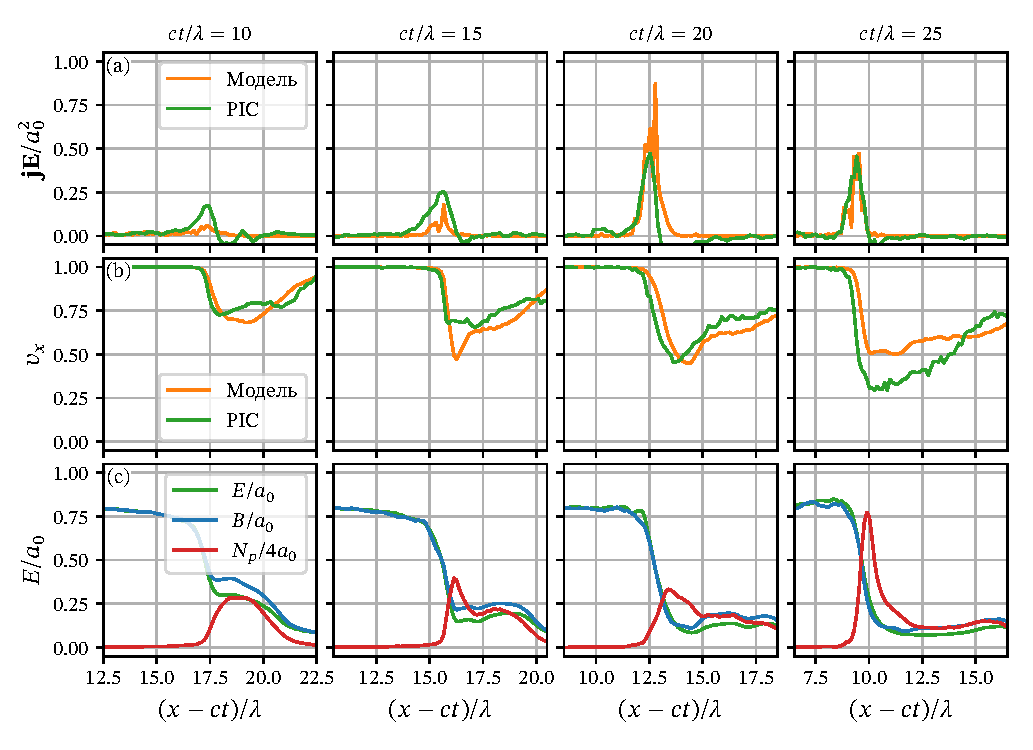
\includegraphics[width=175mm]{cushion-assumptions.pdf}}
    \caption[Проверка приближений аналитической модели развития КЭД каскада в плоской волне]{\label{fig:ch2/sec3/assumptions} 
    Проверка приближений модели. (a), (b) Значение величины $\vb{jE}$ и среднее значение скорости пар $v_x$, рассчитанные по формулам~\eqref{eq:ch2/jE} и~\eqref{eq:ch2/vx} соответственно (оранжевые линии), и взятые напрямую из результатов QED-PIC моделирования (зелёные линии) в различные моменты времени. (c) Распределение амплитуды электрического (зелёные линии) и магнитного (синие линии) полей и концентрации $e^-e^+$ плазмы (красные линии). }
\end{figure}

Предполагая, что время нахождения частицы в вакуумной области достаточно мало, поэтому реакция излучения не успевает существенно влиять на динамику частицы, будем считать, что $\chi\approx\chi_0=\text{const}$.
Тогда
\begin{equation}
    \Delta\varepsilon_\mathrm{rad} = I_\mathrm{rad}(\chi_0)\Delta\varphi.
\end{equation}
Для вычисления величины $\Delta\varphi$ воспользуемся выражениями~\eqref{eq:ch2/sec3/pw_vac_av} и~\eqref{eq:ch2/sec3/deltae_fin}
\begin{equation}
    \mu \varepsilon_\gamma (1 - \cos\theta) = \frac{E^2}{\varepsilon_\gamma (1 - \cos\theta)}\sin^2\frac{\Delta\varphi}{2},
\end{equation}
откуда получаем
\begin{equation}
    \Delta\varphi =  \frac{2\varepsilon_\gamma (1 - \cos\theta)}{E}\sqrt{\mu}
\end{equation}
Учитывая, что $\chi_0 = \chi_\gamma / 2$, выражение для источника $S[\varepsilon_p, \mathrm{rad}]$ записывается в следующем виде
\begin{multline}
    S[\varepsilon, \mathrm{rad}] = \frac{2 \varepsilon_\gamma n_\gamma \sqrt{\mu}}{E} \int_0^\pi \Phi(\theta, v_{\gamma\parallel}) W_\mathrm{pair}(\chi_\gamma, \varepsilon_\gamma) I_\mathrm{rad} \left( \frac{\chi_\gamma}{2} \right)(1 - \cos\theta)\sin\theta d\theta \equiv \\
    \equiv \overline{I_\mathrm{vac}} \frac{\varepsilon_\gamma n_\gamma \sqrt{\mu}}{E} .
\end{multline}

\subsection{Динамика $e^-e^+$ пар в плазменной области}
\label{sub.Pairs}

Согласно рассуждениям в подразделе~\ref{sub:ch2/sec2/Mechanism} в области плотной $e^-e^+$ плазмы в каждой точке пространства существует мгновенная система отсчёта $K'$, движущаяся со скоростью $v_x(x,t)\approx E/B$, в которой присутствует только магнитное поле.
В связи с простотой конфигурации ЭМ поля в $K'$, удобно проводить вычисления в этой системе отсчёта.
В $K'$ электроны и позитроны движутся вдоль магнитного поля со скоростью $v_B'$, а также вращаются в плоскости, перпендикулярной магнитному полю, со скоростью $v_\perp'$ (см. Рис.~\ref{fig:ch2/sec3/plasma}). 
Предположим, что частицы остаются в данной системе отсчёта ультрарелятивистскими (что подтверждается результатами QED-PIC моделирования), тогда справедливо равенство ${v_\perp'}^2+{v_B'}^2\approx1$.
Отметим, что движение заряженных частиц вдоль магнитного поля может приводить к появлению ненулевого тока, который необходимо учитывать в уравнениях Максвелла, тогда как их вращение в магнитном поле в среднем не создаёт ток, однако приводит к генерации гамма-квантов.
Вычислим значение КЭД параметра $\chi$, являющегося Лоренц-инвариантом, в $K'$
\begin{equation}
    \chi_p=\frac{v_\perp'\varepsilon_p'B'}{a_\mathrm{S}} .
\end{equation}
Величины в $K'$ могут быть вычислены по соответствующим величинам в лабораторной системе отсчёта следующим образом: $B'=B\sqrt{1-(E/B)^2}$, $\varepsilon_p'=\varepsilon_p\sqrt{1-(E/B)^2}$, где мы использовали тот факт, что средний импульс частиц вдоль оси $x$ равен $\gamma v_x$ и $v_x=E/B$.
Таким образом значение $\chi$ может быть вычислено следующим образом
\begin{equation}
    \label{eq:ch2/chip}
    \chi_e = \frac{v_\perp'\varepsilon_p E}{a_\mathrm{S}} \frac{1-v_x^2}{v_x} .
\end{equation}
В связи с вращением частиц в магнитном полем, можно предположить, что их угловое распределение в $K'$ близко к изотропному.
В таком случае, аналогично процедуре с гамма-квантами в подразделе~\ref{sub:ch2/sec3/gammas}, функция распределения пар в лабораторной системе отсчёта записывается в следующем виде
\begin{align}
    \label{eq:ch2/distr}
    f_p(t,x,\theta)=\Phi\left(\theta, v_x(x,t)\right) n_p(x,t) .
\end{align}
где $\Phi$ определяется так же, как в уравнении~\eqref{eq:ch2/Phi}
\begin{equation}
    \Phi(\theta,v) = \frac{1-v^2}{{2\left( 1 - v \cos{\theta}  \right)}^2} . \nonumber
\end{equation}
Результаты QED-PIC моделирования, представленные на Рис.~\ref{fig:ch2/sec3/ang} (c), (d) демонстрируют, что выражение~\eqref{eq:ch2/distr} является хорошей аппроксимацией для вычисления углового распределения пар.
Ниже будет показано, что величина $v_x$ может быть приближённо рассчитана из локальных значений электрического поля и концентрации плазмы.
В связи с этим, мы не пишем уравнения переноса величины $v_x$, подобно уравнению~\eqref{eq:ch2/hd_g2}.
Отметим также, что в случае пар мы пренебрегаем разницей между скоростью $v$ системы отсчёта, в которой распределение частиц является изотропным, и средней скоростью частиц $\overline{v}$, вычисленной по такому распределению, т.к. их максимальная разница не превышает $0.2$ согласно выражению~\eqref{eq:ch2/av_vx}.

\begin{figure}
    \centerfloat{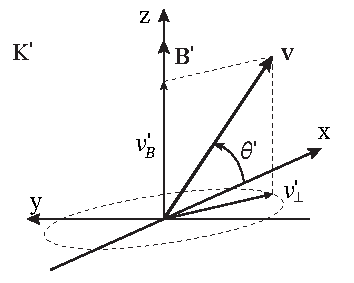
\includegraphics{cushion-plasma.pdf}}
    \caption[Геометрическое расположение скорости и магнитного поля в системе отсчёта $K'$]{\label{fig:ch2/sec3/plasma} Геометрическое расположение скорости и магнитного поля в системе отсчёта $K'$, движущейся со скоростью $v_x=E/B$.}
\end{figure}

Так как величина $\chi_p$ не зависит от угла $\theta$, то источники $S[\alpha, rad_a]$ вычисляются следующим образом
\begin{align}
    S[n, \mathrm{rad_a}] = n_p \int\limits_0^\pi \Phi(\theta, v_x) W_\mathrm{rad}(\chi_p, \varepsilon_p)  \sin\theta d\theta \equiv \overline{W_\mathrm{pl}} n_p, \\
    S[\varepsilon, \mathrm{rad_a}] =  n_p \int\limits_0^\pi \Phi(\theta, v_x) I_\mathrm{rad}(\chi_p)  \sin\theta d\theta \equiv \overline{I_\mathrm{pl}} n_p, \\
    S[v, \mathrm{rad_a}] =  n_p \int\limits_0^\pi \Phi(\theta, v_x) \cos\theta W_\mathrm{rad}(\chi_p, \varepsilon_p)  \sin\theta d\theta  \equiv \overline{W_\mathrm{pl}} v_x n_p.
\end{align}

Суммарная плотность тока частиц, усреднённая по характерному периоду Ларморовского вращения $\tau_B = \varepsilon_p/B$, вычисляется следующим образом
\begin{gather}
    \label{eq:ch2/j}
    \vb{j} = 2 n_p \frac{\vb B}{B} v_B \sqrt{1-v_x^2}, \\
    v_B = v_B' \frac{2}{\pi}\frac{\arccos{(v_x\sqrt{1-v_x^2})}}{\sqrt{1-v_x^2(1-v_x^2)}}\equiv \nu.
\end{gather}
Множитель 2 учитывает тот факт, что токи электронов и позитронов сонаправлены.
Это в свою очередь объясняется из наблюдения, что в лабораторной системе отсчета электрическое и магнитное поля нестрого перпендикулярны.
Таким образом, в системе отсчета $K'$ существует небольшое электрическое поле, направленное вдоль или против магнитного (в зависимости от знака произведения $\vb{E\cdot B}$).
Наличие этого поля приводит к тому, что средняя скорость электронов противонаправлена ему, а средняя скорость позитронов сонаправлена ему.
При этом продольный дрейф частиц не зависит от знака заряда, поэтому токи электронов и позитронов вдоль оси $x$ компенсируют друг друга, а в плоскости $yz$ суммируются.
Этот факт также указывает на то, что электрон-позитронная плазма является проводящей средой, поэтому некоторое поглощение электромагнитной энергии также происходит в этой области, хотя оно и значительно меньше, чем поглощение в вакуумной области, наблюдаемое в QED-PIC моделировании  (см. Рис.~\ref{fig:ch2/sec3/assumptions} (a)) и, таким образом, мы не учитываем его в нашей модели.
Значение $v_B$, усреднённое по частицам, которое мы обозначили как $\nu$, является вторым свободным параметром нашей модели.
Его можно грубо оценить, заметив, что для одиночной частицы значение $v_B'$ может лишь незначительно изменить своё начальное значение в связи с присутствием слабого электрического поля в $K'$.
При этом частицы входят в область плазмы после ускорения лазерным импульсом с преимущественно продольной скоростью, т.е. скоростью вдоль оси $x$, поэтому начальная проекция скорости частиц на магнитное поле, лежащее в плоскости $yz$, является маленькой величиной.
Таким образом, можно ожидать, что наша модель должна давать достоверные результаты при значениях $\nu$, близких к нулю.

Вычисление электродинамических свойства среды, отклик которой на плоскую ЭМ волну состоит в генерации тока вдоль магнитного поля, рассмотрено в следующем разделе. 
Основной вывод состоит в том, что соотношение между электрическим и магнитным полями в такой среде может быть выражено через плотность и амплитуду электрического поля следующим образом
 \begin{equation}
    \label{eq:ch2/vx}
     \frac{E}{B}=v_x=\sqrt{\frac{2}{1+\sqrt{1+\left(4n_p\nu/E \right)^2}}} .
 \end{equation}
Справедливость выражения~\eqref{eq:ch2/vx} также подтверждается путём прямого сравнения с результатами QED-PIC моделирования, продемонстрированного на Рис.~\ref{fig:ch2/sec3/assumptions} (b).


\subsection{Электродинамические свойства $e^-e^+$ плазмы}
\label{app.Electrodynamics}

Рассмотрим распространение плоской циркулярно-поляризованной ЭМ волны вдоль оси $x$ в слабо неоднородной (также вдоль оси $x$) среде, отклик которой на эту волну заключается в генерации тока $\vb{j}=2n_p\vb{v}$, <<опережающего>> электрическое поле волны на половину периода.
Для этого запишем уравнения Максвелла
\begin{align}
    \label{eq:ch2/B.Maxwell1}
    &\pdv{ E_z}{ x} = \pdv{ B_y}{ t}, \\
    \label{eq:ch2/B.Maxwell2}
    &\pdv{ E_y}{ x} = -\pdv{ B_z}{ t}, \\
    \label{eq:ch2/B.Maxwell3}
    &\pdv{ B_z}{ x} = -\pdv{ E_y}{ t} - 2 n_p v_y, \\
    \label{eq:ch2/B.Maxwell4}
    &\pdv{ B_y}{ x} = \pdv{ E_z}{ t} + 2 n_p v_z.
\end{align}
Перейдём к следующим комплексным переменным
\begin{align}
    &\epsilon=E_y+iE_z, 
    \label{eps} \\
    &\beta=B_z-iB_y, \\
    &v_y+iv_z=\frac{\epsilon}{|\epsilon|}iv_{\perp} ,
\end{align}
Введём также вектор-потенциал $a$ следующим образом
\begin{equation}
    \epsilon=-\pdv{ a}{ t} \text{, } \beta=\pdv{ a}{ x}.
\end{equation}
В новых переменных уравнения~\eqref{eq:ch2/B.Maxwell1}--\eqref{eq:ch2/B.Maxwell4} переписываются в следующем виде
\begin{equation}
    \pdv[2]{ a}{ x}=\pdv[2]{ a}{ t}-2 n_p \pdv{ a}{ t}\left| \pdv{ a}{ t} \right|^{-1} iv_\perp.
\end{equation}
Будем искать решение этого уравнения в виде монохроматической плоской волны с амплитудой, зависящей от координаты $x$
\begin{equation}
    a=E(x)e^{i\int^{x}\kappa(x)dx-it},
    \label{a}
\end{equation}
где $E(x)$ и $\kappa(x)$~---~действительные функции координаты $x$, имеющие смысл амплитуды и волнового числа волны.
В итоге уравнения имеют следующий вид
\begin{align}
    \label{eq:ch2/B.Cushion1}
    \pdv[2]{ E}{ x}+E(1-\kappa^2)+2 n_p v_{\perp} =0, \\
    \label{eq:ch2/B.Cushion2}
    E \pdv{ \kappa}{ x} + 2\kappa \pdv{ E}{ x} = 0.
\end{align}
Если плазма является слабо неоднородной, то можно применить приближение ВКБ для решения данного уравнения.
Предполагая, что масштаб неоднородности плазмы $L$ существенно превышает длину волны $\lambda$, можно пренебречь слагаемыми со второй производной: $\partial^2E/\partial x^2 \sim E/L^2 \ll \kappa^2 E = (2\pi)^2E/\lambda^2$.
В таком случае имеем
\begin{equation}
    E(1-\kappa^2)+2 n_p v_{\perp} = 0.
\end{equation}
Решая это уравнение, получаем
\begin{equation}
    \label{eq:ch2/B.kappa}
    \kappa \equiv \frac{B}{E}=\sqrt{1+\frac{2 n_p v_{\perp}}{E}},
\end{equation}
Воспользуемся выражением~\eqref{eq:ch2/j} для $v_\perp$, т.е.
\begin{equation}
v_\perp = \nu \sqrt{1-v_x^2}.
\label{vp}
\end{equation}
Отметим, что в случае $\nu>0$ согласно~\eqref{eq:ch2/B.kappa}, $B>E$, и поэтому $1/\kappa$ имеет смысл дрейфовой скорости $v_x$.
Таким образом,
\begin{equation}
    \frac{1}{v_x}=\sqrt{1+\frac{2n_p\nu}{E}\sqrt{1-v_x^2}} .
\end{equation}
Решение данного уравнения имеет следующий вид
\begin{gather}
    \label{eq:ch2/B.vx}
    v_x= {\left( \frac{2}{1+\sqrt{1+S^2}} \right)}^{1/2},\\
    S=\frac{4n_p\nu}{E}.
\end{gather}
Сравнение полученного решения с численным решением уравнений~\eqref{eq:ch2/B.Cushion1}--\eqref{eq:ch2/B.Cushion2} продемонстрировано на Рис.~\ref{fig.ch2/sec3/ED} как в случае применимости, так и неприменимости приближения ВКБ.
Решение~\eqref{eq:ch2/B.vx} получено в предположении, что $v^2 = 1$, таким образом полученное оно справедливо в системе отсчёта, где частицы являются ультрарелятивистскими, в частности в лабораторной системе отсчёта. 

\begin{figure}
	\centerfloat{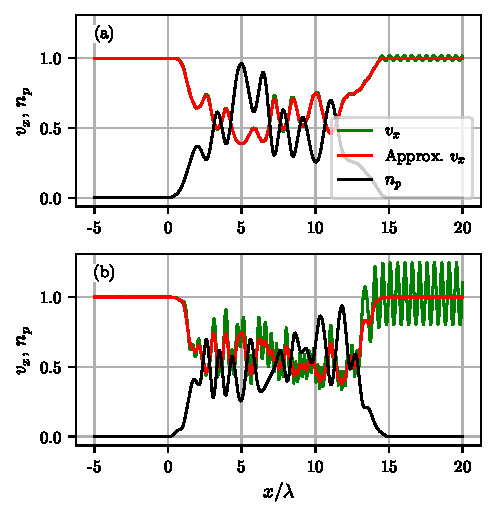
\includegraphics{cushion-ED.pdf}}
	\caption[Дрейфовая скорость частиц в электрон-позитронной плазме]{\label{fig.ch2/sec3/ED} 
    \fixme{Дрейфовая скорость $v_x=E/B$, рассчитанная из численного решения уравнений~\eqref{eq:ch2/B.Cushion1}--\eqref{eq:ch2/B.Cushion2} (зелёная линия) и с помощью аналитического выражения~\eqref{eq:ch2/B.vx} (красная линия) для случайно-неоднородного распределения плазмы (чёрная линия). Масштаб неоднородности превышает длину волны на подрисунке (а), что делает приближение ВКБ справедливым, и меньше её на подрисунке (b).}}
\end{figure}

\subsection{Формулировка модели и сравнение с QED-PIC моделированием}
\label{sub:ch2/sec3/Discussion}

Последние оставшиеся неопределёнными величины~---~это параметры $\psi_\mathrm{vac}$ и $\psi_\mathrm{pl}$, которые разделяют в пространстве вакуумную и плазменную области.
Отметим, что по продольной скорость пар $v_x$, определяемой согласно уравнению~\eqref{eq:ch2/vx}, можно легко различить эти области: в вакууме $v_x\approx 1$, тогда как в плазменной области $v_x < 1$.
Поэтому можно выбрать $\psi_\mathrm{vac}$ и $\psi_\mathrm{pl}$ следующим образом
\begin{align}
    \psi_\mathrm{vac} = v_x^M \\
    \psi_\mathrm{pl} =  1 - v_x^M
\end{align}
где $M\sim 10$~---~достаточно большая константа.
Значение данной константы подбирается исходя из некого условного порога величины $v_x$, при превышении которого можно предположить, что плазма достаточно редкая и и коллективными эффектами можно пренебречь.
Далее будем полагать, что данный порог соответствует величине $0.7$, и $M=8$.

Таким образом, уравнения, описывающие развитие КЭД каскада в плоской волне, имеют следующий окончательный вид
\begin{align}
    \label{eq:ch2/fin1}
    \frac{\partial }{\partial t}n_p  +\frac{\partial}{\partial x}\left( v_x n_p \right) &= \overline{W_\mathrm{pair}} n_\gamma  ,\\
    \label{eq:ch2/fin2}
    \phantom{abs} &= 
    \begin{multlined}[c]
        \mathllap{\frac{\partial}{\partial t}\left( \varepsilon_p n_p \right)  + \frac{\partial}{\partial x}\left( v_p \varepsilon_p n_p \right) \quad}
        \overline{W_\mathrm{pair}} n_\gamma \frac{\varepsilon_\gamma}{2}  + \\
        + n_\gamma\varepsilon_\gamma  \mu \left( \overline{G_\mathrm{rad}} - \frac{\overline{I_\mathrm{vac}}}{\sqrt{\mu} E}  \right) \psi_\mathrm{vac} - \overline{I_\mathrm{pl}} n_p \psi_\mathrm{pl} ,
    \end{multlined} \\
    \label{eq:ch2/fin3}
    \frac{\partial }{\partial t}n_\gamma  +\frac{\partial}{\partial x}\left( \overline{v_{\gamma\parallel}} n_\gamma \right)&=-\overline{W_\mathrm{pair}} n_\gamma + 2\overline{W_\mathrm{rad}} n_p \psi_\mathrm{pl} ,\\
    \label{eq:ch2/fin4}
    \frac{\partial}{\partial t}\left( \overline{v_{\gamma\parallel}} n_\gamma \right) + \frac{\partial}{\partial x}\left( \overline{v_{\gamma\parallel}^2} n_\gamma \right) &= -\overline{V_\mathrm{pair}} n_\gamma + 2 \overline{V_\mathrm{rad}} n_p \psi_\mathrm{pl} ,\\
    \label{eq:ch2/fin5}
    \frac{\partial}{\partial t}\left( \varepsilon_\gamma n_\gamma \right) +\frac{\partial}{\partial x}\left( \overline{v_{\gamma\parallel}} \varepsilon_\gamma n_\gamma \right) &=-\overline{W_\mathrm{pair}}n_\gamma\varepsilon_\gamma   +2 \overline{I_\mathrm{pl}} n_p \psi_\mathrm{pl} ,\\
    \label{eq:ch2/fin6}
    \frac{\partial }{\partial t}\left( \frac{E^2 + E^2/v_x^2}{2} \right) +\frac{\partial}{\partial x} \left( \frac{E^2}{v_x} \right) &=  -2\mu E^{2/3}\varepsilon_\gamma^{1/3}\overline{G_\mathrm{rad}} n_\gamma\psi_\mathrm{vac}  ,\\
    \label{eq:ch2/fin7}
    \frac{\partial }{\partial t}\Sigma_\gamma &=  \overline{I_\mathrm{vac}} n_\gamma \psi_\mathrm{vac} .
\end{align}

Отметим, что в нашей модели сохраняется полная энергия, т.е.
\begin{equation}
    \int \left( 2n_p\varepsilon_p + n_\gamma \varepsilon_\gamma + \frac{E^2 + B^2}{2} \right) dx + \Sigma_\gamma = \text{const} .
\end{equation}


\subsection{Аналитические оценки}
\label{sub:ch2/sec3/analytics}
Перед переходом к численному решению данных уравнений и сравнению в результатами QED-PIC моделирования, сделаем некоторые очень грубые, но аналитические оценки.
\fixme{Мы будем предполагать, что электроны и позитроны излучают гамма-кванты строго против оси $x$.
% Эти гамма-фотоны в свою очередь с вероятностью $W_\mathrm{pair}$ могут распадаться на пары.
Распределение лазерной интенсивности будем считать постоянным и однородным.
В связи с последним предположением, вероятности $W_\mathrm{pair}$ и $W_\mathrm{rad}$ также будем считать постоянными величинами.
В таком случае уравнения непрерывности для концентрации плазмы $n_p$ и фотонов $n_\gamma$ записываются следующим образом в системе отсчёта, движущейся со скоростью $v_x$:}
\begin{align}
	\label{dnpdt}
    \pdv{n_{p}}{ t}  & =    W_\mathrm{pair}n_{\gamma}, \\
	\label{dngdt}   
    \pdv{ n_{\gamma}}{ t}-\pdv{ n_{\gamma}}{ x} &  =   -W_\mathrm{pair}n_{\gamma}+2W_\mathrm{rad}n_{p}
\end{align}
Если пренебречь в \eqref{dngdt} слагаемым с $\partial_x$, характеризующим пространственную дисперсию, то уравнения непрерывности переходят в уравнения, описывающие КЭД каскад во вращающемся электрическом поле без пространственной динамики~\cite{bashmakov2014effect,grismayer2017seeded}.
Уравнения~\eqref{dnpdt}--\eqref{dngdt} можно решить с помощью одностороннего преобразования Фурье \cite{LL10}, т.е. разложения решения на сумму экспонент с действительными значениями $k$ и комплексными значениями $\omega$:
\begin{equation}
    \label{t-x}
    n_{p,\gamma}\left(t,x\right) = \intop_{-\infty+i\sigma}^{+\infty+i\sigma}\mathrm{e}^{-i\omega t}\frac{d\omega}{2\pi}\intop_{-\infty}^{+\infty}\mathrm{e}^{ikx}n_{p,\gamma}\left(\omega,k\right)\frac{\dd k}{2\pi}.
\end{equation}
где
\begin{equation}
    \label{w-k}
n_{p,\gamma}\left(\omega,k\right) = \intop_{0}^{+\infty}\mathrm{e}^{i\omega t}dt\intop_{-\infty}^{+\infty}\mathrm{e}^{-ikx}n_{p,\gamma}\left(t,x\right)\dd x,
\end{equation}
и $\sigma$~---~такое действительное число, что контур интегрирования лежит в области аналитичности $n_{p,\gamma}$. 
Для начальных распределений плотности плазмы и гамма-квантов равных 
$n_{p}\left(0,x\right)$ и $n_{\gamma}\left(0,x\right)$ соответственно, решение находится следующим образом:
\begin{equation}
    \label{np}
    n_{p}\left(t,x\right) = \intop_{-\infty+i\sigma}^{+\infty+i\sigma}\frac{\dd\omega}{2\pi}\intop_{-\infty}^{+\infty}\frac{\dd k}{2\pi}\intop_{-\infty}^{+\infty}dx' 
    \frac{W_\mathrm{pair}n_{p}(0,x')+i\left(\omega+k\right)n_{\gamma}(0,x')}{\Delta\left(\omega,k\right)} \mathrm{e}^{ik(x-x')-i\omega t}
\end{equation}
где $\Delta\left(\omega,k\right)=\omega^{2}+\omega(k + iW_\mathrm{pair})+2W_\mathrm{pair}W_\mathrm{rad}$. 
Возмущения начального распределения распространяются вдоль характеристик, определяемых дисперсионным уравнением $\Delta\left(\omega,k\right)=0$, имеющим следующее решение: 
\begin{equation}
    \label{dispersion}
    \omega=\frac{-k-i W_\mathrm{pair} \pm\sqrt{(k+i W_\mathrm{pair})^{2}-8 W_\mathrm{pair}W_\mathrm{rad}}}{2}. 
\end{equation}
Групповая скорость этих возмущений равна $v_\mathrm{gr}=\partial\mathrm{Re}[\omega]/\partial k$. 
Анализ дисперсионного соотношения показывает, что возмущения с малыми волновыми числами ($k\ll W_\mathrm{pair}$) наиболее неустойчивы и обладают следующим инкрементом неустойчивости:
\begin{equation}
    \Gamma \equiv \mathrm{Im}\left[\omega\right] =\frac{W_\mathrm{pair}}{2} \left(\sqrt{1+\frac{8 W_\mathrm{rad}}{W_\mathrm{pair}}}-1\right),
    \label{gamma}
\end{equation}
что совпадает с инкрементом неустойчивости КЭД каскада во вращающемся электрическом поле~\cite{bashmakov2014effect,grismayer2017seeded}. 
Из~\eqref{dispersion} получим дисперсионное соотношение для неустойчивых возмущений:
\begin{align}
    \omega & \approx  \frac{\mu-1}{2}k + i\Gamma \\
    \mu & =  \frac{1}{\sqrt{1+8 W_\mathrm{rad}/W_\mathrm{pair}}}.
    \label{omega}
\end{align} 
В пределе $a_0 \rightarrow \infty$, $W_\mathrm{rad}/W_\mathrm{pair} \approx 4$ и $\mu \approx0.17$ \cite{berestetskii1982quantum}. 
Поэтому возмущения с малыми волновыми числами распространяются со скоростью ${v_\mathrm{gr}\approx -0.41}$.
Это значение совпадает с результатами численного решения уравнений~\eqref{dnpdt}--\eqref{dngdt} с различными формами начальных распределений пар и гамма-квантов (см. пример такого решения на Рис.~\ref{front}).

\begin{figure}[h!]
	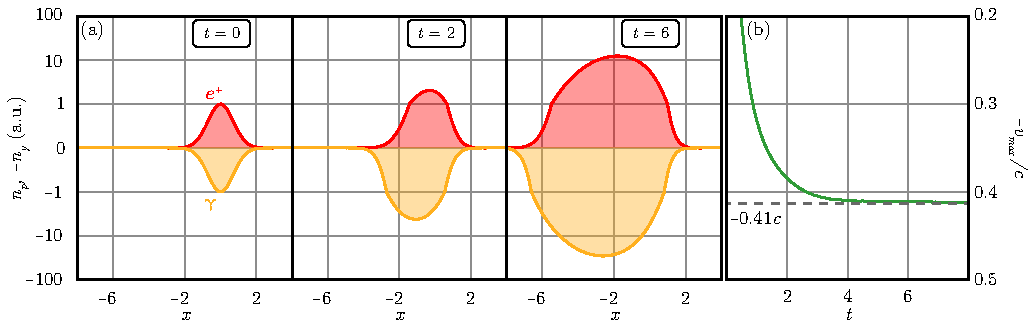
\includegraphics[width=165mm]{front.pdf}
    \caption{\label{front} \fixme{Численное решение уравнений (\ref{dnpdt})--(\ref{dngdt}): (a) Распределение плотности позитронов $n_p$ (красная линия) и гамма-квантов $n_\gamma$ (оранжевая линия) в различные моменты времени. Масштаб вертикальной оси линейный для значений $[-1,1]$ и логарифмический для остальных значений. Координаты, время и плотности нормированы таким образом, что $W_\mathrm{rad}=1.0$, $W_\mathrm{pair}=0.25$.
    (b) Скорость фронта распределения плотности $n_p$, определяемая по порогу $n_p = 0.1$, как функция времени.}}
\end{figure}

В системе отсчёта, движущейся со средней продольной скоростью плазмы, скорость фронта каскада $v_\mathrm{fr}$ совпадает с найденной групповой скоростью $v_\mathrm{gr} \approx -0.41$.
Переход в лабораторную систему отсчёта позволяет связать среднюю продольную скорость частиц плазмы и скорость фронта каскада:
\begin{equation}
    v_\mathrm{fr}=\frac{v_\mathrm{pl}+v_\mathrm{gr}}{1+ v_\mathrm{pl} v_\mathrm{gr} /c^2} 
\label{vcf}
\end{equation}
Решая это уравнение относительно $v_\mathrm{pl}$ получаем:
\begin{equation}
    \label{vpl}
    v_\mathrm{pl}=\frac{v_\mathrm{fr}-v_\mathrm{gr}}{1-v_\mathrm{gr}v_\mathrm{fr}/c^2} 
\end{equation}
Эти рассуждения предсказывают $v_\mathrm{pl}=0.61$ для $v_\mathrm{fr} = 0.27$ ($a_{0}=2500$, см. Рис.~\ref{fig:ch2/cushion-x-t}), что достаточно близко к усреднённой скорости позитронов $\approx 0.75$, полученной из численного моделирования (см. Рис.~\ref{fig:ch2/field-structure}(b)).

\subsection{Численное решение}
\label{sub:ch2/sec3/Numeric}

Численное решение уравнений~\eqref{eq:ch2/fin1}--\eqref{eq:ch2/fin6} находится по методу линий: частные производные $\partial/\partial x$ аппроксимируются конечными разностями для получения системы ОДУ, которая решается с помощью явного метода Рунге-Кутты.
Так как метод Рунге-Кутты не является симплектическим, то сохранение энергии на каждом шаге интегрирования соблюдается путем отсечения производной $\partial n_\gamma /\partial t$ так, чтобы полная энергия не росла.
Относительная ошибка, полученная в результате этой процедуры, оказывается приемлемо малой.
Свободные параметры оценивались вручную путем сравнения решения с результатами трехмерного QED-PIC моделирования на основе двух макроскопических параметров: скорости фронта каскада и энергетического баланса в системе.
После тестирования редуцированной модели выяснилось, что существует положительная корреляция между параметром $\nu$ и скоростью распространения фронта каскада.
Параметр $\mu$ в основном определяет передачу энергии от лазера к каскадным частицам, поэтому, изменяя этот параметр, можно управлять характерным временем исчерпания энергии лазера.
Отметим, что расчетные значения параметров подгонки практически равны друг другу для различных начальных условий (см. рис.~\ref{fig:ch2/sec3/sol2500}--\ref{fig:ch2/sec3/sol1000}).

Трехмерное QED-PIC моделирование было выполнено с использованием кода QUILL~\cite{QUILL}, который позволяет моделировать КЭД эффекты с помощью метода Монте-Карло.
Начальное распределение ЭМ полей имеет вид плоской волны с длиной волны $\lambda=2\pi c/\omega_{L}=\SI{1}{\um}$ и амплитудой $a_0 $, распространяющееся вдоль оси $x$ с пространственно-временной огибающей, задаваемой следующим выражением
\begin{equation}
a(x,y,z) =  \cos^2 \left( \frac{ \pi }{2}   \frac{x^4}{\sigma_x^4 } \right) \cos^2 \left( \frac{ \pi}{2}   \frac{\left( y^2 + z^2 \right)^2}{\sigma_r^4 } \right)
\end{equation}
Поперечный пространственный размер лазерного импульса составлял $2\sigma_r = \SI{18}{\um}$, а длительность импульса $\SI{60.5}{\femto\second}$ ($2\sigma_x = \SI{18.15}{\um}$).
Размер области модулирования составлял $30\lambda\times 30\lambda\times 30\lambda$, количество ячеек $3000\times 300\times 300$.
Как обсуждалось в подразделе~\ref{sub:ch2/sec2/Mechanism}, финальная стадия развития каскада КЭД в одиночном лазерном импульсе практически не зависит от затравки, поэтому мы выбираем затравку в виде короткого гамма-сгустка, распространяющегося навстречу лазерного импульса, чтобы не учитывать взаимодействие с электрон-ионной плазмой, существенно отличающейся от формирующейся электрон-позитронной плазмы.
Начальная затравка в таком виде в нашей модели может быть задана путём инициализации $v_{\gamma\parallel}(t=0)\approx-1$.
Распределения плотности в нашей модели и PIC-моделировании совпадают и выражаются следующей формулой: $n_\gamma(t=0)=n_0\max\left\{0, 1 - (x-x_0)^2/w_\gamma ^2 \right\}$, где $w_\gamma$~---~полуширина сгустка, а $x_0$~---~положение его центра.
Начальная энергия гамма-квантов была установлена равной $200 m_e c^2$.

\begin{figure}
    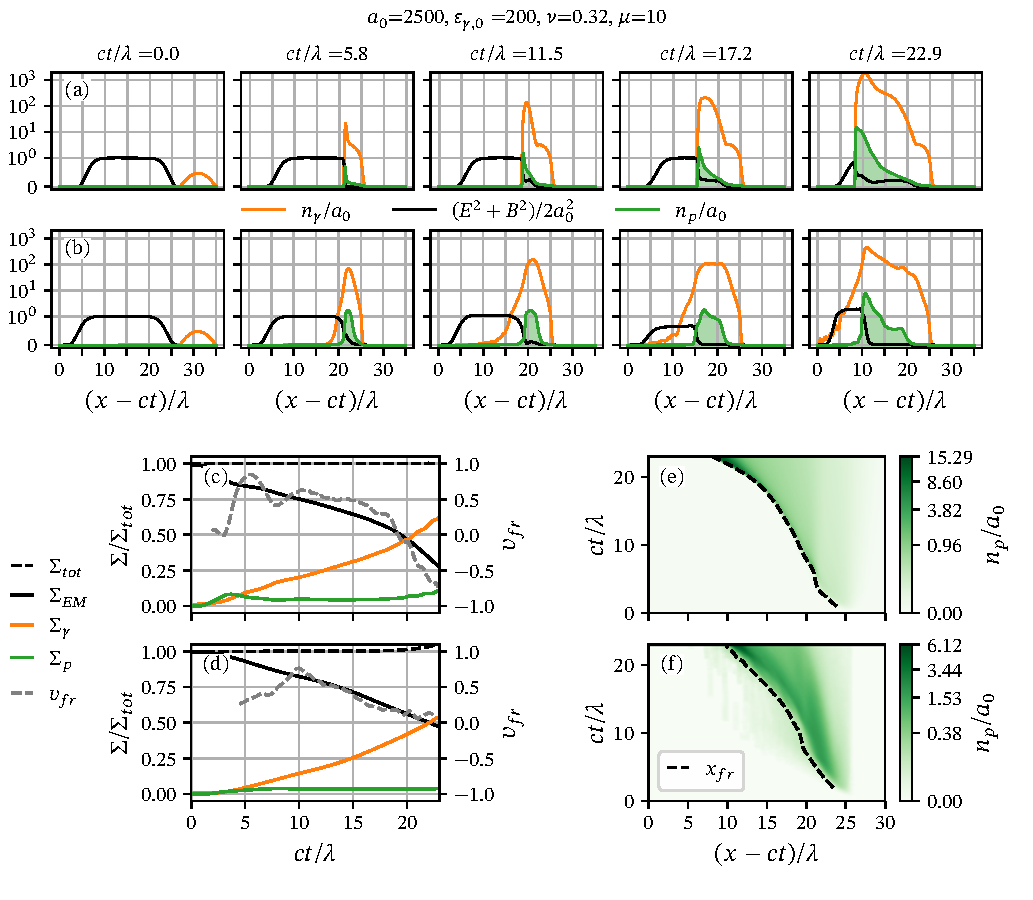
\includegraphics{cushion-sol-2500-new.pdf}
    \caption[Сравнение решения модельных уравнений, описывающий развитие КЭД каскада и результатов QED-PIC моделирования для начальных параметров $a_0=2500$, $n_{\gamma,0}=0.5 a_0 n_\mathrm{cr}$]{\label{fig:ch2/sec3/sol2500} 
    Сравнение между (a, c, e) решением уравнений~\eqref{eq:ch2/fin1}--\eqref{eq:ch2/fin6} и (b, d, f) результатами QED-PIC моделирования для начальных параметров $a_0=2500$, $n_{\gamma,0}=0.5 a_0 n_\mathrm{cr}$.
    (a, b) Распределение концентрации гамма-квантов $n_\gamma$, плотности ЭМ энергии $(E^2+B^2)/2$ и концентрации плотности плазмы $n_p$ в различные моменты времени.
    Вертикальная шкала является линейной в диапазоне $[0,\ 1]$ и логарифмической в диапазоне $[1,\ +\!\infty]$.
    (c, d) Баланс энергии в системе: полная энергия $e^-e^+$ пар $\Sigma_p$, гамма-квантов $\Sigma_\gamma$ и ЭМ энергия $\Sigma_{EM}$, нормированные на полную начальную энергию системы $\Sigma_{tot}$; скорость фронта каскада $v_\mathrm{fr}$.
    (e, f) Распределение $e^-e^+$ пар в плоскости $x$, $t$ и положение фронта каскада $x_\mathrm{fr}$. Значения свободных параметров модели: $\nu=0.32$, $\mu=10$.}
\end{figure}

Прямое сравнение между решениями уравнений ~\eqref{eq:ch2/fin1}~--~\eqref{eq:ch2/fin6} и результатами QED-PIC моделирования показано на Рис.~\ref{fig:ch2/sec3/sol2500}~--~\ref{fig:ch2/sec3/sol1000}.
Наша модель качественно совпадает с результатами QED-PIC моделирования с точки зрения распределения частиц и электромагнитного поля, а также энергетического баланса.
Также отчетливо различаются режимы развития каскада как в нашей модели, так и в QED-PIC моделировании.

Первый режим реализуется, когда значение $a_0$ лазерного импульса недостаточно велико или гамма-сгусток недостаточно плотный.
В этом случае плотность образующейся электрон-позитронной плазмы не достигает релятивистской критической плотности, так что $v_x\approx 1$, т.е. не возникают коллективные плазменные эффекты.
В этом случае плазменная область вообще отсутствует, а вновь рождающиеся частицы движутся в неизменном поле лазерного импульса, близком к плоской волне.
Как обсуждалось в работах~\cite{di2012extremely, bulanov2013electromagnetic, narozhny2015quantum, mironov2017observable} (\fixme{в главе 1}), в этом случае значение параметра $\chi$ пар не растет при движении в плоской волне.
Но после каждого акта испускания гамма-кванта величина $\chi$ делится между родительской и дочерней частицами, так что через несколько поколений $\chi$ всех частиц становится пренебрежимо малым и развитие каскада прекращается.
Таким образом, при достаточно малых $a_0$ гамма-кванты гамма-сгустка распадаются на пары, оставляющие <<шлейф>> электронов и позитронов, которые ускоряются вперед и распространяются вместе с лазерным импульсом.
Хотя плотность плазмы мала, общее количество пар может быть достаточно большим, чтобы значительная часть лазерной энергии передавалась им (см. Рис.~\ref{fig:ch2/sec3/sol1000} (c), (d) ).
Поскольку в этом режиме все частицы распространяются независимо друг от друга, фронт каскада распространяется с почти постоянной скоростью $v_\mathrm{fr}\approx -0.5$.

\begin{figure}[ht]
    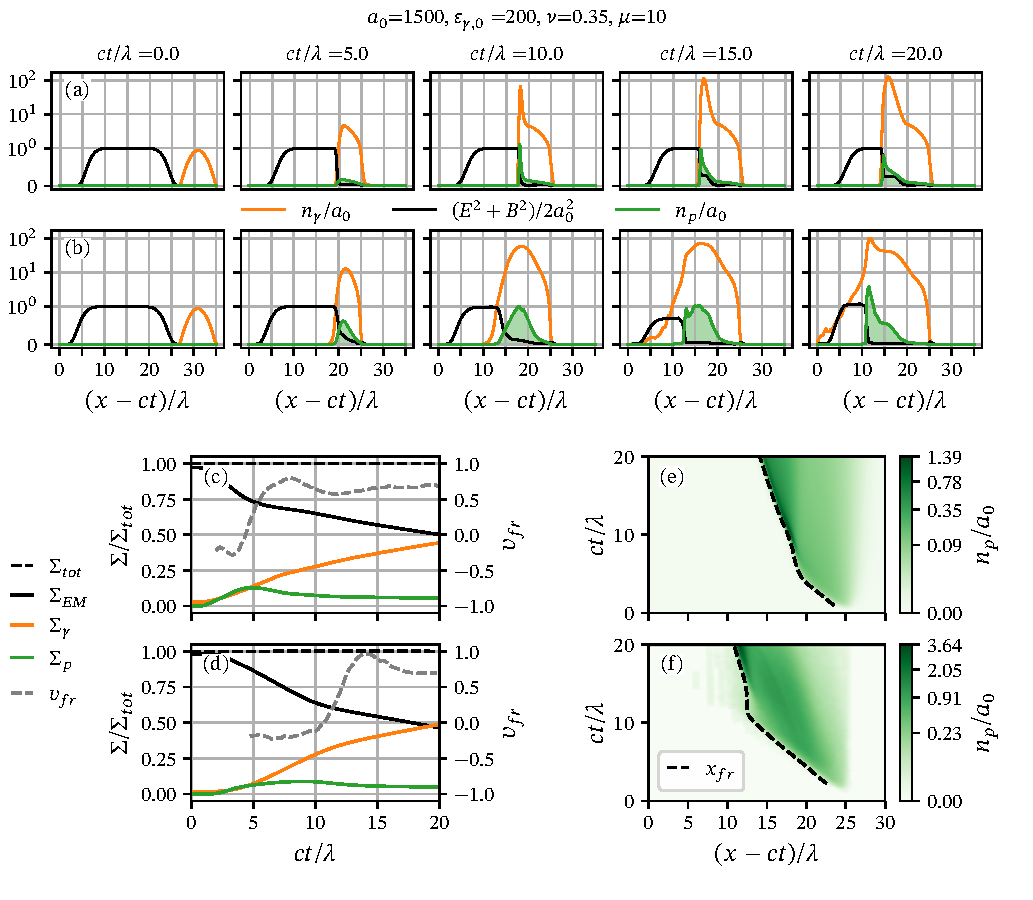
\includegraphics{cushion-sol-1500-new.pdf}
    \caption[То же, что на Рис.~\ref{fig:ch2/sec3/sol2500} для начальных параметров $a_0=1500$, $n_{\gamma,0}=a_0 n_\mathrm{cr}$]{\label{fig:ch2/sec3/sol1500} 
    То же, что на Рис.~\ref{fig:ch2/sec3/sol2500} для начальных параметров $a_0=1500$, $n_{\gamma,0}=a_0 n_\mathrm{cr}$. Значения свободных параметров модели: $\nu=0.35$, $\mu=10$.}
\end{figure}

% The first regime is observed when $a_0$ of the laser pulse is not big enough or the gamma-bunch is not dense enough. In that case the density of the produced electron-positron plasma does not reach the relativistic critical density so that $v_x\approx 1$, i.e. the collective plasma effects do not occur. In this case the plasma region is not present at all and the newly born particles move in the unaltered field of the laser pulse which is close to the plane wave. As discussed in~\cite{DiPiazza2012, bulanov2013electromagnetic, narozhny2015quantum, mironov2017observable} in that case $\chi$ of the pairs does not grow during its motion in the plane wave. But after each act of the gamma-quant emission it splits between the parent and the child particles so after few generations $\chi$ of all the particles becomes negligibly small so the cascading ceases. Thus for small enough $a_0$ the gamma-quanta of the gamma-bunch decay into pairs levaing the `trail' of the electrons and positrons which are accelerated forwards and co-propagate with the laser pulse. Although the density of the plasma is small the total number of the pairs can be big enough so that the significant portion of the laser energy is transferred to them [see Fig.~\ref{fig:ch2/sec3/sol1000} (c), (d)]. Because in this regime all the particles propagate independently to each other the cascade front propagates with almost constant velocity $v_\mathrm{fr}\approx -0.5$.

Во втором режиме каскад развивается, как обсуждалось в подразделе~\ref{sub:ch2/sec2/Mechanism}.
Пик плотности пар распространяется в сторону лазера со значительно меньшей скоростью (относительно переднего фронта лазерного импульса), чем в первом режиме.
При этом плотность плазмы растет во времени в отличие от первого режима, когда плотность плазмы в каждой точке остается практически неизменной после прохождения этой точки начальным гамма-сгустком.
Как упоминалось в п.~\ref{sub.Pairs}, плотная электрон-позитронная плазма фактически почти не поглощает лазерное поле, поэтому, несмотря на то, что в этом режиме общее число пар значительно больше, чем в первом скорости передачи энергии от ЭМ поля к парам близки друг к другу в обоих режимах.

% In the second regime the cascade develops as discussed in Sec.~\ref{sec.Introduction}. The peak of the pairs density propagates towards the laser with a much slower velocity (relative to the leading edge of the laser pulse) than in the first regime. Moreover the density of the plasma grows in time in contrast to the first regime where the plasma density at each point stays almost the same after the initial gamma-bunch passes that point. As mentioned in Sec.~\ref{sub.Pairs} the dense electron-positron plasma actually almost does not absorb the laser field that is why despite the fact that in this regime the total number of the pairs is much larger than in the first regime, the rates of the energy transfer from the EM field to the pairs are close to each other in both regimes.

\begin{figure}[ht]
    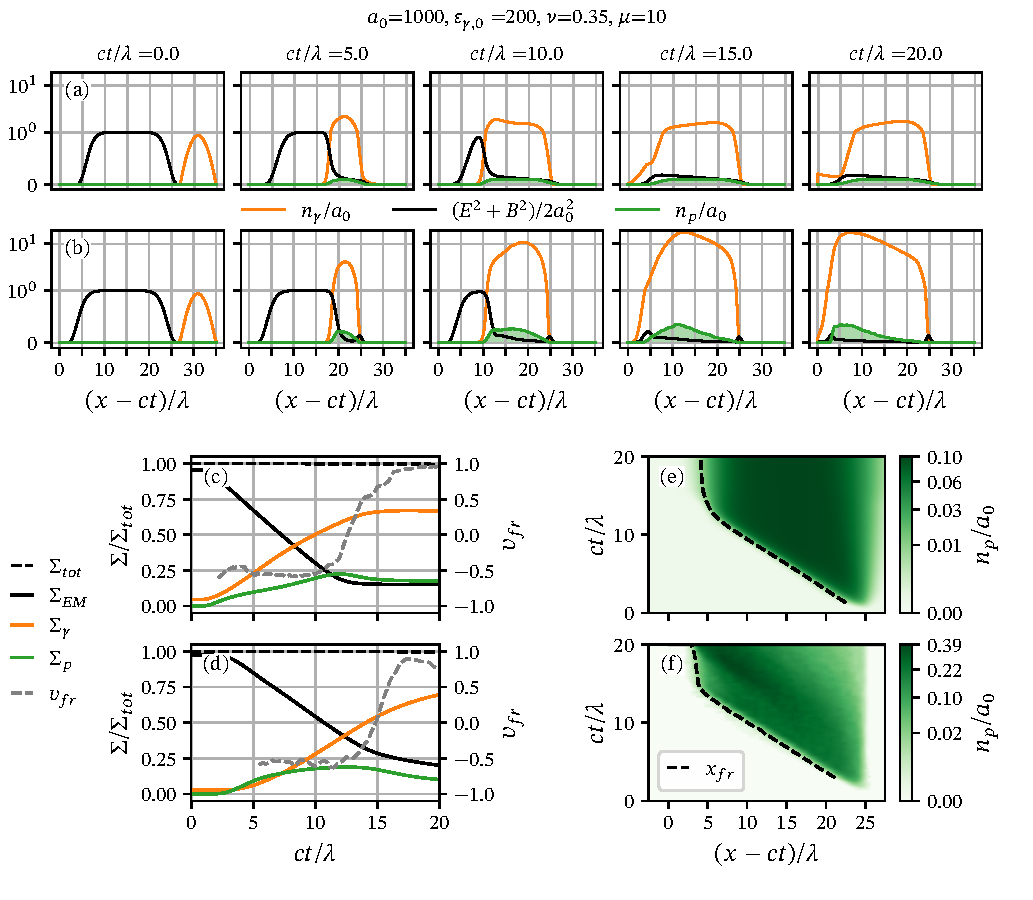
\includegraphics{cushion-sol-1000-new.pdf}
    \caption[То же, что на Рис.~\ref{fig:ch2/sec3/sol2500} для начальных параметров $a_0=1000$, $n_{\gamma,0}=a_0 n_\mathrm{cr}$]{\label{fig:ch2/sec3/sol1000} 
    То же, что на Рис.~\ref{fig:ch2/sec3/sol2500} для начальных параметров $a_0=1000$, $n_{\gamma,0}=a_0 n_\mathrm{cr}$. Значения свободных параметров модели: $\nu=0.35$, $\mu=10$.}
\end{figure}

Если $a_0$ лежит между значениями, при которых наблюдается либо первый, либо второй режим, то на начальном этапе каскад напоминает каскад S-типа, на что явно указывает отрицательное значение скорости фронта каскада (см. синюю пунктирную линию на Рис.~\ref{fig:ch2/sec3/sol1500} (c), (d)). 
В какой-то момент плотность пар становится достаточно большой, чтобы изменить распространение лазера и каскад переходит в режим самоподдержания.
На смену этих двух режимов указывает резкое изменение скорости фронта каскада.
Начальная стадия (стадия каскада S-типа) просматривается и при больших значениях $a_0$ (см. рис.~\ref{fig:ch2/sec3/sol2500}), однако она значительно короче и слабо выражена в результатах QED-PIC моделирования.

% If the $a_0$ lays in-between the values of $a_0$ at which either the first or the second regime is observed, at the initial stage the cascade resembles the S-type cascade which is clearly indicated by the negative value of the velocity of the cascade front [see grey dashed line in Fig.~\ref{fig:ch2/sec3/sol1500} (c), (d)]. At some point the density of the pairs becomes large enough to alter the laser propagation and to shift the cascade dynamics to the self-sustained regime. The change between these two regimes is indicated by abrupt change in the velocity of the cascade front. The initial stage (stage of the S-type cascade) can also be seen for larger values of $a_0$ (see Fig.~\ref{fig:ch2/sec3/sol2500}), though it is much shorter and is hardly pronounced in the results of the QED-PIC simulations.

\fixme{Мы также проверили разработанную выше грубую аналитическую оценку, из которой была получена связь между средней продольной скоростью частиц каскада и скоростью фронта каскада.}
Это предсказание модели, рассчитанное на основе средней скорости частиц каскада, примерно совпадает с реальной скоростью, наблюдаемой в модельном решении (см. Рис.~\ref{fig.former}) на стадии самоподдержания каскада.
Поскольку этот этап никогда не начинается при $a_0 = 1000$, эта упрощенная модель не может быть применена в этом случае.

% We also verified the results of the simplified model developed by us in Ref.~\cite{Samsonov2019} from which a relation between the mean longitudinal velocity of the cascade particles and the cascade front velocity was obtained. This model prediction calculated based on the mean velocity of the cascade particles roughly coinsides with the actual velocity observed in the model solution (see Fig.~\ref{fig.former}) at the stage of the cascade self sustenance. As this stage never starts for $a_0 = 1000$, this simplified model cannot be applied in that case.

Стоит отметить некоторые особенности развития КЭД каскада не воспроизводятся в нашей модели.
Например, в PIC моделировании отчетливо виден <<хвост>> пространственного распределения гамма-квантов, распространяющийся навстречу лазерному импульсу.
Эти гамма-кванты имеют относительно низкую энергию и, следовательно, не могут фотообразовать электрон-позитронные пары.
Наша модель предсказывает, что края распределения плазмы и гамма-квантов почти полностью совпадают.
Суммарная энергия, уносимая такими гамма-квантами, незначительна, поэтому для развития каскада эта особенность не является решающей.
Причина, по которой наша модель не может отразить эту особенность, заключается в том, что мы предполагаем, что функции распределения являются моноэнергетическими.
Более высокую точность можно получить, если разбить гамма-кванты на несколько групп с разными энергиями и описать их отдельно; тогда эта особенность присутствовала бы в наших решениях.
Но, как уже упоминалось в п.~\ref{sub:ch2/sec3/Assumptions}, это сильно усложнит модель, но не приведет к существенным качественным изменениям решений.
% \fixme{Во-вторых, как общее количество пар, так и пиковая плотность плазмы в QED-PIC моделировании больше, чем в нашем модельном решении для меньших значений $a_0$.
% Одной из причин этих расхождений является то, что наша модель является одномерной и, следовательно, не описывает дифракцию лазерного импульса.
% В моделировании 3D-PIC область моделирования всегда ограничена, поэтому при моделировании нельзя получить чистую плоскую волну.}
% Это приводит к тому, что огибающая лазерного импульса эволюционирует так, что величина лазерного импульса в области вакуума может отличаться от его начального значения $a_0$ [см. рис.~\ref{fig:ch2/sec3/assupps} (c )].
% Увеличение эффективной интенсивности лазерного импульса, как правило, приводит к увеличению вероятности процессов КЭД и, следовательно, к более обильному фоторождению пар.
% Суммарный эффект непостоянства интенсивности лазерного импульса можно частично учесть, выбрав значение $a_0$ в модельном решении больше, чем значение, изначально заданное при PIC моделировании.

% There are some features that are not captured by our model which are worth noting. Firstly, in the PIC simulation there is a distinct tail of the gamma-quanta spatial distribution counter-propagating to the laser pulse. These gamma-quanta have relatively low energy and thus are unable to photoproduce pairs. Our model predicts that the edge of the plasma and gamma-quanta distributions almost competely coincide. The total energy carried away by this sort of gamma-quanta is insignificant so this feature is not crucial for the cascade development. The reason that our model cannot capture this feature is the fact that we assume the distribution functions to be monoenergetic. Higher accuracy can be obtained if we would split the gamma-quanta into several groups with different energies and describe them separately; then this feature would be present in our solutions. But as already mentioned in Sec.~\ref{sec.Main} it will greatly complicate the model but will not lead to significant qualitative changes in the solutions.
% Secondly, both the total number of the pairs and peak plasma density are larger in the QED-PIC simulation than in our model solution for smaller values of $a_0$. One of the reasons behind these discrepancies is that our model is 1-dimensional and thus does not describe the laser pulse diffraction. In the 3D-PIC simulations the simulation box is always limited thus the pure plane wave cannot be achieved in the simulations. It leads to the fact that the envelope of the laser pulse evolves so that the magnitude of laser pulse in the vacuum region may differ from its initial value $a_0$ [see Fig~\ref{fig:ch2/sec3/assumptions} (c)]. The increase of the effective laser pulse intensity generally leads to the increase of the probabilities of the QED processes and thus more abundant pairs photoproduction. The net effect of the inconstancy of the laser pulse intensity can be partially accounted by choosing the value of $a_0$ in the model solution larger than the value initially set in the PIC simulation.

% \begin{figure}
%     \includegraphics[width=85mm]{former_model.pdf}
%     \caption{\label{fig.former} Velocity of the cascade front observed in the model solution (green line) and obtained from the simplified model developed in Ref.~\cite{Samsonov2019} (red line) calculated from the mean velocity of the particles located at the $2 \lambda$ depth behind the cascade front.}
% \end{figure}

\section{Выводы}
\label{sec.Conclusion}

Таким образом, мы показали, что самоподдерживающийся КЭД каскад может развиваться в плоской волне, вопреки достаточно распространённому мнению, что такая конфигурация поля является неподходящей для наблюдения КЭД каскадов~\cite{narozhny2015quantum,mironov2017observable,bulanov2013electromagnetic}.
Однако, для наблюдения такого эффекта требуется достаточно плотная затравка, способная влиять на распространение этой плоской волны.
Важно отметить, что при этом наличие отражения падающей волны не является принципиальным, поэтому КЭД каскад в одиночной плоской волне принципиально отличается от такового, например, в стоячей волне, который достаточно активно исследуется в силу наличия аналитических оценок и достаточно низкого порога наблюдения.

Развитие КЭД каскада приводит к эффективному преобразованию падающих оптических фотонов в жёсткие фотоны и электронно-позитронные пары, при этом начальная затравка движется почти со скоростью света.
Таким образом, образуется электрон-позитронная <<подушка>>, фронт которой (граница вакуум-плазма) движется медленнее затравки из-за непрерывного образования электрон-позитронной плазмы.
Подобно волнам ионизации в физике газового разряда~\cite{bollen1983high,semenov1982breakdown}, распространение фронта КЭД каскада можно рассматривать как ударную волну <<пробоя вакуума>>.
Плотность плазмы подушки в конце концов превышает релятивистскую критическую плотность, и плазма экранирует затравочные частицы от падающей волны.
Инкремент роста числа частиц при развитии каскада в поле двух встречных электромагнитных волн с круговой поляризацией рассчитан численно в публикации~\cite{grismayer2017seeded} как функция $a_0$.
Пороговое значение $a_0$ можно оценить из условия удвоения числа частиц в течение лазерного периода.
Для длины волны $\SI{1}{\um}$ пороговое значение $a_0$ составляет около $10^3$.
Из наших расчетов следует, что в плоской волне, порог развития КЭД каскада соответствует примерно величине $a_0 \sim 1500$, что несколько выше порога развития каскада в стоячей волне, но всё ещё значительно ниже критического поля Заутера-Швингера $a_0 \simeq m c^2/ \hbar \omega_\mathrm{L} \simeq 4 \times 10^5 $~\cite{Sauter31, Schwinger51}.
Из наших расчетов следует, что пороговая интенсивность падающей волны составляет около $6 \times 10^{24}$~Вт/см$^2$ для длины волны $\SI{1}{\um}$.
Как указывалось выше пороговая интенсивность для вакуумного пробоя может быть достигнута с помощью будущих лазерных установок, хотя и за счёт использования достаточно острой фокусировки излучения.
Тем не менее выводы данной работы могут быть важны для их приложений.
Возникновение волны пробоя вакуума и последующее поглощение лазерного излучения расширяют ограничения достижимой лазерной интенсивности~\cite{Bell2008, fedotov2010limitations} на случай слабой фокусировки.
Интересной особенностью такого каскада является то, что скорость его фронта, или, другими словами, скорость границы раздела вакуум-плазма, может быть значительно меньше скорости света и почти не зависит от времени.
При этом величина этой скорости фронта уменьшается с увеличением амплитуды падающей волны.
Полученные результаты аналогичны для затравки в виде слоя как электрон-ионной так и электрон-позитронной плазмы.
Независимость (до определённой степени) процесса развития КЭД каскада от затравки также указывает на реализацию самоподдерживающегося режима.

Также нами была разработана аналитическая самосогласованная модель развития такого КЭД каскада.
Полное описание этого взаимодействия требует решения уравнений Максвелла вместе с кинетическими уравнениями для электронов, позитронов и гамма-фотонов.
Эта система уравнений слишком сложна для аналитических методов и обычно решается численно с помощью, например, QED-PIC кодов, требующих много вычислительных ресурсов.
Чтобы получить редуцированные уравнения для вычислительно легкой модели, был сделан ряд предположений, основные из которых заключаются в переходе к квазиодномерному гидродинамическому описанию; использованию локально-квазимоноэнергетических функций распределения частиц и приближения плоской волны для лазерного излучения.
Полученная упрощенная система уравнений записывается в замкнутом виде и решается численно.
Несмотря на сложность и нелинейность динамики каскада, оказалось, что относительно простая одномерная модель позволяет качественно предсказать его развитие, например, макроскопическое пространственно-временное распределение частиц и энергетический баланс в системе.
Этот факт служит обоснованием аналитического обоснования модели и, следовательно, нашего понимания процесса.
% Хотя есть несколько расхождений между предсказаниями нашей модели и результатами QED-PIC моделирования, нами определены причины, лежащие в их основе, и для некоторых предложены методы их устранения.
Методы, используемые для разработки данной модели, вероятно могут быть применены для построения схожих моделей, описывающих астрофизические явления, такие как развитие КЭД каскадов в магнитосферах нейтронных звезд, также отличающихся сложной пространственно-временной динамикой и сопровождающихся генерацией волн пробоя вакуума~\cite{timokhin2010time}.

Основные полученные в данной главе результаты опубликованы в работах~\cite{samsonov2019laser, samsonov2021hydrodynamical, samsonov2021effect, samsonov2018NW, samsonov2019FNP, samsonov2020NW, samsonov2020UFL, samsonov2021UFL}

\FloatBarrier
           % Глава 2
\chapter{Взаимодействие сильноточных пучков ультрарелятивистских частиц друг с другом и твердотельными мишенями}\label{ch:ch3}

\section{Введение}
\label{sec:ch3/sec1}

Взаимодействие потоков частиц является фундаментальной проблемой физики плазмы и физики высоких энергий.
С одной стороны, оно играет ключевую роль во многих астрофизических процессах, например, релятивистские джеты связаны с гамма-вспышками, приливными разрушениями, активными галактическими ядрами и блазарами.
В коллапсарной модели гамма-всплесков~\cite{macfadyen1999collapsars, woosley1999central} джет взаимодействует с оболочкой звезды, образовавшейся после коллапса звезды.
При развитии квантово-электродинамических (КЭД) каскадов вблизи полярных шапок нейтронных звезд~\cite{sturrock1971model} потоки образующихся электронов и позитронов, могут взаимодействовать друг с другом в магнитосфере нейтронной звезды и существенно определять её динамику~\cite{philippov2015ab}.
С другой стороны, коллайдеры, являющиеся основным инструментом исследований в области физики элементарных частиц, основаны на лобовом столкновении пучков заряженных частиц высокой энергии.
В настоящее время существует несколько проектов, нацеленных на строительство высоко-энергетических лептонных коллайдеров с рекордными параметрами, таких как ILC~\cite{ILC} и CLIC~\cite{CLIC}.
В области взаимодействия на таких коллайдерах могут генерироваться сильные ЭМ поля, благодаря чему возможно проявление таких эффектов как \textit{разрушение} пучков (\textit{disruption})~\cite{hollebeek1981disruption,yokoya1992beam,chen1988disruption}, \textit{пучковое излучение} (\textit{beamstrahlung})~\cite{noble1987beamstrahlung,blankenbecler1987quantum,bell1995quantum}, образование вторичных электрон-позитронных пар~\cite{chen1989coherent,esberg2014strong}, и даже эффектов \textit{непертурбативной} сильнополевой КЭД~\cite{yakimenko2019prospect,tamburini2020efficient}.
Как отмечалось во введении, ожидается, что в ближайшее время основным инструментом изучения физики сильных полей будут мульти-ПВт лазерные установки, такие как ELI~\cite{ELI}, SULF~\cite{SULF}, Apollon~\cite{zou2015design}, а в будущем и установки 100-ПВт уровня, такие как XCELS~\cite{XCELS}, SEL~\cite{SEL}, и т.д.
Однако, достижение всё больших лазерных интенсивностей предъявляет всё более жёсткие требования к контрасту, стабильности, качеству пучка, пока не достигнутые на практике~\cite{danson2019petawatt}.
В этой связи сильноточные высокоэнергетические коллайдеры, отличающиеся высоким качеством и стабильностью пучка, могут стать привлекательной <<безлазерной>> альтернативой для экспериментов в области физики сильного поля.
Отметим, что относительно недавно плазменное ускорение стало рассматриваться в качестве перспективного альтернативного метода создания линейных коллайдеров с большим ускоряющим градиентом~\cite{schroeder2010physics}.
Наиболее активно в таком контексте обсуждается проект FACET-II\cite{FACET, yakimenko2019prospect, del2019bright}.
Ожидается, что ускоритель FACET-II \cite{FACET} позволит оперировать с пучками электронов (или позитронов), амплитуда собственного поля которых сравнима с амплитудой поля в фокусе экстремально интенсивного лазера мульти-петаваттного уровня, т.е.~всего на несколько порядков меньше критического Швингеровского поля $E_\mathrm{S}$.
Это обозначает, что взаимодействие такого пучка с неподвижными мишенями или другими пучками заряженных частиц также будет сопровождаться КЭД процессами.
Так как собственное поле пучка ультрарелятивистских электронов в некоторым смысле похоже на поле лазерного импульса (скрещенные и равные по амплитуде магнитное и электрическое поля), то при взаимодействии такого пучка с неподвижной твердотельной мишенью можно ожидать формирование плазменных структур, схожих с таковыми, возникающими при лазерно-плазменном взаимодействии, одна из конфигураций которого была подробно описана во второй главе данной работы.
Данная глава посвящена исследованию КЭД эффектов в различных конфигурациях взаимодействия сильноточных пучков ультрарелятивистских частиц друг с другом и с плазменными мишенями. 

\section{Влияние реакции излучения на разрушение сильноточных пучков ультрарелятивистских частиц при их столкновении}\label{sec:ch3/sec3}

При рассмотрении лобового столкновения пучков в ультрарелятивистском режиме, динамика частиц одного пучка преимущественно определяется ЭМ полями встречного пучка, тогда как сила со стороны поля собственного пучка является пренебрежимо малой~\cite{davidson2001physics,katsouleas1990plasma}.
В таком приближении силу Лоренца, действующую на частицу, можно записать в следующем виде
\begin{equation}
\vb{F} = q \vb{E} + (q/c) \left[ \vb{v} \times \vb{B}  \right] \simeq \pm m \omega_\mathrm{b}^2 \vb{r},
\label{Lorentz_force}
\end{equation} 
где $\vb{v}$~---~скорость частицы, $\vb{E}$ и $\vb{B}$~---~электрическое и магнитное поля встречного пучка соответственно, $q=\pm e$~---~заряд частицы, $r$~---~расстояние частицы до оси пучка, $\omega_\mathrm{b}^2 = 4 \pi e^2 n_\mathrm{b}/m$~---~квадрат электронной (позитронной) плазменной частоты, $n_\mathrm{b}$~---~концентрация встречного пучка.
Положительный знак в уравнении~\eqref{Lorentz_force} относится к случаю электрон-электронных или позитрон-позитронных столкновений, когда результирующая сила вызывает расфокусировку обоих пучков.
С другой стороны, при электрон-позитронных столкновениях частицы пучка совершают поперечные бетатронные колебания с частотой $\omega_\mathrm{b}/ \sqrt{\gamma}$~\cite{chen1988introduction,chen1988disruption}, где $\gamma$~---~Лоренц-фактор частицы пучка.
В таком случае вводят время фокусировки пучков, как время достижения частицей оси пучка, которое оценивается с точностью до численного множителя следующим образом
\begin{equation}
T_D = \frac{\sqrt{2\gamma} }{\omega_\mathrm{b}} .
\label{td}
\end{equation}  
Если длина пучка $\sigma_z$ удовлетворяет условию $\sigma_z/c > T_D$, то радиусы пучков при взаимодействии существенно изменяются.
Искажение пучка в области взаимодействия можно количественно оценить с помощью так называемого \textit{параметра разрушения}, который определяется следующим образом
\begin{equation}
    D = D_0 \equiv \frac{\sigma^2_z}{c^2 T_D^2} = \frac{\omega^2_\mathrm{b} \sigma^2_z}{2 \gamma c^2 }
    \label{d1}
\end{equation} 
для равномерного распределения заряда пучка длиной $\sigma_z$ и радиусом $r_\mathrm{b}$~\cite{hollebeek1981disruption}.
Отметим, что это выражение даёт в $\pi^{-1/2} 2^{3/2}\approx 1.6$ раза большую величину, чем параметр разрушения для пучка с гауссовым распределением заряда, имеющего такой же общий заряд, среднеквадратичную длину, равную $\sigma_z$ и среднеквадратичного радиуса, равного $r_\mathrm{b}$~\cite{hollebeek1981disruption,chen1988introduction}.
Выражение для $D$ можно обобщить для других распределений заряда пучка, а также использовать для характеристики взаимодействия пучков одного заряда.
Хотя большое значение параметра разрушения может быть желательным для увеличения яркости~\cite{phinney2000slc}, в то же время это может привести к увеличению фонового шума и препятствовать прецизионным измерениям.
По этой причине условие $D\ll 1$ желательно для экспериментального исследования непертурбативной КЭД в сильном поле~\cite{yakimenko2019prospect}.

Искривление траектории частицы в точке взаимодействия сопровождается синхротронным излучением, известным в сообществе физиков коллайдеров под термином \textit{пучковое излучение}~\cite{blankenbecler1987quantum,chen1988introduction}.
Суммарная мощность потерь на излучение фотонов зависит от КЭД параметра $\chi$~\cite{ritus1985quantum,Berestetskii82,Baier98}
\begin{align}
    \label{W1}
    &P_\text{rad} = \frac{\alpha m^{2}c^{4}}{3 \sqrt{3}\pi\hbar}
    \int_{0}^{\infty}\frac{4u^{3}+5u^2+4u}{(1+u)^{4}}K_{2/3}\left(\frac{2u}
    {3\chi}\right) \dd u, \\
    \label{chi}
    &\chi = \frac{\gamma}{E_\mathrm{S}}
    \sqrt{\left(\vb{E}+\vb{v}\times\vb{\vb{B}}\right)^{2}-\left(\vb{v}\cdot\vb{\vb{E}}\right)^{2}},
\end{align}
где $\alpha=e^2/(\hbar c)$~---~постоянная тонкой структуры, $\hbar$~---~постоянная Планка, $E_\mathrm{S}= m^2 c^3 /(e\hbar)$~---~критическое поле Заутера-Швингера~\cite{Berestetskii82}, $K_{\nu}(z)$~---~модифицированные функции Бесселя второго рода~\cite{abramowitz1964handbook}.
В классическом (${\chi \ll 1}$) и существенно квантовом (${\chi \gg 1}$) пределах выражение~\eqref{W1} может быть сведено к простым степенным выражениям
\begin{align}
    \label{W2}
    &P_\text{rad}(\chi\ll1) \equiv P_C =  \frac{2}{3}\, \frac{\alpha m^{2}c^{4}} {\hbar}\chi^2,\\
    \label{W3}
    &P_\text{rad}(\chi\gg1) \equiv P_Q =  0.37\, \frac{\alpha m^{2}c^{4}}{\hbar} \chi^{2/3}.
\end{align}
Если длина пучка настолько мала, что при взаимодействии одна частица пучка испускает лишь несколько фотонов, то необходимо также учитывать квантовую природу синхротронного излучения даже в пределе $\chi \ll 1$.

В дополнение к пучковому излучению в области взаимодействия возможны и другие квантовые эффекты, такие как фотообразование электрон-позитронных в сильных электромагнитных полях, трайдент-процесс (процесс Бете-Гайтлера) и т. д.~\cite{chen1989coherent,hartin2018strong}.
Взаимодействие между излучением жестких фотонов и образованием пар может привести к очень быстрому росту общего числа частиц~---~эффекту, известному как КЭД каскад, который в последнее время привлекает большое внимание (см. Главу 2).
Такие каскады КЭД могут развиваться и при столкновении пучков.
Таким образом, пучковое излучение и образование вторичных частиц в результате КЭД процессов могут вызывать существенное искажение пучков из-за истощения энергии и в целом играть негативную роль в работе коллайдера.
Поэтому в контексте физики элементарных частиц коллайдеры обычно разрабатываются так, чтобы максимально уменьшить данные эффекты.
Тем не менее, понимание коллективных эффектов в области взаимодействия имеет решающее значение не только для оптимальной работы коллайдера, но и для физики сильных полей.
Так режим взаимодействия пучков с сильным пучковым излучением можно использовать, например, для создания ярких источников гамма-излучения или для экспериментального исследования сильнополевой КЭД~\cite{del2019bright,song2021generation,tamburini2020efficient}.
До сих пор аналитические модели взаимодействия пучков учитывали разрушение и пучковое излучение независимо друг от друга.
В данном разделе мы исследуем взаимосвязь двух этих процессов для нахождения модифицированных выражений для параметра разрушения, учитывающих реакцию излучения как в классическом ($\chi\ll1$), так и в квантовом ($ \chi\gg1$) пределе.
Связь этих двух процессов обоснована тем, что пучковое излучение вызывает потерю энергии частицы и, поскольку время фокусировки пропорционально $\sqrt{\gamma}$ (см. уравнение~\eqref{td}), приводит к уменьшению времени фокусировки и, следовательно, увеличению параметра разрушения $D$.
Важно оценить силу этого эффекта не только качественно, но и количественно, независимо от того, требует ли интересующие приложения малого или большого параметра разрушения.

Далее уравнения будут записаны в нормированных величинах, где в качестве нормировочной частоты выбрана плазменная частота (нерелятивистская), соответствующая начальной максимальной концентрации частиц пучка $\omega_\mathrm{b}$.
В таком случае время нормируется на $ 1/\omega_\mathrm{b}$, координаты~---~на $c/\omega_\mathrm{b}$, импульс~---~на $mc$, ЭМ поля~---~на $mc\omega_\mathrm{b}/e$.

\subsection{Постановка задачи}
\label{sec:ch3/sec/Base}

Запишем уравнения движения ультрарелятивистских частиц с учётом реакции излучения
\begin{align}
    &\frac{d\vb{p}}{d\tau}  = - \vb{E} - \frac{\vb{p}}{\gamma} \times \vb{B}  - P(\chi) \,\frac{\vb{p}}{\gamma}, \label{eq:ch3/p1} \\
    &\frac{d\vb{r}}{d\tau}  = \frac{\vb{p}}{\gamma},
\end{align}
где $P$ относится к полной мощности излучения в нормированных единицах.
Эти уравнения описывают классическое движение электрона в электромагнитном поле с учетом эффекта реакции излучения в полуклассическом приближении (с поправками КЭД, уменьшающими полную мощность излучения при больших значениях $\chi$) (см. раздел~\ref{sec:ch1/sec1}).
Хотя стохастический характер излучения приводит к тому, что отдельные частицы фокусируются по-разному, эффект разрушения относится к пучку в целом и, следовательно, должен рассчитываться путем усреднения расстояния от оси по всем частицам.
Такое усреднение даже в квантовом режиме приводит к уравнениям движения в полуклассическом приближении.
Ниже будет показано, что результаты QED-PIC моделирования, в которых столкновение пучков моделируется самосогласованным образом с учетом стохастической природы квантовых процессов, достаточно хорошо совпадают с результатами нашей аналитической модели, что также оправдывает применение этого подхода.

Для аналитического исследования эффекта разрушения при лобовом столкновении электронного и позитронного пучков сделаем дополнительные предположения.
Во-первых, как упоминалось в разделе~\ref{sec:ch3/sec1}, собственной силой, создаваемой ультрарелятивистским пучком, можно пренебречь в уравнении~\eqref{eq:ch3/p1}, поскольку она пропорциональна малой величине $\gamma^{ -2}$~\cite{davidson2001physics,katsouleas1990plasma}.
Во-вторых, достаточно исследовать поперечную динамику частиц, находящихся во фронте пучка, так как они раньше других начинают ощущать силу со стороны встречного пучка.
И в-третьих, мы дополнительно ограничим наш анализ частицами на периферии пучка, то есть частицами, которые испытывают наибольшую силу и, следовательно, с большей вероятностью излучают фотоны.
Поскольку излучение приводит к уменьшению энергии и, следовательно, уменьшению инерции частиц, ожидается, что именно частицы на периферии и фронте пучков испытают наибольшую фокусировку.
Анализ движения таких частиц значительно упрощается за счет того, что на их динамику влияет только невозмущенная часть встречного пучка.
Наконец, мы предполагаем, что электронные и позитронные пучки имеют одинаковые начальные параметры, и в этом случае пучки развиваются симметрично.
Кроме того, считается, что пучки имеют цилиндрическую симметрию.
В этом случае можно записать распределение плотности пучка в виде ${n(\xi_\pm,r) = n_0 \eta_z(\xi_\pm) \eta_r(r)}$, где $n_0$~---~максимальная концентрация пучка, $ \xi_\pm = z\pm \tau$ описывает продольную координату для пучков, движущихся со скоростью света, а функции $0 \leq \eta_{r,z} \leq 1$ определяют профиль распределения плотности.
Электрическое поле, создаваемое таким пучком в основном поперечное и может быть найдено с помощью теоремы Гаусса в собственной системе отсчёта пучка и соответствующего преобразования Лоренца в лабораторную систему отсчёта
\begin{gather}
    E_r =  \frac{\eta_z(\xi_\pm)}{r}\int\limits_0^r \eta_r(r') r' \dd r'  = \frac{r_\mathrm{b} \eta_z(\xi_\pm)}{2}\, \mathcal{E}(\rho) ,  \label{eq:ch3/efield} \\
    \mathcal{E}(\rho) \equiv \frac{2}{\rho}\int\limits_0^{\rho} \eta_r(r_\mathrm{b} \rho') \rho' \dd \rho',
\end{gather}
где $\rho = r / r_\mathrm{b}$~---~поперечная координата, измеренная в единицах расстояния $r_\mathrm{b}$, на котором электрическое поле достигает максимума.
Для электронов с $v_z= \text{const} = c $ получаем $\xi_+ = 2 \tau$.
Учитывая указанные выше предположения и переопределяя $\eta(\tau) \equiv \eta_z(2\tau)$, уравнения движения переписываются в следующем виде
\begin{gather}
    \label{eq:ch3/dydt}
    \frac{d^2\rho}{d\tau^2}  =  -\frac{\mathcal{E}(\rho) }{\gamma} \,\eta(\tau),   \\
    \label{eq:ch3/dgdt}
    \frac{d\gamma}{d\tau}  =  -P(\chi),  \\
    \label{eq:ch3/c2}
    \chi  =  \gamma\, \frac{\mathcal{E}(\rho)}{a_\mathrm{S}} \,r_\mathrm{b} \eta(\tau).
\end{gather}
Здесь $a_\mathrm{S} = e E_\mathrm{S} / (m c \omega_\mathrm{b}) = mc^2 /(\hbar \omega_\mathrm{b})$~---~поле Заутера-Швингера в нормированных единицах.
При выводе этих уравнений предполагалось, что электрическая и магнитная составляющие силы Лоренца, действующей на частицу, почти равны друг другу (отсюда множитель $1/2$ в уравнении~\eqref{eq:ch3/efield} исчезает), что справедливо, если $v_z \simeq c \gg v_r$ и $\gamma\gg 1$.
Это также позволяет предположить, что сила радиационного трения действует преимущественно вдоль оси $z$.
Таким образом, в уравнении для поперечной координаты $\rho$ она явно не присутствует.
Как упоминалось выше, нас будут интересовать частицы, испытывающие наибольшие поля, т.е. частицы, у которых начальное смещение $r_0$ от оси пучка равно $r_\mathrm{b}$ и, следовательно, $\rho_0 \equiv \rho(\tau=0) = 1$ .

Перед решением уравнений~\eqref{eq:ch3/dydt}--\eqref{eq:ch3/dgdt} полезно оценить характерные временные масштабы, присутствующие в задаче, а именно масштаб времени изменения траектории электрона $\tau_{ D_0}$ и временной масштаб потерь энергии из-за излучения $\tau_\mathrm{BS}$
\begin{gather}
    \tau_{D_0} = \sqrt{2\gamma_0}, \\
    \tau_\mathrm{BS} = \frac{\gamma_0}{P(\chi_0)},
\end{gather}
где $\chi_0 = r_\mathrm{b} \gamma_0 \mathcal{E}\left( \rho_0 \right) / a_\mathrm{S} $ и $\gamma_0 = \gamma(\tau = 0)$~---~начальные значения параметра $\chi$ и Лоренц-фактор частиц соответственно.
Введем также параметр $\varkappa$ следующим образом
\begin{equation}
    \label{eq:ch3/condition}
    \varkappa = \frac{\tau_{D_0}}{\tau_\mathrm{BS}} = \sqrt{\frac{2}{\gamma_0}}P(\chi_0).
\end{equation}
Этот параметр определяет режим взаимодействия пучков.
В случае $\varkappa \gg 1$, рассмотренном в п.~\ref{sub:ch3/sec3/Model}, значительные потери энергии из-за излучения происходят за время, намного меньшее, чем время, необходимое частице для достижения оси пучка.
В противоположном пределе $\varkappa \ll 1$, рассмотренном в п.~\ref{sub:ch3/sec3/Model}, энергия пучка существенно изменяется за большое число бетатронных периодов.

Используя связь между $\gamma_0$ и $\chi_0$ и учитывая, что $P(\chi)\equiv \alpha a_\mathrm{S} \varphi(\chi)$, параметр $\varkappa $ можно также выразить следующим образом
\begin{equation}
    \label{eq:ch3/beta0}
    \varkappa = \alpha \sqrt{ 2 r_\mathrm{b} a_\mathrm{S} }\; \frac{ \varphi (\chi_0) }{\sqrt{\chi_0}}.
\end{equation}
Это означает, что эффект излучения определяется двумя начальными параметрами взаимодействия: абсолютной величиной радиуса пучка $r_\mathrm{b}$\footnote{В размерных величинах произведение $r_\mathrm{b} a_\mathrm{S}$ равно отношению радиуса пучка к комптоновской длине волны} и параметром $\chi_0$.
Ниже будет показано, что этих двух параметров достаточно для расчета относительного изменения параметра разрушения, вызванного  излучением.
В классическом и КЭД-режиме определение~\eqref{eq:ch3/beta0} можно переписать следующим образом
\begin{equation}
    \varkappa \approx \alpha \sqrt{2 r_\mathrm{b} a_\mathrm{S}}\times
    \begin{cases}
        0.67 \chi_0^{3/2}, & \chi_0 \ll 1, \\
        0.37 \chi_0^{1/6}, & \chi_0 \gg 1.
    \end{cases}
\end{equation}

\subsection{Режим преобладания излучения}
\label{sub:ch3/sec3/Model}

\paragraph{Приближение постоянной силы}

Получение решения уравнений~\eqref{eq:ch3/dydt}--\eqref{eq:ch3/dgdt} в аналитическом виде не представляется возможным, поэтому, сначала сделаем некоторые аналитические оценки, прибегнув к приближению постоянной силы, которое соответствует замене координаты $\rho$ в правой части уравнения~\eqref{eq:ch3/dydt} её начальным значением $\rho_0 = 1 $.
В этом случае уравнения~\eqref{eq:ch3/dydt}--\eqref{eq:ch3/dgdt} принимают вид
\begin{align}
    &\frac{d^2\rho}{d\tau^2} = -\frac{\mathcal{E} \left( \rho_0 \right)}{\gamma} \eta(\tau) , \\
    \label{eq:ch3/app_g}
    &\frac{d\gamma}{d\tau} = -P \left( \chi \right),   \\
    &\chi = \chi_0 \frac{\gamma}{\gamma_0} \eta(\tau) .
\end{align}
Согласно уравнениям~\eqref{W2}--\eqref{W3} как в классическом ($\chi \ll 1$), так и в КЭД ($\chi \gg 1$) пределах функция $P$ может быть аппроксимирована как степенная функция от $\chi$
\begin{align}
    \label{eq:ch3/I}
    P(\chi) = 
    \begin{cases}
        P_C(\chi) \approx 0.67 \alpha a_\mathrm{S} \chi^2, & \chi \ll 1, \\
        P_Q(\chi) \approx 0.37 \alpha a_\mathrm{S} \chi^{2/3}, & \chi \gg 1.
      \end{cases} 
\end{align}
В этом случае мы можем получить решение в квадратурах
\begin{align}
    \label{eq:ch3/sol1}
    &\gamma = \gamma_0 \left( 1 - \frac{P_0 (1 - \nu)}{\gamma_0} \int \limits_{0}^{\tau}\eta^\nu(\tau')\dd\tau' \right)^{\frac{1}{1-\nu}}  ,\\
    &\rho(\tau) = \rho_0 + \dot{\rho}_0 \tau   - \mathcal{E} \left( \rho_0 \right)  \int\limits_{0}^{\tau} \dd\tau' \int\limits_{0}^{\tau'} \frac{\eta( \tau'' ) }{\gamma(\tau'')} \dd\tau'',
\end{align}
где $\nu = 2$ для классического режима и $\nu = 2/3$ для квантового режима, $P_0 = P \left( \chi_0 \right)$, $\dot{\rho}_0 = \dot {\rho} (\tau = 0 )$.
Проанализируем полученное решение для однородного пучка $\eta_z =\eta_r =\eta = 1$, для которого $\mathcal{E}(\rho) = \rho$.
В этом случае все интегралы могут быть вычислены явно.
В частности, решения для $\gamma$ и $\rho$ имеют следующий вид
\begin{align}
    \label{eq:ch3/gamma_const}
    &\gamma (\tau) = \gamma_0\times
        \begin{dcases}
            \left( 1 + \varkappa \frac{\tau}{\tau_{D_0}} \right)^{-1}, & \chi \ll 1, \\
            \left( 1 -  \frac{\varkappa }{3}\frac{\tau}{\tau_{D_0}}  \right)^{3}, &  \chi \gg 1,
        \end{dcases} \\
    \label{eq:ch3/rho_const}
    &\rho (\tau) =  1 - \frac{\tau^2 }{\tau_{D_0}^2} \times
        \begin{dcases}
            1 + \frac{\varkappa }{3}\frac{\tau}{\tau_{D_0}} , & \chi \ll 1, \\
            \left( 1 -  \frac{\varkappa }{3}\frac{\tau}{\tau_{D_0}}  \right)^{-1}, &  \chi \gg 1,
        \end{dcases}
\end{align}
где предполагается $\dot\rho_0 = 0$.

Интересно отметить, что в начале взаимодействия ($0<\tau \ll \tau_{D_0} $) зависимость энергии электрона от времени одинакова как для классического, так и для КЭД-режима
\begin{equation}
    \label{time_loss1}
    \gamma (\tau) \approx \gamma_0 \left( 1 -  \varkappa \frac{\tau } {\tau_{D_0}}  \right).
\end{equation}
Если ввести время $\tau_{\gamma}$, после которого энергия электрона уменьшается вдвое из-за излучения, то это время в классическом режиме примерно в $1.6$ меньше, чем в режиме КЭД
\begin{align}
    \label{time_loss2}
    &\tau_{\gamma} (\chi \ll 1) =  \tau_\mathrm{BS} , \\ 
    &\tau_{\gamma} (\chi \gg 1) =   3 \left( 1 - 2^{-1/3} \right) \tau_\mathrm{BS}.
\end{align}  
Это ожидаемый результат, так как потери на излучение согласно классическому выражению больше, чем согласно квантовому.
Этот факт показывает, что столкновение пучков в квантовом режиме может быть предпочтительным, при необходимости уменьшения потерь энергии из-за излучения~\cite{xie1998quantum}.

Время фокусировки можно найти из условия $\rho(\tau = \tau_D) = 0 $.
Используя отношение $D\propto \tau_D^{-2}$, выражение для параметра разрушения с учётом реакции излучения может быть записано в следующем виде
\begin{equation}
    \label{eq:ch3/dratio_simple}
    D \approx D_0 
    \begin{cases}
    \left( \varkappa /3 \right)^{2/3} , & \chi \ll 1, \\
    \left( \varkappa /3 \right)^2, &  \chi \gg 1.
    \end{cases}
\end{equation}
В силу уравнения~\eqref{eq:ch3/beta0} мы можем переписать уравнение~\eqref{d1} в переменных $r_\mathrm{b}$ и $\chi_0$ следующим образом
\begin{equation}
    D \approx 
    D_0  \begin{cases}
        2.4 \sqrt[3]{r_\mathrm{b}[\si{\um}]}\ \chi_0, & \chi \ll 1, \\
        4.2 \ r_\mathrm{b}[\si{\um}]\ \chi_0^{1/3}, & \chi \gg 1. \\
    \end{cases}
\end{equation}
На Рис.~\ref{fig:ch3/sec2/motionless} показано, что, хотя оба решения в квантовом и классическом режимах достаточно хорошо описывают потери энергии, траектория частицы в соответствии с этим решением достаточно сильно отличается от реальной траектории, что завышает параметр разрушения, поэтому эта простая модель может служить только для грубых оценок параметра разрушения, чего может быть достаточно в тех случаях, когда интерес представляет только его порядок.

\begin{figure}
    \centerfloat{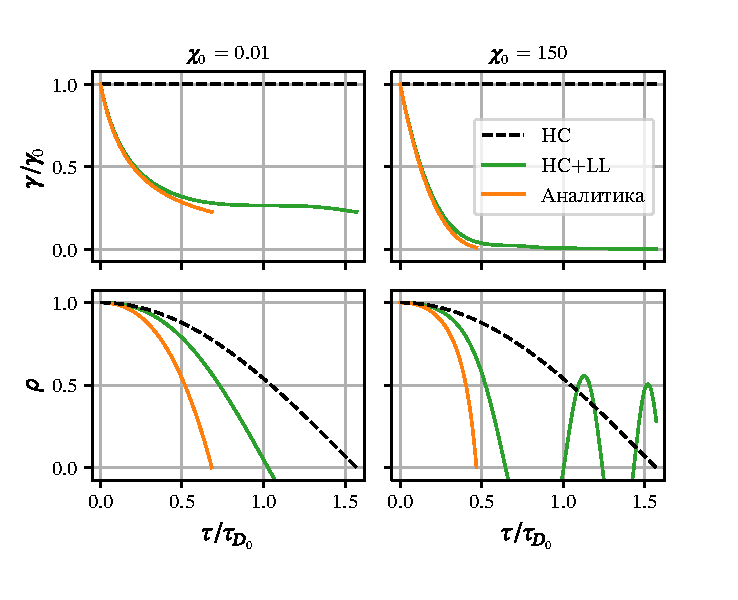
\includegraphics{beam-motionless.pdf}}
    \caption[Сравнение аналитического и численного решений уравнений движения частиц при столкновении пучков в режиме преобладания излучения]{\label{fig:ch3/sec2/motionless} 
    Сравнение приближённого решения~\eqref{eq:ch3/gamma_const}--\eqref{eq:ch3/rho_const} (оранжевая линия) с численным решением уравнений~\eqref{eq:ch3/dydt}--\eqref{eq:ch3/dgdt} (зелёная линия) при $\varkappa_0=5$. Для левой колонки $\chi_0=0.01$, для правой~---~$\chi_0=150$. Чёрная штриховая линия соответствует решению уравнения~\eqref{eq:ch3/dydt} с постоянной энергией частицы $\gamma$.}
\end{figure}

\paragraph{Поправки модели}

Точность аналитической модели можно значительно повысить за счет двух изменений.
Во-первых, будем использовать среднюю поперечную координату в правой части уравнения~\eqref{eq:ch3/dydt} вместо ее начального значения $\rho_0$,
\begin{align}
    &\frac{d^2\rho}{d\tau^2} = -\frac{\mu}{\gamma} , \\
    \label{rho2}
    &\frac{d\gamma}{d\tau} = -P \left( \mu \chi_0 \frac{\gamma}{\gamma_0} \right), \\
    &\mu \equiv \frac{1}{\tau_D} \int^{\tau_D}_{0} \rho \left( \tau' \right) \dd \tau' < 1. 
\end{align}
Во-вторых, <<сошьём>> решения в КЭД и классическом режимах в момент времени $\tau_1$, при котором параметр частицы $\chi$ достигает некоторого порогового значения $\chi_1 \sim 1$, если его начальное значение было достаточно велико, то есть $\chi_0 > \chi_1$.
Тогда при $\tau < \tau_1$ уравнения движения имеют следующее решение
\begin{align}
    \label{eq:ch3/gamma_Q}
    &\gamma_Q(\tau) = \gamma_0 \left(1 - \tilde\varkappa_0 \frac{\tau}{\tau_{D_0}} \right)^{3} ,\\
    \label{eq:ch3/rho_Q}
    &\rho_Q(\tau) = 1 - \frac{\tau^2}{\tau_{D_0}^2}\left( 1-\tilde\varkappa_0 \frac{\tau}{\tau_{D_0}} \right)^{-1}, \\
    &\tilde\varkappa_0 = \sqrt{\frac{2}{9\gamma_0\mu}}P_Q(\mu\chi_0).
\end{align}
Отметим, что переменная $\tilde\varkappa_0$ (а также $\tilde\varkappa_1$ ниже) включает дополнительный множитель $1/3$ по сравнению с определением $\varkappa$ в уравнении~\eqref{eq:ch3/condition}, что несколько сокращает последующие выражения.
Момент времени $\tau_1$ находится из условия
\begin{align}
    \label{eq:ch3/chi1}
    \chi = \chi_0 \frac{\gamma_Q(\tau_1) \rho_Q(\tau_1)}{\gamma_0 } \equiv \chi_0 \frac{\gamma_1 \rho_1}{\gamma_0 } = \chi_1.
\end{align}
Для нахождения приближённого решения этого уравнения рассмотрим следующее вспомогательное уравнение относительно $x$
\begin{equation}
    \label{app.zeta}
    k_1 = \left( 1 - \frac{x^2}{1 - k_2 x} \right) \left( 1 - k_2 x \right)^3 .
\end{equation}
Поскольку оба множителя в правой части убывают с ростом $x$, очевидно, что $x < x_{1,2}$, где $x_{1,2}$ удовлетворяют следующим уравнениям
\begin{align}
    &k_1 = {\left(1 - k_2 x_1\right)}^3 ,\\
    &k_1 = 1 - \frac{x_2^2}{1 - k_2 x_2}.
\end{align}
Эти уравнения имеют следующие решения
\begin{align}
    &x_1 = \frac{1-\sqrt[3]{k_1}}{k_2}, \\
    &x_2 = \frac{k_2(1-k_1)}{2} \left( \sqrt{1 + \frac{4}{k_2^2 (1-k_1)}} - 1 \right).
\end{align}
Таким образом, приближенное решение уравнения ~\eqref{app.zeta} может быть найдено как $x = \text{min}\{x_1, x_2\}$.
Наконец $\tau_1$ находится путём выполнения замены
\begin{equation}
    x \rightarrow \frac{\tau_1}{\tau_{D_0}} ,\ 
    k_1 \rightarrow \frac{\chi_1}{\chi_0} = \zeta ,\ 
    k_2 \rightarrow \tilde{\varkappa}_0.
\end{equation}
Из уравнения~\eqref{eq:ch3/chi1} отношение $\gamma_1/\gamma_0$ можно найти следующим образом
\begin{equation}
    \frac{\gamma_1}{\gamma_0} = \frac{\chi_1}{\chi_0} \frac{1}{\rho_1} \equiv \frac{\zeta}{\rho_1},
\end{equation}
где мы ввели $\zeta=\chi_1/\chi_0$.

\begin{figure}
    \centerfloat{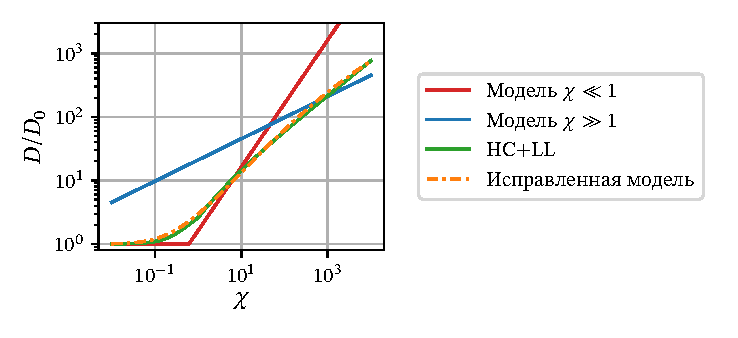
\includegraphics{beam-scalings.pdf}}
    \caption[Сравнение точности вычисления отношения $D/D_0$ в помощью различных методов]{\label{fig:ch3/scalings} 
    Сравнение отношения $D/D_0$, рассчитанного с помощью предельного выражения~\eqref{eq:ch3/dratio_simple} (красная линия соответствует классическому пределу, синяя~---~квантовому), с помощью исправленной модели (оранжевая штрих-пунктирная линия) и с помощью численного решения уравнений движения~\eqref{eq:ch3/dydt}--\eqref{eq:ch3/dgdt} (зелёная линия), как функция $\chi$ при фиксированном значении $r_\mathrm{b} = \SI{10}{\um}$.}
\end{figure}

При $\tau > \tau_1$ по определению необходимо использовать классические формулы для мощности излучения, так что решение уравнений движения имеет вид
\begin{gather}
    \label{eq:ch3/gamma_C}
    \gamma_C(\tau) = \gamma_1 \left(1+ 3\tilde\varkappa_1\frac{\tau - \tau_1}{\tau_{D_1}} \right)^{-1} ,\\
    \label{eq:ch3/rho_C}
    \rho_C(\tau) = \rho_1 + \dot{\rho}_1 \frac{\tau - \tau_1}{\tau_{D_1}} - \frac{(\tau-\tau_1)^2}{\tau_{D_1}^2}\left(1+\tilde\varkappa_1\frac{\tau - \tau_1 }{\tau_{D_1}}\right), 
\end{gather}
где
\begin{gather}
    \tau_{D_1}  = \sqrt{2 \gamma_1}, \\
    \tilde\varkappa_1 = \sqrt{\frac{2}{9\gamma_1\mu}}P_C(\mu\chi_1) , \\
    \dot{\rho}_1 = \tau_{D_1} \dot{\rho}_Q (\tau = \tau_1) = - \sqrt{\frac{\zeta}{\rho_1}}\frac{\tau_1 }{\tau_{D_0}}\frac{2-\tilde\varkappa_0 \frac{\tau_1}{\tau_{D_0}}}{\left( 1 - \tilde\varkappa_0 \frac{\tau_1}{\tau_{D_0}} \right)^2}. 
\end{gather}
Время фокусировки можно вычислить из уравнения $\rho_C(\tau_D) = 0$, имеющее явное, однако слишком громоздкое решение.
Найдём приближенное решение этого уравнения.
Для этого рассмотрим следующее вспомогательное уравнение относительно $x$
\begin{equation}
    \label{app.rho}
    0 = k_1 + k_2 x - x^2 \left( 1 + k_3 x \right).
\end{equation}
При больших значениях $k_3$ решения этого уравнения можно грубо оценить следующим образом
\begin{equation}
    x_1 = \sqrt[3]{\frac{k_1}{k_3}}.
\end{equation}
Для меньших значений $k_3$ мы можем сначала найти решение, положив $k_3=0$, т.е.
\begin{equation}
    0 = k_1 + k_2 x' - x'^2.
\end{equation}
Приведенное выше уравнение имеет решение
\begin{equation}
    x' = \frac{k_2}{2} + \sqrt{k_1 + \frac{k_2^2}{4}} .
\end{equation}
Предполагая, что решение уравнения ~\eqref{app.rho} лишь немного отличается от $x'$, т. е. $x=x'+x''$, мы можем разложить это уравнение по $x''$ и оставить только линейные члены:
\begin{equation}
    k_2 x'' + 2 x'' x' (1 + k_3 x') - k_3 x'^3 = 0.
\end{equation}
Отсюда получаем, что $x$ можно приближённо вычислить следующим образом
\begin{equation}
    x_2 = x' - \frac{k_3 x'^3}{k_2 + 2 x' (1 + k_3 x')}.
\end{equation}
Наконец, выбирается наименьшее из $x_{1,2}$, т.е.~$x~=~\text{min}\{x_1, x_2\}$.
Чтобы найти $\tau_2$, выполним следующую замену
\begin{equation}
    x \rightarrow \frac{\tau_2}{\tau_{D_1}} ,\ 
    k_1 \rightarrow \rho_1 ,\ 
    k_2 \rightarrow \dot{\rho}_1 ,\ 
    k_3 \rightarrow \tilde{\varkappa}_1. 
\end{equation}
Таким образом, 
\begin{gather}
    \label{eq:ch3/est0}
    \frac{\tau_D}{\tau_{D_0}} = \tau_1 + \tau_2 \sqrt{\frac{\zeta}{\rho_1}} ,\\
    \label{eq:ch3/est1}
    \tau_1 = \text{min}\left \{ \frac{1 - \zeta ^{1/3}}{\tilde\varkappa_0} \frac{\tilde\varkappa_0 \left( 1 - \zeta \right)}{2}  \left( \sqrt{1 + \frac{4}{\tilde\varkappa_0^2 \left( 1 - \zeta \right)}} - 1 \right) \right \}, \\
    \label{eq:ch3/est2}
    \tau_2 = \text{min}\left\{ \sqrt[3]{\frac{\rho_1}{\tilde\varkappa_1}}, \tau' - \frac{\tilde\varkappa_1 \tau'^3}{\dot\rho_1 + 2\tau' \left( 1 + \tilde\varkappa_1 \tau' \right)} \right\} ,\\
    \tau' = \sqrt{\rho_1 + \frac{\dot\rho_1^2}{4}} - \frac{\dot\rho_1}{2}.
\end{gather}
В случае $\chi_0 < \chi_1$, $\tau_1 \equiv 0$ и $\chi_1$ необходимо заменить на $\chi_0$ в $\tau_2$.

По аналогии с уравнением~\eqref{eq:ch3/beta0} параметр, определяющий значимость излучения, может быть выражен следующим образом
\begin{equation}
    \tilde\varkappa = \alpha \sqrt{ \frac{2}{9} r_\mathrm{b} a_\mathrm{S}} \times
    \begin{dcases}
        {\left( \mu\chi_0 \right)}^{2/3} ,\; \chi_0 < \chi_1, \\
        {\left( \mu\chi_0 \right)}^{1/6} ,\; \chi_0 > \chi_1,
    \end{dcases}
\end{equation}
и несложно показать, что $\tilde\varkappa_1$ можно выразить через $\tilde\varkappa$.
Таким образом, параметр разрушения с учётом реакции излучения в скорректированной модели равен
\begin{equation}
    D = {D_0} \left(\frac{\tau_{D_0}}{\tau_D}\right)^2.
\end{equation}
Рисунок~\ref{fig:ch3/scalings} показывает, что расчет параметра разрушения с использованием этой скорректированной модели значительно превосходит использование простых предельных выражений~\eqref{eq:ch3/dratio_simple}.
Заметим, что хотя $\mu$ следует вычислять самосогласованным образом из полученного выше решения, численный анализ показывает, что значение $\mu$ близко к $0.5$.
Таким образом, чтобы найти аналитическое решение, мы рассматриваем $\mu$ как свободный параметр, который мы устанавливаем равным $0.5$.
Это также подтверждается тем, что варьирование $\mu$ в диапазоне 0.3--0.7 не приводит к существенному изменению конечного значения параметра разрушения.
Согласно уравнениям~\eqref{eq:ch3/est1}--\eqref{eq:ch3/est2}, отношение $D/D_0$ может быть выражено как функция только от двух начальных параметров: радиуса пучка $r_\mathrm{b}$ и значения $\chi_0$.
Данный факт позволяет провести за разумное время сканирование по параметрам с помощью полноразмерного трёхмерного QED-PIC моделирования и вычислить значение $D/D_0$, основываясь на результатах такого моделирования (см. п.~\ref{sec:ch3/sec/PIC}).

\subsection{Взаимодействие длинных пучков}
\label{sub:ch3/sec3/Long}

В данном разделе обсуждается взаимодействие длинных однородных пучков противоположно заряженных частиц, когда число бетатронных колебаний велико $\sigma_z / (c \tau_{D_0}) \gg 1$ и радиационные потери на излучение незначительны в течение одного периода, что соответствует пределу $\varkappa \ll 1$.
Такая конфигурация может соответствовать взаимодействию пучков с существенно различающимися плотностями энергии в системе центра масс, что может возникать из-за большей массы, Лоренц-фактора или плотности частиц одного пучка по сравнению с другим в лабораторной системе отсчета.
Характерным примером такого сценария является столкновении электронного и протонного пучков.
В таком случае характерный временной масштаб эволюции более энергичного пучка намного больше, чем у встречного, поэтому все частицы встречного пучка ощущают практически невозмущенное поле в отличие от случая, рассмотренного в предыдущем разделе, когда данное утверждение верно только для частиц на фронте пучка.
Для простоты рассмотрим взаимодействие однородных пучков $\eta_z =\eta_r =\eta = 1$, для которых $\mathcal{E}(\rho) = \rho$.
Удобно ввести следующие переменные
\begin{gather}
    \label{b}
    a^{2} = \rho^{2}+\gamma\left(\dv{\rho}{\tau}\right)^2,\\
    \varphi = \arctan(\dv{\rho}{\tau}\frac{\sqrt{\gamma}}{\rho}) ,
\end{gather}
где $a$ и $\varphi$~---~амплитуда и фаза бетатронных колебаний ($\rho = a \cos\varphi $).
В новых переменных уравнение~\eqref{eq:ch3/app_g} принимает вид
\begin{equation}
    \label{rho}
    \dv{a}{\tau} = -\frac{a}{2\gamma}\sin^{2}\varphi\;P\left( \frac{\chi_0}{\gamma_0} a \gamma  |{\cos\varphi} | \right).
\end{equation}
Чтобы вычислить медленно меняющуюся амплитуду бетатронных колебаний, $A = \left\langle a\right\rangle $, усредним уравнение~\eqref{rho} по $\varphi$ и пренебрежём быстрыми составляющими амплитуды $a$ и энергии $\gamma$
\begin{gather}
    \label{dst-2}
    \dv{A}{\tau} = -\frac{A}{2\overline{\gamma}}f_{1}\left(\frac{\chi_0}{\gamma_0} A \overline{\gamma} \right),\\
    \dv{\overline{\gamma}}{\tau} = -f_{2}\left(\frac{\chi_0}{\gamma_0} A \overline{\gamma} \right),\\
\end{gather}
где 
\begin{gather}
    \label{f1}
    f_{1}(v) = \frac{1}{2\pi}\intop_{0}^{2\pi}\sin^{2}\varphi\;P\left(v|{\cos\varphi} |\right)\dd\varphi ,\\
    f_{2}(v) = \frac{1}{2\pi}\intop_{0}^{2\pi}P\left(v |{\cos\varphi}|\right)\dd\varphi ,
\end{gather}
и $\overline{\gamma} = \langle\gamma\rangle$.
Вводя $\overline{\chi}=\left\langle \chi\right\rangle = \chi_0 A \overline{\gamma} / \gamma_0$, получаем систему, описывающую усредненную по бетатронным колебаниям динамику электрона
\begin{gather}
    \label{v}
    \frac{d\overline{\chi}}{d\tau} = -\frac{\overline{\chi}}{2\overline{\gamma}}\left[f_{1}\left(\overline{\chi}\right)+2f_{2}\left(\overline{\chi} \right)\right],\\
    \label{gf2}
    \frac{d\overline{\gamma}}{d\tau} = -f_{2}\left(\overline{\chi } \right).
\end{gather}
Данная система имеет следующий интеграл движения
\begin{gather}
    \ln \overline{\gamma} - g (\overline{\chi} )  = \mathrm{const} \label{integral} , \\
    g (v) = \int \frac{2f_{2}(v)\dd v} {v f_{1}\left(v \right)+2 v f_{2}\left(v \right)}.
\end{gather}
\begin{figure}[ht]
	\centerfloat{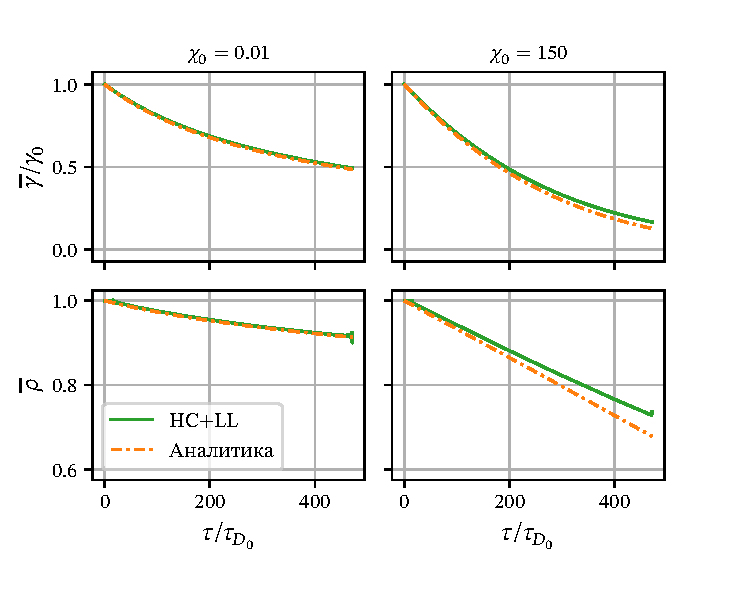
\includegraphics{beam-long.pdf}}
	\caption[Сравнение аналитического и численного решений уравнений движения частиц при столкновении длинных пучков в режиме слабого пучкового излучения]{\label{fig:ch3/sec3/long} 
    Сравнение аналитического решения~\eqref{eq:ch3/long_gC}--\eqref{eq:ch3/long_rC} и~\eqref{eq:ch3/long_gQ}--\eqref{eq:ch3/long_rQ} (оранжевая штрих-пунктирная линия) и численного решения уравнений~\eqref{eq:ch3/dydt}--\eqref{eq:ch3/dgdt} (зелёная линия) при $\varkappa_0=0.005$. В левой колонке $\chi_0=0.01$, в правой~---~$\chi_0=150$.}
	\label{long}
\end{figure}
В классическом пределе ($\chi \ll 1$) $f_{2}(v) = 4 f_{1}(v)=P_C(v)/2$ и интеграл движения принимает вид
\begin{equation}
    \overline{\gamma}^{-9/8} \overline{\chi} = \text{const}.\label{integral1}
\end{equation}
Из уравнений~\eqref{gf2} и \eqref{integral1} следует, что
\begin{gather}
    \label{eq:ch3/long_gC}
    \overline{\gamma} = \gamma_{0} S(\tau)^{-4/5} ,\\
    \label{eq:ch3/long_rC}
    \overline \rho = \rho_{0} S(\tau)^{-1/10},\\
    % & \overline{\chi} = \chi_{0} S(\tau)^{-9/10}, \\
    S(\tau) = 1+\frac{5}{8}\left( \varkappa\frac{\tau}{\tau_{D_0}} \right).
\end{gather}
% Fig.~\ref{long1} demonstrates numerical solution of Eqs.~\eqref{eq:ch3/y2}-\eqref{eq:ch3/c2}
% and analytical result  given by Eq.~\eqref{eq:ch3/long_gC} for $\ln\gamma(t)$ which are in a good agreement.
В существенно квантовом пределе (${\chi\gg1}$)
\begin{equation}
    f_{2}(v)= (8/3) f_1 (v) = \Gamma(5/6) \Gamma^{-1}(4 /3) \pi^{-1/2} P_Q(v),
\end{equation} 
и интеграл движения принимает вид
\begin{equation}
    \overline{\gamma}^{-19/16}\overline{\chi} = \text{const}.\label{integral1-1}
\end{equation}
Уравнения~\eqref{gf2} и \eqref{integral1-1} имеют следующие решения
\begin{gather}
    \label{eq:ch3/long_gQ}
    \overline{\gamma} = \gamma_{0} S(\tau)^{24/5},\\
    \label{eq:ch3/long_rQ}
    \overline\rho  = \rho_{0} S(\tau)^{9/5},\\
    % &\overline{\chi} = \chi_{0} S(\tau)^{57/10}, \\
    S(\tau) = 1-\frac{5}{24\sqrt\pi}\frac{\Gamma(5/6)}{\Gamma(4/3)}\left( \varkappa\frac{\tau}{\tau_{D_0}} \right) \approx 1 - 0.149\left( \varkappa\frac{\tau}{\tau_{D_0}} \right).
\end{gather}
Рисунок~\ref{fig:ch3/sec3/long} демонстрирует хорошее совпадение численного решения уравнений~\eqref{eq:ch3/dydt}--\eqref{eq:ch3/c2} и аналитического решения~\eqref{eq:ch3/long_gC} и~\eqref{eq:ch3/long_gQ}.

\subsection{QED-PIC моделирование}
\label{sec:ch3/sec/PIC}

Для подтверждения предсказаний модели, разработанной в п.~\ref{sub:ch3/sec3/Model} было выполнено полноразмерное трехмерное QED-PIC моделирование с использованием кода QUILL~\cite{QUILL}, который позволяет моделировать КЭД процессы с учётом их стохастичности с помощью метода Монте-Карло.
Принимая $z$ за ось распространения пучка, параметры моделирования составляли $\Delta t = 0,6 \Delta z$, $\Delta x = \Delta y = 2,5 \Delta z = r_\mathrm{b} / 20$.
Для всех проведенных моделирований шаг по времени $\Delta t$ был намного меньше, чем средняя задержка между последовательными КЭД процессами (излучением гамма-кванта или рождения электрон-позитронной пары).
Для численного решения уравнений Максвелла использовалась гибридная схема FDTD, подробно опиаснная в разделе~\ref{sub:ch3/sec4/Hybrid}, а для решения уравнений движения частиц использовался пушер Вэя~\cite{Vay08}.
Моделирование также выполнялось с использованием кода VLPL~\cite{pukhov1999three,NDFX,PhysRevE_94_063204} в сочетании с бездисперсионной схемой решения уравнений Максвелла~---~RIP~\cite{Pukhov2019}.
Различия между результатами моделирования с использованием двух разных кодов были незначительными.
На рисунке~\ref{fig:ch3/densities}, демонстрирующем пример результатов моделирования, видно, что при $\chi_0 = 10$ происходит обильное рождение вторичных электронов и позитронов.
Поскольку этот процесс не влияет на движение частиц пучка на фронте, формирование и развитие такого каскада подробно не обсуждается.
Также отметим развитие поперечной шланговой неустойчивости в моделировании с учетом КЭД процессов, которая будет описана ниже.

\begin{figure}[ht]
    \centerfloat{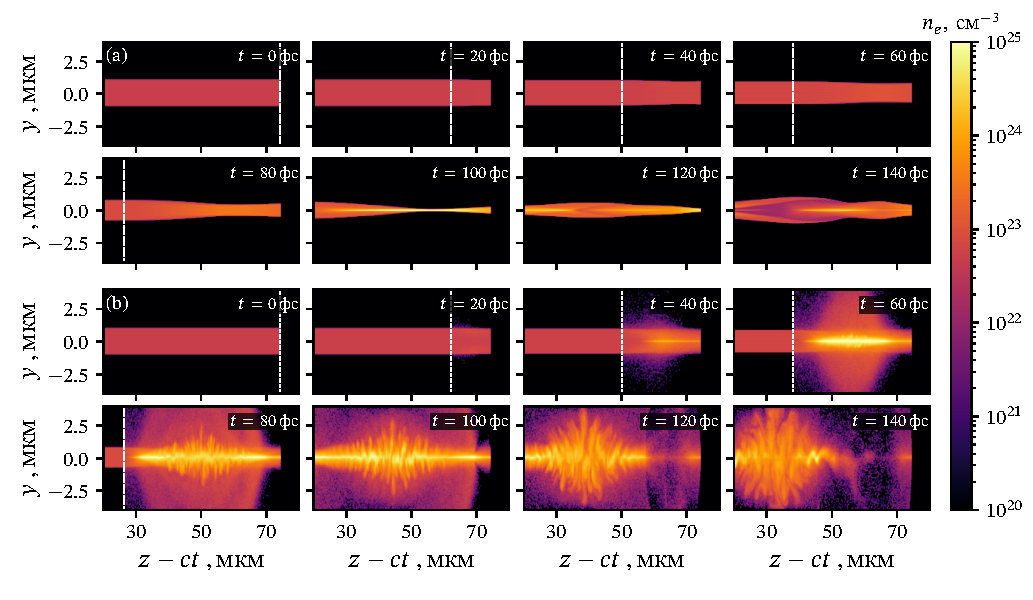
\includegraphics{beam-density.pdf}}
    \caption[Распределение плотности электронов в различные моменты времени в PIC моделировании столкновения электронного и позитронного пучков]{\label{fig:ch3/densities} 
    Распределение плотности электронов в различные моменты времени в PIC моделировании с параметрами $r = \SI{1}{\um}$, $\chi = 10$. 
    Белая штриховая линия соответствует положению фронта встречного позитронного пучка.
    Представлены результаты моделирования (a) без учёта и (b) с учётом КЭД процессов.}
\end{figure}

Мы провели серию моделирований с различными значениями начального радиуса пучков $r_\mathrm{b}$ и величины $\chi_0$.
Длина пучка выбиралась таким образом, чтобы для каждого моделирования параметр разрушения без учёта реакции излучения, т.е. $D_0$, равнялся 10.
Это было сделано для того, чтобы иметь четкий способ определения времени фокусировки, используемого при расчете параметра разрушения.
В этом отношении наше QED-PIC моделирование не соответствует какому-либо конкретному эксперименту, возможному, например, на установке FACET-II, поскольку последний требует очень короткого времени взаимодействия для подавления радиационных потерь~\cite{yakimenko2019prospect}.
Вместо этого QED-PIC моделирование использовалось как средство для решения уравнений движения частиц в самосогласованно вычисляемом электромагнитном поле и с учетом стохастического характера КЭД процессов.
Для каждого моделирования мы отслеживали несколько сотен частиц, расположенных на фронте и периферии электронного пучка, по траекториям которых рассчитывалось среднее время пересечения оси пучка.
Примеры таких траекторий, численное решение уравнений~\eqref{eq:ch3/dydt}--\eqref{eq:ch3/dgdt} и приближенное аналитическое решение показаны на Рис.~\ref{fig:ch3/tracks}.
Для каждой пары значений $r_\mathrm{b}$ и $\chi_0$ проводилось два моделирования: с учётом и без КЭД процессов.
Сравнивая среднее время фокусировки в этих двух моделированиях, рассчитывалось отношение $D/D_0$ в широком диапазоне начальных параметров, что представлено на Рис.~\ref{fig:ch3/disruption} вместе с оценкой из уравнений~\eqref{eq:ch3/est0}-- \eqref{eq:ch3/est2} (в котором были использованы свободные параметры $\mu=0.5$, $\chi_1=1$) и результатом численного решения одночастичных уравнений движения~\eqref{eq:ch3/dydt}- -\eqref{eq:ch3/dgdt}.

\begin{figure}[ht]
    \centerfloat{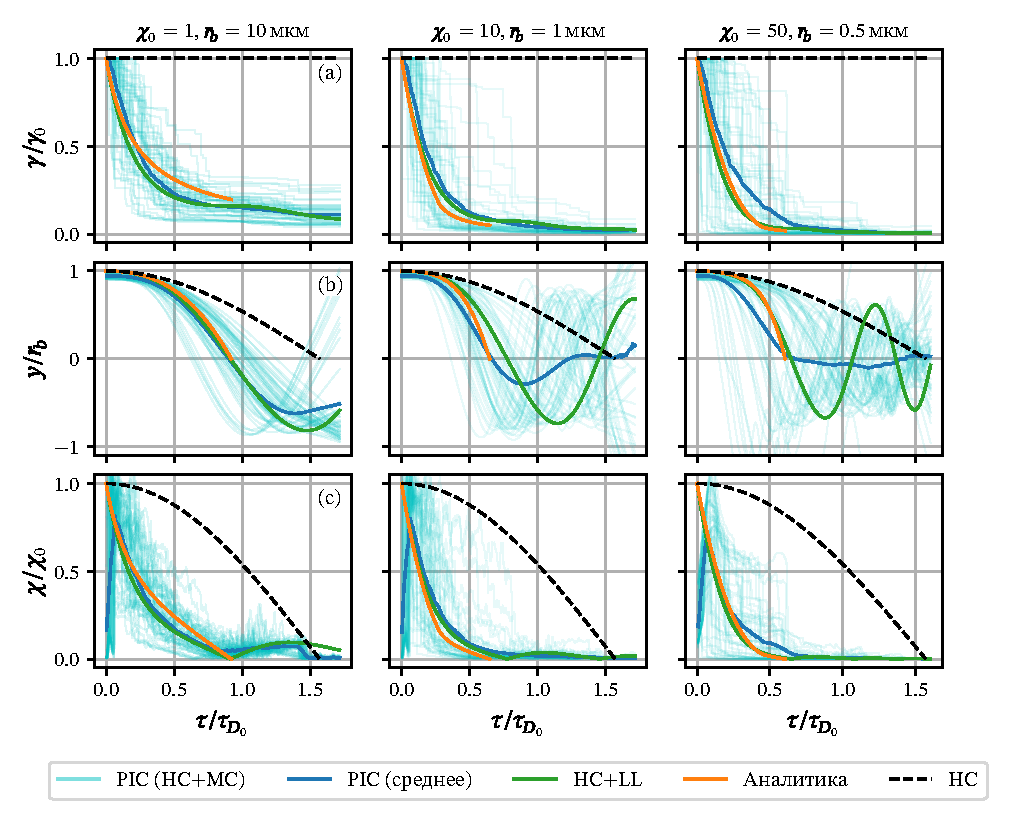
\includegraphics{beam-tracks.pdf}}
    \caption[Динамика электронов в поле встречного позитронного пучка]{\label{fig:ch3/tracks} 
    Динамика электронов в поле встречного позитронного пучка. (a) Энергия электронов, (b) смещение относительно оси пучка и (c) величина параметра $\chi$ как функции времени.
    Тонкие голубые линии соответствуют траекториям отдельных частиц в QED-PIC моделировании, сплошная синяя линия~---~величинам, усреднённым по этим частицам, зелёная линия~---~численному решению уравнений~\eqref{eq:ch3/dydt}--\eqref{eq:ch3/dgdt}, оранжевая линия~---~аналитическому решению ~\eqref{eq:ch3/gamma_Q}--\eqref{eq:ch3/rho_Q},~\eqref{eq:ch3/gamma_C}--\eqref{eq:ch3/rho_C}, чёрная штриховая линия~---~решению уравнения~\eqref{eq:ch3/dydt} без учёта пучкового излучения, т.е. с постоянной энергией $\gamma$.
    Различные колонки соответствуют различным начальным параметрам $r_\mathrm{b}$ и $\chi_0$.}
\end{figure}

\begin{figure}[ht]
    \centerfloat{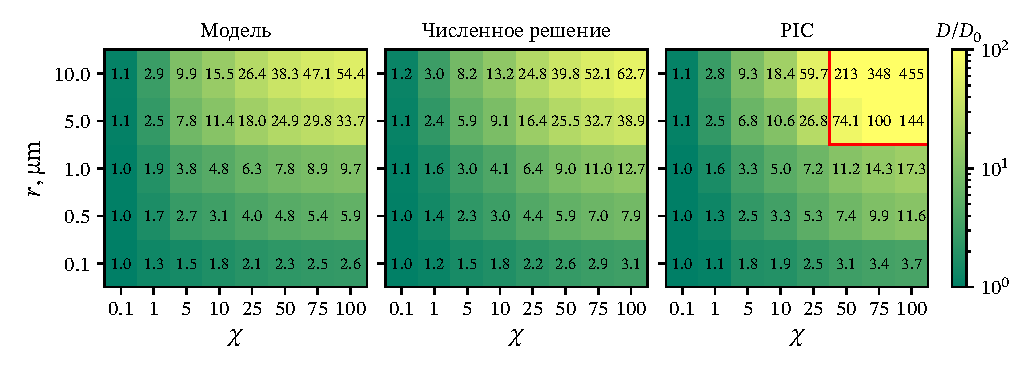
\includegraphics{beam-map.pdf}}
    \caption[Сравнение отношения параметра разрушения с учётом реакции излучения к таковому без учёта реакции излучения, рассчитанного различными способами]{\label{fig:ch3/disruption} 
    Отношение $D/ D_0$, рассчитанное (левая колонка) по аналитическому решению~\eqref{eq:ch3/est0}--\eqref{eq:ch3/est1}, (средняя колонка) по численному решению уравнений~\eqref{eq:ch3/dydt}--\eqref{eq:ch3/dgdt}, (правая колонка) полученная по результатам QED-PIC моделирования.
    Красная рамка обозначает область, в которой был использован альтернативный критерий разрушения (см. текст).}
\end{figure}

Важно отметить, что для больших значений $r_\mathrm{b}$ и $\chi_0$ (область, отмеченная красной рамкой на Рис.~\ref{fig:ch3/disruption}) для расчета параметра разрушения был использован альтернативный критерий.
Это связано с тем, что при таких параметрах потери энергии из-за излучения настолько велики, что через некоторое время частицы пучка перестают быть релятивистскими, а их продольная скорость становится сравнимой с их поперечной скоростью, так что в конце концов частицы прекращают свое направленное движение и начинают вращение, не пересекая ось луча (\fixme{рисунок с треками}).
В таких случаях для вычисления параметра разрушения вместо времени достижения частицей оси пучка, использовалось время, за которое продольная скорость частицы достигала значения $0.5c$.
Поскольку наша аналитическая модель предполагает, что продольная скорость всегда больше поперечной, она не может быть применена в этих случаях.
% Изучение столкновений пучков в этой области параметров требует отдельного специального исследования.
Как было указано выше, наша аналитическая модель предсказывает, что отношение $D/D_0$ не зависит явно от энергии частиц.
Для подтверждения этого нами было выполнено несколько QED-PIC моделирований с разными начальными энергиями частиц, но с одинаковыми значениями $\chi_0$ и $r_\mathrm{b}$.
Результаты моделирования показывают, что до тех пор, пока энергия частицы достаточно велика, для того чтобы частицы оставались ультрарелятивистскими до достижения оси пучка, результирующее отношение $D/D_0$ не зависит от энергии частицы.

\fixme{Мы не проводили QED-PIC-симуляции взаимодействия пучков в режиме, когда лучевое излучение требует много бетатронных колебаний для значительного уменьшения энергии частиц ($\varkappa \ll 1$) по нескольким причинам.
Во-первых, такие симуляции заняли бы значительно больше времени.
А во-вторых, поскольку этот режим в большей степени связан с взаимодействием пучков с существенно различающимися плотностями энергии (в системе центра масс), при котором более энергичный из них сильно не деформируется, такое взаимодействие может быть достаточно смоделировано одной частицей динамики в невозмущенном поле медленно эволюционирующего (энергетического) сгустка, что было сделано в разд.~\ref{sub:ch3/sec3/Model}.}

\subsection{Обсуждение}
\label{sec:ch3/sec/Discussion}

Схема, обсуждаемая в публикации~\cite{yakimenko2019prospect}, для наблюдения эффектов непертурбативной КЭД с помощью лобового столкновения электронного и позитронного пучков, требует столкновения пучков очень малому параметру разрушения.
Это требование накладывает жесткие ограничения на длину и диаметр пучка.
Однако, как показано выше на параметр разрушения также влияет реакция излучения, которая не учитывается при стандартном способе расчёта параметра разрушения.
Наша аналитическая модель показывает, что при параметрах пучка, необходимых для достижения значения $\chi \sim 1600$ при энергии пучка $\SI{125}{\giga\electronvolt}$, полном заряде $\SI{3}{\nano\coulomb}$ и радиусе $\SI{10}{\nano\meter}$, увеличение разрушения из-за излучения достигает 60\%.
Для будущих коллайдеров CLIC и ILC, наоборот, реакция излучения может несколько смягчить требования к параметрам пучка для достижения желаемой яркости в области взаимодействия, что частично достигается за счет использования плоских пучков.
Хотя при выводе аналитической оценки отношения $D/D_0$ мы рассматривали цилиндрические пучки, полученные результаты можно применить к конфигурациям плоских пучков, предлагаемых для использования на установках CLIC и ILC.
Для частиц, с начальным отклонением, лежащим на одной из осей пучка, движение остается плоским, и поэтому уравнения ~\eqref{eq:ch3/dydt}--\eqref{eq:ch3/dgdt} остаются справедливыми.
Таким образом, вычисляя значения $\chi_0$ и $r_\mathrm{b}$ относительно распределения заряда пучка (см., например,~\cite{bassetti1983properties} для распределения электромагнитных полей для эллиптического гауссова распределения заряда), параметр разрушения может быть вычислен для конкретной оси с использованием нашей аналитической модели.
Выполнение этой процедуры, приводит к заключению, что для ожидаемых параметров пучка на установке CLIC увеличение параметра разрушения составляет примерно $35\%$ для более длинной оси и только на $5\%$ для более короткой.
Для круглого пучка с тем же полным зарядом и площадью поперечного сечения увеличение параметра разрушения составляет около $35\%$ по обеим осям, что  подтверждает тот факт, что использование плоских пучков снижает влияние реакции излучения на столкновение пучков.
Для параметров, ожидаемых на установке ILC, увеличение разрушения не превышает $5\%$ по обеим осям из-за достаточно низкого значения $\chi$.

\begin{figure}[ht]
    \centerfloat{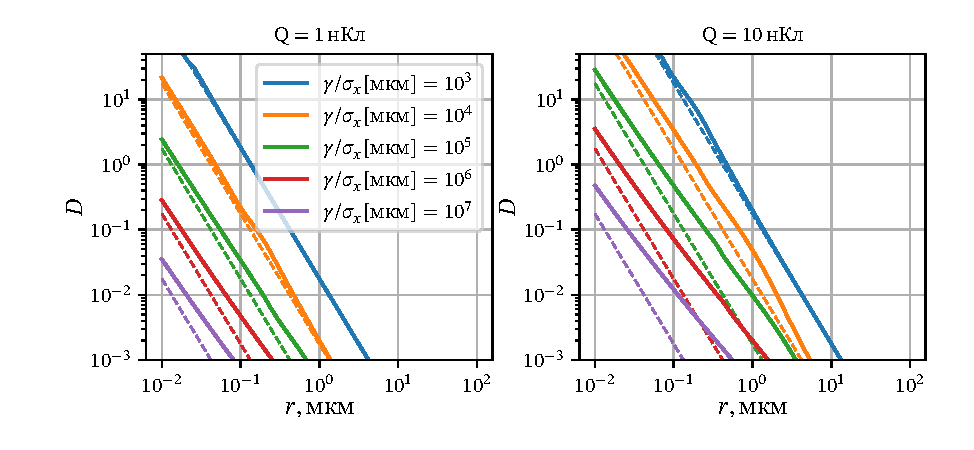
\includegraphics{beam-Q_disruption.pdf}}
    \caption[Параметр разрушения, рассчитанный с учётом и без учёта пучкового излучения, для различных параметров пучка]{\label{fig:ch3/Q_disruption} 
    Параметр разрушения, рассчитанный с учётом (сплошные линии) и без учёта (штриховые линии) пучкового излучения, для различных параметров пучка.}
\end{figure}

На Рис.~\ref{fig:ch3/Q_disruption} показано, как реакция излучения влияет на разрушение пучков при различных параметрах.
В частности, показано, что столкновение пучков с достаточно большим полным зарядом ($> \SI{10}{\nano\coulomb}$ 10 нКл) и малыми радиусами может быть подвержено существенному влиянию пучкового излучения.
Другая интересная зависимость заключается в том, что хотя увеличение энергии частиц и/или уменьшение длины пучка (при сохранении того же общего заряда) уменьшает параметр разрушения, оно в то же время приводит к увеличению значимости пучкового излучения.
Таким образом, отношение $D/D_0$ можно использовать для определения того, является ли излучение при столкновении пучков значительными или нет.

\begin{comment}
    Динамика пучка при взаимодействии пучков с противоположными зарядами была исследована в режиме доминирования излучения.
    Оказывается, радиус пучка $r_\mathrm{b}$ и $\chi_0$ являются ключевыми параметрами, определяющими усиление фокусировки или разрушения пучков.
    Для однородного пучка параметр $\chi_0$ можно рассчитать по плотности пучка $n_e$ или полному заряду пучка $Q$ следующим образом
    \begin{equation}
        \chi_0 \approx 5.3\; \frac{\varepsilon_\mathrm{b}[100\,\text{GeV}]\ Q[\text{nC}]}{r_\mathrm{b}[\upmu \text{m}]\; \sigma_z [\upmu \text{m}]} 
            \approx  2.67\; \varepsilon_\mathrm{b}[100\,\text{GeV}]\; n_e[10^{21}\text{cm}^{-3}] \;r_\mathrm{b}[\upmu \text{m}],
    \end{equation}
    где $\varepsilon_\mathrm{b}$~---~энергия частиц пучка.
    Согласно нашей модели постоянной силы отношение параметра разрушения с учётом пучкового излучения к параметру разрушения без его учёта также может быть выражено через параметры пучка.
    В классическом режиме ($\chi_0 \ll 1$)
    \begin{equation}
        \begin{aligned}
            D &\approx 4\times 10^{-3} \frac{Q[\text{nC}]^2}{r_\mathrm{b}[\upmu \text{m}]^{8/3}} 
            &\approx 8\times 10^{-4} n_e[10^{21}\text{cm}^{-3}]^2\sigma_z [\upmu \text{m}]^2 r_\mathrm{b}[\upmu \text{m}]^{2/3},
        \end{aligned}
    \end{equation}
    \begin{equation}
        \begin{aligned}
            \frac{D}{D_0} &\approx  22.1\; \frac{\varepsilon_\mathrm{b} [100\,\text{GeV}]\; Q[\text{nC}]}{r_\mathrm{b}[\upmu \text{m}]^{2/3} \;\sigma_z [\upmu \text{m}]} \\
            &\approx 8.9\; \varepsilon_\mathrm{b} [100\,\text{GeV}] \;n_e[10^{21}\text{cm}^{-3}] \;r_\mathrm{b}[\upmu \text{m}]^{2/3},
        \end{aligned}
    \end{equation}
    и в квантовом режиме ($\chi_0 \gg 1$)
    \begin{equation}
        \begin{aligned}
            D &\approx 7.2\times 10^{-3}\left( \frac{Q[\text{nC}]^2 \sigma_z[\upmu \text{m}]}{\varepsilon_\mathrm{b}[100\,\text{GeV}] r_\mathrm{b}[\upmu \text{m}]^2} \right)^{2/3}    \\
            &\approx 1.4\times 10^{-3}\left( \frac{n_e[10^{21}\text{cm}^{-3}]^{2} \sigma_z[\upmu \text{m}]^3 }{\varepsilon_\mathrm{b} [100\,\text{GeV}] r_\mathrm{b}[\upmu \text{m}]^{-2}} \right)^{2/3} ,
        \end{aligned}
    \end{equation}
    \begin{equation}
        \begin{aligned}
            &\frac{D}{D_0} \approx 38.8\left(\frac{r_\mathrm{b}[\upmu \text{m}]^{2} \;\varepsilon_\mathrm{b}[100\,\text{GeV}] \;Q[\text{nC}]}{\sigma_z [\upmu \text{m}]}\right)^{1/3} \\
            &\approx 15.6\left( \varepsilon_\mathrm{b}[100\,\text{GeV}] \;n_e[10^{21}\text{cm}^{-3}] \;r_\mathrm{b}[\upmu \text{m}]^4 \right)^{1/3} .
        \end{aligned}
    \end{equation}
    В приведенных выше выражениях мы использовали следующее выражение для параметра разрушения без учёта пучкового излучения $D_0$
    \begin{equation}
        \begin{aligned}
            D_0 &\approx 1.8\times 10^{-4}\, \frac{Q[\text{nC}]\;\sigma_z[\upmu \text{m}]}{\varepsilon_\mathrm{b}[100\,\text{GeV}] \;r_\mathrm{b}[\upmu \text{m}]^2}, \\
            &\approx 0.9\times 10^{-4}\,\frac{n_e[10^{21}\text{cm}^{-3}] \;\sigma_z[\upmu \text{m}]^2}{\varepsilon_\mathrm{b}[100\,\text{GeV}]}.
        \end{aligned}
    \end{equation}
    Более точное значение $D$ можно рассчитать по скорректированной модели, представленной в п.~\ref{subsec:ch3/sec/Corrections}.
\end{comment}


\paragraph{Столкновение пучков одного знака}

Разработанная выше модель, описывающая увеличение параметра разрушения за счёт реакции излучения, может быть расширена и на случай столкновения пучков с одинаковым знаком заряда.
В таком случае параметр разрушения является квадратом отношения времени, за которое отклонение частиц от оси пучка увеличивается вдвое, к времени взаимодействия пучков.
Вычисление этого параметра с учётом реакции излучения может быть проведено с помощью аналогичного метода, который был использован выше, т.е. за счёт замены в правой части уравнений движения частиц мгновенного значения силы, действующей на частицу, на её среднее значение.
Так же как и в случае столкновения противоположно заряженных пучков, в данном случае поперечное отклонение частицы изменяется в ограниченном интервале от $r_0$ до $2r_0$, поэтому такое приближение обосновано.
Также данная процедура позволяет неявно учесть тот факт, что сила, действующая на частицу за пределами пучка, спадает по закону $1/r$.
Отметим, что при взаимодействии пучков одного знака частицы совершают инфинитное движение, а не осциллируют, поэтому оба режима взаимодействия, соответствующие столкновению либо коротких, либо длинных пучков, могут быть описаны нами одной аналитической моделью.
Таким образом, оказывается, что несмотря на различный характер движения частиц в случае столкновения одинаково или противоположно заряженных пучков, конечные формулы для вычисления параметра разрушения с учётом реакции излучения идентичны в обоих этих случаях.
Таким образом, область применимости предложенного нами способа вычисления параметра разрушения пучков с учётом реакции излучения распространяется и на случай взаимодействия пучков одного заряда. Отметим, что экспериментальная реализация столкновения, например, двух электронных пучков является более простой задачей, чем столкновение электронного и позитронного пучков, однако, например, с точки зрения достижения непертурбативного режима квантовой электродинамики такие конфигурации равнозначны.

\paragraph{\fixme{Изгибная неустойчивость (скопировано из отчёта РФФИ)}}

Помимо излучения частицами жёстких фотонов при столкновении сильноточных пучков, важным КЭД эффектом является распад излученных фотонов на вторичные электрон-позитронные пары.
Проведённое нами полноразмерное численное QED-PIC моделирование показывает, что в достаточно большом диапазоне начальных параметров (максимальное начальное значение параметра $\chi$ для частиц превышает 1) образующаяся таким образом электрон-позитронная плазма имеет существенно большую плотность, чем плотность начальных частиц.
В такой плазме за счёт небольшого пространственного разделения электронной и позитронной компонент экранируется электрическое поле начальных пучков.
Таким образом, задача о динамике вторичной плазмы может быть сведена к задаче о динамике нейтральных потоков во внешнем магнитном поле (начальных пучков), которая является одной из наиболее распространённых задач в астрофизике.
Известно, что в такой задаче может развиваться ряд неустойчивостей.
Численное моделирование показывает, что наиболее выраженной является шланговая неустойчивость плазменного потока в азимутальном магнитном поле, представляющая собой отклонение центра масс пучка от его средней оси симметрии.
Данный факт вероятно объясняется тем, что процесс фотообразования электрон-позитронных пар является стохастическим, поэтому даже при столкновении изначально цилиндрически-симметричных пучков образующаяся плазма не имеет такой симметрии.
При этом из-за каскадного образования вторичных электронов и позитронов возмущения плотности электрон-позитронной плазмы растут со временем.
Такие возмущения становятся затравкой для развития уже макроскопической шланговой неустойчивости.
Для оценки выхода вторичных частиц в процессе столкновения пучков можно воспользоваться известными формулами из публикаций~\cite{yokoya1992beam, chen1989coherent}, которые описывают рост числа фотонов и электрон-позитронных пар в зависимости от одного начального параметра - среднего значения chi частиц.
Отметим, что данными формулами можно пользоваться для оценки числа вторичных частиц первого “поколения”, т.е. в предположении, что образующиеся электроны и позитроны не излучают следующее “поколение” фотонов.
Данное предположение верно только для столкновения достаточно коротких пучков.
Численное моделирование показывает, что при достаточно продолжительном времени взаимодействия пучков в результате развития КЭД каскада могут образовываться вплоть до 10-100 поколений.
Оценка числа вторичных частиц в таком случае крайне затруднительна, так как вторичная плазма начинает оказывать обратное влияние на развитие каскада за счёт, например, экранировки электрического поля пучков, как это описано выше.

В публикации~\cite{filipovic2021effect} была изучена возможность существенного увеличения выхода вторичных частиц при столкновении сильноточных пучков за счёт относительного сдвига их осей.
При этом сдвиг определяется таким образом, чтобы ось одного пучка находилась в области максимального поля встречного пучка. Нами было показано что в такой конфигурации, несмотря на меньшую область геометрического перекрытия пучков, доля частиц, достигающих непертурбативного режима КЭД ($\alpha \chi^{2/3} > 1$), не отличается от таковой в несмещённой конфигурации.
При этом преимуществом смещённой конфигурации является более однородное распределение вторичных частиц, так как в таком случае все частицы пучка чувствуют примерно одинаковую напряжённость поля встречного пучка.
В случае несмещённой конфигурации максимальное поле чувствуют частицы на периферии пучка, что приводит к тому, что распределение вторичных частиц имеет форму кольца.
Численное моделирование также показывает увеличение выхода числа вторичных частиц в смещённой конфигурации вплоть до 5-10\%.
Аналогичный результат получается при вычислении числа вторичных частиц с помощью оценок, указанных выше.
Так как реализация такой конфигурации не требует никаких дополнительных усложнений с точки зрения эксперимента, очевидно её преимущество по сравнению с несмещённой конфигурацией.


В 2022 году было продолжено изучение изгибной неустойчивости, возникающей при лобовом столкновении сильноточных электронного и позитронного пучков.
Во-первых, было определено влияние вторичных электрон-позитронных пар, образующихся в результате распада жёстких фотонов, излученных начальными частицами пучка, на развитие данной неустойчивости.
Результаты полноразмерного трёхмерного QED-PIC моделирования показывают, что образование вторичных пар существенно не изменяет характерный пространственный масштаб неустойчивости и её инкремент.
Данный результат объясняется тем, что такие частицы не приводят к генерации как магнитных полей, т. к. суммарный ток образованной электрон-позитронной пары равен нулю, так и электростатических, т. к. они в среднем компенсируются за счёт симметричного образования пары из встречного пучка, создающих противоположное поле.
Таким образом вторичные электрон-позитронные пары создают квази-нейтральный фон достаточно большой плотности.
Результаты моделирования с искусственно отключенным образованием электрон-позитронных пар показывают, что затравка для шланговой неустойчивости создаётся в результате нарушения симметричности распределения заряда пучков, вызванного стохастическим излучением фотонов частицами пучка.
Последнее приводит к существенному уширению энергетического спектра пучка.
Так как частицы с меньшей энергией быстрее фокусируются в поле встречного пучка, это в конечном итоге приводит к тому, что распределение заряда в пучках приобретает случайную составляющую.

Во-вторых, были оценены характерный временной и пространственный масштабы наблюдаемой неустойчивости.
Для этого была модифицирована давно разработанная теорией её линейной стадии~\cite{chin1987stability, yokoya1992beam}.
Согласно этой теории эти масштабы по порядку величины совпадают с релятивистской плазменной частотой, соответствующей плотности пучка.
Важным отличием между исследуемой нами задачей и модельной задачей, с помощью которой описывается изгибная неустойчивость, заключается в том, что в последней предполагается постоянство энергии частиц и распределение собственных полей пучков.
Оба этих предположения оказываются неверными в рассматриваемой нами задаче.
Непостоянство энергии можно учесть с помощью теории, разработанной нами в 2020 году в рамках выполнения данного проекта, описывающей увеличение параметра разрушения пучков при учёте реакции излучения.
Так как релятивистская плазменная частота пропорциональна корню из параметра разрушения, то отношение характерной длины волны изгибной неустойчивости с учётом реакции излучения к таковой без учёта реакции равно корню из отношения соответствующих параметров разрушения, вычисляемого с помощью нашей теории.
Фокусировка и соответствующее увеличение плотности пучков приводит к дополнительному увеличению плазменной частоты.
В связи со стохастичностью излучения, максимальная концентрация сфокусированного пучка существенно меньше, чем в случае без учёта реакции излучения. Согласно результатам моделирования, отношение максимальной плотности пучка к начальной достигает значения порядка 10.
Таким образом для определения характерного масштаба изгибной неустойчивости с учётом реакции излучения можно рассчитать по стандартным формулам, а затем умножить результат на корень из произведения отношения максимальной плотности пучка к начальной и отношения параметра разрушения с учётом реакции излучения к таковому без учёта реакции излучения.
Вычисленный таким образом пространственный масштаб совпадает по порядку величины с результатами полноразмерного QED-PIC моделирования.
В-третьих, согласно той же линейной теории, считается, что изгибная неустойчивость наблюдается при превышении параметра разрушения числа порядка 50.
С помощью разработанной нами теорией учёта реакции излучения при вычислении параметра разрушения, данное условие также легко переписывается. Результаты QED-PIC моделирования хорошо согласуются с исправленной оценкой.

\section{Генерация гамма-излучения при взаимодействии сильноточного пучка ультрарелятивистских электронов с плазмой}
\label{sec:ch3/sec5}

Помимо технически сложно реализуемой конфигурации лобового столкновения двух сильноточных пучков ультрарелятивистских частиц, наблюдение КЭД эффектов возможно в конфигурации взаимодействия одного такого пучка с протяжённой однородной мишенью. 
Ожидается, что на установке FACET-II будут получены пучки с плотностью электронов свыше $\SI{e23}{\centi\meter^{-3}}$ что соответствует характерной концентрации электронов в твердом веществе.
При распространении такого пучка в твердом теле может возбуждаться сильно нелинейная кильватерная волна~---~<<баббл>>, образование которого обычно рассматривается в гораздо менее плотных средах, например, газе~\cite{rosenzweig1991acceleration, pukhov2002laser}.
В данном разделе с помощью полноразмерного трёхмерного PIC моделирования исследуется процесс генерации гамма-фотонов при взаимодействии пучка ультрарелятивистских электронов с толстой плазменной мишенью.
Численное моделирование было выполнено с помощью PIC-кода QUILL~\cite{QUILL}, в котором образование вторичных частиц учитывается с помощью метода Монте-Карло.
Для численного решения уравнений Максвелла была использована гибридная схема, описанная в разделе~\ref{sub:ch3/sec4/Hybrid}, которая позволяет существенно уменьшить инкремент численной черенковской неустойчивости~\cite{Birdsall1989, Meyers2014, Blinne2017}.
Параметры пучка были выбраны близкими к ожидаемым на установке FACET-II на финальной стадии проекта: заряд пучка составлял $\SI{3}{\nano\coulomb}$, среднеквадратичные диаметр и длина пучка составляли $\SI{400}{\nano\meter}$ и $\SI{1}{\um}$ соответственно, энергия частиц~---~$\SI{10}{\giga\electronvolt}$.
В первой серии моделирований концентрация мишени изменялась в пределах от $\SI{e21}{\centi\meter^{-3}}$ до $\SI{5e23}{\centi\meter^{-3}}$, толщина~---~от 1 до $\SI{100}{\um}$.
Максимальная толщина мишени ограничивалась характерной длиной свободного пробега по отношению к столкновительным процессам, которые приводят к дополнительным потерям энергии и не исследуются в данной работе (эти процессы также не учитываются в коде QUILL, с помощью которого проводилось численное моделирование), в частности тормозному излучению электронов на ядрах, образованию электрон-позитронных пар из фотонов вблизи ядер, электрон-электронному рассеянию и т.п.
Характерное максимальное сечение $\sigma_\mathrm{max}$ таких процессов было оценено нами величиной $\SI{e-22}{\centi\meter^2}$, что соответствует, например, сечению тормозного излучения электронов с энергией $\SI{10}{\giga\electronvolt}$ на ядрах с зарядовым числом $Z \sim 50$~\cite{berestetskii1982quantum}.
\fixme{При этом максимальная толщина мишени рассчитывалась из соотношения}
\begin{equation}
    \label{eq:ch3/sec3/freepath}
    l = 10^{-3} \lambda_\sigma = 10^{-3} \left( \sigma_\mathrm{max} n \right)^{-1},
\end{equation}
где $\lambda_\sigma = ( \sigma_\mathrm{max} n )^{-1}$~---~длина свободного пробега по отношению к процессу с сечением $\sigma_\mathrm{max}$, $n$~---~ концентрация рассеивателей (ядер, электронов), которая считалась равной концентрации электронов мишени $n_e$.

Результаты моделирования показывают, что распространение пучка в мишени сопровождается образованием полости, практически полностью лишённой электронов и распространяющейся синхронно с пучком (рис.~\ref{fig:ch3/bubble}).
В такой сильно нелинейной кильватерной волне образуются квазистатические радиальное электрическое и азимутальное магнитное поля, в которых частицы пучка совершают бетатронные колебания с частотой $\omega_\mathrm{pl} / \sqrt{2\gamma}$, где плазменная частота $\omega_\mathrm{pl}$ соответствует невозмущённой концентрации электронов мишени, а $\gamma$~---~мгновенное значение Лоренц-фактора частицы.
При таком движении излучение электронов некогерентно и имеет синхротронную природу.
Генерируемый пучок гамма-квантов повторяет пространственное распределение электронов и обладает достаточно малой расходимостью.
Гамма-излучение имеет широкий спектр с отсечкой на энергии начальных электронов $\SI{10}{\giga\electronvolt}$, который практически не изменяется в процессе взаимодействия.
Помимо потерь энергии на излучение, электроны пучка также замедляются за счёт продольного поля, генерируемого в плазменной полости.
Однако для достаточно плотных мишеней данный эффект является значительно менее существенным по сравнению с потерями на излучение.
Стоит отметить, что в результате формирования <<баббла>> в его задней части образуется вторичный пучок электронов, аналогично тому как это происходит в разреженной плазме.
Электроны этого вторичного пучка находятся в ускоряющем продольном поле и также совершают бетатронные колебания и излучают.
Результаты моделирования показывают, что энергия отсечки вторичного пучка не превышает $\SI{5}{\giga\electronvolt}$, а доля суммарной энергии относительно энергии всего гамма излучения не превышает 15\%.

\begin{figure}
    \centerfloat{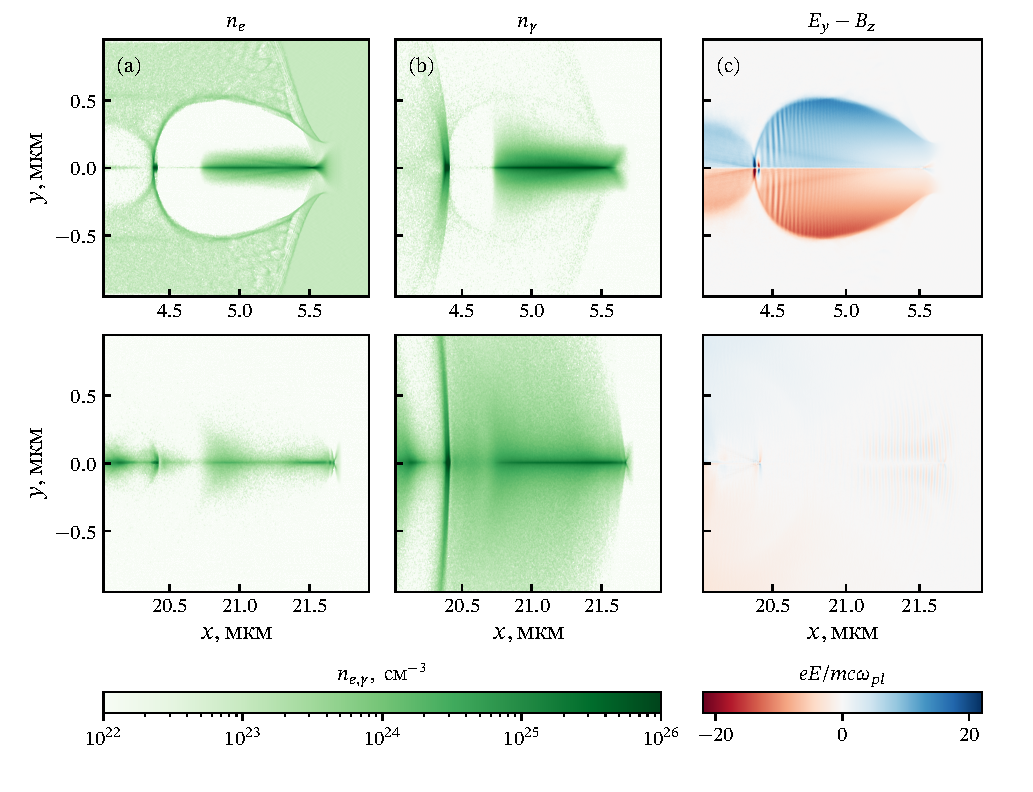
\includegraphics{film-fields.pdf}}
    \caption[Распределение плотности электронов, плотности гамма-фотонов и поперечной силы, действующей на электроны пучка, в моделировании процесса распространения сильноточного пучка в твердотельной мишени]{\label{fig:ch3/bubble} (a) Распределение плотности электронов, (b) плотности гамма-фотонов и (c)~поперечной силы ${E_y - B_z}$, действующей на электроны пучка, в моделировании распространения сильноточного пучка в твердотельной мишени с концентрацией ${n_e=\SI{e23}{\centi\meter^{-3}}}$ и толщиной \SI{10}{\um}. Верхний ряд соответствует проникновению пучка в мишень на глубину \SI{5}{\um}, нижний ряд соответствует моменту выхода пучка из мишени. Координата $x$ отсчитывается от передней границы мишени.}
\end{figure}

Отметим, что недавно была предложена схожая схема для генерации ярких гамма-пучков, основанная на столкновении сильноточного пучка ультрарелятивистских частиц с последовательностью тонких металлических плёнок~\cite{sampath2021extremely}. 
В данной конфигурации эффективное поле, действующее на электроны пучка, связано с <<отражением>> собственного поля пучка от тонкого плазменного слоя, и является по смыслу полем переходного излучения.
Несмотря на различия в физическом механизме генерации гамма-квантов, эффективность генерации и спектр выходного гамма-излучения весьма похожи в конфигурации~\cite{sampath2021extremely} и рассматриваемой нами конфигурации.
Как было описано выше, электроны пучка совершают бетатронные колебания в поле сильно нелинейной кильватерной волны, структура которого описана, например, в публикации~\cite{kostyukov2004phenomenological}.
Для аналитического описания процесса конверсии энергии частиц пучка в энергию гамма-излучения применим разработанную нами в разделе~\ref{sub:ch3/sec3/Long} теорию, описывающую движения частиц одного пучка при столкновении с длинным пучком.
Данную теорию можно без изменений применять к рассматриваемому нами случаю, т.к. конфигурация полей <<баббла>> совпадает с конфигурацией поля встречного пучка, за исключением наличия также тормозящего поля в первом случае.
Таким образом, можно записать
\begin{align}
    \label{eq:ch3/sec3/dydt}
    &\dv{\rho}{t} = -\frac{\rho}{\Gamma}\frac{1}{4\pi}\int_0^{2\pi}P\left(\frac{\rho\Gamma }{2a_\mathrm{S}} | \cos\varphi |\right)\sin^2\varphi \dd\varphi ,\\
    \label{eq:ch3/sec3/dgdt}
    &\dv{\Gamma}{t} = -\frac{1}{2\pi}\int_0^{2\pi}P\left(\frac{\rho \Gamma }{2a_\mathrm{S}} | \cos\varphi |\right) \dd\varphi,
\end{align}
где $\rho$~---~амплитуда бетатронных колебаний, $\Gamma$~---~энергия электрона, $a_\mathrm{S} = mc^2/\hbar\omega_\mathrm{pl}$.
В данных уравнениях используется нормировка на плазменную частоту $\omega_\mathrm{pl}$, соответствующую невозмущённой концентрации электронов мишени $n_e$: время нормировано на $ 1/\omega_\mathrm{pl}$, координаты~---~на $c/\omega_\mathrm{pl}$, импульс~---~на $mc$, напряжённость электромагнитных полей~---~на $mc\omega_\mathrm{pl}/e$, мощность~---~на $mc^2\omega_\mathrm{pl}$.
В классическом ($\chi_0 \ll 1$) и существенно квантовом ($\chi_0 \gg 1$) случаях, когда мощность радиационных потерь $P(\chi)$ является степенной функцией $\chi$, данные уравнения решаются аналитически:
\begin{align}
    \label{eq:ch3/sec3/gamma}
    \frac{ \Gamma(t) }{\gamma_0} \approx 
    \begin{cases}
        {\left(1 + 0.625 P(\chi_0) t / \gamma_0 \right)}^{-4/5},\ \chi\ll 1 \\
        {\left(1 - 0.149 P(\chi_0) t / \gamma_0 \right)}^{24/5},\ \chi\gg 1 \\
    \end{cases}
\end{align}
где $\chi_0 = r_0 \gamma_0 / 2a_\mathrm{S}$, $r_0$~---~начальное отклонение электрона от оси пучка.
Учитывая количество частиц, расположенных внутри мишени, можно окончательно определить зависимость полной энергии пучка от времени:
\begin{equation}
    \label{eq:ch3/coeff}
    \Sigma_e(t) = \Sigma_0 - \int\limits_{-2\sigma_x}^0\int\limits_0^{r_\mathrm{b}}\left( \gamma_0 - \gamma(x + ct) \right) \eta(r, x) \Theta(x + ct) 2 \pi r \dd r \dd x ,
\end{equation}
где $\Sigma_0 = N \gamma_0$, $N$~---~число электронов в пучке, функция $\eta(x, r) = n_\mathrm{b}(x,t)/N$ задаёт распределение заряда в пучке, $\Theta(x)$~---~степ-функция Хевисайда.
Пример сравнения такой оценки с результатами QED-PIC-моделирования представлен на рис.~\ref{fig:ch3/compare},~\ref{fig:ch3/map}.
Отметим, что в данной модели не учитывается наличие продольного поля в плазменной полости, которое дополнительно тормозит электроны пучка.
Этим объясняется различие между оценкой энергии пучка~\eqref{eq:ch3/coeff} и её величиной в численном моделировании.

\begin{figure}
    \center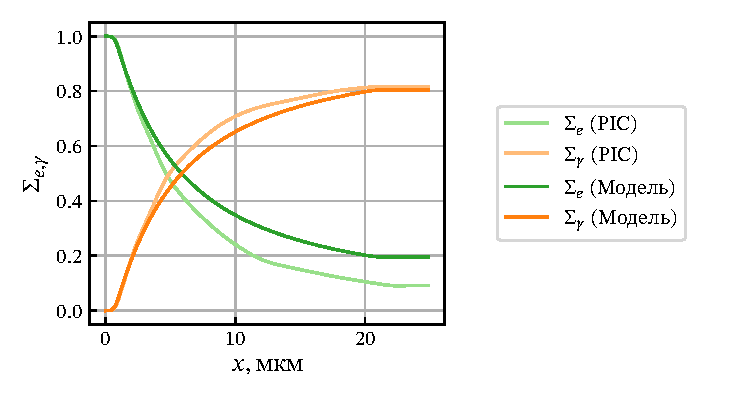
\includegraphics[width=125mm]{film-compare.pdf}
    \caption[Зависимость полной энергии электронов и фотонов от времени при распространении сильноточного пучка в твердотельной мишени]{\label{fig:ch3/compare}
    Зависимость полной энергии электронов $\Sigma_e$ и фотонов $\Sigma_\gamma$ от времени, нормированная на полную начальную энергию электронов.
Сплошные линии соответствуют результатам QED-PIC-моделирования, кружки и квадраты соответствуют оценке, рассчитанной с помощью выражения~\eqref{eq:ch3/coeff} и численного решения уравнений~\eqref{eq:ch3/sec3/dydt}, \eqref{eq:ch3/sec3/dgdt}.}
\end{figure}

\begin{figure}
    \centerfloat{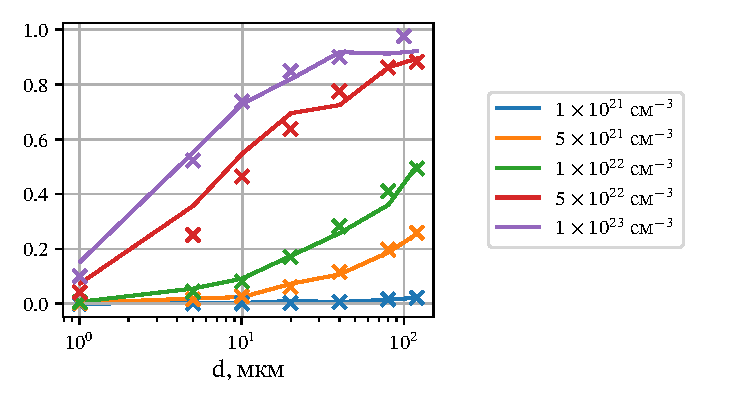
\includegraphics{film-conversion-new.pdf}}
    \caption[Коэффициент конверсии энергии пучка электронов в энергию гамма излучения в зависимости от концентрации и толщины мишени]{\label{fig:ch3/map}
    Коэффициент конверсии энергии пучка электронов в энергию гамма излучения в зависимости от концентрации и толщины мишени: сплошные линии~---~результаты QED-PIC-моделирования, маркеры~---~аналитическая оценка~\eqref{eq:ch3/coeff}.}
\end{figure}

Отметим, что при использованных параметрах пучка даже при столкновении с плотной мишенью, эффективность генерации электрон-позитронных пар из гамма-квантов достаточно мала, для того чтобы существенно повлиять на процесс столкновения.
В связи с этим, в данной работе образование электрон-позитронных пар не рассматривается детально.

Помимо влияния параметров мишени также было исследовано влияние геометрических размеров пучка на эффективность конверсии энергии электронов в энергию гамма-излучения.
В качестве опорных параметров пучка были выбраны параметры, реализованные на установке FACET-II к данному моменту, а именно: заряд пучка от 0.5 до $\SI{3}{\nano\coulomb}$, энергия частиц~---~$\SI{10}{\giga\electronvolt}$, длина пучка $l_\mathrm{b}$ от 1 до $\SI{100}{\um}$, радиус пучка $r_\mathrm{b}$ от 2.5 до $\SI{100}{\um}$.
Как продемонстрировано выше, эффективность конверсии энергии пучка в энергию гамма-излучения, растёт с ростом концентрации и протяжённости мишени.
В связи с этим, в качестве концентрации мишени выбиралась величина равная 0.6 от максимальной концентрации электронов, достигаемой в центре пучка.
Такой выбор обосновывается тем, что при данном соотношении концентраций электронный пучок создаёт в мишени полость, свободную от электронов~---<<\textit{баббл}>>~---~в которой создаётся поперечное поле разделения зарядов.
При этом максимальная толщина мишени ограничивалась характерной длиной свободного пробега по отношению к столкновительным процессам и рассчитывалась из соотношения
\begin{equation}
    % \label{eq:ch3/sec3/freepath}
    l = 10^{-3} \lambda_\sigma = 10^{-3} \left( \sigma_\mathrm{max} n \right)^{-1},
\end{equation}
где $\lambda_\sigma = ( \sigma_\mathrm{max} n )^{-1}$~---~длина свободного пробега по отношению к процессу с сечением $\sigma_\mathrm{max}$, $n$~---~ концентрация рассеивателей (ядер, электронов), которая считалась равной концентрации электронов мишени $n_e$.
При выполнении соотношения~\eqref{eq:ch3/sec3/freepath} столкновительные процессы можно считать несущественными в рассматриваемой задаче. 
Как продемонстрировано выше, потери энергии пучка электронов из-за излучения жёстких фотонов, зависят от двух безразмерных параметров: начального значения КЭД параметра $\chi_0$ и времени взаимодействия пучка с мишенью в плазменных периодах $T = \omega_\mathrm{pl} l / c$.
При этом величина $\chi_0$ вычисляется следующим образом:
\begin{equation}
    \label{eq:ch3/sec3/chi}
    \chi_0 = \gamma_0 n_e r_0 r_e \lambda_C, 
\end{equation}
где $\gamma_0$~---~начальный Лоренц-фактор электронов, $r_0$~---~диаметр пучка, {$r_e$~---~классический радиус электрона}, $\lambda_C$~---~комптоновская длина волны.
В связи с тем, что при параметрах пучка, достижимых на нынешнем этапе развития установки FACET-II, величина параметра $\chi_0$ не превышает значения около 0.2, оценки радиационных потерь можно проводить с помощью формул, соответствующих классическому пределу излучения ($\chi_0 \ll 1$).
В таком случае согласно~\eqref{eq:ch3/sec3/gamma}, эффективность преобразования энергии пучка электронов в гамма излучение можно оценить следующим образом
\begin{equation}
    \label{eq:ch3/sec3/coeff}
    \kappa = \frac{\Sigma_\gamma}{\Sigma_{e,0}} \approx 1 - {\left( 1 + 0.625 P(\chi_0) \right)}^{-4/5},
\end{equation}
где $\Sigma_\gamma$~---~полная энергия гамма-излучения, $\Sigma_{e,0}$~---~начальная энергия электронного пучка, $P(\chi_0) = 2/3 \alpha a_\mathrm{S} \chi_0^2$~---~полная мощность излучения, нормированная на $mc^2\omega_\mathrm{pl}$, $\alpha=e^2/\hbar c$, $a_\mathrm{S} = mc^2/\hbar\omega_\mathrm{pl}$.
Подставляя в~\eqref{eq:ch3/sec3/coeff} значения $T$ и $\chi_0$, выраженные через максимальную концентрацию пучка, можно показать, что величина $\kappa$ пропорциональна максимальной плотности пучка $n_\mathrm{b}$, так же как и величина $\chi_0$, согласно~\eqref{eq:ch3/sec3/chi}.
Таким образом, из оценки~\eqref{eq:ch3/sec3/coeff} следует, что для достижения максимальной конверсии энергии пучка в энергию гамма-излучения, а также генерации излучения с наиболее высокой энергией отсечки (т.к.~максимальная энергия излучаемых фотонов тем больше, чем больше величина $\chi$), необходимо использовать наиболее плотный пучок, что при фиксированном заряде, соответствует минимальным геометрическим размерам пучка. 
Так как наша оценка достаточно простая и получена с учётом ряда предположений, то для более точного определения оптимальных геометрических размеров пучка нами была проведена серия полноразмерных трёхмерных численных моделирований методом частиц-в-ячейках с учётом квантово-электродинамических эффектов, реализованным в коде QUILL~\cite{QUILL}, взаимодействия пучка электронов с однородной мишенью.
В моделировании использовался профиль концентрации пучка, квадратично спадающий по продольной и радиальной координате от геометрического центра пучка.
Заряд и энергия составляли $\SI{3}{\nano\coulomb}$ и $\SI{10}{\giga\electronvolt}$ соответственно.
Результаты проведённого численного моделирования в диапазоне длин пучка от 1 до $\SI{30}{\um}$ и радиусов пучка от 2.5 до $\SI{7.5}{\um}$ представлены на Рис.~\ref{fig:ch3/sec3/Efficiency}.
Согласно результатам моделирования максимальная конверсия энергии пучка в энергию гамма-излучения достигается при минимальном радиусе пучка ($\SI{2.5}{\um}$), но при длине пучка больше минимальной ($\SI{6}{\um}$), и составляет около 12\%.
При этом максимальная энергия фотонов составляет $\SI{4.7}{\giga\electronvolt}$.
  
\begin{figure}[ht]
    \centerfloat{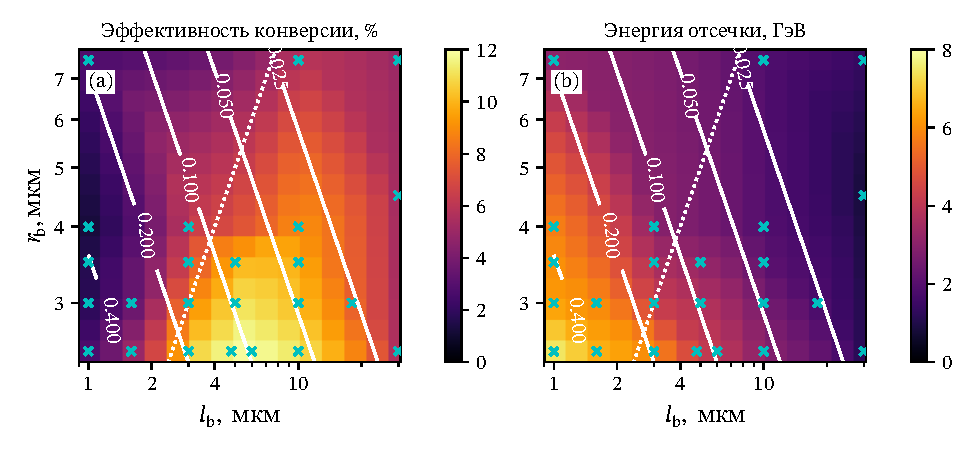
\includegraphics{gamma-map.pdf}}
    \caption[Зависимость эффективности конверсии энергии пучка электронов в энергию гамма-излучения и энергии отсечки в спектре гамма-излучения от длины и радиуса пучка]{Зависимость (a) эффективности конверсии энергии пучка электронов в энергию гамма-излучения и (b) энергии отсечки в спектре гамма-излучения от длины и радиуса пучка.
    Цветовая карта получена с помощью линейной интерполяции между значениями, полученными в результате PIC моделирования (отмечены голубыми маркерами).
    Белая пунктирная линия соответствует равенству $l_\mathrm{b} = r_\mathrm{b}$, белые сплошные линии обозначают уровни постоянного значения $\chi_0$, согласно оценке~\eqref{eq:ch3/sec3/chi}.}
    \label{fig:ch3/sec3/Efficiency}
\end{figure}

Для объяснения причины несоответствия результатов моделирования и нашей оценки нами был подробно рассмотрен процесс формирования баббла (см.~Рис.~\ref{fig:ch3/sec3/Pancake}).
В моделировании с минимально возможными размерами пучка (радиус $r_\mathrm{b} = \SI{2.5}{\um}$, длина $l_\mathrm{b} = \SI{1}{\um}$), его максимальная концентрация равна $\SI{2.8e21}{\centi\meter^{–3}}$, а концентрация мишени соответственно $\SI{1.7e21}{\centi\meter^{–3}}$.
При таких параметрах оценка радиуса баббла согласно модели, разработанной в публикации~\cite{golovanov2021excitation}, даёт величину $\SI{2.8}{\um}$.
Несмотря на то, что поперечное поле разделения зарядов внутри баббла практически не зависит от продольной координаты~\cite{kostyukov2004phenomenological}, оно очевидным образом уменьшается до нуля при переходе через границу баббла (см.~Рис.~\ref{fig:ch3/sec3/Pancake} (b)).
Так как при данных параметрах длина пучка значительно меньше радиуса баббла, а радиус пучка практически совпадает с последним, электроны пучка находятся в области, где напряжённость поперечного поля существенно меньше, чем в основной части баббла (см.~Рис.~\ref{fig:ch3/sec3/Pancake} (b)).
Это приводит к тому, что реальное значение параметра $\chi$ электронов оказывается заметно меньше, чем согласно оценке~\eqref{eq:ch3/sec3/chi}.
В связи с этим излучение электронами фотонов становится неэффективным.
Результаты моделирования показывают, что в целом при взаимодействии пучка электронов с радиусом, превосходящим длительность, эффективность генерации гамма-излучения существенно снижается из-за описанного выше эффекта (см.~пунктирную линию на Рис.~\ref{fig:ch3/sec3/Efficiency} (а)).
При использовании пучка с большей длиной, его существенная часть оказывается в области сильного поперечного поля и теория, разработанная в прошлом году, хорошо описывает конверсию энергии в гамма-излучение. 

\begin{figure}[ht]
    \centerfloat{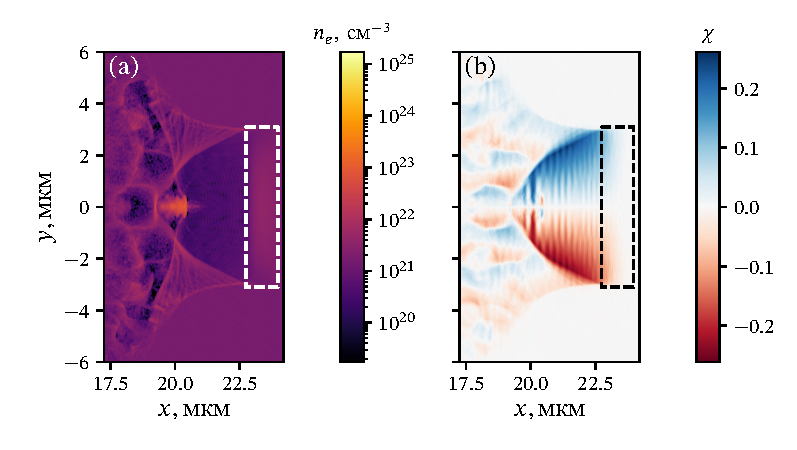
\includegraphics{film-bubble.pdf}}
    \caption[Особенности генерации баббла электронным пучком с диаметром, существенно превосходящим длину]{Особенности генерации баббла электронным пучком с диаметром, существенно превосходящим длину ($l_\mathrm{b} = \SI{1}{\um}$, $r_\mathrm{b} = \SI{2.5}{\um}$). (а) Распределение концентрации электронов и (b) величины $\gamma_0 \left( E_y - B_z \right) / a_\mathrm{S}$, равной значению параметра $\chi$ электронов.
    Координата $x$ отсчитывается от начала мишени.
    Штриховые линии обозначают расположение пучка электронов.}
    \label{fig:ch3/sec3/Pancake}
\end{figure}

Стоит отметить, что несмотря на достижение максимальной эффективности конверсии при длине пучка $\SI{6}{\um}$, с точки зрения приложений получаемого излучения важными также являются его спектральные характеристики.
Результаты моделирования показывают (см.~\ref{fig:ch3/sec3/Efficiency} (b)), что при использовании пучка с минимальными геометрическими размерами, за счёт увеличения значения параметра $\chi_0$, максимальная энергия гамма-фотонов оказывается выше, чем в случае использования пучка с оптимальными параметрами, и достигает $\SI{7.5}{\giga\electronvolt}$.
Однако эффективность генерации при этом оказывается существенно меньше~---~3\%.

\section{Особенности численного моделирования ультрарелятивистских пучков}
\label{sec:ch3/sec4}

Как указывалось выше, развитие технологий ускорителей даст возможность в обозримом будущем проводить беспрецедентные эксперименты по взаимодействию сильноточных пучков заряженных частиц с веществом для генерации гамма-излучения, исследованию процессов сильнополевой КЭД, физики элементарных частиц и даже астрофизических процессов.
В связи с технической сложностью таких экспериментов, крайне важной частью их планирования является поиск оптимальных конфигураций взаимодействия и получение различных качественных и количественных оценок с помощью численного моделирования.
Самым современным методом самосогласованного моделирования динамики плазмы и электромагнитных полей является метод частиц-в-ячейках (PIC).
Несмотря на преимущества данного метода, он не избавлен и от недостатков, одним из которых является дисперсия волн в вакууме, возникающая при использовании стандартной схемы решения уравнений Максвелла~---~схемы \textit{конечных разностей во временной области} (\textit{Finite-Difference Time-Domain}~---~FDTD).
Дисперсия ЭМ волн в вакууме в частности приводит к существованию волн, фазовая скорость которых меньше скорости света.
Таким образом, ультрарелятивистские заряженные частицы могут удовлетворять условию черенковского синхронизма и резонансно возбуждать такие волны в вакууме~---~эффект, известный как {численная черенковская неустойчивость} (\textit{numerical Cherenkov instability}~---~NCI)~\cite{Birdsall1989, Meyers2014, Blinne2017}, который ставит под сомнение достоверность результатов, полученных с помощью численного моделирования.

\begin{figure}[ht]
    \centerfloat{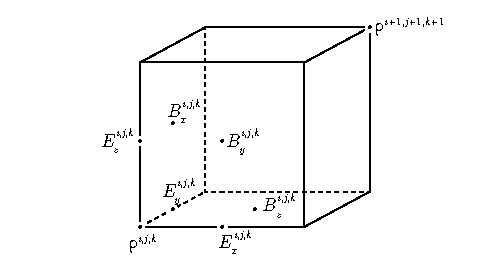
\includegraphics[width=145mm]{beam-QUILL.pdf}}
    \caption{Расположение узлов сеток электрического и магнитного поля и индексы, используемые в комплексе QUILL.}
    \label{fig:ch3/sec4/Quill_indecies}
\end{figure}
Приведём упрощённый анализ, который указывает на причину возникновения численной черенковской неустойчивости (более строгие рассуждения с учётом интерполяции полей на частицы могут быть найдены, например, в работах~\cite{xu2013numerical, godfrey2013numerical}).
Будем использовать расположение и индексирование полей на сетке, использующееся в коде QUILL (см.~Рис.~\ref{fig:ch3/sec4/Quill_indecies}).
Наиболее распространённая схема численного решения уравнений Максвелла~---~схема FDTD (\textit{Finite-Difference Time-Domain}), в которой сетки магнитного и электрического полей смещены на полшага в каждом направлении пространства и во времени, а производные заменяются на конечные разности.
Таким образом уравнения Максвелла переписываются в следующем виде
\begin{align}
    \label{FDTDbx}
    \delta_t B_x &= \delta_z E_y - \delta_y E_z, \\
    \label{FDTDby}
    \delta_t B_y &= \delta_x E_z - \delta_z E_x, \\
    \label{FDTDbz}
    \delta_t B_z &= \delta_y E_x - \delta_x E_y, \\
    \label{FDTDex}
    \delta_t E_x &= \delta_y B_z - \delta_z B_y + j_x, \\
    \label{FDTDey}
    \delta_t E_y &= \delta_x B_x - \delta_x B_z + j_y, \\
    \label{FDTDez}
    \delta_t E_z &= \delta_z B_y - \delta_y B_x + j_z,
\end{align}
где использован оператор конечной разности $\delta$:
\begin{equation}
    \delta_x F^{i+1/2,j,k}=\frac{F^{i+1,j,k}-F^{i,j,k}}{\Delta x}
\end{equation}
который аппроксимирует производную с точностью до $\mathcal{O}({\Delta x}^3)$.
Аналогично определены операторы $\delta_y,\ \delta_z,\ \delta_t$.
Из-за смещения сеток, на которых определены электрическое и магнитное поля, в выражениях \eqref{FDTDbx}--\eqref{FDTDez} значения в левой и правой частях определены в узлах с одинаковым индексом $(i,j,k)$.
Найдём дисперсионное соотношение для волн в вакууме ($\vb{j}=0$).
Для этого будем искать решения уравнений \eqref{FDTDbx}--\eqref{FDTDez} в виде плоских волн, т.е. $\vb{E},\ \vb{B} \propto \exp(-i\omega t + i \vb{kr})$.
Для этого достаточно определить действие оператора $\delta$ на выражение $\exp(-i\omega t + i \vb{kr})$:
\begin{align}
    \delta_\alpha e^{-i\omega t + i \vb{kr}} = \frac{1}{\Delta \alpha} \left( e^{i k_\alpha \Delta \alpha/2} - e^{-i k_\alpha \Delta \alpha/2} \right) e^{-i\omega t + i \vb{kr}} = \frac{2i}{\Delta \alpha} \sin{\frac{k_\alpha \Delta \alpha}{2}} e^{-i\omega t + i \vb{kr}}  \\
    \delta_t e^{-i\omega t + i \vb{kr}} = \frac{1}{\Delta t} \left( e^{-i \omega \Delta t/2} + e^{-i \omega \Delta t/2} \right) e^{-i\omega t + i \vb{kr}} = -\frac{2i}{\Delta t} \sin{\frac{\omega \Delta t}{2}} e^{-i\omega t + i \vb{kr}}
\end{align}
где $\alpha=x,y,z$.
Таким образом, уравнения \eqref{FDTDbx}--\eqref{FDTDez} в вакууме для плоских волн переписываются в виде:
\begin{align}
    \label{FDTDwbx}
    A_t {B_x}_0 = A_y{E_z}_0 - A_z{E_y}_0 \\
    \label{FDTDwby}
    A_t {B_y}_0 = A_z{E_x}_0 - A_x{E_z}_0 \\
    \label{FDTDwbz}
    A_t {B_z}_0 = A_x{E_y}_0 - A_y{E_x}_0 \\
    \label{FDTDwex}
    A_t {E_x}_0 = A_z{B_y}_0 - A_y{B_z}_0 \\
    \label{FDTDwey}
    A_t {E_y}_0 = A_x{B_z}_0 - A_z{B_x}_0 \\
    \label{FDTDwez}
    A_t {E_z}_0 = A_y{B_x}_0 - A_x{B_y}_0
\end{align}
где
\begin{align}
    A_\alpha &=\frac{1}{\Delta\alpha}\sin{\frac{k_\alpha\Delta \alpha}{2}},\ \alpha=x,y,z \\
    A_t &=\frac{1}{\Delta t}\sin{\frac{\omega\Delta t}{2}}
\end{align}
Приравнивая детерминант системы \eqref{FDTDwbx}--\eqref{FDTDwez} к нулю и производя несложные алгебраические преобразования получаем следующее дисперсионное соотношение:
\begin{gather}
    \label{FDTDdisp}
    {A_t}^2={A_x}^2+{A_y}^2+{A_z}^2 \\
    \label{FDTDomega}
    \omega = \pm \frac{2}{\Delta t} \arcsin{\left(\Delta t \sqrt{{A_x}^2+{A_y}^2+{A_z}^2} \right)}
\end{gather}
Данная численная схема устойчива (отсутствует мнимая часть $\omega$) при выполнении условия:
\begin{equation}
    \label{CournatFDTD}
    \frac{1}{{\Delta t}^2} > \frac{1}{{\Delta x}^2} + \frac{1}{{\Delta y}^2} + \frac{1}{{\Delta z}^2}
\end{equation}

\begin{figure}
    \centerfloat{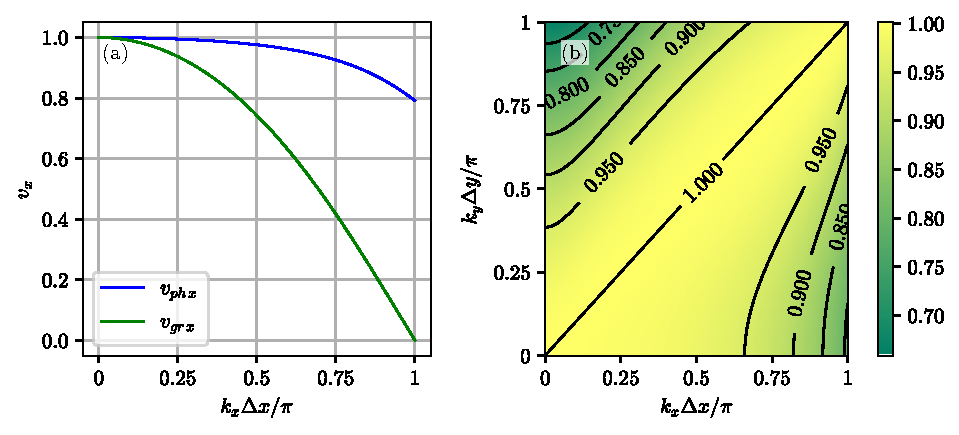
\includegraphics[width=165mm]{beam-FDTD2.pdf}}
    \caption{(a) Зависимость фазовой и групповой скорости волн с $k_z=k_y=0$ от волнового числа $k_x$. (b) Величина фазовой скорости волн c $k_z=0$ в схеме FDTD.}
    \label{fig:ch3/sec4/vphFDTD}
\end{figure}

\begin{figure}
    \centerfloat{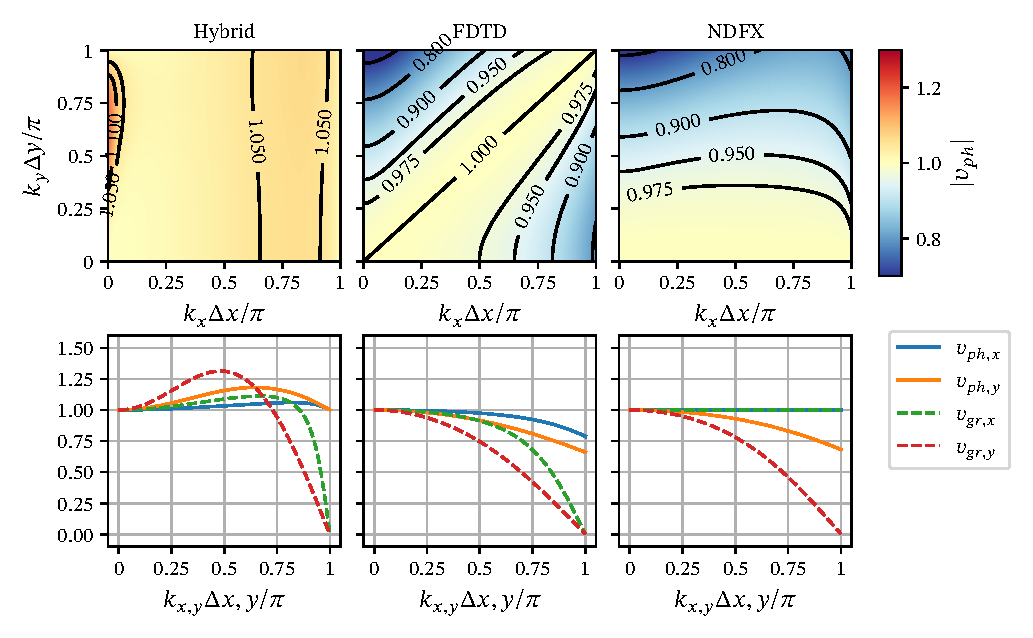
\includegraphics{nci-phase.pdf}}
    \caption{\fixme{(a) Зависимость фазовой и групповой скорости волн с $k_z=k_y=0$ от волнового числа $k_x$. (b) Величина фазовой скорости волн c $k_z=0$ в схеме FDTD.}}
\end{figure}

Модуль фазовой скорости $v_\mathrm{ph} = \omega / |\vb{k}|$ волн с $k_z=0$ представлен на Рис.\ref{fig:ch3/sec4/vphFDTD}.
Видно, что в такой схеме все волны распространяются с фазовой скоростью меньшей скорости света.
Это означает, что частицы, распространяющиеся с околосветовыми скоростями могут двигаться синхронно с такими волнами и возбуждать их.
Генерация таких волн называется численной черенковской неустойчивостью. 

Возбуждение таких волн легко наблюдать в численном моделировании пучка электронов в вакууме.
На Рис.\ref{fig:ch3/sec4/FDTD_NCI} представлены результаты такого моделирования со следующими параметрами: $\Delta t = 0.025$, $\Delta x = 0.05$, $\Delta y = \Delta z = 0.25$, энергия электронов пучка $E_\mathrm{b} = 10$ ГэВ.
Видно наличие нефизичных волн, возбуждаемых таким пучком.
На Фурье-спектре компонент электрического поля (см.~Рис.\ref{fig:ch3/sec4/FDTD_NCI}\;(d)) видно, что для наиболее выраженных гармоник, вычисленная по \eqref{FDTDomega} $x$-компонента фазовой скорости совпадает со скоростью пучка.

\begin{figure}[ht]
	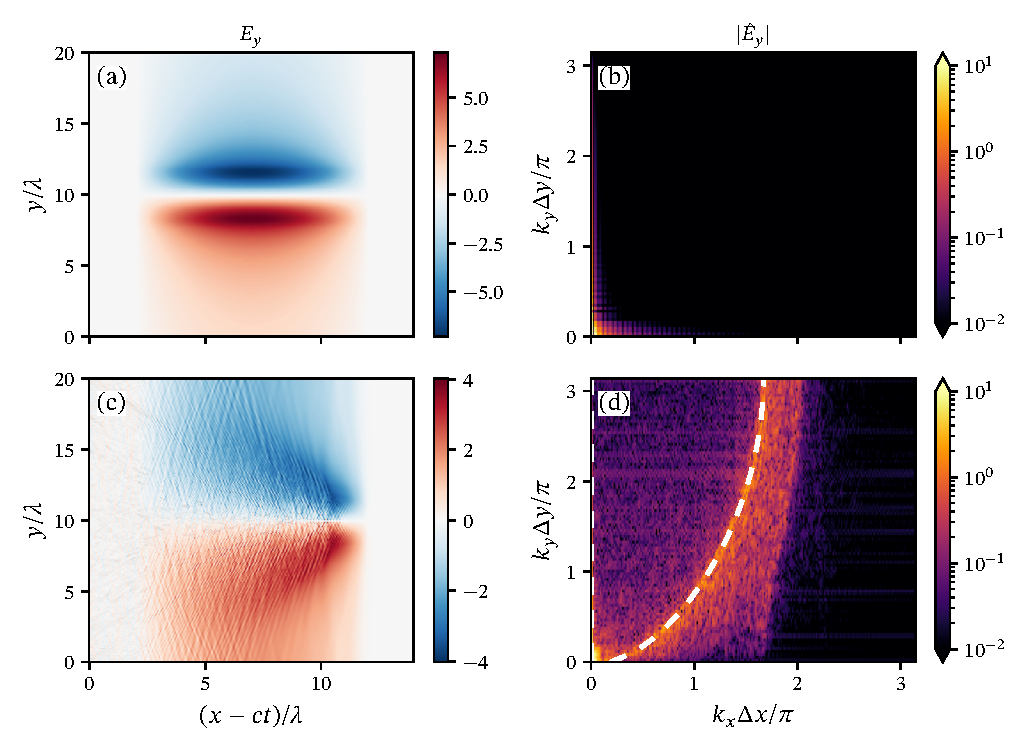
\includegraphics[width=165mm]{beam-NCI_fdtd.pdf} 
	\caption[Результаты численного моделирования ультрарелятивистского ($\gamma~\sim~10^3$) пучка электронов с помощью схемы FDTD]{\label{fig:ch3/sec4/FDTD_NCI} Результаты численного моделирования ультрарелятивистского ($\gamma~\sim~10^3$) пучка электронов с помощью схемы FDTD. (a) Распределение плотности электромагнитного поля (верхняя часть) и плотности электронов (нижняя часть), (b) Фурье-спектр $y$-компоненты электрического поля в начальный момент времени. (c), (d)~---~то же для момента времени $t=400\lambda/c$, где $\lambda=50$ нм~---~условная нормировочная длина.
    Присутствие на спектре гармоник, движущихся со скоростью пучка, свидетельствует о численной черенковской неустойчивости, что также видно по <<разваливанию>> электронного пучка и наличию высокочастотных шумов на распределении плотности электромагнитной энергии.}
\end{figure}

Так как схемы численного решения уравнений Максвелла, основанные на разностных схемах, всегда оперируют с конечной областью в пространстве, то зависимость $\omega(\vb{k})$ для волн в таких схемах всегда периодическая, т.е.~$\omega(\vb{k}+\vb{x}_\alpha N_\alpha 2 \pi / \Delta \alpha)=\omega(\vb{k})$, где $N_\alpha$~---~целое число, $\vb{x}_\alpha$~---~орт в направлении $k_\alpha$, $\alpha=x,y,z$ (так называемый \textit{эффект наложения частот} или \textit{алиасинг}~\cite{Birdsall1989}).
Это означает, что даже если в первой зоне Бриллюэна ($|k_\alpha \Delta \alpha|\leq\pi$) фазовая скорость волн равна или незначительно больше скорости света, то всегда найдётся такая зона Бриллюэна, в которой фазовая скорость будет заведомо меньше скорости света.
Однако, численная черенковская неустойчивость связанна с резонансом частиц и волн в первой зоне Бриллюэна и является линейным эффектом, тогда как эффекты, связанные с резонансом в более дальних зонах,~---~нелинейные и зависят не только от используемой схемы решения уравнений Максвелла, но и от формы частиц, метода интерполяции полей на частицы, метода расчёта тока в узлах решётки и т.д.
Поэтому подавление таких эффектов требует более строгого анализа и до сих пор является не полностью разрешённой проблемой.

В следующем разделе предлагается схема численного решения уравнений Максвелла, в которой фазовая скорость волн в первой зоне Бриллюэна строго больше (но незначительно) скорости света.
Наиболее заметное отклонение фазовой скорости от скорости света в такой схеме у достаточно высокочастотных волн (плохо разрешаемые на сетке) чаще всего не представляющих большой интерес.
Отличие групповой скорости лазерных импульсов с длиной волны, которая хорошо разрешена на сетке ($\lambda_L \gtrsim 10 \Delta x$), сказывается на числе периодов большем, чем характерные времена моделируемых процессов.
Аналогичные рассуждения справедливы и для стандартной схемы FDTD (с тем отличием, что скорость волн в этой схеме меньше скорости света), поэтому можно считать, что предлагаемая нами схема как минимум не хуже схемы FDTD в смысле физической строгости получаемых результатов.


\subsection{Описание схемы численного решения уравнений Максвелла, с подавленной численной черенковской неустойчивостью}
\label{sub:ch3/sec4/Hybrid}

Известно несколько способов подавления NCI, например, использование аппроксимаций более высокого порядка для пространственных производных~\cite{Lu2019, Xu2019, Li2020}, применение фильтров к полям и токам на сетке~\cite{greenwood2004elimination} или использование спектрального подхода к решению уравнений Максвелла в Фурье-пространстве~\cite{Yu2015}, каждое из которых имеет свои преимущества и варианты использования.
Мы предлагаем другую схему ослабления NCI, которая может быть легко реализована в существующих PIC-кодах и которая больше всего подходит для моделирования взаимодействия ультрарелятивистских пучков с плазмой.
Ключевой особенностью нашей схемы является то, что в отличие от схемы FDTD все ЭМ волны в вакууме распространяются со сверхсветовой скоростью.
Это достигается за счёт следующей модификации схемы FDTD
\begin{align}
    \label{eq:ch3/scheme1}
    \delta_t B_x&=(a_{0,z} \delta_zE_y + a_{1,z} \mu_z\delta_zE_y) - (a_{0,y} \delta_yE_z+a_{1,y} \mu_y\delta_y E_z)  ,\\
    \label{eq:ch3/scheme2}
    \delta_t B_y&=(a_{0,x} \delta_xE_z + a_{1,x} \mu_x\delta_xE_z) - (a_{0,z} \delta_zE_x+a_{1,z} \mu_z\delta_z E_x)  ,\\
    \label{eq:ch3/scheme3}
    \delta_t B_z&=(a_{0,y} \delta_yE_x + a_{1,y} \mu_y\delta_yE_x) - (a_{0,x} \delta_xE_y+a_{1,x} \mu_x\delta_x E_y)   ,\\
    \label{eq:ch3/scheme4}
    \delta_t E_x&=(a_{0,y} \delta_yB_z+a_{1,y} \mu_y\delta_yB_z) - (a_{0,z} \delta_zB_y + a_{1,z} \mu_z\delta_zB_y)-j_x ,\\
    \label{eq:ch3/scheme5}
    \delta_t E_y&=(a_{0,z} \delta_zB_x+a_{1,z} \mu_z\delta_zB_x) - (a_{0,x} \delta_xB_z + a_{1,x} \mu_x\delta_xB_z)-j_y ,\\
    \label{eq:ch3/scheme6}
    \delta_t E_z&=(a_{0,x} \delta_xB_y+a_{1,x} \mu_x\delta_xB_y) - (a_{0,y} \delta_yB_x + a_{1,y} \mu_y\delta_yB_x)-j_z ,
\end{align}
\begin{align}
    \label{eq:ch3/sec4/fp-stencil}
    & a_{0,\alpha}+a_{1,\alpha}=1,\ \alpha=x,y,z, \\
    \delta_\alpha F^{j_\alpha+1/2} &= \frac{F^{j_\alpha+1}-F^{j_\alpha}}{\Delta\alpha} ,\ \mu_\alpha F^{j_\alpha} = \frac{F^{j_\alpha+1}+F^{j-1_\alpha}}{2}
\end{align}
Легко показать, что при выполнении условия~\eqref{eq:ch3/sec4/fp-stencil} оператор $\mu_\alpha\delta_\alpha$ аппроксимирует производную $\partial/\partial_\alpha$ с квадратичной точностью.
Решения в вакууме в виде плоских волн уравнений~\eqref{eq:ch3/scheme1}--\eqref{eq:ch3/scheme6} записываются в таком же виде, что и уравнения \eqref{FDTDwbx}--\eqref{FDTDwez}, однако коэффициенты $A_\alpha$ имеют другой вид:
\begin{equation}
    A_\alpha = \frac{1}{\Delta\alpha}\sin{\frac{k_\alpha\Delta \alpha}{2}} \left( a_{0,\alpha}+a_{1,\alpha}\cos{(k_\alpha\Delta\alpha)} \right)
\end{equation}
Дисперсия волн в такой схеме уже зависит от параметров $a_{1,\alpha}$.
Рассмотрим выражение фазовой скорости волн, распространяющихся строго вдоль координатной оси $\alpha$:
\begin{equation}
    v_{\mathrm{ph},\alpha} = 2\frac{\Delta \alpha}{\Delta t}\frac{1}{k_\alpha \Delta \alpha} \arcsin{\left[\frac{\Delta t}{\Delta\alpha}\sin{\frac{k_\alpha\Delta \alpha}{2}} \left( a_{0,\alpha}+a_{1,\alpha}\cos{(k_\alpha\Delta\alpha)}\right) \right]}    
\end{equation}
Из анализа этой функции легко установить, что увеличение коэффициента $a_{1,\alpha}$ приводит к увеличению модуля $v_{\mathrm{ph},\alpha}$ для всех значений $k_\alpha \Delta\alpha$ в первой зоне Бриллюэна ($|k_\alpha \Delta\alpha| \leq \pi$).
Поэтому мы можем найти коэффициенты $a_{1,\alpha}$, например, исходя из требования, чтобы фазовая скорость во всей первой зоне Бриллюэна была больше скорости света и равнялась ей на границах, т.е.
\begin{equation}
    1 = \frac{\Delta \alpha}{\Delta t}\frac{2}{\pi} \arcsin{\left[\frac{\Delta t}{\Delta\alpha}\left( 1 - 2 a_{1,\alpha}\right) \right]}
\end{equation}
Решение этого уравнения записывается в следующем виде
\begin{equation}
    a_{1,\alpha} = \frac{1}{2} \left( 1 - \frac{\Delta \alpha}{\Delta t} \sin{ \left[ \frac{\pi}{2} \frac{\Delta t}{\Delta \alpha} \right]} \right)
\end{equation}
Вычислим максимально возможное значение коэффициентов $A_\alpha$ в таком случае
\begin{equation}
    {A_\alpha}_\mathrm{max} = \frac{1}{\Delta t} \sin{ \left( \frac{\pi}{2} \frac{\Delta t}{\Delta \alpha} \right) }.
\end{equation}
Тогда схема заведомо устойчива при выполнении условия
\begin{equation}
    \text{sin}^2 \left( \frac{\pi}{2} \frac{\Delta t}{\Delta x} \right) + \text{sin}^2 \left( \frac{\pi}{2} \frac{\Delta t}{\Delta y} \right) + \text{sin}^2 \left( \frac{\pi}{2} \frac{\Delta t}{\Delta z} \right) < 1
\end{equation}

Фазовая скорость волн с $k_z=0$ в такой схеме представлена на Рис.\ref{fig:ch3/sec4/vphFDTD}.
Видно, что эти волны распространяются со скоростью большей скорости света, поэтому можно ожидать уменьшения численной черенковской неустойчивости.
Для подтверждения этого мы сравнили результаты идентичных численных расчетов распространения ультрарелятивистского электронного пучка в вакууме с использованием разных схем.
Результаты сравнения показаны на Рис.~\ref{fig:ch3/PIC}.
Ожидаемо, наиболее быстро NCI растет в схеме FDTD; в схеме NDFX, несмотря на точную вакуумную дисперсию волн, распространяющихся вдоль оси распространения пучка, также присутствует неустойчивость.
Это происходит, во-первых, за счет возбуждения распространяющихся под малым углом к оси волн, имеющих фазовую скорость меньше скорости света, и, во-вторых, как было указано выше, за счет пересечения дисперсии пучка и электромагнитных волн вне фундаментальной зоны Бриллюэна (алиасинг).
Очевидно, что предлагаемая нами схема избавляется от первого фактора, так как фазовая скорость всех волн превосходит световую.
Что касается алиасинга, то в целом скорость роста NCI уменьшается с увеличением номера зоны Бриллюэна, поэтому его влияние отсутствует в моделировании в течение достаточно длительного времени ($> 0,12\ пс$).
Моделирование проводилось с использованием кода QUILL~\cite{QUILL}, размеры ячейки составляли $\SI{0.003}{\um}$, $\SI{0.01}{\um}$, $\SI{0.01}{\um}$ по координатам $x$, $y$ и $z$ соответственно.
Временной шаг $\Delta t$ был установлен равным $0.6\Delta x/c$ для предложенной схемы и схемы FDTD и $\Delta x/c$ для схемы NDFX.

% We compared the dispersion relations of proposed hybrid scheme with the typical schemes used in PIC codes: FDTD and NDF~\cite{NDFX}. The results of the comparison are shown in the Fig.~\ref{fig:ch3/vph}.
% As described above in the proposed scheme the phase velocity of all waves in the fundamental Brillouin zone is greater than the speed of light, in contrast to the FDTD scheme, where all the waves propagate slower than the speed of light, and the NDFX scheme, where only the waves propagating along one coordinate axis (in this case, the $x$-axis), have a phase velocity equal to the speed of light.
% The difference between the group velocity and the speed of light, which is present in all schemes, is of the same order of magnitude for all three schemes.

% \begin{figure}
%     \includegraphics[width=165mm]{phase.pdf}
%     \caption{\label{fig:ch3/vph} Phase velocity of the waves propagating in the $xy$-plane ($k_z=0$) (top row), phase and group velocity of the waves propagating along the coordinate ($x$ and $y$) axes (bottom row) in the proposed scheme (a), in the NDFX scheme (b) and in the FDTD scheme(d).}
% \end{figure}



% We also compared the results of the identical numerical simulations of the propagation of an ultrarelativistic electron beam in vacuum using different schemes.
% The comparison results are shown in Fig.~\ref{fig:ch3/PIC}.
% The NCI grows most rapidly in the FDTD scheme.
% In the NDFX scheme, despite the exact vacuum dispersion of the waves propagating along the axis of the beam propagation, instability is also present.
% It occurs firstly due to excitation of the waves propagating at a small angle to the axis which have phase velocity smaller than the speed of light and secondly due to the intersection of the dispersion of the beam and electromagnetic waves outside the fundamental Brillouin zone (the so-called frequency aliasing~\cite{Birdsall1989}).
% Our scheme gets rid of the first factor completely as all the waves are superluminal.
% As for the aliasing in general the growth rate of the NCI decreases with increase of the order of the Brillouin zone, in which the beam and the wave dispersions intersect.
% As seen from the results of the PIC simulations the impact of the aliasing is not present in our scheme for long enough time ($> 0.12\ ps$).
% The simulations were performed using the QUILL code~\cite{QUILL}.
% The simulation the cell size is $0.003 \mu\text m \times 0.01\mu\text m\times 0.01\mu\text m$.
% The time step $\Delta t$ was set to $0.6\Delta x/c$ for the proposed scheme and the FDTD scheme and it was set to $\Delta x/c$ for the NDFX scheme.

% \begin{figure}
%     \includegraphics[width=165mm]{PIC.pdf}
%     \caption{\label{fig:ch3/PIC} Results of the 3D PIC simulations of the ultrarelativistic electron beam propagation in the vacuum. Top row: distribution of the $y$ component of the electric field; bottom row: distribution of the electron density at the initial moment (a) and after 120 fs calculated with the proposed scheme (b), the NDFX scheme (c) and FDTD scheme (d).}
% \end{figure}

Поскольку предложенная схема лишь модифицирует шаблон схемы FDTD, ее можно легко реализовать в существующем коде PIC, по сравнению, например, с недавно предложенной схемой RIP~\cite{Pukhov2019}, которая требует довольно значительной реструктуризации кода.
Отклонение дисперсионного закона от вакуумного в предложенной схеме по сравнению со схемами FDTD или NDF одного порядка и также наиболее существенно в области высоких частот, поэтому при хорошем разрешении интересующих полей на сетки это отклонение может быть пренебрежимо малым.
Таким образом, можно утверждать, что данная схема хорошо подходит для моделирования взаимодействия плотных заряженных пучков со стационарными мишенями, лазерными импульсами или другими пучками, экспериментальная реализация которых ожидается на установке FACET-II в будущем, а также для моделирования лазерно-плазменного взаимодействия, в котором образуются сгустки релятивистских заряженных частиц.

\section{Выводы}

Таким образом, в конфигурации лобового столкновения двух пучков была рассмотрена взаимосвязь процесса фокусировки (или дефокусировки) пучков и излучения частиц.
Была разработана аналитическая модель, которая позволяет рассчитать параметр разрушения с учётом реакции излучения, а также получены упрощённые выражения, достаточные для вычисления порядка величины параметра разрушения.
Было показано, что усиление разрушения из-за пучкового излучения может быть заметным для будущих коллайдеров CLIC и ILC.
В таком случае параметр разрушения увеличивается на несколько десятков процентов, что приводит к дополнительному увеличению яркости.
В приложении же к ускорителю FACET-II, перспективы которого для изучения эффектов непертурбативной КЭД за счёт столкновения пучков обсуждаются в работе~\cite{yakimenko2019prospect}, увеличение параметра разрушения приводит к еще более жестким требованиям к параметрам пучка для прецизионных измерений.
Было показано, что область применимости построенной модели распространяется и на случай столкновения пучков одного заряда.

Также разработана аналитическая модель, описывающая взаимодействие длинных противоположно заряженных пучков в режиме слабого пучкового излучения, когда частицы пучка совершают большое число бетатронных колебаний за время взаимодействия.
Рассчитаны зависимости энергии и амплитуды бетатронных колебаний частицы как в классическом режиме, также и в существенно квантовом режимах.
Прогнозы моделей как в режиме слабого, так сильного пучкового излучения хорошо согласуются с результатами численного моделирования.

Помимо столкновения пучков друг с другом, более технически простой альтернативой для наблюдения КЭД эффектов на установке FACET-II является столкновение одного пучка с протяжённой мишенью.
C помощью полноразмерного трёхмерного численного моделирования нами было обнаружено, что при столкновении сильноточного пучка ультрарелятивистских электронов с протяжённой твердотельной мишенью, генерируются два коротких сгустка гамма-фотонов.
Первый из них связан с излучением электронами начального пучка, а второй~---~с излучением электронами, инжектированными в плазменную полость, создаваемую начальным пучком.
При этом эффективность конверсии энергии пучка электронов в энергию гамма-фотонов может достигать 90\%.
Изученная схема получения гамма-излучения является перспективной с точки зрения простоты экспериментальной реализации и крайне высокой эффективности.

Моделирования и аналитические оценки, проведённые для достигнутых на данный момент параметров пучка на установке FACET-II, показывают, что реально достижимая эффективность конверсии оказывается существенно меньше, однако, всё равно достигает более десяти процентов.
Также было продемонстрировано, что использование пучка в виде <<блина>>, т.е. с диаметром пучка, превосходящим его длину, является не эффективным даже достижении большей концентрации пучка, что связанно с тем, что в таком случае лишь малая часть частиц оказывается в области сильного плазменного поля.

Также нами была разработана и реализована в коде QUILL альтернативная схема для численного решения уравнений Максвелла на прямоугольной сетке.
С помощью данной схемы, нами были проведены численные моделирования взаимодействия сильноточных пучков ультрарелятивистских частиц друг с другом и с плазменной мишенью.

Основные полученные в данной главе результаты опубликованы в работах~\cite{samsonov2020superluminal, samsonov2021beamstrahlung, filipovic2021effect, samsonov2022simulation,samsonov2020Math, samsonov2021LPHYS}

\FloatBarrier           % Глава 3
\chapter*{Заключение}                       % Заголовок
\addcontentsline{toc}{chapter}{Заключение}  % Добавляем его в оглавление

%% Согласно ГОСТ Р 7.0.11-2011:
%% 5.3.3 В заключении диссертации излагают итоги выполненного исследования, рекомендации, перспективы дальнейшей разработки темы.
%% 9.2.3 В заключении автореферата диссертации излагают итоги данного исследования, рекомендации и перспективы дальнейшей разработки темы.
%% Поэтому имеет смысл сделать эту часть общей и загрузить из одного файла в автореферат и в диссертацию:

Основные результаты работы заключаются в следующем.
%% Согласно ГОСТ Р 7.0.11-2011:
%% 5.3.3 В заключении диссертации излагают итоги выполненного исследования, рекомендации, перспективы дальнейшей разработки темы.
%% 9.2.3 В заключении автореферата диссертации излагают итоги данного исследования, рекомендации и перспективы дальнейшей разработки темы.
\fixme{Скопированная новизна}
\begin{enumerate}[beginpenalty=10000] % https://tex.stackexchange.com/a/476052/104425
  \item Разработана асимптотическая теория движения заряженных частиц в режиме экстремальных радиационных потерь. Определены общие свойства движения частиц в таком режиме, существенно отличающиеся от таковых в режиме слабой реакции излучения. Продемонстрирован новый метод получения приближённого решения уравнений движения в различных конфигурациях.
  \item Обнаружен и качественно описан эффект развития самоподдерживающегося квантово-электродинамического каскада в поле, приближенном к полю плоской волны. Разработана аналитическая модель, описывающая развитие такого каскада.
  \item Разработана модель для вычисления параметра разрушения при лобовом столкновении сильноточных пучков ультрарелятивистских частиц с учётом реакции излучения. Достоверность модели подтверждена полноразмерным численным трёхмерным моделированием
  \item С помощью полноразмерного трёхмерного численного моделирования продемонстрирована схема эффективной генерации гамма-излучения при взаимодействии сильноточного пучка ультрарелятивистских электронов с протяжённой плазменной мишенью. Разработана аналитическая модель для вычисления эффективности конверсии энергии пучка в энергию гамма-излучения. Найдены параметры пучка для установки FACET-II, оптимальные с точки зрения генерации гамма-излучения.
  \item Разработана и реализована в коде QUILL альтернативная схема для численного решения уравнений Максвелла на регулярной сетке, отличающаяся существенно подавленной численной черенковской неустойчивостью, и подходящей для моделирования пучков ультрарелятивистских частиц.
\end{enumerate}


\vspace{0.25cm}
В заключении, автор хотел бы выразить свою искреннюю благодарность и признательность своему научному руководителю, Игорю Юрьевичу Костюкову, за его ценную поддержку, активное обсуждение результатов и научное руководство на протяжении всего исследования.
Также автор выражает глубокую признательность Евгению Николаевичу Нерушу за его ценные советы, помощь в разработке численных моделей и важные обсуждения результатов. 
Автор благодарит Антона Александровича Голованова и Евгения Николаевича Неруша за разработку PIC-кода Quill, который был использован при получении значительной части результатов, а также за их ценную помощь в модификации данного кода. 
Наконец, автор выражает благодарность всем, кто помогал в создании этой работы и внес свой вклад в ее успешное завершение.      % Заключение
% \include{Dissertation/acronyms}        % Список сокращений и условных обозначений
% \include{Dissertation/dictionary}      % Словарь терминов

\setcounter{totalchapter}{\value{chapter}} % Подсчёт количества глав

%%% Настройки для приложений
\appendix
% Оформление заголовков приложений ближе к ГОСТ:
\setlength{\midchapskip}{20pt}
\renewcommand*{\afterchapternum}{\par\nobreak\vskip \midchapskip}
\renewcommand\thechapter{\Asbuk{chapter}} % Чтобы приложения русскими буквами нумеровались

\chapter{Численное решение релятивистских уравнений движения заряженной частицы}
\label{app:numerical}

Релятивистские уравнения движения электрона во внешнем ЭМ поле с учётом реакции излучения записываются в следующем виде
\begin{gather}
    \label{eq:app/base1}
    \dv{\gamma}{t} = -\vb{vE} - F_\mathrm{rr} v^2 , \\
    \label{eq:app/base2}
    \dv{\vb{p}}{t} = - \vb{E - v\times B} - F_\mathrm{rr}\vb{v},
\end{gather}
где импульс электрона $\vb{p}$ нормирован на $m c$, время $t$~---~на $1/\omega$, электрическое и магнитное поля~---~на $m c \omega / e$, $F_\mathrm{rr}$~---~полная мощность излучения, нормированная $mc^2\omega$.
Для численного решения уравнений~\eqref{eq:app/base1}--\eqref{eq:app/base2} без учёта реакции излучения ($F_\mathrm{rr}=0$) существует несколько методов, таких как схема Бориса (Boris)~\cite{boris1970relativistic}, схема Вэя (Vay)~\cite{Vay08} и схема Игэры-Карри (Higuera-Cary, HC)~\cite{higuera2017structure}. 
Последняя из этих схем наиболее точно сохраняет Гамильтониан системы (а значит и фазовый объём), поэтому именно она используется в данной работе при решении уравнений движения одной частицы в заданных полях.
Явный вид данной схемы записывается в следующем виде
\begin{gather}
    \vb{r}_{i+1} = \vb{r}_i + \Delta t \frac{\vb{p}_{i+1/2}}{\gamma_{i+1/2}}, \\
    \vb{p}_{i+1/2} = \tilde{\vb{p}} - \frac{\hat{\vb{p}} }{\hat{\gamma}} \times \symbf{\beta},
\end{gather}
где $\tilde{\vb{p}} = \vb{p}_{i-1/2} - \symbf{\epsilon}$, $\tilde{\gamma} = \sqrt{1 + \tilde{\vb{p}}\cdot\tilde{\vb{p}}}$, $\symbf{\epsilon} = \vb{E}\Delta t / 2$, $\symbf{\beta} = \vb{B} \Delta t / 2$, a $\hat{\vb{p}}$ и $\hat{\gamma}$~---~промежуточные значения импульса и энергии электрона соответственно, вычисляемые следующим образом
\begin{gather}
    \hat{\gamma}^2 = \frac{1}{2}\left( \tilde{\gamma}^2 - \beta^2 + \sqrt{\left( \tilde{\gamma}^2 - \beta^2 \right)^2 + 4 \left( \beta^2 + {\left|\symbf{\beta}\cdot\tilde{\vb{p}}\right|}^2 \right)} \right), \\
    \hat{\vb{p}} = \left( \tilde{\vb{p}} - \frac{\symbf{\beta} \times \tilde{\vb{p}}}{\hat{\gamma}} + \symbf{\beta} \frac{\symbf{\beta}\cdot\tilde{\vb{p}}}{\hat{\gamma}^2} \right) \left( 1 + \frac{\beta^2}{\hat{\gamma}^2} \right)^{-1}.
\end{gather}
Отметим, что координаты (и ЭМ поля) и импульсы электрона определены в моменты времени, смещённые на половину шага $\Delta t$ относительно друг друга, что объясняет полуцелые индексы у импульсов.

Для учёта реакции излучения используется два различных подхода.
В первом, полуклассическом подходе (обозначается на рисунках аббревиатурой LL), радиационное трение считается непрерывной силой, которая добавляется в численную схему по методу Эйлера следующим образом: сначала делается шаг по схеме Игеры-Кары и вычисляется импульс $\vb{p}_{\mathrm{HC}, i+1/2}$, затем конечный импульс электрона определяется следующим образом
\begin{gather}
    \vb{p}_{i+1/2} = \vb{p}_{\mathrm{HC}, i+1/2} - \Delta t F_\mathrm{rr} (\bar{\chi}) \frac{\bar{\vb{p}}}{\bar{\gamma}} , \\
    \bar{\chi} = \frac{1}{a_\mathrm{S}}\sqrt{\left( \bar{\gamma} \vb{E} + \bar{\vb{p}}\times\vb{B} \right)^2 - \left( \bar{\vb{p}} \cdot E \right)^2}, \\
    \bar{\vb{p}} = \frac{\vb{p}_{i-1/2} + \vb{p}_{\mathrm{HC}, i+1/2}}{2}, \\
    \bar{\gamma} = \sqrt{1 + \bar{\vb{p}}\cdot\bar{\vb{p}}},
\end{gather} 
где $a_\mathrm{S} = mc^2 / \hbar\omega$~---~нормированное критическое поле Заутера-Швингера.
Во втором подходе (обозначается на рисунках аббревиатурой MC) учитывается квантовая (стохастическая) природа излучения с помощью метода Монте-Карло схожим образом с методом, реализованным в комплексе QUILL~\cite{QUILL, elkina2011qed}: на каждом шаге разыгрываются два равномерно распределённых в интервале $[0, 1]$ случайных числа $r_0$ и $r_1$; затем вычисляется вероятность $W$ излучения электроном фотона с энергией $r_0 \bar{\gamma}$ за промежуток времени $\Delta t$; если выполняется неравенство $r_1 < W$, то от конечного импульса электрона $\vb{p}_{\mathrm{HC}, i+1/2}$ отнимается величина $r_0 \bar{\vb{p}}$, в противном случае конечный импульс электрона не изменяется.
Величина $W$ вычисляется следующим образом~\cite{Baier98}
\begin{gather}
    W = \Delta t \frac{ \alpha a_\mathrm{S}}{\sqrt{3}\pi\bar{\gamma}} \left( \frac{r_0^2 - 2 r_0 + 2}{1 - r_0}K_{2/3}( y ) - \int\limits_y^{+\infty} K_{1/3}(x)\dd x \right), \\
    y = \frac{r_0}{1 - r_0}\frac{2}{3 \bar{\chi}},
\end{gather}
где $K_\nu(x)$~---~модифицированная функция Бесселя второго рода.

Другие различные дифференциальные уравнения в данной работе решаются с помощью адаптивного метода Рунге-Кутты 8-го порядка (DOP853~\cite{hairer1993solving}), если не указано другое.        % Приложения

\setcounter{totalappendix}{\value{chapter}} % Подсчёт количества приложений

\clearpage                                  % В том числе гарантирует, что список литературы в оглавлении будет с правильным номером страницы
%\hypersetup{ urlcolor=black }               % Ссылки делаем чёрными
%\providecommand*{\BibDash}{}                % В стилях ugost2008 отключаем использование тире как разделителя
\urlstyle{rm}                               % ссылки URL обычным шрифтом
\ifdefmacro{\microtypesetup}{\microtypesetup{protrusion=false}}{} % не рекомендуется применять пакет микротипографики к автоматически генерируемому списку литературы
% \insertbibliofull                           % Подключаем Bib-базы: все статьи единым списком
% Режим с подсписками
\insertbiblioexternal                      % Подключаем Bib-базы: статьи, не являющиеся статьями автора по теме диссертации
% Для вывода выберите и расскомментируйте одно из двух
\insertbiblioauthor                        % Подключаем Bib-базы: работы автора единым списком 
%\insertbiblioauthorgrouped                 % Подключаем Bib-базы: работы автора сгруппированные (ВАК, WoS, Scopus и т.д.)
\ifdefmacro{\microtypesetup}{\microtypesetup{protrusion=true}}{}
\urlstyle{tt}                               % возвращаем установки шрифта ссылок URL
%\hypersetup{ urlcolor={urlcolor} }          % Восстанавливаем цвет ссылок
      % Список литературы
\clearpage
\ifdefmacro{\microtypesetup}{\microtypesetup{protrusion=false}}{} % не рекомендуется применять пакет микротипографики к автоматически генерируемым спискам
\listoffigures  % Список изображений

%%% Список таблиц %%%
% (ГОСТ Р 7.0.11-2011, 5.3.10)
% \clearpage
% \listoftables   % Список таблиц
% \ifdefmacro{\microtypesetup}{\microtypesetup{protrusion=true}}{}
% \newpage           % Списки таблиц и изображений (иллюстративный материал)

\end{document}